\section{Results}

\begin{figure}[H]
% This file was created by matlab2tikz.
%
%The latest updates can be retrieved from
%  http://www.mathworks.com/matlabcentral/fileexchange/22022-matlab2tikz-matlab2tikz
%where you can also make suggestions and rate matlab2tikz.
%
\definecolor{mycolor1}{rgb}{0.06600,0.44300,0.74500}%
\definecolor{mycolor2}{rgb}{0.12941,0.12941,0.12941}%
\definecolor{mycolor3}{rgb}{0.86600,0.32900,0.00000}%
%
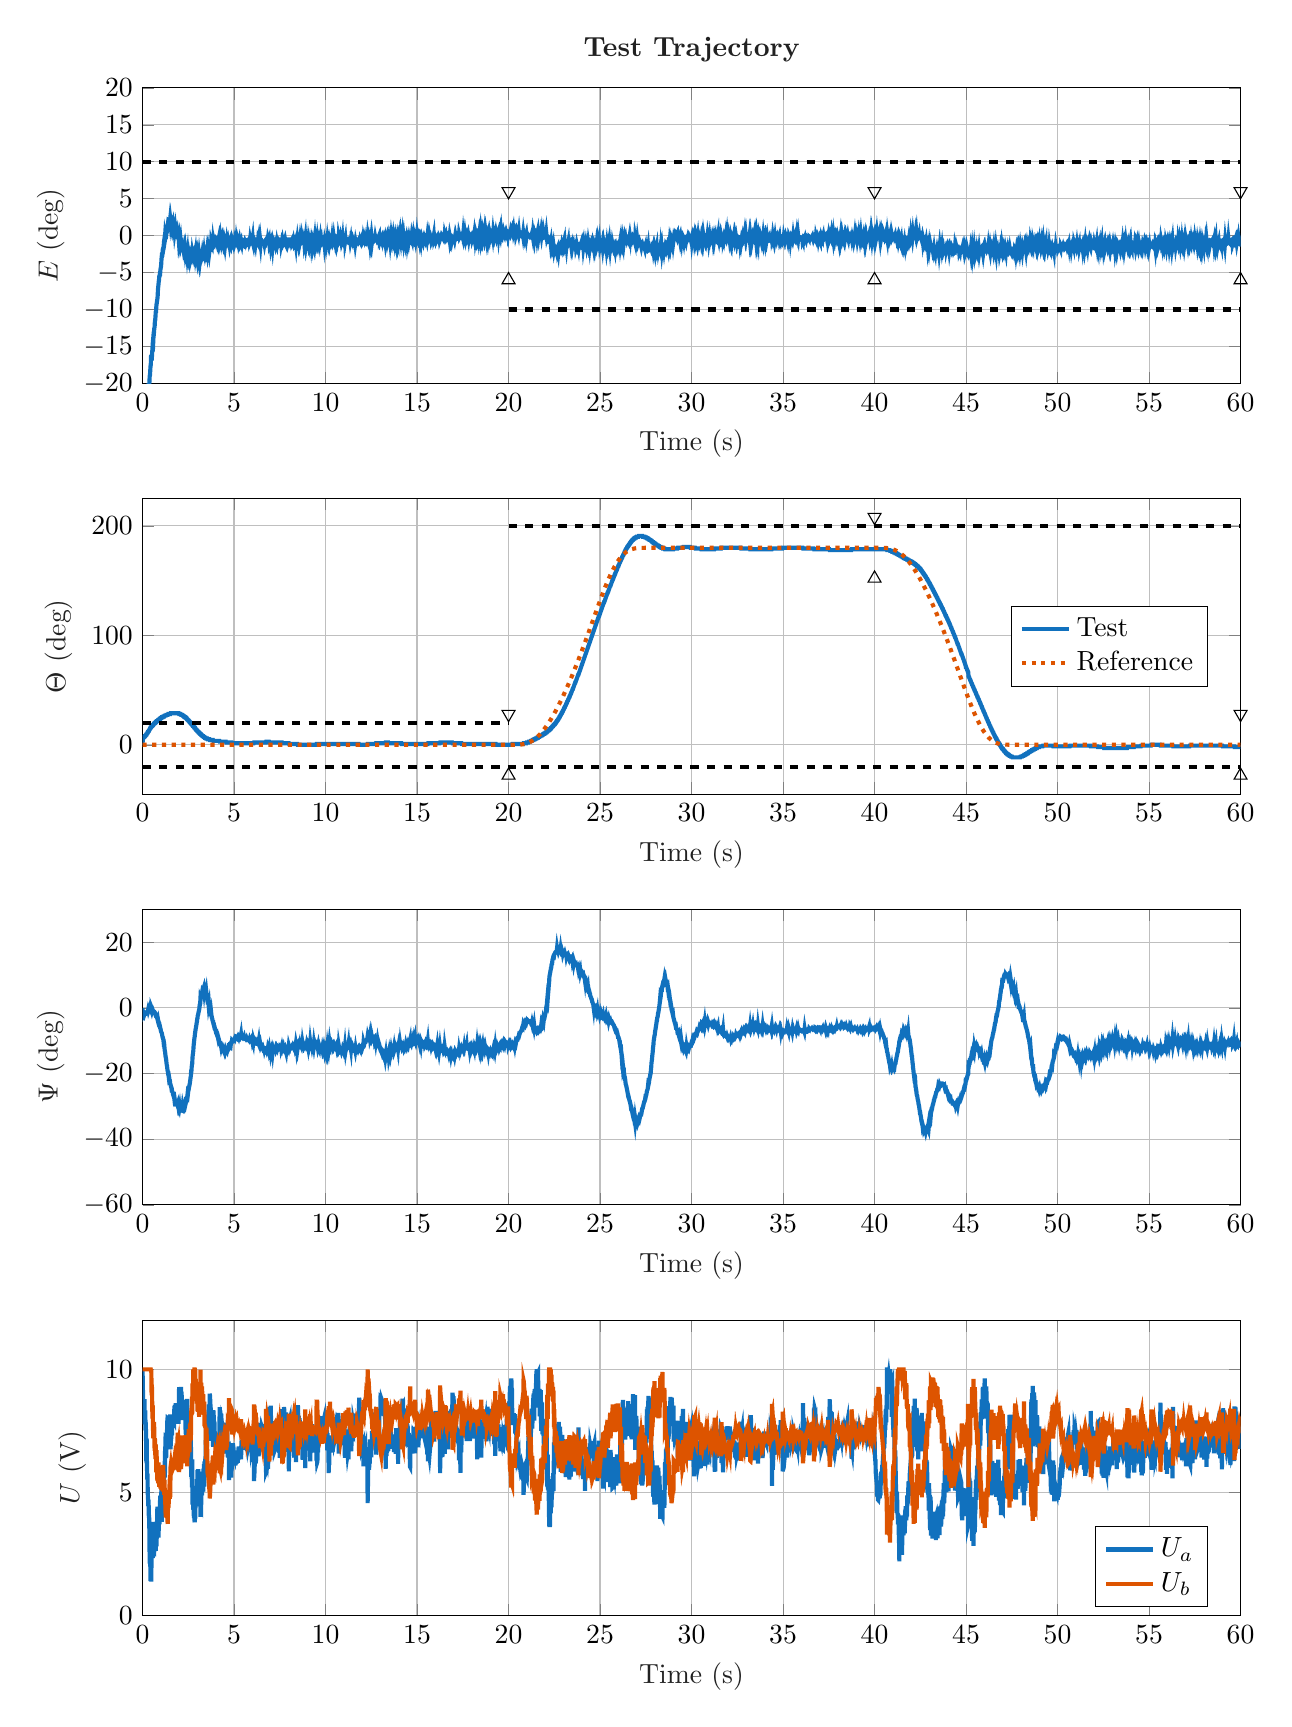
\begin{tikzpicture}

\begin{axis}[%
width=5.49in,
height=1.478in,
at={(0.921in,7.193in)},
scale only axis,
xmin=0,
xmax=60,
xlabel style={font=\color{mycolor2}},
xlabel={Time (s)},
ymin=-20,
ymax=20,
ytick={-20, -15, -10,  -5,   0,   5,  10,  15,  20},
ylabel style={font=\color{mycolor2}},
ylabel={$E$ (deg)},
axis background/.style={fill=white},
title style={font=\bfseries\color{mycolor2}},
title={Test Trajectory},
xmajorgrids,
ymajorgrids
]
\addplot [color=mycolor1, line width=1.5pt, forget plot]
  table[row sep=crcr]{%
0	-26.4082312686148\\
0.015	-26.5122763107205\\
0.03	-25.7100342755372\\
0.045	-25.9537187162584\\
0.06	-25.5238484107164\\
0.075	-25.6717018916035\\
0.09	-25.4718258896636\\
0.105	-25.4033752040677\\
0.12	-25.2609977780284\\
0.135	-24.7955331159766\\
0.15	-24.6312514705466\\
0.165	-24.5107782638979\\
0.18	-24.2972121248389\\
0.195	-24.1548346987995\\
0.21	-23.8536516821778\\
0.225	-23.4292574314835\\
0.24	-23.1034321680473\\
0.255	-23.0404575372991\\
0.27	-22.5284464090421\\
0.285	-22.4380915040556\\
0.3	-21.4359734669324\\
0.315	-21.5454945638858\\
0.33	-21.2415735198402\\
0.345	-20.9020581192848\\
0.36	-20.2257653455978\\
0.375	-19.8807738901948\\
0.39	-19.0210332791109\\
0.405	-18.8759178256477\\
0.42	-18.2981940392187\\
0.435	-17.6629716768893\\
0.45	-17.4795238394924\\
0.465	-16.3268142940583\\
0.48	-16.2966959923962\\
0.495	-16.4281213087402\\
0.51	-16.4500255281309\\
0.525	-15.8120651383776\\
0.54	-15.376718777988\\
0.555	-14.6757837574865\\
0.57	-14.2568655616399\\
0.585	-14.3526965214741\\
0.6	-13.5531925137146\\
0.615	-13.4464094441851\\
0.63	-12.8686856577561\\
0.645	-12.5017899829624\\
0.66	-12.3320322826847\\
0.675	-11.5763367137065\\
0.69	-11.4640775893293\\
0.705	-11.0150410918205\\
0.72	-10.3661285923719\\
0.735	-10.3250581810144\\
0.75	-9.69257384610877\\
0.765	-9.28460775995751\\
0.78	-9.0819937305938\\
0.795	-8.77807268654825\\
0.81	-8.5727206297607\\
0.825	-8.21403903723845\\
0.84	-7.40084489235978\\
0.855	-6.96549853197019\\
0.87	-6.63145918626245\\
0.885	-6.19885085329669\\
0.9	-5.98254668681381\\
0.915	-5.49791583279521\\
0.93	-5.44863133916621\\
0.945	-5.15566240481597\\
0.96	-5.16113845966364\\
0.975	-4.6409132491352\\
0.99	-4.41913302780465\\
1.005	-4.21651899844094\\
1.02	-3.8660514881902\\
1.035	-3.19249674192706\\
1.05	-2.79274473804731\\
1.065	-2.82286303970948\\
1.08	-2.74072221699447\\
1.095	-2.32180402114788\\
1.11	-1.8070548654671\\
1.125	-1.69479574108991\\
1.14	-1.67836757654691\\
1.155	-1.43468313582569\\
1.17	-0.859697376820566\\
1.185	-0.599584771556347\\
1.2	-0.804936828343894\\
1.215	-0.566728442470338\\
1.23	-0.0382891496703934\\
1.245	-0.25733134357711\\
1.26	-0.0245990125512237\\
1.275	0.350510744514023\\
1.29	0.460031841467381\\
1.305	0.394319183295363\\
1.32	0.758476830665278\\
1.335	0.947400722909809\\
1.35	0.909068338976138\\
1.365	1.19382319105487\\
1.38	1.47923500306085\\
1.395	1.38590786056536\\
1.41	1.49673384227875\\
1.425	1.86712593905772\\
1.44	1.40340669978326\\
1.455	1.8525435730428\\
1.47	1.80879647499804\\
1.485	1.72130227890852\\
1.5	2.05961317045466\\
1.515	1.73296817172045\\
1.53	2.05378022404869\\
1.545	1.76213290375029\\
1.56	1.8700424122607\\
1.575	1.80296352859207\\
1.59	1.61047629719513\\
1.605	2.05669669725168\\
1.62	1.52881504751158\\
1.635	1.70963638609658\\
1.65	1.83504473382489\\
1.665	1.46173616384294\\
1.68	1.70088696648763\\
1.695	1.60172687758617\\
1.71	1.55506330633843\\
1.725	1.50256678868472\\
1.74	1.043231682744\\
1.755	1.33341134291165\\
1.77	0.7283585290031\\
1.785	0.977519024571987\\
1.8	0.62978954174508\\
1.815	0.498364225401052\\
1.83	0.616099404625911\\
1.845	0.345034689666353\\
1.86	0.394319183295363\\
1.875	0.271107949222835\\
1.89	0.438127622076711\\
1.905	0.0986122215212972\\
1.92	-0.0875736432994032\\
1.935	-0.147810246623752\\
1.95	-0.235427124186433\\
1.965	0.0657558924352954\\
1.98	-0.490063674602989\\
1.995	-0.25733134357711\\
2.01	-0.599584771556347\\
2.025	-0.30661583720612\\
2.04	-0.917195952721083\\
2.055	-0.722796005628875\\
2.07	-0.974694528621593\\
2.085	-0.711843895933536\\
2.1	-1.09516773527028\\
2.115	-1.04314521421744\\
2.13	-1.40182680673968\\
2.145	-1.49491973915003\\
2.16	-1.55241831505055\\
2.175	-1.58527464413655\\
2.19	-1.22111699676664\\
2.205	-1.64824927488474\\
2.22	-1.60991689095106\\
2.235	-1.85633935909611\\
2.25	-1.66467743942774\\
2.265	-2.03704916906915\\
2.28	-1.97133651089713\\
2.295	-2.08085760785049\\
2.31	-2.15478434829401\\
2.325	-1.90562385272512\\
2.34	-2.28894769206187\\
2.355	-2.07538155300282\\
2.37	-2.27799558236653\\
2.385	-1.47849157460704\\
2.4	-2.34644626796238\\
2.415	-2.56001240702143\\
2.43	-2.22049700646602\\
2.445	-2.63393914746494\\
2.46	-2.34097021311471\\
2.475	-2.78179262835197\\
2.49	-2.65858139427945\\
2.505	-2.5983447909551\\
2.52	-2.84750528652399\\
2.535	-2.60929690065044\\
2.55	-2.84202923167632\\
2.565	-2.71334194275613\\
2.58	-3.00904890453018\\
2.595	-2.7516743266898\\
2.61	-2.88309964303383\\
2.625	-2.72429405245146\\
2.64	-2.80917290259031\\
2.655	-2.22597306131368\\
2.67	-2.75441235411364\\
2.685	-2.60108281837894\\
2.7	-2.67227153139862\\
2.715	-3.12952211117888\\
2.73	-2.54084621505459\\
2.745	-2.76262643638514\\
2.76	-2.64762928458412\\
2.775	-2.97893060286801\\
2.79	-2.91047991727217\\
2.805	-3.05559537073536\\
2.82	-2.89131372530533\\
2.835	-2.70238983306079\\
2.85	-3.01726298680169\\
2.865	-2.4285870906774\\
2.88	-2.71607997017996\\
2.895	-2.4450152552204\\
2.91	-2.89405175272916\\
2.925	-2.70786588790846\\
2.94	-3.0994038095167\\
2.955	-2.66679547655095\\
2.97	-2.89952780757683\\
2.985	-2.64489125716028\\
3	-2.95976441090118\\
3.015	-2.65858139427945\\
3.03	-2.7106039153323\\
3.045	-2.94333624635817\\
3.06	-2.69417575078929\\
3.075	-2.96250243832501\\
3.09	-2.62846309261728\\
3.105	-2.95428835605351\\
3.12	-2.53263213278309\\
3.135	-2.65036731200795\\
3.15	-2.97893060286801\\
3.165	-2.65310533943178\\
3.18	-2.52168002308775\\
3.195	-2.53537016020692\\
3.21	-2.84202923167632\\
3.225	-2.66953350397479\\
3.24	-2.76810249123281\\
3.255	-2.77357854608047\\
3.27	-2.48882369400174\\
3.285	-2.7188179976038\\
3.3	-2.61477295549811\\
3.315	-2.56275043444526\\
3.33	-2.65310533943178\\
3.345	-2.38477865189606\\
3.36	-2.79274473804731\\
3.375	-2.40394484386289\\
3.39	-2.40942089871057\\
3.405	-2.22049700646602\\
3.42	-2.22049700646602\\
3.435	-2.51620396824008\\
3.45	-2.36013640508155\\
3.465	-2.47787158430641\\
3.48	-2.3081138840287\\
3.495	-2.25609136297586\\
3.51	-2.32728007599555\\
3.525	-2.02609705937381\\
3.54	-2.28073360979036\\
3.555	-1.96312242862563\\
3.57	-1.71943798790442\\
3.585	-2.00693086740697\\
3.6	-1.98228862059247\\
3.615	-2.07264352557899\\
3.63	-1.74408023471892\\
3.645	-1.66467743942774\\
3.66	-2.00966889483081\\
3.675	-1.71669996048059\\
3.69	-1.74408023471892\\
3.705	-1.70300982336142\\
3.72	-1.73039009759975\\
3.735	-1.59896478125573\\
3.75	-0.903505815601913\\
3.765	-1.05135929648894\\
3.78	-1.30325781948166\\
3.795	-1.39087469704435\\
3.81	-0.936362144687915\\
3.825	-1.28135360009099\\
3.84	-1.28409162751482\\
3.855	-0.804936828343894\\
3.87	-1.07052548845578\\
3.885	-1.12528603693246\\
3.9	-0.761128389562546\\
3.915	-0.930886089840253\\
3.93	-0.958266364078592\\
3.945	-0.700891786238198\\
3.96	-0.613274908675517\\
3.975	-0.725534033052706\\
3.99	-0.610536881251679\\
4.005	-0.514705921417497\\
4.02	-0.585894634437177\\
4.035	-0.728272060476537\\
4.05	-0.402446797040308\\
4.065	-0.37232849537813\\
4.08	-0.490063674602989\\
4.095	-0.632441100642356\\
4.11	-0.574942524741839\\
4.125	-0.473635510059981\\
4.14	-0.744700225019545\\
4.155	-0.533872113384329\\
4.17	-0.344948221139791\\
4.185	-0.657083347456857\\
4.2	-0.955528336654754\\
4.215	-0.769342471834047\\
4.23	-0.657083347456857\\
4.245	-0.802198800920056\\
4.26	-0.824103020310726\\
4.275	-0.427089043854809\\
4.29	-0.673511511999858\\
4.305	-0.898029760754244\\
4.32	-0.689939676542866\\
4.335	-0.525658031112829\\
4.35	-0.881601596211236\\
4.365	-0.969218473773924\\
4.38	-0.870649486515904\\
4.395	-0.815888938039225\\
4.41	-1.02124099482676\\
4.425	-0.802198800920056\\
4.44	-0.722796005628875\\
4.455	-0.854221321972896\\
4.47	-1.07052548845578\\
4.485	-0.651607292609188\\
4.5	-0.810412883191556\\
4.515	-1.10885787238945\\
4.53	-0.780294581529385\\
4.545	-0.873387513939736\\
4.56	-0.908981870449576\\
4.575	-1.06504943360811\\
4.59	-1.09516773527028\\
4.605	-0.788508663800886\\
4.62	-1.0321931045221\\
4.635	-1.02945507709827\\
4.65	-0.826841047734564\\
4.665	-0.668035457152196\\
4.68	-0.895291733330413\\
4.695	-1.23754516130965\\
4.71	-1.33063809372\\
4.725	-0.919933980144914\\
4.74	-0.930886089840253\\
4.755	-1.19647474995214\\
4.77	-0.971956501197755\\
4.785	-0.837793157429896\\
4.8	-1.08147759815111\\
4.815	-1.19921277737597\\
4.83	-0.873387513939736\\
4.845	-0.700891786238198\\
4.86	-0.939100172111746\\
4.875	-1.02124099482676\\
4.89	-0.867911459092073\\
4.905	-0.673511511999858\\
4.92	-0.810412883191556\\
4.935	-1.11980998208479\\
4.95	-1.08421562557494\\
4.965	-1.21290291449514\\
4.98	-0.985646638316932\\
4.995	-0.848745267125234\\
5.01	-0.898029760754244\\
5.025	-1.16635644828996\\
5.04	-1.04040718679361\\
5.055	-0.654345320033026\\
5.07	-0.788508663800886\\
5.085	-0.914457925297245\\
5.1	-1.00481283028376\\
5.115	-1.05957337876044\\
5.13	-0.654345320033026\\
5.145	-0.898029760754244\\
5.16	-0.963742418926255\\
5.175	-1.0486212690651\\
5.19	-0.917195952721083\\
5.205	-0.616012936099348\\
5.22	-0.758390362138715\\
5.235	-0.903505815601913\\
5.25	-1.12528603693246\\
5.265	-0.974694528621593\\
5.28	-0.818626965463056\\
5.295	-0.640655182913856\\
5.31	-0.876125541363574\\
5.325	-1.05135929648894\\
5.34	-0.919933980144914\\
5.355	-0.706367841085867\\
5.37	-0.618750963523179\\
5.385	-0.898029760754244\\
5.4	-0.982908610893094\\
5.415	-1.12802406435629\\
5.43	-0.840531184853734\\
5.445	-0.826841047734564\\
5.46	-0.870649486515904\\
5.475	-1.08695365299878\\
5.49	-1.13350011920396\\
5.505	-0.840531184853734\\
5.52	-0.889815678482744\\
5.535	-0.813150910615394\\
5.55	-0.865173431668235\\
5.565	-0.961004391502424\\
5.58	-1.0486212690651\\
5.595	-0.950052281807092\\
5.61	-0.783032608953216\\
5.625	-0.867911459092073\\
5.64	-0.865173431668235\\
5.655	-1.0239790222506\\
5.67	-0.917195952721083\\
5.685	-0.624227018370848\\
5.7	-0.607798853827848\\
5.715	-0.783032608953216\\
5.73	-0.887077651058905\\
5.745	-0.961004391502424\\
5.76	-0.892553705906575\\
5.775	-0.684463621695197\\
5.79	-0.646131237761519\\
5.805	-0.741962197595714\\
5.82	-0.818626965463056\\
5.835	-0.670773484576027\\
5.85	-0.996598748012264\\
5.865	-0.898029760754244\\
5.88	-0.547562250503499\\
5.895	-0.744700225019545\\
5.91	-0.867911459092073\\
5.925	-0.911719897873414\\
5.94	-0.947314254383254\\
5.955	-0.884339623635074\\
5.97	-0.678987566847528\\
5.985	-0.670773484576027\\
6	-0.646131237761519\\
6.015	-0.40792285188797\\
6.03	-0.919933980144914\\
6.045	-1.08421562557494\\
6.06	-0.668035457152196\\
6.075	-0.657083347456857\\
6.09	-0.43530312612631\\
6.105	-0.52018197626516\\
6.12	-0.739224170171876\\
6.135	-0.851483294549065\\
6.15	-0.925410034992584\\
6.165	-1.11707195466095\\
6.18	-0.791246691224717\\
6.195	-0.637917155490018\\
6.21	-0.668035457152196\\
6.225	-0.755652334714877\\
6.24	-0.870649486515904\\
6.255	-1.10885787238945\\
6.27	-1.07600154330344\\
6.285	-0.889815678482744\\
6.3	-0.969218473773924\\
6.315	-0.569466469894176\\
6.33	-0.684463621695197\\
6.345	-0.459945372940818\\
6.36	-0.815888938039225\\
6.375	-0.985646638316932\\
6.39	-1.04314521421744\\
6.405	-1.17183250313763\\
6.42	-1.08421562557494\\
6.435	-0.736486142748038\\
6.45	-1.0568353513366\\
6.465	-0.643393210337688\\
6.48	-0.741962197595714\\
6.495	-0.796722746072386\\
6.51	-0.933624117264084\\
6.525	-0.881601596211236\\
6.54	-0.985646638316932\\
6.555	-1.01302691255527\\
6.57	-0.941838199535584\\
6.585	-1.00207480285993\\
6.6	-1.02945507709827\\
6.615	-1.00207480285993\\
6.63	-0.952790309230923\\
6.645	-0.914457925297245\\
6.66	-1.11159589981328\\
6.675	-0.884339623635074\\
6.69	-0.783032608953216\\
6.705	-0.709105868509698\\
6.72	-0.733748115324207\\
6.735	-0.810412883191556\\
6.75	-0.618750963523179\\
6.765	-0.539348168231999\\
6.78	-0.766604444410216\\
6.795	-0.761128389562546\\
6.81	-0.741962197595714\\
6.825	-0.588632661861008\\
6.84	-0.673511511999858\\
6.855	-0.369590467954299\\
6.87	-0.506491839145997\\
6.885	-0.596846744132516\\
6.9	-0.714581923357375\\
6.915	-0.580418579589508\\
6.93	-0.985646638316932\\
6.945	-0.848745267125234\\
6.96	-0.903505815601913\\
6.975	-1.04314521421744\\
6.99	-0.928148062416415\\
7.005	-1.29230570978632\\
7.02	-1.0486212690651\\
7.035	-1.13076209178012\\
7.05	-1.01850296740293\\
7.065	-1.14719025632313\\
7.08	-1.02124099482676\\
7.095	-0.947314254383254\\
7.11	-1.30325781948166\\
7.125	-0.925410034992584\\
7.14	-1.08969168042261\\
7.155	-1.01302691255527\\
7.17	-0.919933980144914\\
7.185	-1.05957337876044\\
7.2	-1.07326351587961\\
7.215	-0.873387513939736\\
7.23	-0.930886089840253\\
7.245	-1.0239790222506\\
7.26	-0.922672007568752\\
7.275	-1.13350011920396\\
7.29	-0.950052281807092\\
7.305	-0.996598748012264\\
7.32	-1.10064379011795\\
7.335	-1.23206910646198\\
7.35	-0.919933980144914\\
7.365	-1.10611984496562\\
7.38	-1.04314521421744\\
7.395	-0.969218473773924\\
7.41	-0.887077651058905\\
7.425	-1.04588324164127\\
7.44	-0.947314254383254\\
7.455	-0.761128389562546\\
7.47	-0.799460773496224\\
7.485	-0.755652334714877\\
7.5	-0.607798853827848\\
7.515	-0.632441100642356\\
7.53	-0.610536881251679\\
7.545	-0.684463621695197\\
7.56	-0.709105868509698\\
7.575	-1.09242970784645\\
7.59	-0.887077651058905\\
7.605	-0.930886089840253\\
7.62	-0.714581923357375\\
7.635	-0.832317102582233\\
7.65	-0.626965045794687\\
7.665	-0.826841047734564\\
7.68	-0.711843895933536\\
7.695	-0.646131237761519\\
7.71	-1.03493113194594\\
7.725	-1.18826066768064\\
7.74	-1.14719025632313\\
7.755	-0.799460773496224\\
7.77	-0.613274908675517\\
7.785	-0.481849592331488\\
7.8	-0.684463621695197\\
7.815	-0.919933980144914\\
7.83	-1.19099869510447\\
7.845	-1.27587754524332\\
7.86	-0.925410034992584\\
7.875	-0.733748115324207\\
7.89	-0.539348168231999\\
7.905	-0.550300277927337\\
7.92	-0.952790309230923\\
7.935	-1.10885787238945\\
7.95	-0.977432556045432\\
7.965	-0.996598748012264\\
7.98	-0.796722746072386\\
7.995	-0.251855288729441\\
8.01	-0.585894634437177\\
8.025	-0.930886089840253\\
8.04	-0.952790309230923\\
8.055	-0.720057978205037\\
8.07	-0.728272060476537\\
8.085	-0.873387513939736\\
8.1	-1.06504943360811\\
8.115	-1.01302691255527\\
8.13	-0.813150910615394\\
8.145	-0.662559402304527\\
8.16	-0.588632661861008\\
8.175	-1.08969168042261\\
8.19	-1.0157649399791\\
8.205	-0.777556554105554\\
8.22	-0.643393210337688\\
8.235	-0.950052281807092\\
8.25	-1.08147759815111\\
8.265	-0.944576226959416\\
8.28	-0.678987566847528\\
8.295	-0.676249539423696\\
8.31	-0.941838199535584\\
8.325	-1.06504943360811\\
8.34	-0.876125541363574\\
8.355	-0.750176279867215\\
8.37	-1.02945507709827\\
8.385	-0.506491839145997\\
8.4	-0.547562250503499\\
8.415	-0.772080499257885\\
8.43	-1.19921277737597\\
8.445	-0.870649486515904\\
8.46	-0.569466469894176\\
8.475	-0.859697376820566\\
8.49	-1.16361842086613\\
8.505	-0.657083347456857\\
8.52	-0.692677703966697\\
8.535	-0.971956501197755\\
8.55	-0.741962197595714\\
8.565	-0.799460773496224\\
8.58	-1.06504943360811\\
8.595	-0.865173431668235\\
8.61	-0.553038305351168\\
8.625	-0.837793157429896\\
8.64	-0.739224170171876\\
8.655	-0.678987566847528\\
8.67	-1.00207480285993\\
8.685	-0.977432556045432\\
8.7	-0.632441100642356\\
8.715	-0.928148062416415\\
8.73	-0.898029760754244\\
8.745	-0.27102148069628\\
8.76	-0.758390362138715\\
8.775	-0.728272060476537\\
8.79	-0.487325647179158\\
8.805	-0.646131237761519\\
8.82	-0.692677703966697\\
8.835	-0.618750963523179\\
8.85	-1.13623814662779\\
8.865	-0.961004391502424\\
8.88	-0.629703073218518\\
8.895	-0.366852440530468\\
8.91	-0.884339623635074\\
8.925	-0.774818526681716\\
8.94	-1.1937367225283\\
8.955	-0.952790309230923\\
8.97	-0.3860186324973\\
8.985	-0.991122693164594\\
9	-0.914457925297245\\
9.015	-0.876125541363574\\
9.03	-1.05135929648894\\
9.045	-1.08695365299878\\
9.06	-0.720057978205037\\
9.075	-0.971956501197755\\
9.09	-0.761128389562546\\
9.105	-1.00481283028376\\
9.12	-0.709105868509698\\
9.135	-0.851483294549065\\
9.15	-0.947314254383254\\
9.165	-0.459945372940818\\
9.18	-0.547562250503499\\
9.195	-0.788508663800886\\
9.21	-0.665297429728358\\
9.225	-1.04588324164127\\
9.24	-0.714581923357375\\
9.255	-0.895291733330413\\
9.27	-1.05135929648894\\
9.285	-0.613274908675517\\
9.3	-0.971956501197755\\
9.315	-0.689939676542866\\
9.33	-0.818626965463056\\
9.345	-1.00207480285993\\
9.36	-0.175190520862091\\
9.375	-0.837793157429896\\
9.39	-0.574942524741839\\
9.405	-0.876125541363574\\
9.42	-0.52839605853666\\
9.435	-0.906243843025744\\
9.45	-0.626965045794687\\
9.465	-0.810412883191556\\
9.48	-0.533872113384329\\
9.495	-0.739224170171876\\
9.51	-0.722796005628875\\
9.525	-0.848745267125234\\
9.54	-0.887077651058905\\
9.555	-0.544824223079668\\
9.57	-0.840531184853734\\
9.585	-0.673511511999858\\
9.6	-0.900767788178075\\
9.615	-0.689939676542866\\
9.63	-0.884339623635074\\
9.645	-0.722796005628875\\
9.66	-1.03493113194594\\
9.675	-0.517443948841328\\
9.69	-0.813150910615394\\
9.705	-0.561252387622669\\
9.72	-0.958266364078592\\
9.735	-0.889815678482744\\
9.75	-0.826841047734564\\
9.765	-0.670773484576027\\
9.78	-1.0239790222506\\
9.795	-0.961004391502424\\
9.81	-0.955528336654754\\
9.825	-0.766604444410216\\
9.84	-0.824103020310726\\
9.855	-0.769342471834047\\
9.87	-0.774818526681716\\
9.885	-0.670773484576027\\
9.9	-0.865173431668235\\
9.915	-1.0486212690651\\
9.93	-0.616012936099348\\
9.945	-1.02124099482676\\
9.96	-0.695415731390536\\
9.975	-0.865173431668235\\
9.99	-0.766604444410216\\
10.005	-0.692677703966697\\
10.02	-0.952790309230923\\
10.035	-0.602322798980178\\
10.05	-0.993860720588425\\
10.065	-0.550300277927337\\
10.08	-0.974694528621593\\
10.095	-0.635179128066187\\
10.11	-0.941838199535584\\
10.125	-0.980170583469263\\
10.14	-0.804936828343894\\
10.155	-0.947314254383254\\
10.17	-0.169714466014422\\
10.185	-0.648869265185357\\
10.2	-0.457207345516987\\
10.215	-0.624227018370848\\
10.23	-0.837793157429896\\
10.245	-1.2019508047998\\
10.26	-0.720057978205037\\
10.275	-0.846007239701396\\
10.29	-0.668035457152196\\
10.305	-0.588632661861008\\
10.32	-0.870649486515904\\
10.335	-0.955528336654754\\
10.35	-0.632441100642356\\
10.365	-0.985646638316932\\
10.38	-0.525658031112829\\
10.395	-0.446255235821648\\
10.41	-0.783032608953216\\
10.425	-0.728272060476537\\
10.44	-0.678987566847528\\
10.455	-1.02124099482676\\
10.47	-0.574942524741839\\
10.485	-0.840531184853734\\
10.5	-0.977432556045432\\
10.515	-0.47089748263615\\
10.53	-0.547562250503499\\
10.545	-0.837793157429896\\
10.56	-0.695415731390536\\
10.575	-0.807674855767725\\
10.59	-0.870649486515904\\
10.605	-0.963742418926255\\
10.62	-0.561252387622669\\
10.635	-0.999336775436095\\
10.65	-0.824103020310726\\
10.665	-0.522920003688998\\
10.68	-0.577680552165677\\
10.695	-0.974694528621593\\
10.71	-0.925410034992584\\
10.725	-0.15876235631909\\
10.74	-0.331258084020621\\
10.755	-0.711843895933536\\
10.77	-0.635179128066187\\
10.785	-0.481849592331488\\
10.8	-0.550300277927337\\
10.815	-0.758390362138715\\
10.83	-0.824103020310726\\
10.845	-0.484587619755327\\
10.86	-0.676249539423696\\
10.875	-0.930886089840253\\
10.89	-0.804936828343894\\
10.905	-0.826841047734564\\
10.92	-0.887077651058905\\
10.935	-0.574942524741839\\
10.95	-1.01850296740293\\
10.965	-0.610536881251679\\
10.98	-0.635179128066187\\
10.995	-0.813150910615394\\
11.01	-1.0568353513366\\
11.025	-1.14992828374696\\
11.04	-0.769342471834047\\
11.055	-0.180666575709753\\
11.07	-0.804936828343894\\
11.085	-0.588632661861008\\
11.1	-1.06231140618428\\
11.115	-0.741962197595714\\
11.13	-0.657083347456857\\
11.145	-0.654345320033026\\
11.16	-0.755652334714877\\
11.175	-0.785770636377055\\
11.19	-0.676249539423696\\
11.205	-0.533872113384329\\
11.22	-0.438041153550141\\
11.235	-0.424351016430978\\
11.25	-0.43530312612631\\
11.265	-0.887077651058905\\
11.28	-0.928148062416415\\
11.295	-0.774818526681716\\
11.31	-0.610536881251679\\
11.325	-0.473635510059981\\
11.34	-0.490063674602989\\
11.355	-0.783032608953216\\
11.37	-0.591370689284847\\
11.385	-0.985646638316932\\
11.4	-0.509229866569828\\
11.415	-0.591370689284847\\
11.43	-0.698153758814367\\
11.445	-0.793984718648555\\
11.46	-0.511967893993666\\
11.475	-0.383280605073462\\
11.49	-0.509229866569828\\
11.505	-0.52018197626516\\
11.52	-0.698153758814367\\
11.535	-0.741962197595714\\
11.55	-0.878863568787405\\
11.565	-0.848745267125234\\
11.58	-0.772080499257885\\
11.595	-0.769342471834047\\
11.61	-0.744700225019545\\
11.625	-1.05135929648894\\
11.64	-0.788508663800886\\
11.655	-0.974694528621593\\
11.67	-0.939100172111746\\
11.685	-0.835055130006064\\
11.7	-0.763866416986377\\
11.715	-0.714581923357375\\
11.73	-0.744700225019545\\
11.745	-0.692677703966697\\
11.76	-0.733748115324207\\
11.775	-0.810412883191556\\
11.79	-0.728272060476537\\
11.805	-0.851483294549065\\
11.82	-0.788508663800886\\
11.835	-0.944576226959416\\
11.85	-0.936362144687915\\
11.865	-0.832317102582233\\
11.88	-0.621488990947017\\
11.895	-0.750176279867215\\
11.91	-0.832317102582233\\
11.925	-0.566728442470338\\
11.94	-0.599584771556347\\
11.955	-0.47089748263615\\
11.97	-0.358638358258961\\
11.985	-0.563990415046507\\
12	-0.736486142748038\\
12.015	-0.706367841085867\\
12.03	-0.859697376820566\\
12.045	-0.788508663800886\\
12.06	-0.785770636377055\\
12.075	-0.37232849537813\\
12.09	-0.547562250503499\\
12.105	-0.503753811722159\\
12.12	-0.613274908675517\\
12.135	-0.44351720839781\\
12.15	-0.739224170171876\\
12.165	-0.911719897873414\\
12.18	-0.947314254383254\\
12.195	-0.774818526681716\\
12.21	-0.700891786238198\\
12.225	-0.758390362138715\\
12.24	-0.799460773496224\\
12.255	-0.621488990947017\\
12.27	-0.506491839145997\\
12.285	-0.459945372940818\\
12.3	-0.0985257529947419\\
12.315	-0.361376385682799\\
12.33	-0.807674855767725\\
12.345	-0.925410034992584\\
12.36	-0.613274908675517\\
12.375	-0.402446797040308\\
12.39	-0.602322798980178\\
12.405	-0.785770636377055\\
12.42	-0.618750963523179\\
12.435	-0.985646638316932\\
12.45	-0.711843895933536\\
12.465	-0.539348168231999\\
12.48	-0.533872113384329\\
12.495	-0.251855288729441\\
12.51	-0.657083347456857\\
12.525	-0.394232714768808\\
12.54	-0.720057978205037\\
12.555	-0.429827071278648\\
12.57	-0.462683400364649\\
12.585	-0.476373537483819\\
12.6	-0.848745267125234\\
12.615	-0.807674855767725\\
12.63	-0.605060826404016\\
12.645	-0.561252387622669\\
12.66	-0.325782029172952\\
12.675	-0.046503231941901\\
12.69	-0.873387513939736\\
12.705	-0.591370689284847\\
12.72	-0.290187672663112\\
12.735	-0.484587619755327\\
12.75	-0.843269212277565\\
12.765	-0.34221019371596\\
12.78	-0.358638358258961\\
12.795	-0.333996111444459\\
12.81	-0.531134085960498\\
12.825	-0.646131237761519\\
12.84	-0.583156607013339\\
12.855	0.0109953439586163\\
12.87	-0.284711617815449\\
12.885	-0.446255235821648\\
12.9	-0.558514360198838\\
12.915	-0.0629313964848948\\
12.93	0.0328995633492866\\
12.945	-0.542086195655837\\
12.96	-0.438041153550141\\
12.975	-0.232689096762601\\
12.99	-0.227213041914932\\
13.005	-0.700891786238198\\
13.02	-0.607798853827848\\
13.035	-0.44351720839781\\
13.05	-0.459945372940818\\
13.065	-0.599584771556347\\
13.08	-0.47089748263615\\
13.095	-0.339472166292129\\
13.11	-0.511967893993666\\
13.125	-0.585894634437177\\
13.14	-0.197094740252761\\
13.155	-0.613274908675517\\
13.17	-0.481849592331488\\
13.185	-0.333996111444459\\
13.2	-0.479111564907657\\
13.215	-0.637917155490018\\
13.23	-0.561252387622669\\
13.245	-0.394232714768808\\
13.26	-0.676249539423696\\
13.275	-0.331258084020621\\
13.29	0.021947453653955\\
13.305	-0.563990415046507\\
13.32	-0.273759508120111\\
13.335	-0.153286301471414\\
13.35	-0.487325647179158\\
13.365	-0.344948221139791\\
13.38	-0.191618685405092\\
13.395	-0.591370689284847\\
13.41	-0.416136934159471\\
13.425	-0.240903179034102\\
13.44	-0.284711617815449\\
13.455	-0.616012936099348\\
13.47	-0.640655182913856\\
13.485	-0.35042427598746\\
13.5	-0.438041153550141\\
13.515	-0.35042427598746\\
13.53	-0.703629813662036\\
13.545	-0.34221019371596\\
13.56	-0.495539729450658\\
13.575	-0.569466469894176\\
13.59	-0.175190520862091\\
13.605	-0.446255235821648\\
13.62	-0.22173698706727\\
13.635	-0.429827071278648\\
13.65	-0.438041153550141\\
13.665	-0.503753811722159\\
13.68	-0.588632661861008\\
13.695	-0.298401754934612\\
13.71	-0.632441100642356\\
13.725	-0.457207345516987\\
13.74	-0.325782029172952\\
13.755	-0.585894634437177\\
13.77	-0.553038305351168\\
13.785	-0.35042427598746\\
13.8	-0.717319950781206\\
13.815	-0.481849592331488\\
13.83	-0.284711617815449\\
13.845	-0.44899326324548\\
13.86	-0.714581923357375\\
13.875	-0.216260932219601\\
13.89	-0.613274908675517\\
13.905	-0.585894634437177\\
13.92	-0.320305974325289\\
13.935	-0.569466469894176\\
13.95	-0.733748115324207\\
13.965	0.109564331216636\\
13.98	-0.539348168231999\\
13.995	-0.30661583720612\\
14.01	-0.536610140808168\\
14.025	-0.317567946901451\\
14.04	-0.375066522801969\\
14.055	-0.123167999809243\\
14.07	-0.720057978205037\\
14.085	-0.262807398424772\\
14.1	-0.495539729450658\\
14.115	-0.065669423908733\\
14.13	-0.317567946901451\\
14.145	-0.509229866569828\\
14.16	-0.312091892053789\\
14.175	-0.476373537483819\\
14.19	-0.175190520862091\\
14.205	-0.651607292609188\\
14.22	-0.602322798980178\\
14.235	-0.577680552165677\\
14.25	-0.558514360198838\\
14.265	-0.295663727510781\\
14.28	-0.676249539423696\\
14.295	-0.410660879311801\\
14.31	-0.476373537483819\\
14.325	-0.33673413886829\\
14.34	-0.254593316153272\\
14.355	-0.517443948841328\\
14.37	-0.147810246623752\\
14.385	-0.0903116707232343\\
14.4	-0.451731290669318\\
14.415	-0.281973590391611\\
14.43	-0.561252387622669\\
14.445	-0.262807398424772\\
14.46	-0.298401754934612\\
14.475	-0.774818526681716\\
14.49	-0.514705921417497\\
14.505	-0.553038305351168\\
14.52	-0.27923556296778\\
14.535	-0.375066522801969\\
14.55	-0.626965045794687\\
14.565	-0.375066522801969\\
14.58	-0.574942524741839\\
14.595	-0.621488990947017\\
14.61	0.0712319472829577\\
14.625	-0.36411441310663\\
14.64	-0.3778045502258\\
14.655	-0.333996111444459\\
14.67	-0.542086195655837\\
14.685	-0.550300277927337\\
14.7	-0.22995106933877\\
14.715	-0.476373537483819\\
14.73	-0.607798853827848\\
14.745	-0.197094740252761\\
14.76	-0.533872113384329\\
14.775	-0.602322798980178\\
14.79	-0.30661583720612\\
14.805	-0.637917155490018\\
14.82	-0.709105868509698\\
14.835	-0.205308822524262\\
14.85	-0.383280605073462\\
14.865	-0.703629813662036\\
14.88	-0.216260932219601\\
14.895	-0.366852440530468\\
14.91	-0.468159455212319\\
14.925	-0.678987566847528\\
14.94	-0.438041153550141\\
14.955	-0.205308822524262\\
14.97	-0.438041153550141\\
14.985	-0.514705921417497\\
15	-0.112215890113912\\
15.015	-0.427089043854809\\
15.03	-0.531134085960498\\
15.045	-0.30661583720612\\
15.06	0.0630178650114572\\
15.075	-0.355900330835129\\
15.09	-0.446255235821648\\
15.105	-0.473635510059981\\
15.12	-0.260069371000941\\
15.135	-0.405184824464139\\
15.15	-0.662559402304527\\
15.165	-0.418874961583309\\
15.18	-0.224475014491101\\
15.195	-0.35042427598746\\
15.21	-0.602322798980178\\
15.225	-0.224475014491101\\
15.24	-0.0766215336040716\\
15.255	-0.202570795100431\\
15.27	-0.39970876961647\\
15.285	-0.52018197626516\\
15.3	-0.213522904795762\\
15.315	-0.254593316153272\\
15.33	-0.410660879311801\\
15.345	-0.594108716708678\\
15.36	-0.375066522801969\\
15.375	-0.284711617815449\\
15.39	-0.142334191776082\\
15.405	-0.246379233881771\\
15.42	-0.605060826404016\\
15.435	-0.610536881251679\\
15.45	-0.44351720839781\\
15.465	-0.169714466014422\\
15.48	-0.218998959643432\\
15.495	-0.487325647179158\\
15.51	-0.3778045502258\\
15.525	-0.457207345516987\\
15.54	-0.618750963523179\\
15.555	-0.33673413886829\\
15.57	-0.0218609851273925\\
15.585	-0.262807398424772\\
15.6	-0.317567946901451\\
15.615	-0.3860186324973\\
15.63	-0.514705921417497\\
15.645	-0.427089043854809\\
15.66	-0.33673413886829\\
15.675	0.0109953439586163\\
15.69	-0.183404603133592\\
15.705	-0.238165151610271\\
15.72	-0.202570795100431\\
15.735	-0.112215890113912\\
15.75	-0.24364120645794\\
15.765	-0.44899326324548\\
15.78	-0.709105868509698\\
15.795	-0.594108716708678\\
15.81	-0.418874961583309\\
15.825	-0.388756659921131\\
15.84	-0.134120109504582\\
15.855	-0.123167999809243\\
15.87	-0.164238411166753\\
15.885	-0.312091892053789\\
15.9	-0.232689096762601\\
15.915	-0.0163849302797232\\
15.93	-0.547562250503499\\
15.945	-0.440779180973979\\
15.96	-0.402446797040308\\
15.975	-0.490063674602989\\
15.99	-0.402446797040308\\
16.005	-0.563990415046507\\
16.02	-0.39970876961647\\
16.035	-0.36411441310663\\
16.05	-0.481849592331488\\
16.065	-0.427089043854809\\
16.08	-0.35042427598746\\
16.095	-0.610536881251679\\
16.11	-0.539348168231999\\
16.125	-0.369590467954299\\
16.14	-0.438041153550141\\
16.155	-0.511967893993666\\
16.17	-0.40792285188797\\
16.185	-0.37232849537813\\
16.2	-0.142334191776082\\
16.215	-0.218998959643432\\
16.23	-0.50101578429832\\
16.245	-0.361376385682799\\
16.26	0.041113645620787\\
16.275	-0.380542577649631\\
16.29	-0.268283453272441\\
16.305	-0.27102148069628\\
16.32	-0.123167999809243\\
16.335	-0.0629313964848948\\
16.35	0.0876601118259657\\
16.365	0.0328995633492866\\
16.38	0.0301615359254555\\
16.395	-0.0848356158755721\\
16.41	-0.30113978235845\\
16.425	-0.27923556296778\\
16.44	-0.44899326324548\\
16.455	-0.514705921417497\\
16.47	-0.388756659921131\\
16.485	-0.320305974325289\\
16.5	-0.298401754934612\\
16.515	0.178015016812485\\
16.53	0.0328995633492866\\
16.545	0.0657558924352954\\
16.56	-0.0820975884517339\\
16.575	0.0383756181969559\\
16.59	-0.208046849948093\\
16.605	-0.380542577649631\\
16.62	-0.30661583720612\\
16.635	-0.295663727510781\\
16.65	-0.34221019371596\\
16.665	-0.30661583720612\\
16.68	0.0109953439586163\\
16.695	0.399795238143032\\
16.71	-0.35042427598746\\
16.725	-0.457207345516987\\
16.74	0.021947453653955\\
16.755	-0.0191229577035614\\
16.77	-0.30113978235845\\
16.785	0.0109953439586163\\
16.8	-0.183404603133592\\
16.815	-0.0273370399750548\\
16.83	-0.0738835061802405\\
16.845	-0.114953917537743\\
16.86	-0.416136934159471\\
16.875	-0.227213041914932\\
16.89	-0.298401754934612\\
16.905	-0.558514360198838\\
16.92	-0.366852440530468\\
16.935	-0.3860186324973\\
16.95	-0.295663727510781\\
16.965	-0.347686248563629\\
16.98	-0.40792285188797\\
16.995	-0.498277756874489\\
17.01	-0.424351016430978\\
17.025	-0.298401754934612\\
17.04	-0.29292570008695\\
17.055	-0.462683400364649\\
17.07	-0.235427124186433\\
17.085	-0.50101578429832\\
17.1	-0.402446797040308\\
17.115	-0.172452493438253\\
17.13	-0.36411441310663\\
17.145	-0.37232849537813\\
17.16	-0.325782029172952\\
17.175	-0.197094740252761\\
17.19	-0.273759508120111\\
17.205	-0.27923556296778\\
17.22	-0.172452493438253\\
17.235	-0.191618685405092\\
17.25	-0.41339890673564\\
17.265	-0.410660879311801\\
17.28	-0.218998959643432\\
17.295	0.208133318474655\\
17.31	0.0520657553161257\\
17.325	-0.218998959643432\\
17.34	-0.145072219199913\\
17.355	-0.0410271770942316\\
17.37	0.460031841467381\\
17.385	-0.251855288729441\\
17.4	0.0602798375876261\\
17.415	0.106826303792805\\
17.43	-0.213522904795762\\
17.445	-0.260069371000941\\
17.46	-0.0957877255709036\\
17.475	-0.00817084800822276\\
17.49	-0.156024328895252\\
17.505	-0.30661583720612\\
17.52	0.0739699747067959\\
17.535	-0.27923556296778\\
17.55	-0.218998959643432\\
17.565	-0.18614263055743\\
17.58	0.0328995633492866\\
17.595	-0.32852005659679\\
17.61	-0.25733134357711\\
17.625	0.0794460295544652\\
17.64	-0.191618685405092\\
17.655	-0.0711454787564023\\
17.67	0.021947453653955\\
17.685	-0.375066522801969\\
17.7	-0.227213041914932\\
17.715	0.101350248945135\\
17.73	-0.536610140808168\\
17.745	0.00825731653477813\\
17.76	-0.0738835061802405\\
17.775	-0.34221019371596\\
17.79	-0.262807398424772\\
17.805	-0.065669423908733\\
17.82	-0.30661583720612\\
17.835	-0.0245990125512237\\
17.85	-0.0492412593657321\\
17.865	-0.394232714768808\\
17.88	0.0958741940974661\\
17.895	0.0356375907731177\\
17.91	-0.0684074513325641\\
17.925	-0.210784877371931\\
17.94	-0.106739835266242\\
17.955	0.191705153931655\\
17.97	-0.347686248563629\\
17.985	0.0356375907731177\\
18	0.104088276368967\\
18.015	0.0301615359254555\\
18.03	-0.424351016430978\\
18.045	-0.312091892053789\\
18.06	-0.065669423908733\\
18.075	0.057541810163795\\
18.09	-0.0601933690610637\\
18.105	-0.22995106933877\\
18.12	0.0356375907731177\\
18.135	-0.361376385682799\\
18.15	0.156110797421815\\
18.165	-0.172452493438253\\
18.18	0.131468550607306\\
18.195	-0.3860186324973\\
18.21	-0.161500383742921\\
18.225	0.205395291050824\\
18.24	0.0602798375876261\\
18.255	-0.216260932219601\\
18.27	4.3234263284786e-05\\
18.285	0.988471134267326\\
18.3	-0.0437652045180628\\
18.315	-0.161500383742921\\
18.33	0.596933212659071\\
18.345	-0.131382082080751\\
18.36	0.0246854810777861\\
18.375	-0.29292570008695\\
18.39	-0.00269479316055343\\
18.405	-0.369590467954299\\
18.42	0.00551928911094701\\
18.435	-0.109477862690073\\
18.45	0.0602798375876261\\
18.465	-0.249117261305609\\
18.48	0.101350248945135\\
18.495	-0.0738835061802405\\
18.51	0.498364225401052\\
18.525	0.249203729832165\\
18.54	-0.106739835266242\\
18.555	0.104088276368967\\
18.57	-0.142334191776082\\
18.585	0.150634742574145\\
18.6	-0.120429972385412\\
18.615	0.0438516730446181\\
18.63	0.169800934540984\\
18.645	-0.0245990125512237\\
18.66	0.139682632878814\\
18.675	-0.0820975884517339\\
18.69	0.240989647560664\\
18.705	-0.150548274047583\\
18.72	0.0301615359254555\\
18.735	0.153372769997976\\
18.75	-0.213522904795762\\
18.765	0.219085428169994\\
18.78	-0.0437652045180628\\
18.795	0.503840280248721\\
18.81	-0.10126378041858\\
18.825	-0.224475014491101\\
18.84	-0.0547173142133943\\
18.855	-0.273759508120111\\
18.87	0.057541810163795\\
18.885	0.219085428169994\\
18.9	-0.191618685405092\\
18.915	0.0657558924352954\\
18.93	0.271107949222835\\
18.945	-0.0245990125512237\\
18.96	-0.224475014491101\\
18.975	0.0383756181969559\\
18.99	-0.0355511222465623\\
19.005	0.328606525123352\\
19.02	0.213609373322325\\
19.035	0.0630178650114572\\
19.05	0.232775565289164\\
19.065	0.539434636758561\\
19.08	0.0274235085016243\\
19.095	-0.10126378041858\\
19.11	0.251941757256003\\
19.125	0.240989647560664\\
19.14	-0.0218609851273925\\
19.155	0.353248771937854\\
19.17	0.0712319472829577\\
19.185	0.0274235085016243\\
19.2	0.150634742574145\\
19.215	0.460031841467381\\
19.23	0.342296662242522\\
19.245	0.0657558924352954\\
19.26	0.246465702408334\\
19.275	0.279322031494335\\
19.29	0.454555786619704\\
19.305	0.219085428169994\\
19.32	0.0438516730446181\\
19.335	0.317654415428014\\
19.35	0.153372769997976\\
19.365	0.076708002130627\\
19.38	0.161586852269477\\
19.395	0.520268444791722\\
19.41	0.539434636758561\\
19.425	0.325868497699514\\
19.44	0.449079731772042\\
19.455	0.0712319472829577\\
19.47	0.402533265566871\\
19.485	0.462769868891212\\
19.5	0.175276989388654\\
19.515	0.0986122215212972\\
19.53	-0.0410271770942316\\
19.545	0.290274141189674\\
19.56	0.5503867464539\\
19.575	0.306702305732675\\
19.59	0.588719130387571\\
19.605	0.213609373322325\\
19.62	0.117778413488136\\
19.635	0.334082579971015\\
19.65	0.320392442851852\\
19.665	0.194443181355486\\
19.68	0.402533265566871\\
19.695	0.276584004070504\\
19.71	0.167062907117153\\
19.725	0.128730523183475\\
19.74	0.397057210719194\\
19.755	0.249203729832165\\
19.77	0.172538961964815\\
19.785	0.0657558924352954\\
19.8	0.243727674984495\\
19.815	0.328606525123352\\
19.83	0.399795238143032\\
19.845	0.462769868891212\\
19.86	0.583243075539902\\
19.875	0.451817759195873\\
19.89	0.169800934540984\\
19.905	0.057541810163795\\
19.92	0.139682632878814\\
19.935	0.0657558924352954\\
19.95	-0.0820975884517339\\
19.965	0.276584004070504\\
19.98	0.810499351718118\\
19.995	0.290274141189674\\
20.01	0.446341704348204\\
20.025	0.421699457533703\\
20.04	0.301226250885013\\
20.055	0.408009320414533\\
20.07	0.377891018752362\\
20.085	0.265631894375173\\
20.1	0.416223402686033\\
20.115	0.618837432049742\\
20.13	0.46550789631505\\
20.145	0.413485375262202\\
20.16	0.369676936480855\\
20.175	0.624313486897411\\
20.19	0.525744499639391\\
20.205	0.698240227340929\\
20.22	0.503840280248721\\
20.235	0.602409267506741\\
20.25	0.602409267506741\\
20.265	0.802285269446611\\
20.28	0.473721978586543\\
20.295	0.62978954174508\\
20.31	0.646217706288081\\
20.325	0.498364225401052\\
20.34	0.547648719030062\\
20.355	0.418961430109864\\
20.37	0.542172664182392\\
20.385	0.366938909057023\\
20.4	0.0109953439586163\\
20.415	0.145158687726476\\
20.43	0.208133318474655\\
20.445	0.306702305732675\\
20.46	0.273845976646673\\
20.475	0.290274141189674\\
20.49	0.648955733711919\\
20.505	0.553124773877731\\
20.52	0.377891018752362\\
20.535	0.405271292990702\\
20.55	0.232775565289164\\
20.565	0.501102252824883\\
20.58	0.161586852269477\\
20.595	0.153372769997976\\
20.61	0.216347400746156\\
20.625	0.260155839527503\\
20.64	0.375152991328531\\
20.655	0.317654415428014\\
20.67	0.265631894375173\\
20.685	0.0465897004684563\\
20.7	-0.0136469028558921\\
20.715	-0.0820975884517339\\
20.73	-0.106739835266242\\
20.745	0.202657263626993\\
20.76	0.336820607394853\\
20.775	0.323130470275683\\
20.79	0.076708002130627\\
20.805	0.375152991328531\\
20.82	0.0958741940974661\\
20.835	-0.114953917537743\\
20.85	-0.232689096762601\\
20.865	-0.106739835266242\\
20.88	-0.139596164352251\\
20.895	-0.358638358258961\\
20.91	-0.197094740252761\\
20.925	-0.0492412593657321\\
20.94	0.0301615359254555\\
20.955	0.117778413488136\\
20.97	0.257417812103672\\
20.985	-0.0930496981470725\\
21	0.156110797421815\\
21.015	0.186229099083985\\
21.03	0.123254468335806\\
21.045	0.123254468335806\\
21.06	0.158848824845646\\
21.075	0.104088276368967\\
21.09	-0.0848356158755721\\
21.105	-0.0820975884517339\\
21.12	0.0109953439586163\\
21.135	0.0137333713824475\\
21.15	-0.0574553416372325\\
21.165	-0.112215890113912\\
21.18	-0.0519792867895632\\
21.195	-0.0273370399750548\\
21.21	-0.0218609851273925\\
21.225	0.0274235085016243\\
21.24	-0.0410271770942316\\
21.255	-0.0985257529947419\\
21.27	0.199919236203155\\
21.285	0.342296662242522\\
21.3	0.251941757256003\\
21.315	0.0301615359254555\\
21.33	0.358724826785523\\
21.345	0.109564331216636\\
21.36	0.219085428169994\\
21.375	0.331344552547183\\
21.39	0.0849220844021346\\
21.405	0.648955733711919\\
21.42	0.180753044236316\\
21.435	0.446341704348204\\
21.45	0.449079731772042\\
21.465	0.339558634818684\\
21.48	0.432651567229041\\
21.495	0.364200881633185\\
21.51	-0.0766215336040716\\
21.525	0.057541810163795\\
21.54	0.0137333713824475\\
21.555	0.175276989388654\\
21.57	-0.205308822524262\\
21.585	0.0328995633492866\\
21.6	-0.106739835266242\\
21.615	0.0493277278922875\\
21.63	0.323130470275683\\
21.645	0.0383756181969559\\
21.66	0.323130470275683\\
21.675	0.334082579971015\\
21.69	0.306702305732675\\
21.705	0.342296662242522\\
21.72	0.210871345898494\\
21.735	0.183491071660154\\
21.75	-0.0519792867895632\\
21.765	-0.0601933690610637\\
21.78	0.251941757256003\\
21.795	0.0192094262301168\\
21.81	0.306702305732675\\
21.825	-0.0218609851273925\\
21.84	0.70097825476476\\
21.855	0.284798086342005\\
21.87	0.235513592712995\\
21.885	0.197181208779324\\
21.9	0.481936060858044\\
21.915	-0.161500383742921\\
21.93	0.238251620136833\\
21.945	0.0328995633492866\\
21.96	-0.188880657981261\\
21.975	-0.166976438590591\\
21.99	-0.169714466014422\\
22.005	-0.0766215336040716\\
22.02	-0.164238411166753\\
22.035	-0.240903179034102\\
22.05	-0.0191229577035614\\
22.065	0.293012168613512\\
22.08	-0.0519792867895632\\
22.095	-0.347686248563629\\
22.11	-0.22995106933877\\
22.125	-0.218998959643432\\
22.14	-0.755652334714877\\
22.155	-0.799460773496224\\
22.17	-0.780294581529385\\
22.185	-0.635179128066187\\
22.2	-0.473635510059981\\
22.215	-0.421612989007147\\
22.23	-0.459945372940818\\
22.245	-0.418874961583309\\
22.26	-0.741962197595714\\
22.275	-0.766604444410216\\
22.29	-0.651607292609188\\
22.305	-1.02945507709827\\
22.32	-0.824103020310726\\
22.335	-1.17183250313763\\
22.35	-0.933624117264084\\
22.365	-0.950052281807092\\
22.38	-1.22933107903814\\
22.395	-1.29504373721016\\
22.41	-1.32790006629617\\
22.425	-1.63455913776557\\
22.44	-1.51408593111687\\
22.455	-1.29230570978632\\
22.47	-1.57706056186505\\
22.485	-1.89467174302979\\
22.5	-1.69479574108991\\
22.515	-1.68110560397075\\
22.53	-1.6208690006464\\
22.545	-1.70848587820908\\
22.56	-1.87824357848678\\
22.575	-1.88371963333445\\
22.59	-2.01514494967847\\
22.605	-1.82622105743394\\
22.62	-1.88371963333445\\
22.635	-1.91383793499662\\
22.65	-1.34432823083917\\
22.665	-1.69205771366608\\
22.68	-1.60170280867956\\
22.695	-2.08907169012199\\
22.71	-1.9521703189303\\
22.725	-2.20406884192302\\
22.74	-1.87002949621528\\
22.755	-1.66741546685157\\
22.77	-1.58527464413655\\
22.785	-1.83717316712928\\
22.8	-1.90562385272512\\
22.815	-1.82348303001011\\
22.83	-1.75777037183809\\
22.845	-1.14445222889929\\
22.86	-1.75777037183809\\
22.875	-1.66467743942774\\
22.89	-1.71943798790442\\
22.905	-1.5003957939977\\
22.92	-1.24302121615732\\
22.935	-1.39087469704435\\
22.95	-1.70848587820908\\
22.965	-1.6208690006464\\
22.98	-1.29230570978632\\
22.995	-1.13623814662779\\
23.01	-1.53599015050755\\
23.025	-1.41277891643502\\
23.04	-1.3224240114485\\
23.055	-1.22111699676664\\
23.07	-0.996598748012264\\
23.085	-1.44289721809719\\
23.1	-1.32516203887233\\
23.115	-0.977432556045432\\
23.13	-0.961004391502424\\
23.145	-1.14719025632313\\
23.16	-1.44015919067336\\
23.175	-1.05957337876044\\
23.19	-1.00481283028376\\
23.205	-1.21290291449514\\
23.22	-1.32790006629617\\
23.235	-1.23480713388581\\
23.25	-1.04588324164127\\
23.265	-0.856959349396735\\
23.28	-1.30873387432933\\
23.295	-1.28956768236249\\
23.31	-0.917195952721083\\
23.325	-0.936362144687915\\
23.34	-1.05957337876044\\
23.355	-1.39087469704435\\
23.37	-0.947314254383254\\
23.385	-0.930886089840253\\
23.4	-0.941838199535584\\
23.415	-1.11707195466095\\
23.43	-1.40730286158735\\
23.445	-1.16635644828996\\
23.46	-1.27040149039566\\
23.475	-1.13076209178012\\
23.49	-1.40456483416351\\
23.505	-1.18278461283297\\
23.52	-1.22659305161431\\
23.535	-1.13076209178012\\
23.55	-1.39635075189202\\
23.565	-1.77967459122876\\
23.58	-1.27861557266716\\
23.595	-1.23754516130965\\
23.61	-1.38813666962052\\
23.625	-1.51956198596454\\
23.64	-1.48944368430237\\
23.655	-1.28135360009099\\
23.67	-1.1773085579853\\
23.685	-1.60717886352723\\
23.7	-1.47027749233553\\
23.715	-1.42373102613036\\
23.73	-1.17183250313763\\
23.745	-1.33611414856767\\
23.76	-1.1690944757138\\
23.775	-1.21016488707131\\
23.79	-1.39908877931585\\
23.805	-1.39361272446818\\
23.82	-1.59075069898423\\
23.835	-1.22385502419048\\
23.85	-1.19921277737597\\
23.865	-1.42920708097802\\
23.88	-1.39908877931585\\
23.895	-1.297781764634\\
23.91	-1.28135360009099\\
23.925	-1.71669996048059\\
23.94	-1.30325781948166\\
23.955	-1.17457053056146\\
23.97	-1.0486212690651\\
23.985	-1.52777606823604\\
24	-1.19099869510447\\
24.015	-1.12528603693246\\
24.03	-1.38266061477285\\
24.045	-1.34432823083917\\
24.06	-1.20468883222364\\
24.075	-1.02945507709827\\
24.09	-1.49765776657387\\
24.105	-1.23754516130965\\
24.12	-1.14445222889929\\
24.135	-1.44289721809719\\
24.15	-1.35254231311067\\
24.165	-1.34980428568683\\
24.18	-0.736486142748038\\
24.195	-1.28682965493866\\
24.21	-1.32790006629617\\
24.225	-1.09242970784645\\
24.24	-1.32790006629617\\
24.255	-1.24849727100498\\
24.27	-1.1608803934423\\
24.285	-1.46206341006403\\
24.3	-1.28135360009099\\
24.315	-1.28135360009099\\
24.33	-0.963742418926255\\
24.345	-1.41551694385885\\
24.36	-1.03766915936977\\
24.375	-1.27587754524332\\
24.39	-1.05957337876044\\
24.405	-1.09516773527028\\
24.42	-1.08969168042261\\
24.435	-1.41551694385885\\
24.45	-1.08147759815111\\
24.465	-1.1690944757138\\
24.48	-1.32790006629617\\
24.495	-1.2019508047998\\
24.51	-1.33063809372\\
24.525	-1.36075639538218\\
24.54	-1.13350011920396\\
24.555	-1.24849727100498\\
24.57	-1.29504373721016\\
24.585	-1.08695365299878\\
24.6	-1.3059958469055\\
24.615	-1.21564094191898\\
24.63	-1.11159589981328\\
24.645	-1.35801836795834\\
24.66	-0.952790309230923\\
24.675	-1.44015919067336\\
24.69	-1.36623245022984\\
24.705	-1.27861557266716\\
24.72	-1.53325212308372\\
24.735	-1.27587754524332\\
24.75	-1.36897047765368\\
24.765	-1.43742116324952\\
24.78	-1.05957337876044\\
24.795	-1.48944368430237\\
24.81	-1.1608803934423\\
24.825	-1.43742116324952\\
24.84	-1.297781764634\\
24.855	-0.906243843025744\\
24.87	-1.37718455992517\\
24.885	-0.985646638316932\\
24.9	-1.24575924358115\\
24.915	-1.21290291449514\\
24.93	-1.37444653250134\\
24.945	-1.314209929177\\
24.96	-1.02945507709827\\
24.975	-1.47027749233553\\
24.99	-1.02671704967443\\
25.005	-1.53325212308372\\
25.02	-1.39361272446818\\
25.035	-1.35528034053451\\
25.05	-0.867911459092073\\
25.065	-1.33063809372\\
25.08	-1.42099299870652\\
25.095	-1.30873387432933\\
25.11	-1.44289721809719\\
25.125	-1.20468883222364\\
25.14	-1.5003957939977\\
25.155	-1.15540433859463\\
25.17	-0.939100172111746\\
25.185	-1.23206910646198\\
25.2	-1.52777606823604\\
25.215	-1.45658735521636\\
25.23	-1.32516203887233\\
25.245	-1.4511113003687\\
25.26	-1.20742685964747\\
25.275	-1.34159020341534\\
25.29	-1.40182680673968\\
25.305	-1.1773085579853\\
25.32	-0.865173431668235\\
25.335	-1.35254231311067\\
25.35	-1.69205771366608\\
25.365	-1.37992258734901\\
25.38	-1.72765207017592\\
25.395	-1.26766346297182\\
25.41	-1.45384932779253\\
25.425	-1.1773085579853\\
25.44	-1.34432823083917\\
25.455	-1.14719025632313\\
25.47	-1.62634505549407\\
25.485	-1.29504373721016\\
25.5	-1.41277891643502\\
25.515	-1.54968028762671\\
25.53	-1.18278461283297\\
25.545	-1.53325212308372\\
25.56	-1.15540433859463\\
25.575	-1.60717886352723\\
25.59	-1.52230001338837\\
25.605	-1.34159020341534\\
25.62	-1.4921817117262\\
25.635	-1.35801836795834\\
25.65	-1.51134790369304\\
25.665	-1.54694226020288\\
25.68	-1.14719025632313\\
25.695	-1.3388521759915\\
25.71	-1.48122960203087\\
25.725	-1.28135360009099\\
25.74	-1.37718455992517\\
25.755	-1.22659305161431\\
25.77	-1.21290291449514\\
25.785	-1.53325212308372\\
25.8	-1.72217601532825\\
25.815	-1.19099869510447\\
25.83	-1.12528603693246\\
25.845	-1.31147190175316\\
25.86	-1.35528034053451\\
25.875	-1.09516773527028\\
25.89	-1.13623814662779\\
25.905	-1.51408593111687\\
25.92	-1.35254231311067\\
25.935	-1.10064379011795\\
25.95	-1.11159589981328\\
25.965	-1.33063809372\\
25.98	-1.51408593111687\\
25.995	-1.347066258263\\
26.01	-1.0568353513366\\
26.025	-0.903505815601913\\
26.04	-0.851483294549065\\
26.055	-1.20742685964747\\
26.07	-1.22111699676664\\
26.085	-0.993860720588425\\
26.1	-1.31694795660083\\
26.115	-1.05135929648894\\
26.13	-0.859697376820566\\
26.145	-0.577680552165677\\
26.16	-0.867911459092073\\
26.175	-1.03766915936977\\
26.19	-1.22385502419048\\
26.205	-0.999336775436095\\
26.22	-0.739224170171876\\
26.235	-1.11433392723712\\
26.25	-1.29504373721016\\
26.265	-0.758390362138715\\
26.28	-0.695415731390536\\
26.295	-0.878863568787405\\
26.31	-0.536610140808168\\
26.325	-0.465421427788481\\
26.34	-0.525658031112829\\
26.355	-0.268283453272441\\
26.37	-0.44899326324548\\
26.385	-0.323044001749121\\
26.4	-0.613274908675517\\
26.415	-0.544824223079668\\
26.43	-0.208046849948093\\
26.445	-0.25733134357711\\
26.46	-0.427089043854809\\
26.475	-0.268283453272441\\
26.49	-0.320305974325289\\
26.505	-0.446255235821648\\
26.52	-0.522920003688998\\
26.535	-0.613274908675517\\
26.55	-0.240903179034102\\
26.565	-0.19435671282893\\
26.58	-0.262807398424772\\
26.595	-0.19435671282893\\
26.61	-0.139596164352251\\
26.625	0.0739699747067959\\
26.64	-0.175190520862091\\
26.655	0.325868497699514\\
26.67	-0.465421427788481\\
26.685	-0.542086195655837\\
26.7	-0.210784877371931\\
26.715	-0.298401754934612\\
26.73	-0.202570795100431\\
26.745	-0.134120109504582\\
26.76	-0.251855288729441\\
26.775	-0.394232714768808\\
26.79	-0.739224170171876\\
26.805	-0.687201649119035\\
26.82	-0.700891786238198\\
26.835	-0.531134085960498\\
26.85	-0.375066522801969\\
26.865	-0.246379233881771\\
26.88	-0.769342471834047\\
26.895	-0.752914307291046\\
26.91	-0.900767788178075\\
26.925	-0.227213041914932\\
26.94	-0.421612989007147\\
26.955	-0.670773484576027\\
26.97	-0.678987566847528\\
26.985	-0.813150910615394\\
27	-0.955528336654754\\
27.015	-0.783032608953216\\
27.03	-0.487325647179158\\
27.045	-0.793984718648555\\
27.06	-0.780294581529385\\
27.075	-1.0075508577076\\
27.09	-0.884339623635074\\
27.105	-0.865173431668235\\
27.12	-0.791246691224717\\
27.135	-1.00207480285993\\
27.15	-1.13076209178012\\
27.165	-1.15540433859463\\
27.18	-0.947314254383254\\
27.195	-1.06231140618428\\
27.21	-1.1773085579853\\
27.225	-1.13897617405162\\
27.24	-1.3224240114485\\
27.255	-1.49491973915003\\
27.27	-1.30325781948166\\
27.285	-1.12528603693246\\
27.3	-1.06231140618428\\
27.315	-1.1937367225283\\
27.33	-1.4921817117262\\
27.345	-1.60444083610339\\
27.36	-1.58801267156039\\
27.375	-1.34432823083917\\
27.39	-1.314209929177\\
27.405	-1.27040149039566\\
27.42	-1.51682395854071\\
27.435	-1.65920138458007\\
27.45	-1.79336472834793\\
27.465	-1.54968028762671\\
27.48	-1.41004088901118\\
27.495	-1.74408023471892\\
27.51	-1.82622105743394\\
27.525	-1.86729146879145\\
27.54	-1.61265491837489\\
27.555	-1.51134790369304\\
27.57	-1.61539294579873\\
27.585	-2.00966889483081\\
27.6	-1.99597875771164\\
27.615	-1.73860417987126\\
27.63	-1.49491973915003\\
27.645	-1.90014779787745\\
27.66	-2.01240692225464\\
27.675	-1.99871678513547\\
27.69	-1.66467743942774\\
27.705	-1.73312812502359\\
27.72	-1.76872248153343\\
27.735	-1.73039009759975\\
27.75	-1.71943798790442\\
27.765	-2.18490264995618\\
27.78	-1.87276752363912\\
27.795	-1.72765207017592\\
27.81	-1.85086330424844\\
27.825	-1.73039009759975\\
27.84	-1.71396193305675\\
27.855	-1.60170280867956\\
27.87	-1.75503234441426\\
27.885	-1.57158450701739\\
27.9	-1.61265491837489\\
27.915	-1.91657596242046\\
27.93	-1.68110560397075\\
27.945	-1.89740977045362\\
27.96	-1.75229431699043\\
27.975	-1.90014779787745\\
27.99	-2.10823788208883\\
28.005	-1.67562954912308\\
28.02	-1.83443513970544\\
28.035	-1.86181541394378\\
28.05	-1.79610275577177\\
28.065	-1.9685984834733\\
28.08	-1.73039009759975\\
28.095	-1.53872817793138\\
28.11	-2.08907169012199\\
28.125	-1.55789436989822\\
28.14	-2.06716747073132\\
28.155	-2.06716747073132\\
28.17	-1.6290830829179\\
28.185	-1.99050270286397\\
28.2	-1.7906267009241\\
28.215	-1.84538724940078\\
28.23	-1.79336472834793\\
28.245	-1.68658165881841\\
28.26	-1.7659844541096\\
28.275	-1.75229431699043\\
28.29	-1.53325212308372\\
28.305	-1.83169711228161\\
28.32	-2.01788297710231\\
28.335	-1.52230001338837\\
28.35	-1.7988407831956\\
28.365	-1.57158450701739\\
28.38	-1.98776467544014\\
28.395	-1.68384363139458\\
28.41	-1.83991119455311\\
28.425	-1.85907738651995\\
28.44	-1.76050839926193\\
28.455	-1.65372532973241\\
28.47	-1.68110560397075\\
28.485	-1.92479004469196\\
28.5	-1.61265491837489\\
28.515	-1.51956198596454\\
28.53	-1.73312812502359\\
28.545	-1.59075069898423\\
28.56	-1.70848587820908\\
28.575	-1.48122960203087\\
28.59	-1.59075069898423\\
28.605	-1.46480143748786\\
28.62	-1.58253661671272\\
28.635	-1.59622675383189\\
28.65	-1.64824927488474\\
28.665	-0.881601596211236\\
28.68	-1.35528034053451\\
28.695	-1.21564094191898\\
28.71	-1.35254231311067\\
28.725	-1.56063239732205\\
28.74	-1.14992828374696\\
28.755	-1.21290291449514\\
28.77	-1.08695365299878\\
28.785	-1.42373102613036\\
28.8	-1.0075508577076\\
28.815	-1.24575924358115\\
28.83	-0.963742418926255\\
28.845	-1.23206910646198\\
28.86	-0.969218473773924\\
28.875	-0.673511511999858\\
28.89	-0.657083347456857\\
28.905	-0.678987566847528\\
28.92	-0.851483294549065\\
28.935	-0.525658031112829\\
28.95	-0.621488990947017\\
28.965	-0.624227018370848\\
28.98	-0.0163849302797232\\
28.995	-0.284711617815449\\
29.01	-0.728272060476537\\
29.025	-0.446255235821648\\
29.04	-0.602322798980178\\
29.055	-0.553038305351168\\
29.07	-0.251855288729441\\
29.085	-0.34221019371596\\
29.1	-0.339472166292129\\
29.115	-0.065669423908733\\
29.13	-0.166976438590591\\
29.145	-0.136858136928413\\
29.16	0.0164713988062857\\
29.175	-0.0766215336040716\\
29.19	-0.180666575709753\\
29.205	0.0958741940974661\\
29.22	0.191705153931655\\
29.235	-0.34221019371596\\
29.25	-0.0382891496703934\\
29.265	0.164324879693315\\
29.28	0.076708002130627\\
29.295	0.0192094262301168\\
29.31	0.232775565289164\\
29.325	0.254679784679834\\
29.34	-0.202570795100431\\
29.355	-0.427089043854809\\
29.37	-0.0711454787564023\\
29.385	0.0520657553161257\\
29.4	-0.218998959643432\\
29.415	-0.432565098702479\\
29.43	0.153372769997976\\
29.445	-0.161500383742921\\
29.46	-0.481849592331488\\
29.475	-0.145072219199913\\
29.49	-0.120429972385412\\
29.505	-0.142334191776082\\
29.52	-0.331258084020621\\
29.535	-0.50101578429832\\
29.55	-0.268283453272441\\
29.565	-0.361376385682799\\
29.58	-0.596846744132516\\
29.595	-0.287449645239281\\
29.61	-0.262807398424772\\
29.625	-0.331258084020621\\
29.64	-0.424351016430978\\
29.655	-0.484587619755327\\
29.67	-0.131382082080751\\
29.685	-0.569466469894176\\
29.7	-0.728272060476537\\
29.715	-0.503753811722159\\
29.73	-0.227213041914932\\
29.745	-0.175190520862091\\
29.76	-0.32852005659679\\
29.775	-0.405184824464139\\
29.79	-0.396970742192639\\
29.805	-0.22995106933877\\
29.82	-0.358638358258961\\
29.835	-0.287449645239281\\
29.85	-0.506491839145997\\
29.865	-0.517443948841328\\
29.88	-0.153286301471414\\
29.895	-0.227213041914932\\
29.91	-0.281973590391611\\
29.925	-0.295663727510781\\
29.94	-0.487325647179158\\
29.955	-0.487325647179158\\
29.97	-0.654345320033026\\
29.985	-0.457207345516987\\
30	-0.317567946901451\\
30.015	-0.711843895933536\\
30.03	-0.41339890673564\\
30.045	-0.339472166292129\\
30.06	-0.542086195655837\\
30.075	-0.594108716708678\\
30.09	-0.621488990947017\\
30.105	-0.632441100642356\\
30.12	-0.344948221139791\\
30.135	-0.487325647179158\\
30.15	-0.27102148069628\\
30.165	-0.640655182913856\\
30.18	-0.410660879311801\\
30.195	-0.35042427598746\\
30.21	-0.235427124186433\\
30.225	-0.481849592331488\\
30.24	-0.216260932219601\\
30.255	-0.416136934159471\\
30.27	-0.446255235821648\\
30.285	-0.284711617815449\\
30.3	-0.0930496981470725\\
30.315	-0.128644054656913\\
30.33	-0.465421427788481\\
30.345	-0.202570795100431\\
30.36	-0.561252387622669\\
30.375	-0.30661583720612\\
30.39	-0.446255235821648\\
30.405	-0.36411441310663\\
30.42	-0.550300277927337\\
30.435	-0.312091892053789\\
30.45	-0.454469318093149\\
30.465	-0.700891786238198\\
30.48	-0.662559402304527\\
30.495	-0.446255235821648\\
30.51	-0.30661583720612\\
30.525	-0.561252387622669\\
30.54	-0.29292570008695\\
30.555	-0.487325647179158\\
30.57	-0.380542577649631\\
30.585	-0.657083347456857\\
30.6	-0.331258084020621\\
30.615	-0.569466469894176\\
30.63	-0.188880657981261\\
30.645	-0.676249539423696\\
30.66	-0.191618685405092\\
30.675	-0.438041153550141\\
30.69	-0.366852440530468\\
30.705	-0.50101578429832\\
30.72	0.0383756181969559\\
30.735	-0.678987566847528\\
30.75	-0.30113978235845\\
30.765	-0.375066522801969\\
30.78	-0.487325647179158\\
30.795	-0.676249539423696\\
30.81	-0.454469318093149\\
30.825	-0.432565098702479\\
30.84	-0.438041153550141\\
30.855	-0.416136934159471\\
30.87	-0.0957877255709036\\
30.885	-0.358638358258961\\
30.9	-0.246379233881771\\
30.915	-0.807674855767725\\
30.93	-0.281973590391611\\
30.945	-0.646131237761519\\
30.96	-0.369590467954299\\
30.975	-0.511967893993666\\
30.99	-0.238165151610271\\
31.005	-0.542086195655837\\
31.02	-0.577680552165677\\
31.035	-0.52018197626516\\
31.05	-0.3778045502258\\
31.065	-0.290187672663112\\
31.08	-0.558514360198838\\
31.095	-0.468159455212319\\
31.11	-0.284711617815449\\
31.125	-0.317567946901451\\
31.14	-0.106739835266242\\
31.155	-0.268283453272441\\
31.17	-0.648869265185357\\
31.185	-0.191618685405092\\
31.2	-0.596846744132516\\
31.215	-0.3778045502258\\
31.23	-0.657083347456857\\
31.245	-0.396970742192639\\
31.26	-0.303877809782281\\
31.275	-0.262807398424772\\
31.29	-0.109477862690073\\
31.305	-0.44351720839781\\
31.32	-0.613274908675517\\
31.335	-0.654345320033026\\
31.35	-0.40792285188797\\
31.365	-0.355900330835129\\
31.38	-0.164238411166753\\
31.395	-0.147810246623752\\
31.41	-0.145072219199913\\
31.425	-0.249117261305609\\
31.44	-0.030075067398893\\
31.455	-0.706367841085867\\
31.47	-0.35042427598746\\
31.485	-0.531134085960498\\
31.5	-0.22173698706727\\
31.515	-0.18614263055743\\
31.53	-0.232689096762601\\
31.545	-0.355900330835129\\
31.56	-0.156024328895252\\
31.575	-0.490063674602989\\
31.59	-0.514705921417497\\
31.605	-0.361376385682799\\
31.62	-0.156024328895252\\
31.635	-0.361376385682799\\
31.65	-0.607798853827848\\
31.665	-0.517443948841328\\
31.68	-0.52018197626516\\
31.695	-0.131382082080751\\
31.71	-0.153286301471414\\
31.725	0.440865649500542\\
31.74	-0.44351720839781\\
31.755	-0.281973590391611\\
31.77	-0.473635510059981\\
31.785	-0.227213041914932\\
31.8	-0.216260932219601\\
31.815	-0.30661583720612\\
31.83	-0.421612989007147\\
31.845	-0.380542577649631\\
31.86	-0.438041153550141\\
31.875	-0.142334191776082\\
31.89	-0.429827071278648\\
31.905	-0.533872113384329\\
31.92	-0.388756659921131\\
31.935	-0.065669423908733\\
31.95	-0.465421427788481\\
31.965	-0.487325647179158\\
31.98	-0.262807398424772\\
31.995	-0.0793595610279028\\
32.01	-0.473635510059981\\
32.025	-0.544824223079668\\
32.04	-0.246379233881771\\
32.055	-0.147810246623752\\
32.07	-0.298401754934612\\
32.085	-0.599584771556347\\
32.1	-0.39970876961647\\
32.115	-0.588632661861008\\
32.13	-0.325782029172952\\
32.145	-0.558514360198838\\
32.16	-0.183404603133592\\
32.175	-0.303877809782281\\
32.19	-0.553038305351168\\
32.205	-0.128644054656913\\
32.22	-0.227213041914932\\
32.235	-0.533872113384329\\
32.25	-0.394232714768808\\
32.265	-0.410660879311801\\
32.28	-0.35042427598746\\
32.295	-0.3860186324973\\
32.31	-0.150548274047583\\
32.325	-0.427089043854809\\
32.34	-0.629703073218518\\
32.355	-0.418874961583309\\
32.37	-0.109477862690073\\
32.385	-0.347686248563629\\
32.4	-0.531134085960498\\
32.415	-0.39970876961647\\
32.43	-0.216260932219601\\
32.445	-0.473635510059981\\
32.46	-0.210784877371931\\
32.475	-0.224475014491101\\
32.49	-0.525658031112829\\
32.505	-0.281973590391611\\
32.52	-0.34221019371596\\
32.535	-0.503753811722159\\
32.55	-0.333996111444459\\
32.565	-0.388756659921131\\
32.58	-0.498277756874489\\
32.595	-0.689939676542866\\
32.61	-0.208046849948093\\
32.625	-0.218998959643432\\
32.64	-0.605060826404016\\
32.655	-0.27923556296778\\
32.67	-0.254593316153272\\
32.685	-0.52018197626516\\
32.7	-0.213522904795762\\
32.715	-0.19435671282893\\
32.73	-0.588632661861008\\
32.745	-0.344948221139791\\
32.76	-0.459945372940818\\
32.775	-0.254593316153272\\
32.79	-0.32852005659679\\
32.805	-0.41339890673564\\
32.82	-0.153286301471414\\
32.835	-0.317567946901451\\
32.85	-0.355900330835129\\
32.865	0.232775565289164\\
32.88	-0.418874961583309\\
32.895	-0.128644054656913\\
32.91	-0.563990415046507\\
32.925	-0.588632661861008\\
32.94	-0.298401754934612\\
32.955	-0.462683400364649\\
32.97	-0.15876235631909\\
32.985	-0.52839605853666\\
33	-0.37232849537813\\
33.015	-0.210784877371931\\
33.03	-0.18614263055743\\
33.045	-0.202570795100431\\
33.06	-0.542086195655837\\
33.075	-0.563990415046507\\
33.09	-0.569466469894176\\
33.105	-0.388756659921131\\
33.12	-0.366852440530468\\
33.135	-0.810412883191556\\
33.15	-0.410660879311801\\
33.165	-0.114953917537743\\
33.18	-0.479111564907657\\
33.195	-0.183404603133592\\
33.21	-0.599584771556347\\
33.225	-0.36411441310663\\
33.24	-0.709105868509698\\
33.255	-0.438041153550141\\
33.27	-0.380542577649631\\
33.285	-0.25733134357711\\
33.3	-0.657083347456857\\
33.315	-0.43530312612631\\
33.33	-0.418874961583309\\
33.345	-0.0738835061802405\\
33.36	-0.542086195655837\\
33.375	-0.462683400364649\\
33.39	-0.525658031112829\\
33.405	-0.0601933690610637\\
33.42	0.131468550607306\\
33.435	-0.298401754934612\\
33.45	-0.29292570008695\\
33.465	-0.284711617815449\\
33.48	-0.427089043854809\\
33.495	-0.525658031112829\\
33.51	-0.210784877371931\\
33.525	-0.580418579589508\\
33.54	-0.281973590391611\\
33.555	-0.591370689284847\\
33.57	-0.161500383742921\\
33.585	-0.451731290669318\\
33.6	-0.481849592331488\\
33.615	-0.706367841085867\\
33.63	0.153372769997976\\
33.645	-0.41339890673564\\
33.66	-0.31482991947762\\
33.675	-0.651607292609188\\
33.69	-0.205308822524262\\
33.705	-0.391494687344969\\
33.72	-0.224475014491101\\
33.735	-0.50101578429832\\
33.75	-0.47089748263615\\
33.765	-0.558514360198838\\
33.78	-0.366852440530468\\
33.795	-0.531134085960498\\
33.81	-0.134120109504582\\
33.825	-0.175190520862091\\
33.84	-0.416136934159471\\
33.855	-0.427089043854809\\
33.87	-0.607798853827848\\
33.885	0.131468550607306\\
33.9	-0.40792285188797\\
33.915	-0.0875736432994032\\
33.93	-0.394232714768808\\
33.945	-0.333996111444459\\
33.96	-0.525658031112829\\
33.975	-0.698153758814367\\
33.99	-0.309353864629951\\
34.005	-0.440779180973979\\
34.02	-0.268283453272441\\
34.035	-0.583156607013339\\
34.05	-0.27923556296778\\
34.065	-0.462683400364649\\
34.08	-0.35042427598746\\
34.095	-0.208046849948093\\
34.11	-0.468159455212319\\
34.125	-0.240903179034102\\
34.14	-0.525658031112829\\
34.155	-0.416136934159471\\
34.17	-0.533872113384329\\
34.185	-0.498277756874489\\
34.2	-0.175190520862091\\
34.215	-0.224475014491101\\
34.23	-0.238165151610271\\
34.245	-0.153286301471414\\
34.26	-0.40792285188797\\
34.275	-0.418874961583309\\
34.29	-0.427089043854809\\
34.305	-0.629703073218518\\
34.32	-0.618750963523179\\
34.335	-0.522920003688998\\
34.35	-0.610536881251679\\
34.365	-0.109477862690073\\
34.38	-0.580418579589508\\
34.395	0.0493277278922875\\
34.41	-0.525658031112829\\
34.425	-0.39970876961647\\
34.44	-0.0766215336040716\\
34.455	-0.31482991947762\\
34.47	-0.34221019371596\\
34.485	-0.380542577649631\\
34.5	-0.580418579589508\\
34.515	-0.235427124186433\\
34.53	-0.276497535543949\\
34.545	-0.487325647179158\\
34.56	-0.22995106933877\\
34.575	-0.52018197626516\\
34.59	-0.542086195655837\\
34.605	-0.18614263055743\\
34.62	-0.123167999809243\\
34.635	-0.514705921417497\\
34.65	-0.123167999809243\\
34.665	-0.153286301471414\\
34.68	-0.410660879311801\\
34.695	-0.276497535543949\\
34.71	-0.438041153550141\\
34.725	-0.3860186324973\\
34.74	-0.309353864629951\\
34.755	-0.438041153550141\\
34.77	-0.164238411166753\\
34.785	-0.218998959643432\\
34.8	-0.0875736432994032\\
34.815	-0.44899326324548\\
34.83	-0.31482991947762\\
34.845	-0.388756659921131\\
34.86	-0.405184824464139\\
34.875	-0.796722746072386\\
34.89	-0.131382082080751\\
34.905	-0.610536881251679\\
34.92	-0.506491839145997\\
34.935	-0.43530312612631\\
34.95	-0.339472166292129\\
34.965	-0.391494687344969\\
34.98	-0.134120109504582\\
34.995	-0.136858136928413\\
35.01	-0.741962197595714\\
35.025	-0.665297429728358\\
35.04	-0.29292570008695\\
35.055	-0.490063674602989\\
35.07	-0.602322798980178\\
35.085	-0.24364120645794\\
35.1	-0.139596164352251\\
35.115	-0.410660879311801\\
35.13	-0.246379233881771\\
35.145	-0.44351720839781\\
35.16	-0.355900330835129\\
35.175	-0.481849592331488\\
35.19	-0.522920003688998\\
35.205	0.0876601118259657\\
35.22	-0.180666575709753\\
35.235	-0.457207345516987\\
35.25	-0.632441100642356\\
35.265	-0.284711617815449\\
35.28	-0.0875736432994032\\
35.295	-0.134120109504582\\
35.31	-0.580418579589508\\
35.325	-0.0629313964848948\\
35.34	-0.156024328895252\\
35.355	-0.476373537483819\\
35.37	-0.613274908675517\\
35.385	-0.175190520862091\\
35.4	-0.531134085960498\\
35.415	-0.22173698706727\\
35.43	-0.0985257529947419\\
35.445	-0.18614263055743\\
35.46	-0.227213041914932\\
35.475	-0.0930496981470725\\
35.49	-0.0218609851273925\\
35.505	-0.574942524741839\\
35.52	-0.695415731390536\\
35.535	-0.511967893993666\\
35.55	-0.188880657981261\\
35.565	-0.47089748263615\\
35.58	-0.481849592331488\\
35.595	-0.37232849537813\\
35.61	-0.145072219199913\\
35.625	-0.0437652045180628\\
35.64	-0.544824223079668\\
35.655	-0.618750963523179\\
35.67	-0.673511511999858\\
35.685	-0.509229866569828\\
35.7	-0.246379233881771\\
35.715	-0.290187672663112\\
35.73	-0.0328130948227241\\
35.745	-0.438041153550141\\
35.76	-0.40792285188797\\
35.775	-0.276497535543949\\
35.79	-0.150548274047583\\
35.805	-0.380542577649631\\
35.82	-0.533872113384329\\
35.835	-0.166976438590591\\
35.85	-0.479111564907657\\
35.865	-0.369590467954299\\
35.88	-0.344948221139791\\
35.895	-0.375066522801969\\
35.91	-0.32852005659679\\
35.925	-0.284711617815449\\
35.94	-0.30661583720612\\
35.955	-0.35042427598746\\
35.97	-0.438041153550141\\
35.985	-0.446255235821648\\
36	-0.235427124186433\\
36.015	-0.240903179034102\\
36.03	-0.260069371000941\\
36.045	-0.325782029172952\\
36.06	-0.676249539423696\\
36.075	-0.569466469894176\\
36.09	-0.692677703966697\\
36.105	-0.131382082080751\\
36.12	-0.0711454787564023\\
36.135	-0.0848356158755721\\
36.15	-0.427089043854809\\
36.165	-0.479111564907657\\
36.18	-0.438041153550141\\
36.195	-0.317567946901451\\
36.21	-0.52018197626516\\
36.225	-0.577680552165677\\
36.24	-0.659821374880696\\
36.255	-0.405184824464139\\
36.27	-0.317567946901451\\
36.285	-0.25733134357711\\
36.3	-0.323044001749121\\
36.315	-0.175190520862091\\
36.33	-0.216260932219601\\
36.345	-0.454469318093149\\
36.36	-0.394232714768808\\
36.375	-0.36411441310663\\
36.39	-0.355900330835129\\
36.405	-0.405184824464139\\
36.42	-0.47089748263615\\
36.435	-0.139596164352251\\
36.45	-0.175190520862091\\
36.465	-0.25733134357711\\
36.48	-0.323044001749121\\
36.495	-0.216260932219601\\
36.51	-0.224475014491101\\
36.525	-0.232689096762601\\
36.54	-0.320305974325289\\
36.555	-0.323044001749121\\
36.57	-0.232689096762601\\
36.585	-0.156024328895252\\
36.6	-0.410660879311801\\
36.615	-0.462683400364649\\
36.63	-0.383280605073462\\
36.645	-0.503753811722159\\
36.66	-0.375066522801969\\
36.675	-0.479111564907657\\
36.69	-0.468159455212319\\
36.705	-0.583156607013339\\
36.72	-0.739224170171876\\
36.735	-0.744700225019545\\
36.75	-0.391494687344969\\
36.765	-0.451731290669318\\
36.78	-0.536610140808168\\
36.795	-0.136858136928413\\
36.81	-0.290187672663112\\
36.825	-0.522920003688998\\
36.84	-0.599584771556347\\
36.855	-0.276497535543949\\
36.87	-0.344948221139791\\
36.885	-0.394232714768808\\
36.9	-0.172452493438253\\
36.915	-0.273759508120111\\
36.93	-0.547562250503499\\
36.945	-0.347686248563629\\
36.96	-0.388756659921131\\
36.975	-0.49280170202682\\
36.99	-0.550300277927337\\
37.005	-0.41339890673564\\
37.02	-0.689939676542866\\
37.035	-0.799460773496224\\
37.05	-0.268283453272441\\
37.065	-0.331258084020621\\
37.08	-0.40792285188797\\
37.095	-0.112215890113912\\
37.11	-0.227213041914932\\
37.125	-0.405184824464139\\
37.14	-0.424351016430978\\
37.155	-0.52018197626516\\
37.17	-0.218998959643432\\
37.185	-0.0766215336040716\\
37.2	-0.432565098702479\\
37.215	-0.388756659921131\\
37.23	-0.213522904795762\\
37.245	-0.41339890673564\\
37.26	-0.355900330835129\\
37.275	-0.218998959643432\\
37.29	-0.104001807842411\\
37.305	-0.0437652045180628\\
37.32	-0.00817084800822276\\
37.335	0.0520657553161257\\
37.35	-0.0437652045180628\\
37.365	0.00825731653477813\\
37.38	-0.19435671282893\\
37.395	-0.0793595610279028\\
37.41	-0.0437652045180628\\
37.425	-0.15876235631909\\
37.44	-0.495539729450658\\
37.455	-0.290187672663112\\
37.47	-0.711843895933536\\
37.485	-0.561252387622669\\
37.5	-0.394232714768808\\
37.515	-0.30661583720612\\
37.53	-0.156024328895252\\
37.545	-0.481849592331488\\
37.56	-0.3778045502258\\
37.575	-0.180666575709753\\
37.59	-0.284711617815449\\
37.605	-0.240903179034102\\
37.62	-0.361376385682799\\
37.635	-0.454469318093149\\
37.65	-0.648869265185357\\
37.665	-0.714581923357375\\
37.68	-0.199832767676593\\
37.695	-0.438041153550141\\
37.71	-0.35042427598746\\
37.725	-0.104001807842411\\
37.74	-0.375066522801969\\
37.755	-0.0136469028558921\\
37.77	-0.30661583720612\\
37.785	-0.394232714768808\\
37.8	-0.175190520862091\\
37.815	-0.375066522801969\\
37.83	-0.0985257529947419\\
37.845	-0.227213041914932\\
37.86	-0.0601933690610637\\
37.875	-0.22995106933877\\
37.89	-0.109477862690073\\
37.905	-0.303877809782281\\
37.92	-0.3778045502258\\
37.935	-0.254593316153272\\
37.95	-0.418874961583309\\
37.965	-0.290187672663112\\
37.98	-0.0601933690610637\\
37.995	-0.210784877371931\\
38.01	-0.281973590391611\\
38.025	-0.276497535543949\\
38.04	-0.50101578429832\\
38.055	0.115040386064305\\
38.07	-0.339472166292129\\
38.085	-0.210784877371931\\
38.1	-0.3778045502258\\
38.115	-0.202570795100431\\
38.13	-0.454469318093149\\
38.145	-0.153286301471414\\
38.16	-0.550300277927337\\
38.175	-0.331258084020621\\
38.19	-0.388756659921131\\
38.205	-0.462683400364649\\
38.22	-0.50101578429832\\
38.235	-0.153286301471414\\
38.25	-0.388756659921131\\
38.265	-0.249117261305609\\
38.28	-0.375066522801969\\
38.295	-0.188880657981261\\
38.31	-0.112215890113912\\
38.325	-0.432565098702479\\
38.34	-0.596846744132516\\
38.355	-0.394232714768808\\
38.37	-0.172452493438253\\
38.385	-0.41339890673564\\
38.4	-0.183404603133592\\
38.415	-0.383280605073462\\
38.43	-0.262807398424772\\
38.445	-0.00543282058438455\\
38.46	-0.161500383742921\\
38.475	-0.495539729450658\\
38.49	-0.602322798980178\\
38.505	-0.599584771556347\\
38.52	-0.284711617815449\\
38.535	-0.0820975884517339\\
38.55	-0.312091892053789\\
38.565	-0.451731290669318\\
38.58	-0.166976438590591\\
38.595	-0.109477862690073\\
38.61	-0.0547173142133943\\
38.625	-0.3860186324973\\
38.64	-0.43530312612631\\
38.655	0.199919236203155\\
38.67	-0.0957877255709036\\
38.685	-0.0547173142133943\\
38.7	-0.109477862690073\\
38.715	-0.0738835061802405\\
38.73	-0.183404603133592\\
38.745	-0.24364120645794\\
38.76	-0.462683400364649\\
38.775	-0.24364120645794\\
38.79	-0.421612989007147\\
38.805	-0.596846744132516\\
38.82	-0.684463621695197\\
38.835	-0.525658031112829\\
38.85	-0.303877809782281\\
38.865	-0.0492412593657321\\
38.88	-0.030075067398893\\
38.895	-0.44899326324548\\
38.91	-0.27102148069628\\
38.925	0.0301615359254555\\
38.94	-0.284711617815449\\
38.955	-0.284711617815449\\
38.97	-0.180666575709753\\
38.985	0.0301615359254555\\
39	-0.213522904795762\\
39.015	-0.238165151610271\\
39.03	-0.276497535543949\\
39.045	-0.136858136928413\\
39.06	-0.44899326324548\\
39.075	-0.227213041914932\\
39.09	-0.177928548285922\\
39.105	-0.27102148069628\\
39.12	-0.418874961583309\\
39.135	-0.405184824464139\\
39.15	-0.0711454787564023\\
39.165	-0.32852005659679\\
39.18	-0.358638358258961\\
39.195	-0.166976438590591\\
39.21	-0.427089043854809\\
39.225	-0.180666575709753\\
39.24	-0.32852005659679\\
39.255	0.0164713988062857\\
39.27	-0.31482991947762\\
39.285	-0.424351016430978\\
39.3	-0.131382082080751\\
39.315	-0.232689096762601\\
39.33	-0.208046849948093\\
39.345	-0.284711617815449\\
39.36	-0.32852005659679\\
39.375	-0.487325647179158\\
39.39	-0.31482991947762\\
39.405	-0.104001807842411\\
39.42	-0.36411441310663\\
39.435	-0.47089748263615\\
39.45	-0.112215890113912\\
39.465	-0.0109088754320539\\
39.48	-0.52839605853666\\
39.495	-0.29292570008695\\
39.51	-0.640655182913856\\
39.525	-0.366852440530468\\
39.54	-0.175190520862091\\
39.555	-0.438041153550141\\
39.57	-0.22995106933877\\
39.585	-0.18614263055743\\
39.6	-0.36411441310663\\
39.615	-0.240903179034102\\
39.63	-0.156024328895252\\
39.645	-0.39970876961647\\
39.66	-0.421612989007147\\
39.675	-0.31482991947762\\
39.69	-0.147810246623752\\
39.705	-0.366852440530468\\
39.72	-0.41339890673564\\
39.735	-0.418874961583309\\
39.75	-0.199832767676593\\
39.765	-0.522920003688998\\
39.78	-0.3778045502258\\
39.795	-0.0109088754320539\\
39.81	-0.366852440530468\\
39.825	-0.369590467954299\\
39.84	0.0137333713824475\\
39.855	-0.31482991947762\\
39.87	0.0192094262301168\\
39.885	-0.213522904795762\\
39.9	-0.27923556296778\\
39.915	-0.260069371000941\\
39.93	-0.3860186324973\\
39.945	-0.22995106933877\\
39.96	-0.427089043854809\\
39.975	-0.19435671282893\\
39.99	-0.0191229577035614\\
40.005	-0.31482991947762\\
40.02	0.041113645620787\\
40.035	-0.0519792867895632\\
40.05	-0.262807398424772\\
40.065	-0.0410271770942316\\
40.08	-0.459945372940818\\
40.095	-0.281973590391611\\
40.11	-0.344948221139791\\
40.125	-0.31482991947762\\
40.14	0.0958741940974661\\
40.155	-0.218998959643432\\
40.17	-0.15876235631909\\
40.185	-0.123167999809243\\
40.2	0.00551928911094701\\
40.215	-0.583156607013339\\
40.23	-0.00543282058438455\\
40.245	-0.0930496981470725\\
40.26	-0.169714466014422\\
40.275	-0.240903179034102\\
40.29	-0.0273370399750548\\
40.305	-0.33673413886829\\
40.32	0.0356375907731177\\
40.335	-0.202570795100431\\
40.35	0.0328995633492866\\
40.365	-0.323044001749121\\
40.38	-0.117691944961574\\
40.395	0.0657558924352954\\
40.41	-0.150548274047583\\
40.425	-0.169714466014422\\
40.44	0.0520657553161257\\
40.455	-0.166976438590591\\
40.47	-0.232689096762601\\
40.485	-0.145072219199913\\
40.5	-0.191618685405092\\
40.515	0.0684939198591266\\
40.53	-0.0574553416372325\\
40.545	-0.0163849302797232\\
40.56	-0.153286301471414\\
40.575	-0.224475014491101\\
40.59	-0.065669423908733\\
40.605	-0.394232714768808\\
40.62	-0.33673413886829\\
40.635	0.125992495759637\\
40.65	-0.30113978235845\\
40.665	0.0274235085016243\\
40.68	-0.161500383742921\\
40.695	-0.388756659921131\\
40.71	0.0684939198591266\\
40.725	-0.197094740252761\\
40.74	-0.142334191776082\\
40.755	0.00825731653477813\\
40.77	-0.0793595610279028\\
40.785	-0.112215890113912\\
40.8	-0.27923556296778\\
40.815	-0.147810246623752\\
40.83	0.00551928911094701\\
40.845	-0.339472166292129\\
40.86	-0.213522904795762\\
40.875	-0.00269479316055343\\
40.89	-0.0492412593657321\\
40.905	-0.156024328895252\\
40.92	-0.136858136928413\\
40.935	0.240989647560664\\
40.95	0.057541810163795\\
40.965	-0.312091892053789\\
40.98	-0.22995106933877\\
40.995	-0.213522904795762\\
41.01	-0.202570795100431\\
41.025	-0.25733134357711\\
41.04	-0.0163849302797232\\
41.055	0.021947453653955\\
41.07	-0.320305974325289\\
41.085	-0.366852440530468\\
41.1	-0.109477862690073\\
41.115	4.3234263284786e-05\\
41.13	-0.29292570008695\\
41.145	-0.22995106933877\\
41.16	-0.254593316153272\\
41.175	-0.298401754934612\\
41.19	-0.43530312612631\\
41.205	-0.172452493438253\\
41.22	-0.251855288729441\\
41.235	-0.40792285188797\\
41.25	-0.276497535543949\\
41.265	-0.703629813662036\\
41.28	-0.632441100642356\\
41.295	-0.468159455212319\\
41.31	-0.752914307291046\\
41.325	-0.577680552165677\\
41.34	-0.533872113384329\\
41.355	-0.366852440530468\\
41.37	-0.553038305351168\\
41.385	-0.700891786238198\\
41.4	-0.717319950781206\\
41.415	-0.867911459092073\\
41.43	-0.700891786238198\\
41.445	-0.971956501197755\\
41.46	-1.12254800950862\\
41.475	-0.881601596211236\\
41.49	-1.24302121615732\\
41.505	-0.610536881251679\\
41.52	-0.971956501197755\\
41.535	-1.22933107903814\\
41.55	-1.04040718679361\\
41.565	-1.18004658540913\\
41.58	-0.966480446350086\\
41.595	-0.837793157429896\\
41.61	-1.14445222889929\\
41.625	-0.933624117264084\\
41.64	-1.27587754524332\\
41.655	-0.832317102582233\\
41.67	-0.646131237761519\\
41.685	-0.692677703966697\\
41.7	-1.10064379011795\\
41.715	-0.846007239701396\\
41.73	-0.952790309230923\\
41.745	-1.0321931045221\\
41.76	-0.613274908675517\\
41.775	-0.19435671282893\\
41.79	-1.01850296740293\\
41.805	-0.876125541363574\\
41.82	-0.895291733330413\\
41.835	-0.0492412593657321\\
41.85	-0.821364992886895\\
41.865	-0.769342471834047\\
41.88	-0.509229866569828\\
41.895	-0.733748115324207\\
41.91	-0.574942524741839\\
41.925	-0.380542577649631\\
41.94	-0.511967893993666\\
41.955	-0.451731290669318\\
41.97	-0.506491839145997\\
41.985	-0.104001807842411\\
42	-0.394232714768808\\
42.015	-0.273759508120111\\
42.03	-0.273759508120111\\
42.045	-0.0273370399750548\\
42.06	0.150634742574145\\
42.075	-0.131382082080751\\
42.09	0.197181208779324\\
42.105	-0.123167999809243\\
42.12	0.0548037827399639\\
42.135	0.213609373322325\\
42.15	0.227299510441495\\
42.165	0.314916388004183\\
42.18	-0.0109088754320539\\
42.195	-0.0163849302797232\\
42.21	0.156110797421815\\
42.225	0.536696609334723\\
42.24	-0.0629313964848948\\
42.255	0.314916388004183\\
42.27	0.0876601118259657\\
42.285	0.358724826785523\\
42.3	-0.0684074513325641\\
42.315	0.0137333713824475\\
42.33	0.438127622076711\\
42.345	0.0630178650114572\\
42.36	0.216347400746156\\
42.375	0.219085428169994\\
42.39	0.205395291050824\\
42.405	-0.0191229577035614\\
42.42	-0.0109088754320539\\
42.435	0.158848824845646\\
42.45	-0.156024328895252\\
42.465	-0.112215890113912\\
42.48	-0.139596164352251\\
42.495	0.0192094262301168\\
42.51	0.0903981392497968\\
42.525	0.145158687726476\\
42.54	0.0684939198591266\\
42.555	-0.402446797040308\\
42.57	-0.531134085960498\\
42.585	-0.429827071278648\\
42.6	-0.183404603133592\\
42.615	-0.254593316153272\\
42.63	-0.583156607013339\\
42.645	-0.27102148069628\\
42.66	-0.432565098702479\\
42.675	-0.678987566847528\\
42.69	-0.854221321972896\\
42.705	-0.687201649119035\\
42.72	-0.665297429728358\\
42.735	-0.941838199535584\\
42.75	-0.928148062416415\\
42.765	-0.807674855767725\\
42.78	-0.941838199535584\\
42.795	-1.1690944757138\\
42.81	-1.06231140618428\\
42.825	-0.837793157429896\\
42.84	-1.11707195466095\\
42.855	-1.1526663111708\\
42.87	-1.25944938070032\\
42.885	-1.1526663111708\\
42.9	-1.04588324164127\\
42.915	-1.48670565687853\\
42.93	-1.19099869510447\\
42.945	-1.21564094191898\\
42.96	-1.39635075189202\\
42.975	-1.69205771366608\\
42.99	-1.38539864219668\\
43.005	-1.68110560397075\\
43.02	-1.61539294579873\\
43.035	-1.43194510840185\\
43.05	-1.4921817117262\\
43.065	-1.91931398984429\\
43.08	-1.51682395854071\\
43.095	-1.70848587820908\\
43.11	-1.74134220729509\\
43.125	-1.95764637377796\\
43.14	-1.9768125657448\\
43.155	-1.92479004469196\\
43.17	-1.86729146879145\\
43.185	-1.97133651089713\\
43.2	-2.21502095161835\\
43.215	-2.10276182724116\\
43.23	-2.05621536103598\\
43.245	-1.81253092031477\\
43.26	-2.11097590951266\\
43.275	-1.94669426408263\\
43.29	-1.9932407302878\\
43.305	-2.09728577239349\\
43.32	-2.2834716372142\\
43.335	-1.93300412696346\\
43.35	-1.92479004469196\\
43.365	-1.9768125657448\\
43.38	-2.20133081449918\\
43.395	-2.22049700646602\\
43.41	-2.15204632087017\\
43.425	-1.90014779787745\\
43.44	-2.08359563527432\\
43.455	-2.04800127876448\\
43.47	-2.20680686934685\\
43.485	-1.60170280867956\\
43.5	-1.88371963333445\\
43.515	-1.7741985363811\\
43.53	-2.14109421117483\\
43.545	-1.80157881061944\\
43.56	-2.17395054026085\\
43.575	-1.79610275577177\\
43.59	-2.1301421014795\\
43.605	-2.15752237571784\\
43.62	-2.08085760785049\\
43.635	-1.94669426408263\\
43.65	-1.79610275577177\\
43.665	-1.73039009759975\\
43.68	-1.47849157460704\\
43.695	-1.82622105743394\\
43.71	-1.60444083610339\\
43.725	-1.67289152169924\\
43.74	-1.85086330424844\\
43.755	-1.70300982336142\\
43.77	-1.94943229150646\\
43.785	-1.81800697516244\\
43.8	-1.89740977045362\\
43.815	-1.47849157460704\\
43.83	-1.90562385272512\\
43.845	-1.98776467544014\\
43.86	-1.70848587820908\\
43.875	-1.65646335715624\\
43.89	-1.66193941200391\\
43.905	-1.28682965493866\\
43.92	-1.74955628956659\\
43.935	-1.55789436989822\\
43.95	-1.63182111034173\\
43.965	-1.5003957939977\\
43.98	-1.67562954912308\\
43.995	-1.80979289289094\\
44.01	-1.90014779787745\\
44.025	-1.55515634247438\\
44.04	-1.45658735521636\\
44.055	-1.71943798790442\\
44.07	-1.60991689095106\\
44.085	-1.93300412696346\\
44.1	-1.65646335715624\\
44.115	-1.71669996048059\\
44.13	-1.39635075189202\\
44.145	-1.38539864219668\\
44.16	-1.69479574108991\\
44.175	-1.77693656380493\\
44.19	-1.61265491837489\\
44.205	-1.47301551975937\\
44.22	-1.56884647959355\\
44.235	-1.54968028762671\\
44.25	-1.59622675383189\\
44.265	-1.91383793499662\\
44.28	-1.82895908485777\\
44.295	-1.69205771366608\\
44.31	-1.60717886352723\\
44.325	-1.66193941200391\\
44.34	-1.97133651089713\\
44.355	-1.88371963333445\\
44.37	-1.90562385272512\\
44.385	-1.9521703189303\\
44.4	-1.48944368430237\\
44.415	-1.67836757654691\\
44.43	-1.67562954912308\\
44.445	-2.11097590951266\\
44.46	-2.07264352557899\\
44.475	-1.94669426408263\\
44.49	-1.61813097322257\\
44.505	-1.76324642668576\\
44.52	-1.86455344136761\\
44.535	-1.94943229150646\\
44.55	-2.23966319843286\\
44.565	-1.71122390563292\\
44.58	-1.74955628956659\\
44.595	-1.70027179593758\\
44.61	-1.77967459122876\\
44.625	-2.18490264995618\\
44.64	-2.07538155300282\\
44.655	-2.07538155300282\\
44.67	-2.19585475965151\\
44.685	-1.87824357848678\\
44.7	-1.80979289289094\\
44.715	-1.75503234441426\\
44.73	-2.17395054026085\\
44.745	-2.14657026602251\\
44.76	-2.07264352557899\\
44.775	-1.93300412696346\\
44.79	-1.7741985363811\\
44.805	-2.03978719649298\\
44.82	-2.21228292419452\\
44.835	-2.22597306131368\\
44.85	-2.10823788208883\\
44.865	-2.15752237571784\\
44.88	-1.87824357848678\\
44.895	-2.09728577239349\\
44.91	-1.83991119455311\\
44.925	-2.07538155300282\\
44.94	-2.4285870906774\\
44.955	-2.28620966463803\\
44.97	-2.2670434726712\\
44.985	-2.16573645798934\\
45	-1.91931398984429\\
45.015	-2.21228292419452\\
45.03	-2.28894769206187\\
45.045	-2.27251952751887\\
45.06	-2.34097021311471\\
45.075	-1.96312242862563\\
45.09	-2.13288012890333\\
45.105	-2.25335333555202\\
45.12	-2.06716747073132\\
45.135	-2.09180971754583\\
45.15	-2.21228292419452\\
45.165	-2.18764067738001\\
45.18	-2.18216462253235\\
45.195	-2.24513925328053\\
45.21	-2.31085191145254\\
45.225	-2.22597306131368\\
45.24	-2.40394484386289\\
45.255	-2.04800127876448\\
45.27	-2.34370824053855\\
45.285	-2.04252522391681\\
45.3	-2.01514494967847\\
45.315	-2.33275613084321\\
45.33	-1.9932407302878\\
45.345	-2.38204062447223\\
45.36	-2.04526325134065\\
45.375	-2.20954489677069\\
45.39	-2.04252522391681\\
45.405	-1.9603844012018\\
45.42	-1.95764637377796\\
45.435	-2.32728007599555\\
45.45	-1.94121820923496\\
45.465	-2.29442374690954\\
45.48	-2.03431114164531\\
45.495	-2.20406884192302\\
45.51	-2.01240692225464\\
45.525	-1.9521703189303\\
45.54	-2.32180402114788\\
45.555	-2.17395054026085\\
45.57	-2.22597306131368\\
45.585	-1.97133651089713\\
45.6	-2.22323503388985\\
45.615	-2.17942659510851\\
45.63	-2.05895338845982\\
45.645	-2.30263782918104\\
45.66	-2.17121251283701\\
45.675	-2.04526325134065\\
45.69	-2.22323503388985\\
45.705	-1.93848018181113\\
45.72	-2.27799558236653\\
45.735	-2.03157311422148\\
45.75	-1.92479004469196\\
45.765	-1.9932407302878\\
45.78	-2.03978719649298\\
45.795	-2.08085760785049\\
45.81	-2.14657026602251\\
45.825	-1.65646335715624\\
45.84	-1.60444083610339\\
45.855	-1.73312812502359\\
45.87	-1.90288582530129\\
45.885	-1.68110560397075\\
45.9	-1.65372532973241\\
45.915	-1.94669426408263\\
45.93	-1.70574785078525\\
45.945	-1.59075069898423\\
45.96	-2.00693086740697\\
45.975	-1.73312812502359\\
45.99	-1.71943798790442\\
46.005	-1.86729146879145\\
46.02	-1.76872248153343\\
46.035	-1.58253661671272\\
46.05	-1.78788867350027\\
46.065	-1.72217601532825\\
46.08	-1.68658165881841\\
46.095	-1.76050839926193\\
46.11	-1.76872248153343\\
46.125	-1.87824357848678\\
46.14	-1.7659844541096\\
46.155	-1.72491404275209\\
46.17	-1.89193371560595\\
46.185	-1.94943229150646\\
46.2	-1.92479004469196\\
46.215	-1.59896478125573\\
46.23	-1.92752807211579\\
46.245	-2.03157311422148\\
46.26	-2.10276182724116\\
46.275	-1.70848587820908\\
46.29	-1.84812527682461\\
46.305	-2.04800127876448\\
46.32	-1.72765207017592\\
46.335	-1.99871678513547\\
46.35	-1.69479574108991\\
46.365	-1.63455913776557\\
46.38	-1.51956198596454\\
46.395	-1.7659844541096\\
46.41	-1.68931968624225\\
46.425	-1.98776467544014\\
46.44	-2.03978719649298\\
46.455	-1.60717886352723\\
46.47	-1.9439562366588\\
46.485	-1.86181541394378\\
46.5	-2.07811958042665\\
46.515	-1.78515064607643\\
46.53	-2.13561815632717\\
46.545	-2.00693086740697\\
46.56	-2.07264352557899\\
46.575	-1.68931968624225\\
46.59	-1.8070548654671\\
46.605	-1.9850266480163\\
46.62	-2.05895338845982\\
46.635	-2.30537585660487\\
46.65	-1.79610275577177\\
46.665	-2.06442944330749\\
46.68	-2.35192232281005\\
46.695	-2.40668287128673\\
46.71	-2.17942659510851\\
46.725	-2.01514494967847\\
46.74	-2.28073360979036\\
46.755	-2.22323503388985\\
46.77	-2.20954489677069\\
46.785	-2.15478434829401\\
46.8	-2.13561815632717\\
46.815	-2.00419283998314\\
46.83	-2.36287443250538\\
46.845	-2.16573645798934\\
46.86	-2.37656456962455\\
46.875	-2.2670434726712\\
46.89	-2.33275613084321\\
46.905	-1.91109990757279\\
46.92	-2.12466604663183\\
46.935	-2.26430544524737\\
46.95	-2.38204062447223\\
46.965	-2.32454204857171\\
46.98	-1.70027179593758\\
46.995	-1.94669426408263\\
47.01	-2.08907169012199\\
47.025	-2.36561245992922\\
47.04	-2.24240122585669\\
47.055	-2.21228292419452\\
47.07	-1.93574215438729\\
47.085	-2.13561815632717\\
47.1	-1.97133651089713\\
47.115	-2.2588293903997\\
47.13	-2.29716177433337\\
47.145	-2.32454204857171\\
47.16	-1.97955059316864\\
47.175	-2.18490264995618\\
47.19	-1.73860417987126\\
47.205	-2.10276182724116\\
47.22	-2.13561815632717\\
47.235	-2.18490264995618\\
47.25	-2.10002379981733\\
47.265	-1.90562385272512\\
47.28	-2.17121251283701\\
47.295	-2.22049700646602\\
47.31	-2.12466604663183\\
47.325	-1.85360133167228\\
47.34	-1.43742116324952\\
47.355	-1.96312242862563\\
47.37	-2.20680686934685\\
47.385	-2.15752237571784\\
47.4	-1.85633935909611\\
47.415	-2.06990549815515\\
47.43	-2.1137139369365\\
47.445	-2.19311673222768\\
47.46	-1.82622105743394\\
47.475	-1.83991119455311\\
47.49	-1.92752807211579\\
47.505	-2.03157311422148\\
47.52	-1.52777606823604\\
47.535	-2.13561815632717\\
47.55	-1.84812527682461\\
47.565	-1.86181541394378\\
47.58	-1.7824126186526\\
47.595	-1.74134220729509\\
47.61	-1.83443513970544\\
47.625	-1.90288582530129\\
47.64	-2.11097590951266\\
47.655	-2.27799558236653\\
47.67	-1.78788867350027\\
47.685	-1.85907738651995\\
47.7	-1.83443513970544\\
47.715	-2.22597306131368\\
47.73	-1.75777037183809\\
47.745	-2.18764067738001\\
47.76	-1.92205201726812\\
47.775	-2.138356183751\\
47.79	-1.92752807211579\\
47.805	-2.06442944330749\\
47.82	-1.81800697516244\\
47.835	-2.04252522391681\\
47.85	-1.81800697516244\\
47.865	-2.13288012890333\\
47.88	-2.15478434829401\\
47.895	-1.89193371560595\\
47.91	-1.93848018181113\\
47.925	-1.71396193305675\\
47.94	-2.00145481255931\\
47.955	-1.70574785078525\\
47.97	-2.01240692225464\\
47.985	-1.91383793499662\\
48	-2.14657026602251\\
48.015	-2.01514494967847\\
48.03	-1.94943229150646\\
48.045	-1.90014779787745\\
48.06	-1.71396193305675\\
48.075	-1.9850266480163\\
48.09	-1.65920138458007\\
48.105	-1.81253092031477\\
48.12	-1.92752807211579\\
48.135	-1.92479004469196\\
48.15	-1.75229431699043\\
48.165	-1.85907738651995\\
48.18	-1.82622105743394\\
48.195	-1.66193941200391\\
48.21	-1.40730286158735\\
48.225	-1.58253661671272\\
48.24	-1.47849157460704\\
48.255	-1.57432253444122\\
48.27	-1.84812527682461\\
48.285	-1.43468313582569\\
48.3	-1.59896478125573\\
48.315	-1.6208690006464\\
48.33	-1.35801836795834\\
48.345	-1.59622675383189\\
48.36	-1.40456483416351\\
48.375	-1.43194510840185\\
48.39	-1.53599015050755\\
48.405	-1.24849727100498\\
48.42	-1.27313951781949\\
48.435	-1.06231140618428\\
48.45	-1.16361842086613\\
48.465	-1.27313951781949\\
48.48	-1.11159589981328\\
48.495	-1.09516773527028\\
48.51	-1.23480713388581\\
48.525	-0.711843895933536\\
48.54	-0.892553705906575\\
48.555	-1.26218740812415\\
48.57	-1.40182680673968\\
48.585	-1.0075508577076\\
48.6	-1.1526663111708\\
48.615	-1.56884647959355\\
48.63	-1.19099869510447\\
48.645	-1.34159020341534\\
48.66	-0.804936828343894\\
48.675	-0.969218473773924\\
48.69	-1.21837896934281\\
48.705	-1.09242970784645\\
48.72	-1.1526663111708\\
48.735	-1.25123529842882\\
48.75	-0.785770636377055\\
48.765	-0.711843895933536\\
48.78	-1.39908877931585\\
48.795	-1.38813666962052\\
48.81	-1.00481283028376\\
48.825	-1.13897617405162\\
48.84	-1.37444653250134\\
48.855	-1.10611984496562\\
48.87	-0.963742418926255\\
48.885	-1.37718455992517\\
48.9	-1.37992258734901\\
48.915	-1.03493113194594\\
48.93	-1.47027749233553\\
48.945	-1.27861557266716\\
48.96	-1.13897617405162\\
48.975	-0.944576226959416\\
48.99	-1.53325212308372\\
49.005	-1.41551694385885\\
49.02	-1.0075508577076\\
49.035	-1.39087469704435\\
49.05	-1.43742116324952\\
49.065	-1.08421562557494\\
49.08	-1.25123529842882\\
49.095	-1.35528034053451\\
49.11	-1.12528603693246\\
49.125	-1.56884647959355\\
49.14	-1.43194510840185\\
49.155	-1.26766346297182\\
49.17	-1.25123529842882\\
49.185	-1.24849727100498\\
49.2	-1.4511113003687\\
49.215	-1.13350011920396\\
49.23	-1.54146620535521\\
49.245	-1.71943798790442\\
49.26	-1.30873387432933\\
49.275	-1.57432253444122\\
49.29	-1.76324642668576\\
49.305	-1.44289721809719\\
49.32	-1.28135360009099\\
49.335	-1.82895908485777\\
49.35	-1.4921817117262\\
49.365	-1.27587754524332\\
49.38	-1.91109990757279\\
49.395	-1.58253661671272\\
49.41	-1.44015919067336\\
49.425	-1.66741546685157\\
49.44	-1.79610275577177\\
49.455	-1.53872817793138\\
49.47	-1.53872817793138\\
49.485	-1.81253092031477\\
49.5	-1.66193941200391\\
49.515	-1.66193941200391\\
49.53	-1.90014779787745\\
49.545	-1.97133651089713\\
49.56	-1.47849157460704\\
49.575	-1.72765207017592\\
49.59	-1.81253092031477\\
49.605	-1.83717316712928\\
49.62	-1.53872817793138\\
49.635	-1.65920138458007\\
49.65	-1.80979289289094\\
49.665	-1.54420423277905\\
49.68	-1.43742116324952\\
49.695	-1.64003519261323\\
49.71	-1.70574785078525\\
49.725	-1.77693656380493\\
49.74	-1.73039009759975\\
49.755	-1.76872248153343\\
49.77	-1.75229431699043\\
49.785	-1.79336472834793\\
49.8	-2.01240692225464\\
49.815	-1.33337612114384\\
49.83	-1.35528034053451\\
49.845	-1.60991689095106\\
49.86	-1.65920138458007\\
49.875	-1.82348303001011\\
49.89	-1.85086330424844\\
49.905	-1.4757535471832\\
49.92	-1.70848587820908\\
49.935	-1.75229431699043\\
49.95	-1.57158450701739\\
49.965	-1.6208690006464\\
49.98	-1.66467743942774\\
49.995	-1.53872817793138\\
50.01	-1.55241831505055\\
50.025	-1.92205201726812\\
50.04	-1.84264922197694\\
50.055	-1.71943798790442\\
50.07	-1.51134790369304\\
50.085	-1.47027749233553\\
50.1	-1.39087469704435\\
50.115	-1.39908877931585\\
50.13	-1.68931968624225\\
50.145	-1.71669996048059\\
50.16	-1.8152689477386\\
50.175	-1.33337612114384\\
50.19	-1.42099299870652\\
50.205	-1.79610275577177\\
50.22	-1.83443513970544\\
50.235	-1.8152689477386\\
50.25	-1.74681826214276\\
50.265	-1.66193941200391\\
50.28	-1.44289721809719\\
50.295	-1.33611414856767\\
50.31	-1.47849157460704\\
50.325	-1.41551694385885\\
50.34	-1.32790006629617\\
50.355	-1.35254231311067\\
50.37	-1.62634505549407\\
50.385	-1.74134220729509\\
50.4	-1.69479574108991\\
50.415	-1.23754516130965\\
50.43	-1.26766346297182\\
50.445	-1.28135360009099\\
50.46	-1.35801836795834\\
50.475	-1.25671135327648\\
50.49	-1.18826066768064\\
50.505	-1.35254231311067\\
50.52	-1.51134790369304\\
50.535	-1.38539864219668\\
50.55	-1.28956768236249\\
50.565	-1.57706056186505\\
50.58	-1.4839676294547\\
50.595	-1.55789436989822\\
50.61	-1.39361272446818\\
50.625	-1.22111699676664\\
50.64	-1.50313382142154\\
50.655	-1.22659305161431\\
50.67	-1.04314521421744\\
50.685	-1.11980998208479\\
50.7	-1.39908877931585\\
50.715	-1.4675394649117\\
50.73	-1.1526663111708\\
50.745	-1.14445222889929\\
50.76	-1.52230001338837\\
50.775	-1.26766346297182\\
50.79	-1.15540433859463\\
50.805	-1.28409162751482\\
50.82	-1.21016488707131\\
50.835	-1.3388521759915\\
50.85	-1.27861557266716\\
50.865	-1.36623245022984\\
50.88	-1.51956198596454\\
50.895	-1.02945507709827\\
50.91	-1.1773085579853\\
50.925	-1.48670565687853\\
50.94	-1.42920708097802\\
50.955	-1.16635644828996\\
50.97	-1.27040149039566\\
50.985	-1.26766346297182\\
51	-1.34159020341534\\
51.015	-1.37992258734901\\
51.03	-1.53325212308372\\
51.045	-1.35801836795834\\
51.06	-1.09242970784645\\
51.075	-1.35528034053451\\
51.09	-1.19921277737597\\
51.105	-0.785770636377055\\
51.12	-1.297781764634\\
51.135	-1.19647474995214\\
51.15	-1.1526663111708\\
51.165	-1.24849727100498\\
51.18	-1.10611984496562\\
51.195	-1.56610845216972\\
51.21	-1.38266061477285\\
51.225	-1.41825497128269\\
51.24	-1.20742685964747\\
51.255	-1.28682965493866\\
51.27	-1.15814236601846\\
51.285	-1.18278461283297\\
51.3	-1.72217601532825\\
51.315	-1.22933107903814\\
51.33	-1.3059958469055\\
51.345	-1.50860987626921\\
51.36	-1.35528034053451\\
51.375	-1.66467743942774\\
51.39	-1.35254231311067\\
51.405	-1.37992258734901\\
51.42	-1.40182680673968\\
51.435	-1.28682965493866\\
51.45	-1.12802406435629\\
51.465	-1.27587754524332\\
51.48	-1.61539294579873\\
51.495	-1.33337612114384\\
51.51	-1.04588324164127\\
51.525	-1.40182680673968\\
51.54	-1.45932538264019\\
51.555	-1.60717886352723\\
51.57	-1.45658735521636\\
51.585	-1.42646905355419\\
51.6	-1.19921277737597\\
51.615	-1.35801836795834\\
51.63	-1.22659305161431\\
51.645	-1.48122960203087\\
51.66	-1.16635644828996\\
51.675	-1.6208690006464\\
51.69	-1.51134790369304\\
51.705	-1.29230570978632\\
51.72	-1.56063239732205\\
51.735	-1.50860987626921\\
51.75	-1.35254231311067\\
51.765	-1.0321931045221\\
51.78	-1.23206910646198\\
51.795	-1.47849157460704\\
51.81	-1.59896478125573\\
51.825	-1.34159020341534\\
51.84	-1.10064379011795\\
51.855	-1.28682965493866\\
51.87	-1.45658735521636\\
51.885	-1.40456483416351\\
51.9	-1.29504373721016\\
51.915	-1.16635644828996\\
51.93	-1.07600154330344\\
51.945	-1.33337612114384\\
51.96	-1.39908877931585\\
51.975	-1.4839676294547\\
51.99	-1.44015919067336\\
52.005	-1.12528603693246\\
52.02	-1.297781764634\\
52.035	-1.38539864219668\\
52.05	-1.07873957072728\\
52.065	-1.09516773527028\\
52.08	-1.37444653250134\\
52.095	-1.33611414856767\\
52.11	-1.33063809372\\
52.125	-1.10885787238945\\
52.14	-1.66467743942774\\
52.155	-1.33337612114384\\
52.17	-1.347066258263\\
52.185	-1.66467743942774\\
52.2	-1.4511113003687\\
52.215	-1.65920138458007\\
52.23	-1.0157649399791\\
52.245	-1.33063809372\\
52.26	-1.16361842086613\\
52.275	-1.28682965493866\\
52.29	-1.11433392723712\\
52.305	-1.60717886352723\\
52.32	-1.44289721809719\\
52.335	-1.31147190175316\\
52.35	-1.1608803934423\\
52.365	-1.22385502419048\\
52.38	-1.54146620535521\\
52.395	-1.3224240114485\\
52.41	-1.08695365299878\\
52.425	-1.68931968624225\\
52.44	-1.34432823083917\\
52.455	-1.27861557266716\\
52.47	-1.57706056186505\\
52.485	-1.44289721809719\\
52.5	-1.61539294579873\\
52.515	-1.08421562557494\\
52.53	-1.57979858928889\\
52.545	-1.33611414856767\\
52.56	-1.16635644828996\\
52.575	-1.4511113003687\\
52.59	-1.25123529842882\\
52.605	-1.58527464413655\\
52.62	-1.41277891643502\\
52.635	-1.29230570978632\\
52.65	-1.25671135327648\\
52.665	-1.26766346297182\\
52.68	-1.41004088901118\\
52.695	-1.39908877931585\\
52.71	-1.25944938070032\\
52.725	-1.59896478125573\\
52.74	-1.13897617405162\\
52.755	-1.03766915936977\\
52.77	-1.39635075189202\\
52.785	-1.26766346297182\\
52.8	-1.38813666962052\\
52.815	-1.56884647959355\\
52.83	-1.12254800950862\\
52.845	-1.45658735521636\\
52.86	-1.66467743942774\\
52.875	-1.34980428568683\\
52.89	-1.57158450701739\\
52.905	-1.30051979205783\\
52.92	-1.37444653250134\\
52.935	-1.30325781948166\\
52.95	-1.40182680673968\\
52.965	-1.4921817117262\\
52.98	-1.07873957072728\\
52.995	-1.52777606823604\\
53.01	-1.43194510840185\\
53.025	-1.21016488707131\\
53.04	-1.46480143748786\\
53.055	-1.44289721809719\\
53.07	-1.27040149039566\\
53.085	-1.25671135327648\\
53.1	-1.37992258734901\\
53.115	-1.24028318873348\\
53.13	-1.16635644828996\\
53.145	-1.6372971651894\\
53.16	-1.34159020341534\\
53.175	-1.55241831505055\\
53.19	-1.10611984496562\\
53.205	-1.50860987626921\\
53.22	-1.47301551975937\\
53.235	-0.846007239701396\\
53.25	-1.25123529842882\\
53.265	-1.68384363139458\\
53.28	-1.44563524552103\\
53.295	-1.10064379011795\\
53.31	-1.18004658540913\\
53.325	-1.30873387432933\\
53.34	-1.4511113003687\\
53.355	-1.51134790369304\\
53.37	-1.41004088901118\\
53.385	-1.3059958469055\\
53.4	-1.39908877931585\\
53.415	-1.59896478125573\\
53.43	-1.297781764634\\
53.445	-1.25397332585265\\
53.46	-1.15814236601846\\
53.475	-1.40182680673968\\
53.49	-1.3388521759915\\
53.505	-1.54420423277905\\
53.52	-1.43194510840185\\
53.535	-1.41825497128269\\
53.55	-1.10064379011795\\
53.565	-1.45384932779253\\
53.58	-1.26766346297182\\
53.595	-1.12254800950862\\
53.61	-1.07600154330344\\
53.625	-1.39361272446818\\
53.64	-1.74681826214276\\
53.655	-1.4839676294547\\
53.67	-1.42920708097802\\
53.685	-1.0568353513366\\
53.7	-1.22659305161431\\
53.715	-1.23754516130965\\
53.73	-1.72217601532825\\
53.745	-1.24302121615732\\
53.76	-1.53599015050755\\
53.775	-1.60717886352723\\
53.79	-1.19647474995214\\
53.805	-1.21290291449514\\
53.82	-1.36897047765368\\
53.835	-1.54694226020288\\
53.85	-1.33611414856767\\
53.865	-1.48122960203087\\
53.88	-1.22659305161431\\
53.895	-1.41277891643502\\
53.91	-1.12802406435629\\
53.925	-1.12802406435629\\
53.94	-1.35528034053451\\
53.955	-1.13897617405162\\
53.97	-1.48944368430237\\
53.985	-1.42099299870652\\
54	-1.1526663111708\\
54.015	-1.55241831505055\\
54.03	-1.41004088901118\\
54.045	-1.55241831505055\\
54.06	-1.67562954912308\\
54.075	-0.793984718648555\\
54.09	-1.21837896934281\\
54.105	-1.1937367225283\\
54.12	-1.13350011920396\\
54.135	-1.03493113194594\\
54.15	-1.06231140618428\\
54.165	-1.02945507709827\\
54.18	-1.1690944757138\\
54.195	-1.11707195466095\\
54.21	-1.58801267156039\\
54.225	-1.24028318873348\\
54.24	-1.4511113003687\\
54.255	-1.21016488707131\\
54.27	-1.25397332585265\\
54.285	-1.62634505549407\\
54.3	-1.44289721809719\\
54.315	-1.05957337876044\\
54.33	-1.19099869510447\\
54.345	-1.15814236601846\\
54.36	-1.31694795660083\\
54.375	-1.0321931045221\\
54.39	-1.23480713388581\\
54.405	-1.49765776657387\\
54.42	-1.43194510840185\\
54.435	-1.19921277737597\\
54.45	-1.50587184884538\\
54.465	-1.32790006629617\\
54.48	-1.1773085579853\\
54.495	-1.33337612114384\\
54.51	-1.43194510840185\\
54.525	-1.57158450701739\\
54.54	-1.24028318873348\\
54.555	-1.19099869510447\\
54.57	-1.35801836795834\\
54.585	-1.51682395854071\\
54.6	-1.13623814662779\\
54.615	-1.09790576269412\\
54.63	-1.18004658540913\\
54.645	-1.36897047765368\\
54.66	-1.08969168042261\\
54.675	-1.19647474995214\\
54.69	-1.34980428568683\\
54.705	-1.26218740812415\\
54.72	-1.37170850507751\\
54.735	-1.35801836795834\\
54.75	-1.23480713388581\\
54.765	-0.991122693164594\\
54.78	-1.1526663111708\\
54.795	-1.41551694385885\\
54.81	-1.21016488707131\\
54.825	-1.28409162751482\\
54.84	-1.07600154330344\\
54.855	-1.20742685964747\\
54.87	-1.13897617405162\\
54.885	-0.955528336654754\\
54.9	-1.08969168042261\\
54.915	-1.36075639538218\\
54.93	-1.13076209178012\\
54.945	-1.05135929648894\\
54.96	-1.30873387432933\\
54.975	-1.24575924358115\\
54.99	-1.17183250313763\\
55.005	-1.55241831505055\\
55.02	-1.34980428568683\\
55.035	-1.64003519261323\\
55.05	-1.02945507709827\\
55.065	-1.48944368430237\\
55.08	-0.985646638316932\\
55.095	-1.347066258263\\
55.11	-1.4511113003687\\
55.125	-1.42920708097802\\
55.14	-1.31968598402466\\
55.155	-1.24849727100498\\
55.17	-1.44837327294486\\
55.185	-1.48122960203087\\
55.2	-1.15814236601846\\
55.215	-1.10611984496562\\
55.23	-1.24849727100498\\
55.245	-1.31694795660083\\
55.26	-1.41004088901118\\
55.275	-1.314209929177\\
55.29	-1.3059958469055\\
55.305	-1.347066258263\\
55.32	-1.19647474995214\\
55.335	-1.4839676294547\\
55.35	-0.980170583469263\\
55.365	-1.10611984496562\\
55.38	-1.19647474995214\\
55.395	-1.12528603693246\\
55.41	-1.02124099482676\\
55.425	-0.933624117264084\\
55.44	-1.29230570978632\\
55.455	-1.09790576269412\\
55.47	-1.07600154330344\\
55.485	-0.971956501197755\\
55.5	-1.35801836795834\\
55.515	-1.20468883222364\\
55.53	-1.00481283028376\\
55.545	-1.01302691255527\\
55.56	-1.23206910646198\\
55.575	-1.13350011920396\\
55.59	-1.18004658540913\\
55.605	-1.39087469704435\\
55.62	-1.37718455992517\\
55.635	-1.16635644828996\\
55.65	-1.26218740812415\\
55.665	-0.709105868509698\\
55.68	-0.906243843025744\\
55.695	-1.25397332585265\\
55.71	-1.15814236601846\\
55.725	-1.37992258734901\\
55.74	-1.01850296740293\\
55.755	-0.928148062416415\\
55.77	-1.22111699676664\\
55.785	-1.30325781948166\\
55.8	-1.16361842086613\\
55.815	-1.36349442280601\\
55.83	-1.05135929648894\\
55.845	-1.10338181754178\\
55.86	-1.26492543554798\\
55.875	-1.297781764634\\
55.89	-1.44563524552103\\
55.905	-1.4839676294547\\
55.92	-0.914457925297245\\
55.935	-1.07600154330344\\
55.95	-1.35254231311067\\
55.965	-1.04040718679361\\
55.98	-0.900767788178075\\
55.995	-1.25671135327648\\
56.01	-1.08969168042261\\
56.025	-1.1608803934423\\
56.04	-1.31147190175316\\
56.055	-1.49491973915003\\
56.07	-1.40730286158735\\
56.085	-1.1937367225283\\
56.1	-1.50587184884538\\
56.115	-1.22111699676664\\
56.13	-1.11433392723712\\
56.145	-1.2019508047998\\
56.16	-1.04040718679361\\
56.175	-1.37992258734901\\
56.19	-1.26218740812415\\
56.205	-1.27040149039566\\
56.22	-1.1690944757138\\
56.235	-1.48944368430237\\
56.25	-1.11707195466095\\
56.265	-0.955528336654754\\
56.28	-0.695415731390536\\
56.295	-1.13623814662779\\
56.31	-1.36075639538218\\
56.325	-1.18278461283297\\
56.34	-0.974694528621593\\
56.355	-0.936362144687915\\
56.37	-1.12254800950862\\
56.385	-1.13897617405162\\
56.4	-1.28956768236249\\
56.415	-1.0486212690651\\
56.43	-0.963742418926255\\
56.445	-0.958266364078592\\
56.46	-1.34432823083917\\
56.475	-1.11433392723712\\
56.49	-1.24302121615732\\
56.505	-1.08969168042261\\
56.52	-0.939100172111746\\
56.535	-1.39087469704435\\
56.55	-1.3224240114485\\
56.565	-1.18278461283297\\
56.58	-1.5003957939977\\
56.595	-0.933624117264084\\
56.61	-1.17457053056146\\
56.625	-1.11707195466095\\
56.64	-0.878863568787405\\
56.655	-1.27587754524332\\
56.67	-1.16635644828996\\
56.685	-1.08695365299878\\
56.7	-0.919933980144914\\
56.715	-1.21837896934281\\
56.73	-0.958266364078592\\
56.745	-0.985646638316932\\
56.76	-1.1526663111708\\
56.775	-1.20468883222364\\
56.79	-1.33337612114384\\
56.805	-0.892553705906575\\
56.82	-1.20468883222364\\
56.835	-1.37992258734901\\
56.85	-1.16635644828996\\
56.865	-1.19099869510447\\
56.88	-1.10064379011795\\
56.895	-1.26492543554798\\
56.91	-1.01850296740293\\
56.925	-1.33611414856767\\
56.94	-1.06504943360811\\
56.955	-1.1526663111708\\
56.97	-1.11433392723712\\
56.985	-0.898029760754244\\
57	-1.25671135327648\\
57.015	-0.591370689284847\\
57.03	-0.802198800920056\\
57.045	-1.34980428568683\\
57.06	-1.05409732391277\\
57.075	-1.0321931045221\\
57.09	-1.00481283028376\\
57.105	-0.974694528621593\\
57.12	-1.21016488707131\\
57.135	-1.44015919067336\\
57.15	-1.23480713388581\\
57.165	-0.971956501197755\\
57.18	-1.08969168042261\\
57.195	-1.25944938070032\\
57.21	-1.0075508577076\\
57.225	-1.19921277737597\\
57.24	-1.24302121615732\\
57.255	-0.955528336654754\\
57.27	-1.13350011920396\\
57.285	-1.23754516130965\\
57.3	-0.895291733330413\\
57.315	-1.18278461283297\\
57.33	-1.19921277737597\\
57.345	-0.917195952721083\\
57.36	-0.750176279867215\\
57.375	-0.613274908675517\\
57.39	-0.840531184853734\\
57.405	-1.28409162751482\\
57.42	-0.769342471834047\\
57.435	-0.862435404244404\\
57.45	-1.04588324164127\\
57.465	-0.793984718648555\\
57.48	-0.930886089840253\\
57.495	-1.0075508577076\\
57.51	-0.585894634437177\\
57.525	-0.829579075158395\\
57.54	-0.733748115324207\\
57.555	-1.36897047765368\\
57.57	-0.969218473773924\\
57.585	-0.958266364078592\\
57.6	-1.30325781948166\\
57.615	-1.27040149039566\\
57.63	-0.961004391502424\\
57.645	-1.25397332585265\\
57.66	-0.988384665740763\\
57.675	-0.955528336654754\\
57.69	-0.974694528621593\\
57.705	-1.17457053056146\\
57.72	-0.813150910615394\\
57.735	-0.950052281807092\\
57.75	-1.06778746103195\\
57.765	-1.02671704967443\\
57.78	-1.27587754524332\\
57.795	-0.919933980144914\\
57.81	-1.18278461283297\\
57.825	-0.583156607013339\\
57.84	-1.24028318873348\\
57.855	-0.876125541363574\\
57.87	-0.867911459092073\\
57.885	-0.856959349396735\\
57.9	-1.18278461283297\\
57.915	-0.837793157429896\\
57.93	-1.0321931045221\\
57.945	-0.898029760754244\\
57.96	-1.08147759815111\\
57.975	-1.08421562557494\\
57.99	-1.32516203887233\\
58.005	-0.821364992886895\\
58.02	-0.722796005628875\\
58.035	-0.906243843025744\\
58.05	-0.917195952721083\\
58.065	-1.0486212690651\\
58.08	-1.08695365299878\\
58.095	-1.20468883222364\\
58.11	-0.741962197595714\\
58.125	-0.955528336654754\\
58.14	-0.629703073218518\\
58.155	-1.0157649399791\\
58.17	-1.21016488707131\\
58.185	-0.391494687344969\\
58.2	-1.17183250313763\\
58.215	-0.761128389562546\\
58.23	-0.799460773496224\\
58.245	-0.731010087900376\\
58.26	-0.717319950781206\\
58.275	-0.687201649119035\\
58.29	-0.744700225019545\\
58.305	-1.00207480285993\\
58.32	-1.28135360009099\\
58.335	-1.08695365299878\\
58.35	-0.908981870449576\\
58.365	-0.944576226959416\\
58.38	-1.0486212690651\\
58.395	-0.963742418926255\\
58.41	-0.887077651058905\\
58.425	-1.24575924358115\\
58.44	-0.766604444410216\\
58.455	-0.785770636377055\\
58.47	-0.898029760754244\\
58.485	-0.821364992886895\\
58.5	-0.791246691224717\\
58.515	-0.958266364078592\\
58.53	-0.826841047734564\\
58.545	-0.651607292609188\\
58.56	-1.06778746103195\\
58.575	-0.793984718648555\\
58.59	-0.996598748012264\\
58.605	-1.19647474995214\\
58.62	-0.783032608953216\\
58.635	-0.993860720588425\\
58.65	-0.739224170171876\\
58.665	-1.31147190175316\\
58.68	-1.11159589981328\\
58.695	-1.24575924358115\\
58.71	-1.17183250313763\\
58.725	-1.10338181754178\\
58.74	-1.42373102613036\\
58.755	-1.2019508047998\\
58.77	-1.14719025632313\\
58.785	-1.21837896934281\\
58.8	-1.0486212690651\\
58.815	-0.870649486515904\\
58.83	-1.21290291449514\\
58.845	-1.12528603693246\\
58.86	-0.969218473773924\\
58.875	-1.07873957072728\\
58.89	-0.728272060476537\\
58.905	-1.14719025632313\\
58.92	-0.752914307291046\\
58.935	-0.733748115324207\\
58.95	-0.821364992886895\\
58.965	-1.0321931045221\\
58.98	-0.429827071278648\\
58.995	-0.887077651058905\\
59.01	-0.832317102582233\\
59.025	-1.297781764634\\
59.04	-1.24849727100498\\
59.055	-1.13623814662779\\
59.07	-1.0075508577076\\
59.085	-1.02124099482676\\
59.1	-1.02124099482676\\
59.115	-0.43530312612631\\
59.13	-0.832317102582233\\
59.145	-1.13623814662779\\
59.16	-0.689939676542866\\
59.175	-0.996598748012264\\
59.19	-1.02671704967443\\
59.205	-1.03766915936977\\
59.22	-0.818626965463056\\
59.235	-0.843269212277565\\
59.25	-0.788508663800886\\
59.265	-0.939100172111746\\
59.28	-0.988384665740763\\
59.295	-0.980170583469263\\
59.31	-0.906243843025744\\
59.325	-0.925410034992584\\
59.34	-0.509229866569828\\
59.355	-0.837793157429896\\
59.37	-0.980170583469263\\
59.385	-0.971956501197755\\
59.4	-0.862435404244404\\
59.415	-0.867911459092073\\
59.43	-0.895291733330413\\
59.445	-0.36411441310663\\
59.46	-0.763866416986377\\
59.475	-0.722796005628875\\
59.49	-1.21016488707131\\
59.505	-1.26766346297182\\
59.52	-0.810412883191556\\
59.535	-0.668035457152196\\
59.55	-0.624227018370848\\
59.565	-1.13623814662779\\
59.58	-1.01302691255527\\
59.595	-1.05135929648894\\
59.61	-1.06504943360811\\
59.625	-0.843269212277565\\
59.64	-0.725534033052706\\
59.655	-0.750176279867215\\
59.67	-0.856959349396735\\
59.685	-0.763866416986377\\
59.7	-0.643393210337688\\
59.715	-1.07052548845578\\
59.73	-1.07326351587961\\
59.745	-0.848745267125234\\
59.76	-0.692677703966697\\
59.775	-0.720057978205037\\
59.79	-0.988384665740763\\
59.805	-0.763866416986377\\
59.82	-1.01028888513143\\
59.835	-1.08695365299878\\
59.85	-1.06778746103195\\
59.865	-0.996598748012264\\
59.88	-1.04040718679361\\
59.895	-1.06231140618428\\
59.91	-0.637917155490018\\
59.925	-0.898029760754244\\
59.94	-1.05957337876044\\
59.955	-1.06231140618428\\
59.97	-0.769342471834047\\
59.985	-0.876125541363574\\
};
\addplot [color=black, dashed, line width=1.5pt, forget plot]
  table[row sep=crcr]{%
0	10\\
60	10\\
};
\addplot [color=black, dashed, line width=1.5pt, forget plot]
  table[row sep=crcr]{%
20	-10\\
60	-10\\
};
\addplot [color=black, only marks, mark size=2.7pt, mark=triangle, mark options={solid, rotate=180, black}, forget plot]
  table[row sep=crcr]{%
20	6\\
40	6\\
60	6\\
};
\addplot [color=black, only marks, mark size=2.7pt, mark=triangle, mark options={solid, black}, forget plot]
  table[row sep=crcr]{%
20	-6\\
40	-6\\
60	-6\\
};
\end{axis}

\begin{axis}[%
width=5.49in,
height=1.478in,
at={(0.921in,5.14in)},
scale only axis,
xmin=0,
xmax=60,
xlabel style={font=\color{mycolor2}},
xlabel={Time (s)},
ymin=-45,
ymax=225,
ylabel style={font=\color{mycolor2}},
ylabel={$\Theta$ (deg)},
axis background/.style={fill=white},
xmajorgrids,
ymajorgrids,
legend style={at={(0.97,0.5)}, anchor=east, legend cell align=left, align=left}
]
\addplot [color=mycolor1, line width=1.5pt]
  table[row sep=crcr]{%
0	0\\
0.015	5.76\\
0.03	5.76\\
0.045	6.48\\
0.06	6.48\\
0.075	7.2\\
0.09	7.2\\
0.105	7.2\\
0.12	7.92\\
0.135	7.92\\
0.15	7.92\\
0.165	8.64\\
0.18	8.64\\
0.195	9.36\\
0.21	9.36\\
0.225	9.36\\
0.24	10.08\\
0.255	10.8\\
0.27	10.8\\
0.285	11.52\\
0.3	11.52\\
0.315	12.24\\
0.33	12.24\\
0.345	12.96\\
0.36	12.96\\
0.375	13.68\\
0.39	14.4\\
0.405	14.4\\
0.42	15.12\\
0.435	15.84\\
0.45	15.84\\
0.465	15.84\\
0.48	16.56\\
0.495	16.56\\
0.51	17.28\\
0.525	17.28\\
0.54	17.28\\
0.555	18\\
0.57	18\\
0.585	18\\
0.6	18.72\\
0.615	18.72\\
0.63	19.44\\
0.645	19.44\\
0.66	19.44\\
0.675	20.16\\
0.69	20.16\\
0.705	20.16\\
0.72	20.88\\
0.735	20.88\\
0.75	20.88\\
0.765	21.6\\
0.78	21.6\\
0.795	21.6\\
0.81	21.6\\
0.825	22.32\\
0.84	22.32\\
0.855	22.32\\
0.87	23.04\\
0.885	23.04\\
0.9	23.04\\
0.915	23.04\\
0.93	23.76\\
0.945	23.76\\
0.96	23.76\\
0.975	23.76\\
0.99	24.48\\
1.005	24.48\\
1.02	24.48\\
1.035	24.48\\
1.05	25.2\\
1.065	25.2\\
1.08	25.2\\
1.095	25.2\\
1.11	25.2\\
1.125	25.92\\
1.14	25.92\\
1.155	25.92\\
1.17	25.92\\
1.185	25.92\\
1.2	26.64\\
1.215	26.64\\
1.23	26.64\\
1.245	26.64\\
1.26	26.64\\
1.275	26.64\\
1.29	27.36\\
1.305	27.36\\
1.32	27.36\\
1.335	27.36\\
1.35	27.36\\
1.365	27.36\\
1.38	27.36\\
1.395	28.08\\
1.41	28.08\\
1.425	28.08\\
1.44	28.08\\
1.455	28.08\\
1.47	28.08\\
1.485	28.08\\
1.5	28.08\\
1.515	28.08\\
1.53	28.8\\
1.545	28.8\\
1.56	28.8\\
1.575	28.8\\
1.59	28.8\\
1.605	28.8\\
1.62	28.8\\
1.635	28.8\\
1.65	28.8\\
1.665	28.8\\
1.68	28.8\\
1.695	28.8\\
1.71	28.8\\
1.725	28.8\\
1.74	28.8\\
1.755	28.8\\
1.77	28.8\\
1.785	28.8\\
1.8	28.8\\
1.815	28.8\\
1.83	28.8\\
1.845	28.8\\
1.86	28.8\\
1.875	28.8\\
1.89	28.8\\
1.905	28.8\\
1.92	28.8\\
1.935	28.8\\
1.95	28.8\\
1.965	28.8\\
1.98	28.8\\
1.995	28.08\\
2.01	28.08\\
2.025	28.08\\
2.04	28.08\\
2.055	28.08\\
2.07	28.08\\
2.085	28.08\\
2.1	27.36\\
2.115	27.36\\
2.13	27.36\\
2.145	27.36\\
2.16	27.36\\
2.175	27.36\\
2.19	26.64\\
2.205	26.64\\
2.22	26.64\\
2.235	26.64\\
2.25	25.92\\
2.265	25.92\\
2.28	25.92\\
2.295	25.92\\
2.31	25.2\\
2.325	25.2\\
2.34	25.2\\
2.355	25.2\\
2.37	24.48\\
2.385	24.48\\
2.4	24.48\\
2.415	23.76\\
2.43	23.76\\
2.445	23.04\\
2.46	23.04\\
2.475	23.04\\
2.49	22.32\\
2.505	22.32\\
2.52	22.32\\
2.535	21.6\\
2.55	21.6\\
2.565	20.88\\
2.58	20.88\\
2.595	20.88\\
2.61	20.16\\
2.625	20.16\\
2.64	19.44\\
2.655	19.44\\
2.67	19.44\\
2.685	18.72\\
2.7	18.72\\
2.715	18\\
2.73	18\\
2.745	17.28\\
2.76	17.28\\
2.775	17.28\\
2.79	16.56\\
2.805	16.56\\
2.82	15.84\\
2.835	15.84\\
2.85	15.84\\
2.865	15.12\\
2.88	15.12\\
2.895	14.4\\
2.91	14.4\\
2.925	13.68\\
2.94	13.68\\
2.955	13.68\\
2.97	12.96\\
2.985	12.96\\
3	12.24\\
3.015	12.24\\
3.03	12.24\\
3.045	11.52\\
3.06	11.52\\
3.075	11.52\\
3.09	10.8\\
3.105	10.8\\
3.12	10.8\\
3.135	10.08\\
3.15	10.08\\
3.165	10.08\\
3.18	9.36\\
3.195	9.36\\
3.21	9.36\\
3.225	8.64\\
3.24	8.64\\
3.255	8.64\\
3.27	7.92\\
3.285	7.92\\
3.3	7.92\\
3.315	7.92\\
3.33	7.2\\
3.345	7.2\\
3.36	7.2\\
3.375	7.2\\
3.39	6.48\\
3.405	6.48\\
3.42	6.48\\
3.435	6.48\\
3.45	6.48\\
3.465	5.76\\
3.48	5.76\\
3.495	5.76\\
3.51	5.76\\
3.525	5.76\\
3.54	5.76\\
3.555	5.04\\
3.57	5.04\\
3.585	5.04\\
3.6	5.04\\
3.615	5.04\\
3.63	5.04\\
3.645	5.04\\
3.66	5.04\\
3.675	4.32\\
3.69	4.32\\
3.705	4.32\\
3.72	4.32\\
3.735	4.32\\
3.75	4.32\\
3.765	4.32\\
3.78	4.32\\
3.795	4.32\\
3.81	4.32\\
3.825	4.32\\
3.84	4.32\\
3.855	4.32\\
3.87	3.6\\
3.885	3.6\\
3.9	3.6\\
3.915	3.6\\
3.93	3.6\\
3.945	3.6\\
3.96	3.6\\
3.975	3.6\\
3.99	3.6\\
4.005	3.6\\
4.02	3.6\\
4.035	3.6\\
4.05	3.6\\
4.065	3.6\\
4.08	3.6\\
4.095	3.6\\
4.11	3.6\\
4.125	3.6\\
4.14	3.6\\
4.155	3.6\\
4.17	3.6\\
4.185	3.6\\
4.2	3.6\\
4.215	2.88\\
4.23	2.88\\
4.245	2.88\\
4.26	2.88\\
4.275	2.88\\
4.29	2.88\\
4.305	2.88\\
4.32	2.88\\
4.335	2.88\\
4.35	2.88\\
4.365	2.88\\
4.38	2.88\\
4.395	2.88\\
4.41	2.88\\
4.425	2.88\\
4.44	2.88\\
4.455	2.88\\
4.47	2.88\\
4.485	2.88\\
4.5	2.88\\
4.515	2.88\\
4.53	2.88\\
4.545	2.88\\
4.56	2.88\\
4.575	2.16\\
4.59	2.16\\
4.605	2.16\\
4.62	2.16\\
4.635	2.16\\
4.65	2.16\\
4.665	2.16\\
4.68	2.16\\
4.695	2.16\\
4.71	2.16\\
4.725	2.16\\
4.74	2.16\\
4.755	2.16\\
4.77	2.16\\
4.785	2.16\\
4.8	2.16\\
4.815	2.16\\
4.83	2.16\\
4.845	2.16\\
4.86	2.16\\
4.875	2.16\\
4.89	1.44\\
4.905	1.44\\
4.92	1.44\\
4.935	1.44\\
4.95	1.44\\
4.965	1.44\\
4.98	1.44\\
4.995	1.44\\
5.01	1.44\\
5.025	1.44\\
5.04	1.44\\
5.055	1.44\\
5.07	1.44\\
5.085	1.44\\
5.1	1.44\\
5.115	1.44\\
5.13	1.44\\
5.145	1.44\\
5.16	1.44\\
5.175	1.44\\
5.19	1.44\\
5.205	1.44\\
5.22	1.44\\
5.235	1.44\\
5.25	1.44\\
5.265	1.44\\
5.28	1.44\\
5.295	1.44\\
5.31	1.44\\
5.325	1.44\\
5.34	1.44\\
5.355	1.44\\
5.37	1.44\\
5.385	1.44\\
5.4	1.44\\
5.415	1.44\\
5.43	1.44\\
5.445	1.44\\
5.46	1.44\\
5.475	1.44\\
5.49	1.44\\
5.505	1.44\\
5.52	1.44\\
5.535	1.44\\
5.55	1.44\\
5.565	1.44\\
5.58	1.44\\
5.595	1.44\\
5.61	1.44\\
5.625	1.44\\
5.64	1.44\\
5.655	1.44\\
5.67	1.44\\
5.685	1.44\\
5.7	1.44\\
5.715	1.44\\
5.73	1.44\\
5.745	1.44\\
5.76	1.44\\
5.775	1.44\\
5.79	1.44\\
5.805	1.44\\
5.82	1.44\\
5.835	1.44\\
5.85	1.44\\
5.865	1.44\\
5.88	1.44\\
5.895	1.44\\
5.91	1.44\\
5.925	1.44\\
5.94	1.44\\
5.955	1.44\\
5.97	1.44\\
5.985	1.44\\
6	1.44\\
6.015	1.44\\
6.03	1.44\\
6.045	1.44\\
6.06	1.44\\
6.075	1.44\\
6.09	2.16\\
6.105	2.16\\
6.12	2.16\\
6.135	2.16\\
6.15	2.16\\
6.165	2.16\\
6.18	2.16\\
6.195	2.16\\
6.21	2.16\\
6.225	2.16\\
6.24	2.16\\
6.255	2.16\\
6.27	2.16\\
6.285	2.16\\
6.3	2.16\\
6.315	2.16\\
6.33	2.16\\
6.345	2.16\\
6.36	2.16\\
6.375	2.16\\
6.39	2.16\\
6.405	2.16\\
6.42	2.16\\
6.435	2.16\\
6.45	2.16\\
6.465	2.16\\
6.48	2.16\\
6.495	2.16\\
6.51	2.16\\
6.525	2.16\\
6.54	2.16\\
6.555	2.16\\
6.57	2.16\\
6.585	2.16\\
6.6	2.16\\
6.615	2.16\\
6.63	2.16\\
6.645	2.16\\
6.66	2.16\\
6.675	2.16\\
6.69	2.16\\
6.705	2.16\\
6.72	2.16\\
6.735	2.16\\
6.75	2.88\\
6.765	2.88\\
6.78	2.88\\
6.795	2.88\\
6.81	2.88\\
6.825	2.88\\
6.84	2.88\\
6.855	2.88\\
6.87	2.88\\
6.885	2.88\\
6.9	2.88\\
6.915	2.88\\
6.93	2.16\\
6.945	2.16\\
6.96	2.16\\
6.975	2.16\\
6.99	2.16\\
7.005	2.16\\
7.02	2.16\\
7.035	2.16\\
7.05	2.16\\
7.065	2.16\\
7.08	2.16\\
7.095	2.16\\
7.11	2.16\\
7.125	2.16\\
7.14	2.16\\
7.155	2.16\\
7.17	2.16\\
7.185	2.16\\
7.2	2.16\\
7.215	2.16\\
7.23	2.16\\
7.245	2.16\\
7.26	2.16\\
7.275	2.16\\
7.29	2.16\\
7.305	2.16\\
7.32	2.16\\
7.335	2.16\\
7.35	2.16\\
7.365	2.16\\
7.38	2.16\\
7.395	2.16\\
7.41	2.16\\
7.425	2.16\\
7.44	2.16\\
7.455	2.16\\
7.47	2.16\\
7.485	2.16\\
7.5	2.16\\
7.515	2.16\\
7.53	2.16\\
7.545	2.16\\
7.56	2.16\\
7.575	2.16\\
7.59	2.16\\
7.605	2.16\\
7.62	2.16\\
7.635	1.44\\
7.65	1.44\\
7.665	1.44\\
7.68	1.44\\
7.695	1.44\\
7.71	1.44\\
7.725	1.44\\
7.74	1.44\\
7.755	1.44\\
7.77	1.44\\
7.785	1.44\\
7.8	1.44\\
7.815	1.44\\
7.83	1.44\\
7.845	1.44\\
7.86	1.44\\
7.875	1.44\\
7.89	1.44\\
7.905	1.44\\
7.92	1.44\\
7.935	1.44\\
7.95	1.44\\
7.965	1.44\\
7.98	1.44\\
7.995	1.44\\
8.01	0.72\\
8.025	0.72\\
8.04	0.72\\
8.055	0.72\\
8.07	0.72\\
8.085	0.72\\
8.1	0.72\\
8.115	0.72\\
8.13	0.72\\
8.145	0.72\\
8.16	0.72\\
8.175	0.72\\
8.19	0.72\\
8.205	0.72\\
8.22	0.72\\
8.235	0.72\\
8.25	0.72\\
8.265	0.72\\
8.28	0.72\\
8.295	0.72\\
8.31	0.72\\
8.325	0.72\\
8.34	0.72\\
8.355	0.72\\
8.37	0.72\\
8.385	0.72\\
8.4	0.72\\
8.415	0.72\\
8.43	0.72\\
8.445	0.72\\
8.46	0.72\\
8.475	0\\
8.49	0\\
8.505	0\\
8.52	0\\
8.535	0\\
8.55	0\\
8.565	0\\
8.58	0\\
8.595	0\\
8.61	0\\
8.625	0\\
8.64	0\\
8.655	0\\
8.67	0\\
8.685	0\\
8.7	0\\
8.715	0\\
8.73	0\\
8.745	0\\
8.76	0\\
8.775	0\\
8.79	0\\
8.805	0\\
8.82	0\\
8.835	0\\
8.85	0\\
8.865	0\\
8.88	0\\
8.895	0\\
8.91	0\\
8.925	0\\
8.94	0\\
8.955	0\\
8.97	0\\
8.985	0\\
9	0\\
9.015	0\\
9.03	0\\
9.045	0\\
9.06	0\\
9.075	0\\
9.09	0\\
9.105	0\\
9.12	0\\
9.135	0\\
9.15	0\\
9.165	0\\
9.18	0\\
9.195	0\\
9.21	0\\
9.225	0\\
9.24	0\\
9.255	0\\
9.27	0\\
9.285	0\\
9.3	0\\
9.315	0\\
9.33	0\\
9.345	0\\
9.36	0\\
9.375	0\\
9.39	0\\
9.405	0\\
9.42	0\\
9.435	0\\
9.45	0\\
9.465	0\\
9.48	0\\
9.495	0\\
9.51	0.72\\
9.525	0.72\\
9.54	0.72\\
9.555	0.72\\
9.57	0.72\\
9.585	0.72\\
9.6	0.72\\
9.615	0.72\\
9.63	0.72\\
9.645	0.72\\
9.66	0.72\\
9.675	0.72\\
9.69	0.72\\
9.705	0.72\\
9.72	0.72\\
9.735	0.72\\
9.75	0.72\\
9.765	0.72\\
9.78	0.72\\
9.795	0.72\\
9.81	0.72\\
9.825	0.72\\
9.84	0.72\\
9.855	0.72\\
9.87	0.72\\
9.885	0.72\\
9.9	0.72\\
9.915	0.72\\
9.93	0.72\\
9.945	0.72\\
9.96	0.72\\
9.975	0.72\\
9.99	0.72\\
10.005	0.72\\
10.02	0.72\\
10.035	0.72\\
10.05	0.72\\
10.065	0.72\\
10.08	0.72\\
10.095	0.72\\
10.11	0.72\\
10.125	0.72\\
10.14	0.72\\
10.155	0.72\\
10.17	0.72\\
10.185	0.72\\
10.2	0.72\\
10.215	0.72\\
10.23	0.72\\
10.245	0.72\\
10.26	0.72\\
10.275	0.72\\
10.29	0.72\\
10.305	0.72\\
10.32	0.72\\
10.335	0.72\\
10.35	0.72\\
10.365	0.72\\
10.38	0.72\\
10.395	0.72\\
10.41	0.72\\
10.425	0.72\\
10.44	0.72\\
10.455	0.72\\
10.47	0.72\\
10.485	0.72\\
10.5	0.72\\
10.515	0.72\\
10.53	0.72\\
10.545	0.72\\
10.56	0.72\\
10.575	0.72\\
10.59	0.72\\
10.605	0.72\\
10.62	0.72\\
10.635	0.72\\
10.65	0.72\\
10.665	0.72\\
10.68	0.72\\
10.695	0.72\\
10.71	0.72\\
10.725	0.72\\
10.74	0.72\\
10.755	0.72\\
10.77	0.72\\
10.785	0.72\\
10.8	0.72\\
10.815	0.72\\
10.83	0.72\\
10.845	0.72\\
10.86	0.72\\
10.875	0.72\\
10.89	0.72\\
10.905	0.72\\
10.92	0.72\\
10.935	0.72\\
10.95	0.72\\
10.965	0.72\\
10.98	0.72\\
10.995	0.72\\
11.01	0.72\\
11.025	0.72\\
11.04	0.72\\
11.055	0.72\\
11.07	0.72\\
11.085	0.72\\
11.1	0.72\\
11.115	0.72\\
11.13	0.72\\
11.145	0.72\\
11.16	0.72\\
11.175	0.72\\
11.19	0.72\\
11.205	0.72\\
11.22	0.72\\
11.235	0.72\\
11.25	0.72\\
11.265	0.72\\
11.28	0.72\\
11.295	0.72\\
11.31	0.72\\
11.325	0.72\\
11.34	0.72\\
11.355	0.72\\
11.37	0.72\\
11.385	0.72\\
11.4	0.72\\
11.415	0.72\\
11.43	0.72\\
11.445	0.72\\
11.46	0.72\\
11.475	0.72\\
11.49	0.72\\
11.505	0.72\\
11.52	0.72\\
11.535	0.72\\
11.55	0.72\\
11.565	0.72\\
11.58	0.72\\
11.595	0.72\\
11.61	0.72\\
11.625	0.72\\
11.64	0.72\\
11.655	0.72\\
11.67	0.72\\
11.685	0.72\\
11.7	0.72\\
11.715	0.72\\
11.73	0.72\\
11.745	0.72\\
11.76	0.72\\
11.775	0.72\\
11.79	0.72\\
11.805	0.72\\
11.82	0.72\\
11.835	0\\
11.85	0\\
11.865	0\\
11.88	0\\
11.895	0\\
11.91	0\\
11.925	0\\
11.94	0\\
11.955	0\\
11.97	0\\
11.985	0\\
12	0\\
12.015	0\\
12.03	0\\
12.045	0\\
12.06	0\\
12.075	0\\
12.09	0\\
12.105	0\\
12.12	0\\
12.135	0\\
12.15	0\\
12.165	0\\
12.18	0\\
12.195	0\\
12.21	0\\
12.225	0\\
12.24	0\\
12.255	0\\
12.27	0\\
12.285	0\\
12.3	0.72\\
12.315	0.72\\
12.33	0.72\\
12.345	0.72\\
12.36	0.72\\
12.375	0.72\\
12.39	0.72\\
12.405	0.72\\
12.42	0.72\\
12.435	0.72\\
12.45	0.72\\
12.465	0.72\\
12.48	0.72\\
12.495	0.72\\
12.51	0.72\\
12.525	0.72\\
12.54	0.72\\
12.555	0.72\\
12.57	0.72\\
12.585	0.72\\
12.6	0.72\\
12.615	0.72\\
12.63	0.72\\
12.645	0.72\\
12.66	0.72\\
12.675	0.72\\
12.69	0.72\\
12.705	0.72\\
12.72	0.72\\
12.735	0.72\\
12.75	1.44\\
12.765	1.44\\
12.78	1.44\\
12.795	1.44\\
12.81	1.44\\
12.825	1.44\\
12.84	1.44\\
12.855	1.44\\
12.87	1.44\\
12.885	1.44\\
12.9	1.44\\
12.915	1.44\\
12.93	1.44\\
12.945	1.44\\
12.96	1.44\\
12.975	1.44\\
12.99	1.44\\
13.005	1.44\\
13.02	1.44\\
13.035	1.44\\
13.05	1.44\\
13.065	1.44\\
13.08	1.44\\
13.095	1.44\\
13.11	1.44\\
13.125	1.44\\
13.14	1.44\\
13.155	1.44\\
13.17	1.44\\
13.185	1.44\\
13.2	1.44\\
13.215	1.44\\
13.23	1.44\\
13.245	1.44\\
13.26	1.44\\
13.275	2.16\\
13.29	2.16\\
13.305	2.16\\
13.32	2.16\\
13.335	2.16\\
13.35	2.16\\
13.365	2.16\\
13.38	2.16\\
13.395	2.16\\
13.41	2.16\\
13.425	2.16\\
13.44	1.44\\
13.455	1.44\\
13.47	1.44\\
13.485	1.44\\
13.5	1.44\\
13.515	1.44\\
13.53	1.44\\
13.545	1.44\\
13.56	1.44\\
13.575	1.44\\
13.59	1.44\\
13.605	1.44\\
13.62	1.44\\
13.635	1.44\\
13.65	1.44\\
13.665	1.44\\
13.68	1.44\\
13.695	1.44\\
13.71	1.44\\
13.725	1.44\\
13.74	1.44\\
13.755	1.44\\
13.77	1.44\\
13.785	1.44\\
13.8	1.44\\
13.815	1.44\\
13.83	1.44\\
13.845	1.44\\
13.86	1.44\\
13.875	1.44\\
13.89	1.44\\
13.905	1.44\\
13.92	1.44\\
13.935	1.44\\
13.95	1.44\\
13.965	1.44\\
13.98	1.44\\
13.995	1.44\\
14.01	1.44\\
14.025	1.44\\
14.04	1.44\\
14.055	1.44\\
14.07	1.44\\
14.085	1.44\\
14.1	1.44\\
14.115	1.44\\
14.13	1.44\\
14.145	1.44\\
14.16	0.72\\
14.175	0.72\\
14.19	0.72\\
14.205	0.72\\
14.22	0.72\\
14.235	0.72\\
14.25	0.72\\
14.265	0.72\\
14.28	0.72\\
14.295	0.72\\
14.31	0.72\\
14.325	0.72\\
14.34	0.72\\
14.355	0.72\\
14.37	0.72\\
14.385	0.72\\
14.4	0.72\\
14.415	0.72\\
14.43	0.72\\
14.445	0.72\\
14.46	0.72\\
14.475	0.72\\
14.49	0.72\\
14.505	0.72\\
14.52	0.72\\
14.535	0.72\\
14.55	0.72\\
14.565	0.72\\
14.58	0.72\\
14.595	0.72\\
14.61	0.72\\
14.625	0.72\\
14.64	0.72\\
14.655	0.72\\
14.67	0.72\\
14.685	0.72\\
14.7	0.72\\
14.715	0.72\\
14.73	0.72\\
14.745	0.72\\
14.76	0.72\\
14.775	0.72\\
14.79	0.72\\
14.805	0.72\\
14.82	0.72\\
14.835	0.72\\
14.85	0.72\\
14.865	0.72\\
14.88	0.72\\
14.895	0.72\\
14.91	0.72\\
14.925	0.72\\
14.94	0.72\\
14.955	0.72\\
14.97	0.72\\
14.985	0.72\\
15	0.72\\
15.015	0.72\\
15.03	0.72\\
15.045	0.72\\
15.06	0.72\\
15.075	0.72\\
15.09	0.72\\
15.105	0.72\\
15.12	0.72\\
15.135	0.72\\
15.15	0.72\\
15.165	0.72\\
15.18	0.72\\
15.195	0.72\\
15.21	0.72\\
15.225	0.72\\
15.24	0.72\\
15.255	0.72\\
15.27	0.72\\
15.285	0.72\\
15.3	0.72\\
15.315	0.72\\
15.33	0.72\\
15.345	0.72\\
15.36	0.72\\
15.375	0.72\\
15.39	0.72\\
15.405	0.72\\
15.42	0.72\\
15.435	0.72\\
15.45	0.72\\
15.465	0.72\\
15.48	0.72\\
15.495	0.72\\
15.51	0.72\\
15.525	0.72\\
15.54	0.72\\
15.555	0.72\\
15.57	0.72\\
15.585	0.72\\
15.6	1.44\\
15.615	1.44\\
15.63	1.44\\
15.645	1.44\\
15.66	1.44\\
15.675	1.44\\
15.69	1.44\\
15.705	1.44\\
15.72	1.44\\
15.735	1.44\\
15.75	1.44\\
15.765	1.44\\
15.78	1.44\\
15.795	1.44\\
15.81	1.44\\
15.825	1.44\\
15.84	1.44\\
15.855	1.44\\
15.87	1.44\\
15.885	1.44\\
15.9	1.44\\
15.915	1.44\\
15.93	1.44\\
15.945	1.44\\
15.96	1.44\\
15.975	1.44\\
15.99	1.44\\
16.005	1.44\\
16.02	1.44\\
16.035	1.44\\
16.05	1.44\\
16.065	1.44\\
16.08	1.44\\
16.095	1.44\\
16.11	1.44\\
16.125	1.44\\
16.14	1.44\\
16.155	1.44\\
16.17	1.44\\
16.185	1.44\\
16.2	1.44\\
16.215	1.44\\
16.23	1.44\\
16.245	1.44\\
16.26	2.16\\
16.275	2.16\\
16.29	2.16\\
16.305	2.16\\
16.32	2.16\\
16.335	2.16\\
16.35	2.16\\
16.365	2.16\\
16.38	2.16\\
16.395	2.16\\
16.41	2.16\\
16.425	2.16\\
16.44	2.16\\
16.455	2.16\\
16.47	2.16\\
16.485	2.16\\
16.5	2.16\\
16.515	2.16\\
16.53	2.16\\
16.545	2.16\\
16.56	2.16\\
16.575	2.16\\
16.59	2.16\\
16.605	2.16\\
16.62	2.16\\
16.635	2.16\\
16.65	2.16\\
16.665	2.16\\
16.68	2.16\\
16.695	2.16\\
16.71	2.16\\
16.725	2.16\\
16.74	2.16\\
16.755	2.16\\
16.77	2.16\\
16.785	2.16\\
16.8	2.16\\
16.815	2.16\\
16.83	2.16\\
16.845	2.16\\
16.86	2.16\\
16.875	2.16\\
16.89	2.16\\
16.905	2.16\\
16.92	2.16\\
16.935	1.44\\
16.95	1.44\\
16.965	1.44\\
16.98	1.44\\
16.995	1.44\\
17.01	1.44\\
17.025	1.44\\
17.04	1.44\\
17.055	1.44\\
17.07	1.44\\
17.085	1.44\\
17.1	1.44\\
17.115	1.44\\
17.13	1.44\\
17.145	1.44\\
17.16	1.44\\
17.175	1.44\\
17.19	1.44\\
17.205	1.44\\
17.22	1.44\\
17.235	1.44\\
17.25	1.44\\
17.265	1.44\\
17.28	1.44\\
17.295	1.44\\
17.31	1.44\\
17.325	1.44\\
17.34	1.44\\
17.355	1.44\\
17.37	1.44\\
17.385	1.44\\
17.4	1.44\\
17.415	1.44\\
17.43	1.44\\
17.445	0.72\\
17.46	0.72\\
17.475	0.72\\
17.49	0.72\\
17.505	0.72\\
17.52	0.72\\
17.535	0.72\\
17.55	0.72\\
17.565	0.72\\
17.58	0.72\\
17.595	0.72\\
17.61	0.72\\
17.625	0.72\\
17.64	0.72\\
17.655	0.72\\
17.67	0.72\\
17.685	0.72\\
17.7	0.72\\
17.715	0.72\\
17.73	0.72\\
17.745	0.72\\
17.76	0.72\\
17.775	0.72\\
17.79	0.72\\
17.805	0.72\\
17.82	0.72\\
17.835	0.72\\
17.85	0.72\\
17.865	0.72\\
17.88	0.72\\
17.895	0.72\\
17.91	0.72\\
17.925	0.72\\
17.94	0.72\\
17.955	0.72\\
17.97	0.72\\
17.985	0.72\\
18	0.72\\
18.015	0.72\\
18.03	0.72\\
18.045	0.72\\
18.06	0.72\\
18.075	0.72\\
18.09	0.72\\
18.105	0.72\\
18.12	0.72\\
18.135	0.72\\
18.15	0.72\\
18.165	0.72\\
18.18	0.72\\
18.195	0.72\\
18.21	0.72\\
18.225	0.72\\
18.24	0.72\\
18.255	0.72\\
18.27	0.72\\
18.285	0.72\\
18.3	0.72\\
18.315	0.72\\
18.33	0.72\\
18.345	0.72\\
18.36	0.72\\
18.375	0.72\\
18.39	0.72\\
18.405	0.72\\
18.42	0.72\\
18.435	0.72\\
18.45	0.72\\
18.465	0.72\\
18.48	0.72\\
18.495	0.72\\
18.51	0.72\\
18.525	0.72\\
18.54	0.72\\
18.555	0.72\\
18.57	0.72\\
18.585	0.72\\
18.6	0.72\\
18.615	0.72\\
18.63	0.72\\
18.645	0.72\\
18.66	0.72\\
18.675	0.72\\
18.69	0.72\\
18.705	0.72\\
18.72	0.72\\
18.735	0.72\\
18.75	0.72\\
18.765	0.72\\
18.78	0.72\\
18.795	0.72\\
18.81	0.72\\
18.825	0.72\\
18.84	0.72\\
18.855	0.72\\
18.87	0.72\\
18.885	0.72\\
18.9	0.72\\
18.915	0.72\\
18.93	0.72\\
18.945	0.72\\
18.96	0.72\\
18.975	0.72\\
18.99	0.72\\
19.005	0.72\\
19.02	0.72\\
19.035	0.72\\
19.05	0.72\\
19.065	0.72\\
19.08	0.72\\
19.095	0.72\\
19.11	0.72\\
19.125	0.72\\
19.14	0.72\\
19.155	0.72\\
19.17	0.72\\
19.185	0.72\\
19.2	0.72\\
19.215	0.72\\
19.23	0.72\\
19.245	0.72\\
19.26	0.72\\
19.275	0.72\\
19.29	0.72\\
19.305	0.72\\
19.32	0\\
19.335	0\\
19.35	0\\
19.365	0\\
19.38	0\\
19.395	0\\
19.41	0\\
19.425	0\\
19.44	0\\
19.455	0\\
19.47	0\\
19.485	0\\
19.5	0\\
19.515	0\\
19.53	0\\
19.545	0\\
19.56	0\\
19.575	0\\
19.59	0\\
19.605	0\\
19.62	0\\
19.635	0\\
19.65	0\\
19.665	0\\
19.68	0\\
19.695	0\\
19.71	0\\
19.725	0\\
19.74	0\\
19.755	0\\
19.77	0\\
19.785	0\\
19.8	0\\
19.815	0\\
19.83	0\\
19.845	0\\
19.86	0\\
19.875	0\\
19.89	0\\
19.905	0\\
19.92	0\\
19.935	0\\
19.95	0\\
19.965	0\\
19.98	0\\
19.995	0\\
20.01	0\\
20.025	0\\
20.04	0\\
20.055	0\\
20.07	0\\
20.085	0\\
20.1	0\\
20.115	0\\
20.13	0\\
20.145	0\\
20.16	0\\
20.175	0\\
20.19	0\\
20.205	0.72\\
20.22	0.72\\
20.235	0.72\\
20.25	0.72\\
20.265	0.72\\
20.28	0.72\\
20.295	0.72\\
20.31	0.72\\
20.325	0.72\\
20.34	0.72\\
20.355	0.72\\
20.37	0.72\\
20.385	0.72\\
20.4	0.72\\
20.415	0.72\\
20.43	0.72\\
20.445	0.72\\
20.46	0.72\\
20.475	0.72\\
20.49	0.72\\
20.505	0.72\\
20.52	0.72\\
20.535	0.72\\
20.55	0.72\\
20.565	0.72\\
20.58	0.72\\
20.595	0.72\\
20.61	0.72\\
20.625	0.72\\
20.64	0.72\\
20.655	0.72\\
20.67	0.72\\
20.685	0.72\\
20.7	0.72\\
20.715	0.72\\
20.73	0.72\\
20.745	0.72\\
20.76	0.72\\
20.775	0.72\\
20.79	0.72\\
20.805	0.72\\
20.82	1.44\\
20.835	1.44\\
20.85	1.44\\
20.865	1.44\\
20.88	1.44\\
20.895	1.44\\
20.91	1.44\\
20.925	1.44\\
20.94	1.44\\
20.955	1.44\\
20.97	1.44\\
20.985	2.16\\
21	2.16\\
21.015	2.16\\
21.03	2.16\\
21.045	2.16\\
21.06	2.16\\
21.075	2.16\\
21.09	2.16\\
21.105	2.88\\
21.12	2.88\\
21.135	2.88\\
21.15	2.88\\
21.165	2.88\\
21.18	2.88\\
21.195	2.88\\
21.21	3.6\\
21.225	3.6\\
21.24	3.6\\
21.255	3.6\\
21.27	3.6\\
21.285	3.6\\
21.3	4.32\\
21.315	4.32\\
21.33	4.32\\
21.345	4.32\\
21.36	4.32\\
21.375	4.32\\
21.39	5.04\\
21.405	5.04\\
21.42	5.04\\
21.435	5.04\\
21.45	5.04\\
21.465	5.76\\
21.48	5.76\\
21.495	5.76\\
21.51	5.76\\
21.525	5.76\\
21.54	5.76\\
21.555	6.48\\
21.57	6.48\\
21.585	6.48\\
21.6	6.48\\
21.615	6.48\\
21.63	7.2\\
21.645	7.2\\
21.66	7.2\\
21.675	7.2\\
21.69	7.2\\
21.705	7.92\\
21.72	7.92\\
21.735	7.92\\
21.75	7.92\\
21.765	7.92\\
21.78	8.64\\
21.795	8.64\\
21.81	8.64\\
21.825	8.64\\
21.84	8.64\\
21.855	9.36\\
21.87	9.36\\
21.885	9.36\\
21.9	9.36\\
21.915	10.08\\
21.93	10.08\\
21.945	10.08\\
21.96	10.08\\
21.975	10.08\\
21.99	10.8\\
22.005	10.8\\
22.02	10.8\\
22.035	10.8\\
22.05	11.52\\
22.065	11.52\\
22.08	11.52\\
22.095	11.52\\
22.11	12.24\\
22.125	12.24\\
22.14	12.24\\
22.155	12.96\\
22.17	12.96\\
22.185	12.96\\
22.2	12.96\\
22.215	13.68\\
22.23	13.68\\
22.245	13.68\\
22.26	14.4\\
22.275	14.4\\
22.29	14.4\\
22.305	15.12\\
22.32	15.12\\
22.335	15.12\\
22.35	15.84\\
22.365	15.84\\
22.38	16.56\\
22.395	16.56\\
22.41	16.56\\
22.425	17.28\\
22.44	17.28\\
22.455	18\\
22.47	18\\
22.485	18\\
22.5	18.72\\
22.515	18.72\\
22.53	18.72\\
22.545	19.44\\
22.56	19.44\\
22.575	20.16\\
22.59	20.16\\
22.605	20.88\\
22.62	20.88\\
22.635	21.6\\
22.65	21.6\\
22.665	22.32\\
22.68	22.32\\
22.695	23.04\\
22.71	23.04\\
22.725	23.76\\
22.74	23.76\\
22.755	24.48\\
22.77	25.2\\
22.785	25.2\\
22.8	25.92\\
22.815	25.92\\
22.83	26.64\\
22.845	27.36\\
22.86	27.36\\
22.875	28.08\\
22.89	28.8\\
22.905	28.8\\
22.92	29.52\\
22.935	29.52\\
22.95	30.24\\
22.965	30.96\\
22.98	30.96\\
22.995	31.68\\
23.01	32.4\\
23.025	33.12\\
23.04	33.12\\
23.055	33.84\\
23.07	34.56\\
23.085	34.56\\
23.1	35.28\\
23.115	36\\
23.13	36.72\\
23.145	36.72\\
23.16	37.44\\
23.175	38.16\\
23.19	38.88\\
23.205	38.88\\
23.22	39.6\\
23.235	40.32\\
23.25	41.04\\
23.265	41.04\\
23.28	41.76\\
23.295	42.48\\
23.31	43.2\\
23.325	43.92\\
23.34	43.92\\
23.355	44.64\\
23.37	45.36\\
23.385	46.08\\
23.4	46.8\\
23.415	46.8\\
23.43	47.52\\
23.445	48.24\\
23.46	48.96\\
23.475	49.68\\
23.49	50.4\\
23.505	51.12\\
23.52	51.12\\
23.535	51.84\\
23.55	52.56\\
23.565	53.28\\
23.58	54\\
23.595	54.72\\
23.61	55.44\\
23.625	56.16\\
23.64	56.88\\
23.655	56.88\\
23.67	57.6\\
23.685	58.32\\
23.7	59.04\\
23.715	59.76\\
23.73	60.48\\
23.745	61.2\\
23.76	61.92\\
23.775	62.64\\
23.79	63.36\\
23.805	64.08\\
23.82	64.08\\
23.835	64.8\\
23.85	65.52\\
23.865	66.24\\
23.88	66.96\\
23.895	67.68\\
23.91	68.4\\
23.925	69.12\\
23.94	69.84\\
23.955	70.56\\
23.97	71.28\\
23.985	72\\
24	72.72\\
24.015	73.44\\
24.03	74.16\\
24.045	74.88\\
24.06	75.6\\
24.075	76.32\\
24.09	77.04\\
24.105	77.76\\
24.12	78.48\\
24.135	79.2\\
24.15	79.92\\
24.165	80.64\\
24.18	81.36\\
24.195	82.08\\
24.21	82.8\\
24.225	83.52\\
24.24	84.24\\
24.255	84.96\\
24.27	85.68\\
24.285	86.4\\
24.3	87.12\\
24.315	87.84\\
24.33	88.56\\
24.345	89.28\\
24.36	90\\
24.375	90.72\\
24.39	91.44\\
24.405	92.16\\
24.42	92.88\\
24.435	93.6\\
24.45	94.32\\
24.465	95.04\\
24.48	95.76\\
24.495	96.48\\
24.51	97.2\\
24.525	97.92\\
24.54	98.64\\
24.555	99.36\\
24.57	100.08\\
24.585	100.8\\
24.6	101.52\\
24.615	102.24\\
24.63	102.96\\
24.645	103.68\\
24.66	104.4\\
24.675	105.12\\
24.69	105.84\\
24.705	106.56\\
24.72	107.28\\
24.735	108\\
24.75	108.72\\
24.765	109.44\\
24.78	110.16\\
24.795	110.88\\
24.81	111.6\\
24.825	112.32\\
24.84	113.04\\
24.855	113.76\\
24.87	114.48\\
24.885	115.2\\
24.9	115.92\\
24.915	116.64\\
24.93	117.36\\
24.945	117.36\\
24.96	118.08\\
24.975	118.8\\
24.99	119.52\\
25.005	120.24\\
25.02	120.96\\
25.035	121.68\\
25.05	122.4\\
25.065	123.12\\
25.08	123.84\\
25.095	124.56\\
25.11	125.28\\
25.125	126\\
25.14	126.72\\
25.155	127.44\\
25.17	128.16\\
25.185	128.88\\
25.2	129.6\\
25.215	130.32\\
25.23	130.32\\
25.245	131.04\\
25.26	131.76\\
25.275	132.48\\
25.29	133.2\\
25.305	133.92\\
25.32	134.64\\
25.335	135.36\\
25.35	136.08\\
25.365	136.8\\
25.38	137.52\\
25.395	138.24\\
25.41	138.96\\
25.425	138.96\\
25.44	139.68\\
25.455	140.4\\
25.47	141.12\\
25.485	141.84\\
25.5	142.56\\
25.515	143.28\\
25.53	144\\
25.545	144.72\\
25.56	145.44\\
25.575	145.44\\
25.59	146.16\\
25.605	146.88\\
25.62	147.6\\
25.635	148.32\\
25.65	149.04\\
25.665	149.76\\
25.68	150.48\\
25.695	151.2\\
25.71	151.2\\
25.725	151.92\\
25.74	152.64\\
25.755	153.36\\
25.77	154.08\\
25.785	154.8\\
25.8	155.52\\
25.815	155.52\\
25.83	156.24\\
25.845	156.96\\
25.86	157.68\\
25.875	158.4\\
25.89	159.12\\
25.905	159.84\\
25.92	159.84\\
25.935	160.56\\
25.95	161.28\\
25.965	162\\
25.98	162.72\\
25.995	163.44\\
26.01	163.44\\
26.025	164.16\\
26.04	164.88\\
26.055	165.6\\
26.07	166.32\\
26.085	167.04\\
26.1	167.04\\
26.115	167.76\\
26.13	168.48\\
26.145	169.2\\
26.16	169.2\\
26.175	169.92\\
26.19	170.64\\
26.205	171.36\\
26.22	171.36\\
26.235	172.08\\
26.25	172.8\\
26.265	173.52\\
26.28	173.52\\
26.295	174.24\\
26.31	174.96\\
26.325	175.68\\
26.34	175.68\\
26.355	176.4\\
26.37	177.12\\
26.385	177.84\\
26.4	177.84\\
26.415	178.56\\
26.43	178.56\\
26.445	179.28\\
26.46	180\\
26.475	180\\
26.49	180.72\\
26.505	180.72\\
26.52	181.44\\
26.535	181.44\\
26.55	182.16\\
26.565	182.16\\
26.58	182.88\\
26.595	182.88\\
26.61	183.6\\
26.625	183.6\\
26.64	184.32\\
26.655	184.32\\
26.67	185.04\\
26.685	185.04\\
26.7	185.76\\
26.715	185.76\\
26.73	186.48\\
26.745	186.48\\
26.76	186.48\\
26.775	187.2\\
26.79	187.2\\
26.805	187.2\\
26.82	187.92\\
26.835	187.92\\
26.85	187.92\\
26.865	188.64\\
26.88	188.64\\
26.895	188.64\\
26.91	188.64\\
26.925	189.36\\
26.94	189.36\\
26.955	189.36\\
26.97	189.36\\
26.985	189.36\\
27	190.08\\
27.015	190.08\\
27.03	190.08\\
27.045	190.08\\
27.06	190.08\\
27.075	190.08\\
27.09	190.08\\
27.105	190.08\\
27.12	190.8\\
27.135	190.8\\
27.15	190.8\\
27.165	190.8\\
27.18	190.8\\
27.195	190.8\\
27.21	190.8\\
27.225	190.8\\
27.24	190.8\\
27.255	190.8\\
27.27	190.8\\
27.285	190.8\\
27.3	190.8\\
27.315	190.8\\
27.33	190.08\\
27.345	190.08\\
27.36	190.08\\
27.375	190.08\\
27.39	190.08\\
27.405	190.08\\
27.42	190.08\\
27.435	190.08\\
27.45	190.08\\
27.465	189.36\\
27.48	189.36\\
27.495	189.36\\
27.51	189.36\\
27.525	189.36\\
27.54	189.36\\
27.555	188.64\\
27.57	188.64\\
27.585	188.64\\
27.6	188.64\\
27.615	188.64\\
27.63	187.92\\
27.645	187.92\\
27.66	187.92\\
27.675	187.92\\
27.69	187.2\\
27.705	187.2\\
27.72	187.2\\
27.735	187.2\\
27.75	187.2\\
27.765	186.48\\
27.78	186.48\\
27.795	186.48\\
27.81	186.48\\
27.825	185.76\\
27.84	185.76\\
27.855	185.76\\
27.87	185.04\\
27.885	185.04\\
27.9	185.04\\
27.915	185.04\\
27.93	184.32\\
27.945	184.32\\
27.96	184.32\\
27.975	184.32\\
27.99	183.6\\
28.005	183.6\\
28.02	183.6\\
28.035	183.6\\
28.05	182.88\\
28.065	182.88\\
28.08	182.88\\
28.095	182.88\\
28.11	182.16\\
28.125	182.16\\
28.14	182.16\\
28.155	182.16\\
28.17	182.16\\
28.185	181.44\\
28.2	181.44\\
28.215	181.44\\
28.23	181.44\\
28.245	180.72\\
28.26	180.72\\
28.275	180.72\\
28.29	180.72\\
28.305	180.72\\
28.32	180.72\\
28.335	180\\
28.35	180\\
28.365	180\\
28.38	180\\
28.395	180\\
28.41	180\\
28.425	179.28\\
28.44	179.28\\
28.455	179.28\\
28.47	179.28\\
28.485	179.28\\
28.5	179.28\\
28.515	179.28\\
28.53	179.28\\
28.545	178.56\\
28.56	178.56\\
28.575	178.56\\
28.59	178.56\\
28.605	178.56\\
28.62	178.56\\
28.635	178.56\\
28.65	178.56\\
28.665	178.56\\
28.68	178.56\\
28.695	178.56\\
28.71	178.56\\
28.725	178.56\\
28.74	178.56\\
28.755	178.56\\
28.77	178.56\\
28.785	178.56\\
28.8	178.56\\
28.815	178.56\\
28.83	178.56\\
28.845	178.56\\
28.86	178.56\\
28.875	178.56\\
28.89	178.56\\
28.905	178.56\\
28.92	178.56\\
28.935	178.56\\
28.95	178.56\\
28.965	178.56\\
28.98	178.56\\
28.995	178.56\\
29.01	178.56\\
29.025	179.28\\
29.04	179.28\\
29.055	179.28\\
29.07	179.28\\
29.085	179.28\\
29.1	179.28\\
29.115	179.28\\
29.13	179.28\\
29.145	179.28\\
29.16	179.28\\
29.175	179.28\\
29.19	179.28\\
29.205	179.28\\
29.22	179.28\\
29.235	179.28\\
29.25	180\\
29.265	180\\
29.28	180\\
29.295	180\\
29.31	180\\
29.325	180\\
29.34	180\\
29.355	180\\
29.37	180\\
29.385	180\\
29.4	180\\
29.415	180\\
29.43	180\\
29.445	180\\
29.46	180\\
29.475	180\\
29.49	180\\
29.505	180\\
29.52	180\\
29.535	180\\
29.55	180.72\\
29.565	180.72\\
29.58	180.72\\
29.595	180.72\\
29.61	180.72\\
29.625	180.72\\
29.64	180.72\\
29.655	180.72\\
29.67	180.72\\
29.685	180.72\\
29.7	180.72\\
29.715	180.72\\
29.73	180.72\\
29.745	180.72\\
29.76	180.72\\
29.775	180.72\\
29.79	180.72\\
29.805	180.72\\
29.82	180.72\\
29.835	180.72\\
29.85	180.72\\
29.865	180.72\\
29.88	180.72\\
29.895	180.72\\
29.91	180.72\\
29.925	180.72\\
29.94	180\\
29.955	180\\
29.97	180\\
29.985	180\\
30	180\\
30.015	180\\
30.03	180\\
30.045	180\\
30.06	180\\
30.075	180\\
30.09	180\\
30.105	180\\
30.12	180\\
30.135	180\\
30.15	180\\
30.165	180\\
30.18	180\\
30.195	180\\
30.21	179.28\\
30.225	179.28\\
30.24	179.28\\
30.255	179.28\\
30.27	179.28\\
30.285	179.28\\
30.3	179.28\\
30.315	179.28\\
30.33	179.28\\
30.345	179.28\\
30.36	179.28\\
30.375	179.28\\
30.39	179.28\\
30.405	179.28\\
30.42	179.28\\
30.435	179.28\\
30.45	179.28\\
30.465	179.28\\
30.48	179.28\\
30.495	179.28\\
30.51	179.28\\
30.525	178.56\\
30.54	178.56\\
30.555	178.56\\
30.57	178.56\\
30.585	178.56\\
30.6	178.56\\
30.615	178.56\\
30.63	178.56\\
30.645	178.56\\
30.66	178.56\\
30.675	178.56\\
30.69	178.56\\
30.705	178.56\\
30.72	178.56\\
30.735	178.56\\
30.75	178.56\\
30.765	178.56\\
30.78	178.56\\
30.795	178.56\\
30.81	178.56\\
30.825	178.56\\
30.84	178.56\\
30.855	178.56\\
30.87	178.56\\
30.885	178.56\\
30.9	178.56\\
30.915	178.56\\
30.93	178.56\\
30.945	178.56\\
30.96	178.56\\
30.975	178.56\\
30.99	178.56\\
31.005	178.56\\
31.02	178.56\\
31.035	178.56\\
31.05	178.56\\
31.065	178.56\\
31.08	178.56\\
31.095	178.56\\
31.11	178.56\\
31.125	178.56\\
31.14	178.56\\
31.155	178.56\\
31.17	178.56\\
31.185	178.56\\
31.2	178.56\\
31.215	178.56\\
31.23	178.56\\
31.245	178.56\\
31.26	179.28\\
31.275	179.28\\
31.29	179.28\\
31.305	179.28\\
31.32	179.28\\
31.335	179.28\\
31.35	179.28\\
31.365	179.28\\
31.38	179.28\\
31.395	179.28\\
31.41	179.28\\
31.425	179.28\\
31.44	179.28\\
31.455	179.28\\
31.47	179.28\\
31.485	179.28\\
31.5	179.28\\
31.515	179.28\\
31.53	179.28\\
31.545	179.28\\
31.56	179.28\\
31.575	179.28\\
31.59	179.28\\
31.605	179.28\\
31.62	179.28\\
31.635	180\\
31.65	180\\
31.665	180\\
31.68	180\\
31.695	180\\
31.71	180\\
31.725	180\\
31.74	180\\
31.755	180\\
31.77	180\\
31.785	180\\
31.8	180\\
31.815	180\\
31.83	180\\
31.845	180\\
31.86	180\\
31.875	180\\
31.89	180\\
31.905	180\\
31.92	180\\
31.935	180\\
31.95	180\\
31.965	180\\
31.98	180\\
31.995	180\\
32.01	180\\
32.025	180\\
32.04	180\\
32.055	180\\
32.07	180\\
32.085	180\\
32.1	180\\
32.115	180\\
32.13	180\\
32.145	180\\
32.16	180\\
32.175	180\\
32.19	180\\
32.205	180\\
32.22	180\\
32.235	180\\
32.25	180\\
32.265	180\\
32.28	180\\
32.295	180\\
32.31	180\\
32.325	180\\
32.34	180\\
32.355	180\\
32.37	180\\
32.385	180\\
32.4	180\\
32.415	180\\
32.43	180\\
32.445	180\\
32.46	180\\
32.475	180\\
32.49	180\\
32.505	180\\
32.52	180\\
32.535	180\\
32.55	180\\
32.565	180\\
32.58	180\\
32.595	180\\
32.61	180\\
32.625	180\\
32.64	180\\
32.655	180\\
32.67	180\\
32.685	180\\
32.7	179.28\\
32.715	179.28\\
32.73	179.28\\
32.745	179.28\\
32.76	179.28\\
32.775	179.28\\
32.79	179.28\\
32.805	179.28\\
32.82	179.28\\
32.835	179.28\\
32.85	179.28\\
32.865	179.28\\
32.88	179.28\\
32.895	179.28\\
32.91	179.28\\
32.925	179.28\\
32.94	179.28\\
32.955	179.28\\
32.97	179.28\\
32.985	179.28\\
33	179.28\\
33.015	179.28\\
33.03	179.28\\
33.045	179.28\\
33.06	179.28\\
33.075	179.28\\
33.09	179.28\\
33.105	179.28\\
33.12	179.28\\
33.135	179.28\\
33.15	179.28\\
33.165	179.28\\
33.18	179.28\\
33.195	178.56\\
33.21	178.56\\
33.225	178.56\\
33.24	178.56\\
33.255	178.56\\
33.27	178.56\\
33.285	178.56\\
33.3	178.56\\
33.315	178.56\\
33.33	178.56\\
33.345	178.56\\
33.36	178.56\\
33.375	178.56\\
33.39	178.56\\
33.405	178.56\\
33.42	178.56\\
33.435	178.56\\
33.45	178.56\\
33.465	178.56\\
33.48	178.56\\
33.495	178.56\\
33.51	178.56\\
33.525	178.56\\
33.54	178.56\\
33.555	178.56\\
33.57	178.56\\
33.585	178.56\\
33.6	178.56\\
33.615	178.56\\
33.63	178.56\\
33.645	178.56\\
33.66	178.56\\
33.675	178.56\\
33.69	178.56\\
33.705	178.56\\
33.72	178.56\\
33.735	178.56\\
33.75	178.56\\
33.765	178.56\\
33.78	178.56\\
33.795	178.56\\
33.81	178.56\\
33.825	178.56\\
33.84	178.56\\
33.855	178.56\\
33.87	178.56\\
33.885	178.56\\
33.9	178.56\\
33.915	178.56\\
33.93	178.56\\
33.945	178.56\\
33.96	178.56\\
33.975	178.56\\
33.99	178.56\\
34.005	178.56\\
34.02	178.56\\
34.035	178.56\\
34.05	178.56\\
34.065	178.56\\
34.08	178.56\\
34.095	178.56\\
34.11	178.56\\
34.125	178.56\\
34.14	178.56\\
34.155	178.56\\
34.17	178.56\\
34.185	178.56\\
34.2	178.56\\
34.215	178.56\\
34.23	178.56\\
34.245	178.56\\
34.26	178.56\\
34.275	178.56\\
34.29	178.56\\
34.305	178.56\\
34.32	178.56\\
34.335	178.56\\
34.35	178.56\\
34.365	178.56\\
34.38	178.56\\
34.395	179.28\\
34.41	179.28\\
34.425	179.28\\
34.44	179.28\\
34.455	179.28\\
34.47	179.28\\
34.485	179.28\\
34.5	179.28\\
34.515	179.28\\
34.53	179.28\\
34.545	179.28\\
34.56	179.28\\
34.575	179.28\\
34.59	179.28\\
34.605	179.28\\
34.62	179.28\\
34.635	179.28\\
34.65	179.28\\
34.665	179.28\\
34.68	179.28\\
34.695	179.28\\
34.71	179.28\\
34.725	179.28\\
34.74	179.28\\
34.755	179.28\\
34.77	179.28\\
34.785	179.28\\
34.8	179.28\\
34.815	179.28\\
34.83	179.28\\
34.845	179.28\\
34.86	179.28\\
34.875	179.28\\
34.89	179.28\\
34.905	179.28\\
34.92	179.28\\
34.935	179.28\\
34.95	179.28\\
34.965	179.28\\
34.98	180\\
34.995	180\\
35.01	180\\
35.025	180\\
35.04	180\\
35.055	180\\
35.07	180\\
35.085	180\\
35.1	180\\
35.115	180\\
35.13	180\\
35.145	180\\
35.16	180\\
35.175	180\\
35.19	180\\
35.205	180\\
35.22	180\\
35.235	180\\
35.25	180\\
35.265	180\\
35.28	180\\
35.295	180\\
35.31	180\\
35.325	180\\
35.34	180\\
35.355	180\\
35.37	180\\
35.385	180\\
35.4	180\\
35.415	180\\
35.43	180\\
35.445	180\\
35.46	180\\
35.475	180\\
35.49	180\\
35.505	180\\
35.52	180\\
35.535	180\\
35.55	180\\
35.565	180\\
35.58	180\\
35.595	180\\
35.61	180\\
35.625	180\\
35.64	180\\
35.655	180\\
35.67	180\\
35.685	180\\
35.7	180\\
35.715	180\\
35.73	180\\
35.745	180\\
35.76	180\\
35.775	180\\
35.79	180\\
35.805	180\\
35.82	180\\
35.835	180\\
35.85	180\\
35.865	180\\
35.88	180\\
35.895	180\\
35.91	180\\
35.925	180\\
35.94	180\\
35.955	180\\
35.97	180\\
35.985	180\\
36	180\\
36.015	180\\
36.03	180\\
36.045	180\\
36.06	180\\
36.075	180\\
36.09	179.28\\
36.105	179.28\\
36.12	179.28\\
36.135	179.28\\
36.15	179.28\\
36.165	179.28\\
36.18	179.28\\
36.195	179.28\\
36.21	179.28\\
36.225	179.28\\
36.24	179.28\\
36.255	179.28\\
36.27	179.28\\
36.285	179.28\\
36.3	179.28\\
36.315	179.28\\
36.33	179.28\\
36.345	179.28\\
36.36	179.28\\
36.375	179.28\\
36.39	179.28\\
36.405	179.28\\
36.42	179.28\\
36.435	179.28\\
36.45	179.28\\
36.465	179.28\\
36.48	179.28\\
36.495	179.28\\
36.51	179.28\\
36.525	179.28\\
36.54	179.28\\
36.555	179.28\\
36.57	179.28\\
36.585	179.28\\
36.6	179.28\\
36.615	179.28\\
36.63	179.28\\
36.645	179.28\\
36.66	179.28\\
36.675	179.28\\
36.69	178.56\\
36.705	178.56\\
36.72	178.56\\
36.735	178.56\\
36.75	178.56\\
36.765	178.56\\
36.78	178.56\\
36.795	178.56\\
36.81	178.56\\
36.825	178.56\\
36.84	178.56\\
36.855	178.56\\
36.87	178.56\\
36.885	178.56\\
36.9	178.56\\
36.915	178.56\\
36.93	178.56\\
36.945	178.56\\
36.96	178.56\\
36.975	178.56\\
36.99	178.56\\
37.005	178.56\\
37.02	178.56\\
37.035	178.56\\
37.05	178.56\\
37.065	178.56\\
37.08	178.56\\
37.095	178.56\\
37.11	178.56\\
37.125	178.56\\
37.14	178.56\\
37.155	178.56\\
37.17	178.56\\
37.185	178.56\\
37.2	178.56\\
37.215	178.56\\
37.23	178.56\\
37.245	178.56\\
37.26	178.56\\
37.275	178.56\\
37.29	178.56\\
37.305	178.56\\
37.32	178.56\\
37.335	178.56\\
37.35	178.56\\
37.365	178.56\\
37.38	178.56\\
37.395	178.56\\
37.41	178.56\\
37.425	178.56\\
37.44	178.56\\
37.455	178.56\\
37.47	178.56\\
37.485	178.56\\
37.5	178.56\\
37.515	178.56\\
37.53	178.56\\
37.545	177.84\\
37.56	177.84\\
37.575	177.84\\
37.59	177.84\\
37.605	177.84\\
37.62	177.84\\
37.635	177.84\\
37.65	177.84\\
37.665	177.84\\
37.68	177.84\\
37.695	177.84\\
37.71	177.84\\
37.725	177.84\\
37.74	177.84\\
37.755	177.84\\
37.77	177.84\\
37.785	177.84\\
37.8	177.84\\
37.815	177.84\\
37.83	177.84\\
37.845	177.84\\
37.86	177.84\\
37.875	177.84\\
37.89	177.84\\
37.905	177.84\\
37.92	177.84\\
37.935	177.84\\
37.95	177.84\\
37.965	177.84\\
37.98	177.84\\
37.995	177.84\\
38.01	177.84\\
38.025	177.84\\
38.04	177.84\\
38.055	177.84\\
38.07	177.84\\
38.085	177.84\\
38.1	177.84\\
38.115	177.84\\
38.13	177.84\\
38.145	177.84\\
38.16	177.84\\
38.175	177.84\\
38.19	177.84\\
38.205	177.84\\
38.22	177.84\\
38.235	177.84\\
38.25	177.84\\
38.265	177.84\\
38.28	177.84\\
38.295	177.84\\
38.31	177.84\\
38.325	177.84\\
38.34	177.84\\
38.355	177.84\\
38.37	177.84\\
38.385	177.84\\
38.4	177.84\\
38.415	177.84\\
38.43	177.84\\
38.445	177.84\\
38.46	177.84\\
38.475	177.84\\
38.49	177.84\\
38.505	177.84\\
38.52	177.84\\
38.535	177.84\\
38.55	177.84\\
38.565	177.84\\
38.58	177.84\\
38.595	177.84\\
38.61	177.84\\
38.625	177.84\\
38.64	177.84\\
38.655	177.84\\
38.67	177.84\\
38.685	177.84\\
38.7	177.84\\
38.715	177.84\\
38.73	177.84\\
38.745	178.56\\
38.76	178.56\\
38.775	178.56\\
38.79	178.56\\
38.805	178.56\\
38.82	178.56\\
38.835	178.56\\
38.85	178.56\\
38.865	178.56\\
38.88	178.56\\
38.895	178.56\\
38.91	178.56\\
38.925	178.56\\
38.94	178.56\\
38.955	178.56\\
38.97	178.56\\
38.985	178.56\\
39	178.56\\
39.015	178.56\\
39.03	178.56\\
39.045	178.56\\
39.06	178.56\\
39.075	178.56\\
39.09	178.56\\
39.105	178.56\\
39.12	178.56\\
39.135	178.56\\
39.15	178.56\\
39.165	178.56\\
39.18	178.56\\
39.195	178.56\\
39.21	178.56\\
39.225	178.56\\
39.24	178.56\\
39.255	178.56\\
39.27	178.56\\
39.285	178.56\\
39.3	178.56\\
39.315	178.56\\
39.33	178.56\\
39.345	178.56\\
39.36	178.56\\
39.375	178.56\\
39.39	178.56\\
39.405	178.56\\
39.42	178.56\\
39.435	178.56\\
39.45	178.56\\
39.465	178.56\\
39.48	178.56\\
39.495	178.56\\
39.51	178.56\\
39.525	178.56\\
39.54	178.56\\
39.555	178.56\\
39.57	178.56\\
39.585	178.56\\
39.6	178.56\\
39.615	178.56\\
39.63	178.56\\
39.645	178.56\\
39.66	178.56\\
39.675	178.56\\
39.69	178.56\\
39.705	178.56\\
39.72	178.56\\
39.735	178.56\\
39.75	178.56\\
39.765	178.56\\
39.78	178.56\\
39.795	178.56\\
39.81	178.56\\
39.825	178.56\\
39.84	178.56\\
39.855	178.56\\
39.87	178.56\\
39.885	178.56\\
39.9	178.56\\
39.915	178.56\\
39.93	178.56\\
39.945	178.56\\
39.96	178.56\\
39.975	178.56\\
39.99	178.56\\
40.005	178.56\\
40.02	178.56\\
40.035	178.56\\
40.05	178.56\\
40.065	178.56\\
40.08	178.56\\
40.095	178.56\\
40.11	178.56\\
40.125	178.56\\
40.14	178.56\\
40.155	178.56\\
40.17	178.56\\
40.185	178.56\\
40.2	178.56\\
40.215	178.56\\
40.23	178.56\\
40.245	178.56\\
40.26	178.56\\
40.275	178.56\\
40.29	178.56\\
40.305	178.56\\
40.32	178.56\\
40.335	178.56\\
40.35	178.56\\
40.365	178.56\\
40.38	178.56\\
40.395	178.56\\
40.41	178.56\\
40.425	178.56\\
40.44	178.56\\
40.455	178.56\\
40.47	178.56\\
40.485	178.56\\
40.5	178.56\\
40.515	178.56\\
40.53	178.56\\
40.545	178.56\\
40.56	178.56\\
40.575	178.56\\
40.59	178.56\\
40.605	178.56\\
40.62	178.56\\
40.635	178.56\\
40.65	178.56\\
40.665	178.56\\
40.68	177.84\\
40.695	177.84\\
40.71	177.84\\
40.725	177.84\\
40.74	177.84\\
40.755	177.84\\
40.77	177.84\\
40.785	177.84\\
40.8	177.84\\
40.815	177.84\\
40.83	177.84\\
40.845	177.12\\
40.86	177.12\\
40.875	177.12\\
40.89	177.12\\
40.905	177.12\\
40.92	177.12\\
40.935	177.12\\
40.95	176.4\\
40.965	176.4\\
40.98	176.4\\
40.995	176.4\\
41.01	176.4\\
41.025	176.4\\
41.04	176.4\\
41.055	175.68\\
41.07	175.68\\
41.085	175.68\\
41.1	175.68\\
41.115	175.68\\
41.13	174.96\\
41.145	174.96\\
41.16	174.96\\
41.175	174.96\\
41.19	174.96\\
41.205	174.96\\
41.22	174.24\\
41.235	174.24\\
41.25	174.24\\
41.265	174.24\\
41.28	174.24\\
41.295	173.52\\
41.31	173.52\\
41.325	173.52\\
41.34	173.52\\
41.355	173.52\\
41.37	172.8\\
41.385	172.8\\
41.4	172.8\\
41.415	172.8\\
41.43	172.8\\
41.445	172.08\\
41.46	172.08\\
41.475	172.08\\
41.49	172.08\\
41.505	172.08\\
41.52	171.36\\
41.535	171.36\\
41.55	171.36\\
41.565	171.36\\
41.58	171.36\\
41.595	170.64\\
41.61	170.64\\
41.625	170.64\\
41.64	170.64\\
41.655	170.64\\
41.67	169.92\\
41.685	169.92\\
41.7	169.92\\
41.715	169.92\\
41.73	169.92\\
41.745	169.92\\
41.76	169.2\\
41.775	169.2\\
41.79	169.2\\
41.805	169.2\\
41.82	169.2\\
41.835	168.48\\
41.85	168.48\\
41.865	168.48\\
41.88	168.48\\
41.895	168.48\\
41.91	168.48\\
41.925	167.76\\
41.94	167.76\\
41.955	167.76\\
41.97	167.76\\
41.985	167.76\\
42	167.04\\
42.015	167.04\\
42.03	167.04\\
42.045	167.04\\
42.06	167.04\\
42.075	166.32\\
42.09	166.32\\
42.105	166.32\\
42.12	166.32\\
42.135	165.6\\
42.15	165.6\\
42.165	165.6\\
42.18	165.6\\
42.195	164.88\\
42.21	164.88\\
42.225	164.88\\
42.24	164.88\\
42.255	164.16\\
42.27	164.16\\
42.285	164.16\\
42.3	163.44\\
42.315	163.44\\
42.33	163.44\\
42.345	163.44\\
42.36	162.72\\
42.375	162.72\\
42.39	162.72\\
42.405	162\\
42.42	162\\
42.435	161.28\\
42.45	161.28\\
42.465	161.28\\
42.48	160.56\\
42.495	160.56\\
42.51	160.56\\
42.525	159.84\\
42.54	159.84\\
42.555	159.12\\
42.57	159.12\\
42.585	158.4\\
42.6	158.4\\
42.615	157.68\\
42.63	157.68\\
42.645	156.96\\
42.66	156.96\\
42.675	156.24\\
42.69	156.24\\
42.705	155.52\\
42.72	155.52\\
42.735	154.8\\
42.75	154.8\\
42.765	154.08\\
42.78	154.08\\
42.795	153.36\\
42.81	153.36\\
42.825	152.64\\
42.84	151.92\\
42.855	151.92\\
42.87	151.2\\
42.885	151.2\\
42.9	150.48\\
42.915	150.48\\
42.93	149.76\\
42.945	149.04\\
42.96	149.04\\
42.975	148.32\\
42.99	147.6\\
43.005	147.6\\
43.02	146.88\\
43.035	146.88\\
43.05	146.16\\
43.065	145.44\\
43.08	145.44\\
43.095	144.72\\
43.11	144\\
43.125	144\\
43.14	143.28\\
43.155	142.56\\
43.17	142.56\\
43.185	141.84\\
43.2	141.12\\
43.215	141.12\\
43.23	140.4\\
43.245	139.68\\
43.26	139.68\\
43.275	138.96\\
43.29	138.24\\
43.305	138.24\\
43.32	137.52\\
43.335	136.8\\
43.35	136.8\\
43.365	136.08\\
43.38	135.36\\
43.395	135.36\\
43.41	134.64\\
43.425	133.92\\
43.44	133.92\\
43.455	133.2\\
43.47	132.48\\
43.485	131.76\\
43.5	131.76\\
43.515	131.04\\
43.53	130.32\\
43.545	130.32\\
43.56	129.6\\
43.575	128.88\\
43.59	128.88\\
43.605	128.16\\
43.62	127.44\\
43.635	127.44\\
43.65	126.72\\
43.665	126\\
43.68	125.28\\
43.695	125.28\\
43.71	124.56\\
43.725	123.84\\
43.74	123.84\\
43.755	123.12\\
43.77	122.4\\
43.785	121.68\\
43.8	121.68\\
43.815	120.96\\
43.83	120.24\\
43.845	119.52\\
43.86	118.8\\
43.875	118.8\\
43.89	118.08\\
43.905	117.36\\
43.92	117.36\\
43.935	116.64\\
43.95	115.92\\
43.965	115.2\\
43.98	115.2\\
43.995	114.48\\
44.01	113.76\\
44.025	113.04\\
44.04	113.04\\
44.055	112.32\\
44.07	111.6\\
44.085	110.88\\
44.1	110.16\\
44.115	110.16\\
44.13	109.44\\
44.145	108.72\\
44.16	108\\
44.175	107.28\\
44.19	106.56\\
44.205	106.56\\
44.22	105.84\\
44.235	105.12\\
44.25	104.4\\
44.265	103.68\\
44.28	102.96\\
44.295	102.96\\
44.31	102.24\\
44.325	101.52\\
44.34	100.8\\
44.355	100.08\\
44.37	99.36\\
44.385	98.64\\
44.4	98.64\\
44.415	97.92\\
44.43	97.2\\
44.445	96.48\\
44.46	95.76\\
44.475	95.04\\
44.49	94.32\\
44.505	93.6\\
44.52	92.88\\
44.535	92.16\\
44.55	92.16\\
44.565	91.44\\
44.58	90.72\\
44.595	90\\
44.61	89.28\\
44.625	88.56\\
44.64	87.84\\
44.655	87.12\\
44.67	86.4\\
44.685	85.68\\
44.7	84.96\\
44.715	84.24\\
44.73	83.52\\
44.745	82.8\\
44.76	82.8\\
44.775	82.08\\
44.79	81.36\\
44.805	80.64\\
44.82	79.92\\
44.835	79.2\\
44.85	78.48\\
44.865	77.76\\
44.88	77.04\\
44.895	76.32\\
44.91	75.6\\
44.925	74.88\\
44.94	74.16\\
44.955	73.44\\
44.97	72.72\\
44.985	71.28\\
45	71.28\\
45.015	70.56\\
45.03	69.84\\
45.045	69.12\\
45.06	68.4\\
45.075	67.68\\
45.09	66.96\\
45.105	66.96\\
45.12	66.24\\
45.135	62.64\\
45.15	62.64\\
45.165	61.92\\
45.18	61.2\\
45.195	60.48\\
45.21	59.76\\
45.225	59.04\\
45.24	59.04\\
45.255	58.32\\
45.27	57.6\\
45.285	56.88\\
45.3	56.16\\
45.315	55.44\\
45.33	55.44\\
45.345	54.72\\
45.36	54\\
45.375	53.28\\
45.39	52.56\\
45.405	52.56\\
45.42	51.84\\
45.435	51.12\\
45.45	50.4\\
45.465	49.68\\
45.48	49.68\\
45.495	48.96\\
45.51	48.24\\
45.525	47.52\\
45.54	46.8\\
45.555	46.8\\
45.57	46.08\\
45.585	45.36\\
45.6	44.64\\
45.615	43.92\\
45.63	43.92\\
45.645	43.2\\
45.66	42.48\\
45.675	41.76\\
45.69	41.04\\
45.705	41.04\\
45.72	40.32\\
45.735	39.6\\
45.75	38.88\\
45.765	38.16\\
45.78	38.16\\
45.795	37.44\\
45.81	36.72\\
45.825	36\\
45.84	35.28\\
45.855	34.56\\
45.87	34.56\\
45.885	33.84\\
45.9	33.12\\
45.915	32.4\\
45.93	31.68\\
45.945	30.96\\
45.96	30.96\\
45.975	30.24\\
45.99	29.52\\
46.005	28.8\\
46.02	28.08\\
46.035	28.08\\
46.05	27.36\\
46.065	26.64\\
46.08	25.92\\
46.095	25.2\\
46.11	24.48\\
46.125	24.48\\
46.14	23.76\\
46.155	23.04\\
46.17	22.32\\
46.185	21.6\\
46.2	21.6\\
46.215	20.88\\
46.23	20.16\\
46.245	19.44\\
46.26	19.44\\
46.275	18.72\\
46.29	18\\
46.305	17.28\\
46.32	16.56\\
46.335	16.56\\
46.35	15.84\\
46.365	15.12\\
46.38	14.4\\
46.395	14.4\\
46.41	13.68\\
46.425	12.96\\
46.44	12.24\\
46.455	12.24\\
46.47	11.52\\
46.485	10.8\\
46.5	10.8\\
46.515	10.08\\
46.53	9.36\\
46.545	8.64\\
46.56	8.64\\
46.575	7.92\\
46.59	7.2\\
46.605	7.2\\
46.62	6.48\\
46.635	5.76\\
46.65	5.76\\
46.665	5.04\\
46.68	5.04\\
46.695	4.32\\
46.71	3.6\\
46.725	3.6\\
46.74	2.88\\
46.755	2.16\\
46.77	2.16\\
46.785	1.44\\
46.8	1.44\\
46.815	0.72\\
46.83	0.72\\
46.845	0\\
46.86	0\\
46.875	-0.72\\
46.89	-1.44\\
46.905	-1.44\\
46.92	-2.16\\
46.935	-2.16\\
46.95	-2.88\\
46.965	-2.88\\
46.98	-3.6\\
46.995	-3.6\\
47.01	-3.6\\
47.025	-4.32\\
47.04	-4.32\\
47.055	-5.04\\
47.07	-5.04\\
47.085	-5.76\\
47.1	-5.76\\
47.115	-5.76\\
47.13	-6.48\\
47.145	-6.48\\
47.16	-7.2\\
47.175	-7.2\\
47.19	-7.2\\
47.205	-7.92\\
47.22	-7.92\\
47.235	-7.92\\
47.25	-8.64\\
47.265	-8.64\\
47.28	-8.64\\
47.295	-8.64\\
47.31	-9.36\\
47.325	-9.36\\
47.34	-9.36\\
47.355	-9.36\\
47.37	-10.08\\
47.385	-10.08\\
47.4	-10.08\\
47.415	-10.08\\
47.43	-10.08\\
47.445	-10.8\\
47.46	-10.8\\
47.475	-10.8\\
47.49	-10.8\\
47.505	-10.8\\
47.52	-10.8\\
47.535	-11.52\\
47.55	-11.52\\
47.565	-11.52\\
47.58	-11.52\\
47.595	-11.52\\
47.61	-11.52\\
47.625	-11.52\\
47.64	-11.52\\
47.655	-11.52\\
47.67	-11.52\\
47.685	-11.52\\
47.7	-11.52\\
47.715	-11.52\\
47.73	-11.52\\
47.745	-11.52\\
47.76	-11.52\\
47.775	-11.52\\
47.79	-11.52\\
47.805	-11.52\\
47.82	-11.52\\
47.835	-11.52\\
47.85	-11.52\\
47.865	-11.52\\
47.88	-11.52\\
47.895	-11.52\\
47.91	-11.52\\
47.925	-11.52\\
47.94	-11.52\\
47.955	-11.52\\
47.97	-10.8\\
47.985	-10.8\\
48	-10.8\\
48.015	-10.8\\
48.03	-10.8\\
48.045	-10.8\\
48.06	-10.8\\
48.075	-10.08\\
48.09	-10.08\\
48.105	-10.08\\
48.12	-10.08\\
48.135	-10.08\\
48.15	-10.08\\
48.165	-9.36\\
48.18	-9.36\\
48.195	-9.36\\
48.21	-9.36\\
48.225	-9.36\\
48.24	-8.64\\
48.255	-8.64\\
48.27	-8.64\\
48.285	-8.64\\
48.3	-8.64\\
48.315	-7.92\\
48.33	-7.92\\
48.345	-7.92\\
48.36	-7.92\\
48.375	-7.92\\
48.39	-7.2\\
48.405	-7.2\\
48.42	-7.2\\
48.435	-6.48\\
48.45	-6.48\\
48.465	-6.48\\
48.48	-6.48\\
48.495	-6.48\\
48.51	-5.76\\
48.525	-5.76\\
48.54	-5.76\\
48.555	-5.76\\
48.57	-5.76\\
48.585	-5.04\\
48.6	-5.04\\
48.615	-5.04\\
48.63	-5.04\\
48.645	-5.04\\
48.66	-4.32\\
48.675	-4.32\\
48.69	-4.32\\
48.705	-4.32\\
48.72	-4.32\\
48.735	-3.6\\
48.75	-3.6\\
48.765	-3.6\\
48.78	-3.6\\
48.795	-3.6\\
48.81	-2.88\\
48.825	-2.88\\
48.84	-2.88\\
48.855	-2.88\\
48.87	-2.88\\
48.885	-2.88\\
48.9	-2.16\\
48.915	-2.16\\
48.93	-2.16\\
48.945	-2.16\\
48.96	-2.16\\
48.975	-2.16\\
48.99	-2.16\\
49.005	-2.16\\
49.02	-1.44\\
49.035	-1.44\\
49.05	-1.44\\
49.065	-1.44\\
49.08	-1.44\\
49.095	-1.44\\
49.11	-1.44\\
49.125	-1.44\\
49.14	-1.44\\
49.155	-1.44\\
49.17	-1.44\\
49.185	-1.44\\
49.2	-0.72\\
49.215	-0.72\\
49.23	-0.72\\
49.245	-0.72\\
49.26	-0.72\\
49.275	-0.72\\
49.29	-0.72\\
49.305	-0.72\\
49.32	-0.72\\
49.335	-0.72\\
49.35	-0.72\\
49.365	-0.72\\
49.38	-0.72\\
49.395	-0.72\\
49.41	-0.72\\
49.425	-0.72\\
49.44	-0.72\\
49.455	-0.72\\
49.47	-0.72\\
49.485	-0.72\\
49.5	-0.72\\
49.515	-0.72\\
49.53	-0.72\\
49.545	-0.72\\
49.56	-0.72\\
49.575	-0.72\\
49.59	-0.72\\
49.605	-0.72\\
49.62	-0.72\\
49.635	-0.72\\
49.65	-0.72\\
49.665	-0.72\\
49.68	-0.72\\
49.695	-0.72\\
49.71	-0.72\\
49.725	-0.72\\
49.74	-0.72\\
49.755	-1.44\\
49.77	-1.44\\
49.785	-1.44\\
49.8	-1.44\\
49.815	-1.44\\
49.83	-1.44\\
49.845	-1.44\\
49.86	-1.44\\
49.875	-1.44\\
49.89	-1.44\\
49.905	-1.44\\
49.92	-1.44\\
49.935	-1.44\\
49.95	-1.44\\
49.965	-1.44\\
49.98	-1.44\\
49.995	-1.44\\
50.01	-1.44\\
50.025	-1.44\\
50.04	-1.44\\
50.055	-1.44\\
50.07	-1.44\\
50.085	-1.44\\
50.1	-1.44\\
50.115	-1.44\\
50.13	-1.44\\
50.145	-1.44\\
50.16	-1.44\\
50.175	-1.44\\
50.19	-1.44\\
50.205	-1.44\\
50.22	-1.44\\
50.235	-1.44\\
50.25	-1.44\\
50.265	-1.44\\
50.28	-1.44\\
50.295	-1.44\\
50.31	-1.44\\
50.325	-1.44\\
50.34	-1.44\\
50.355	-1.44\\
50.37	-1.44\\
50.385	-1.44\\
50.4	-1.44\\
50.415	-1.44\\
50.43	-1.44\\
50.445	-1.44\\
50.46	-1.44\\
50.475	-1.44\\
50.49	-1.44\\
50.505	-1.44\\
50.52	-1.44\\
50.535	-1.44\\
50.55	-1.44\\
50.565	-1.44\\
50.58	-1.44\\
50.595	-1.44\\
50.61	-1.44\\
50.625	-1.44\\
50.64	-1.44\\
50.655	-1.44\\
50.67	-1.44\\
50.685	-0.72\\
50.7	-0.72\\
50.715	-0.72\\
50.73	-0.72\\
50.745	-0.72\\
50.76	-0.72\\
50.775	-0.72\\
50.79	-0.72\\
50.805	-0.72\\
50.82	-0.72\\
50.835	-0.72\\
50.85	-0.72\\
50.865	-0.72\\
50.88	-0.72\\
50.895	-0.72\\
50.91	-0.72\\
50.925	-0.72\\
50.94	-0.72\\
50.955	-0.72\\
50.97	-0.72\\
50.985	-0.72\\
51	-0.72\\
51.015	-0.72\\
51.03	-0.72\\
51.045	-0.72\\
51.06	-0.72\\
51.075	-0.72\\
51.09	-0.72\\
51.105	-0.72\\
51.12	-0.72\\
51.135	-0.72\\
51.15	-0.72\\
51.165	-0.72\\
51.18	-0.72\\
51.195	-0.72\\
51.21	-0.72\\
51.225	-0.72\\
51.24	-0.72\\
51.255	-0.72\\
51.27	-0.72\\
51.285	-0.72\\
51.3	-0.72\\
51.315	-0.72\\
51.33	-0.72\\
51.345	-0.72\\
51.36	-0.72\\
51.375	-0.72\\
51.39	-0.72\\
51.405	-0.72\\
51.42	-0.72\\
51.435	-0.72\\
51.45	-0.72\\
51.465	-0.72\\
51.48	-0.72\\
51.495	-0.72\\
51.51	-0.72\\
51.525	-0.72\\
51.54	-0.72\\
51.555	-0.72\\
51.57	-0.72\\
51.585	-0.72\\
51.6	-0.72\\
51.615	-0.72\\
51.63	-0.72\\
51.645	-0.72\\
51.66	-0.72\\
51.675	-0.72\\
51.69	-0.72\\
51.705	-0.72\\
51.72	-0.72\\
51.735	-0.72\\
51.75	-0.72\\
51.765	-0.72\\
51.78	-0.72\\
51.795	-0.72\\
51.81	-1.44\\
51.825	-1.44\\
51.84	-1.44\\
51.855	-1.44\\
51.87	-1.44\\
51.885	-1.44\\
51.9	-1.44\\
51.915	-1.44\\
51.93	-1.44\\
51.945	-1.44\\
51.96	-1.44\\
51.975	-1.44\\
51.99	-1.44\\
52.005	-1.44\\
52.02	-1.44\\
52.035	-1.44\\
52.05	-1.44\\
52.065	-1.44\\
52.08	-1.44\\
52.095	-1.44\\
52.11	-1.44\\
52.125	-1.44\\
52.14	-1.44\\
52.155	-1.44\\
52.17	-1.44\\
52.185	-1.44\\
52.2	-2.16\\
52.215	-2.16\\
52.23	-2.16\\
52.245	-2.16\\
52.26	-2.16\\
52.275	-2.16\\
52.29	-2.16\\
52.305	-2.16\\
52.32	-2.16\\
52.335	-2.16\\
52.35	-2.16\\
52.365	-2.16\\
52.38	-2.16\\
52.395	-2.16\\
52.41	-2.16\\
52.425	-2.16\\
52.44	-2.16\\
52.455	-2.16\\
52.47	-2.16\\
52.485	-2.16\\
52.5	-2.16\\
52.515	-2.16\\
52.53	-2.88\\
52.545	-2.88\\
52.56	-2.88\\
52.575	-2.88\\
52.59	-2.88\\
52.605	-2.88\\
52.62	-2.88\\
52.635	-2.88\\
52.65	-2.88\\
52.665	-2.88\\
52.68	-2.88\\
52.695	-2.88\\
52.71	-2.88\\
52.725	-2.88\\
52.74	-2.88\\
52.755	-2.88\\
52.77	-2.88\\
52.785	-2.88\\
52.8	-2.88\\
52.815	-2.88\\
52.83	-2.88\\
52.845	-2.88\\
52.86	-2.88\\
52.875	-2.88\\
52.89	-2.88\\
52.905	-2.88\\
52.92	-2.88\\
52.935	-2.88\\
52.95	-2.88\\
52.965	-2.88\\
52.98	-2.88\\
52.995	-2.88\\
53.01	-2.88\\
53.025	-2.88\\
53.04	-2.88\\
53.055	-2.88\\
53.07	-2.88\\
53.085	-2.88\\
53.1	-2.88\\
53.115	-2.88\\
53.13	-2.88\\
53.145	-2.88\\
53.16	-2.88\\
53.175	-2.88\\
53.19	-2.88\\
53.205	-2.88\\
53.22	-2.88\\
53.235	-2.88\\
53.25	-2.88\\
53.265	-2.88\\
53.28	-2.88\\
53.295	-2.88\\
53.31	-2.88\\
53.325	-2.88\\
53.34	-2.88\\
53.355	-2.88\\
53.37	-2.88\\
53.385	-2.88\\
53.4	-2.88\\
53.415	-2.88\\
53.43	-2.88\\
53.445	-2.88\\
53.46	-2.88\\
53.475	-2.88\\
53.49	-2.88\\
53.505	-2.88\\
53.52	-2.88\\
53.535	-2.88\\
53.55	-2.88\\
53.565	-2.88\\
53.58	-2.88\\
53.595	-2.88\\
53.61	-2.88\\
53.625	-2.88\\
53.64	-2.88\\
53.655	-2.88\\
53.67	-2.88\\
53.685	-2.88\\
53.7	-2.88\\
53.715	-2.88\\
53.73	-2.88\\
53.745	-2.88\\
53.76	-2.88\\
53.775	-2.88\\
53.79	-2.88\\
53.805	-2.88\\
53.82	-2.16\\
53.835	-2.16\\
53.85	-2.16\\
53.865	-2.16\\
53.88	-2.16\\
53.895	-2.16\\
53.91	-2.16\\
53.925	-2.16\\
53.94	-2.16\\
53.955	-2.16\\
53.97	-2.16\\
53.985	-2.16\\
54	-2.16\\
54.015	-2.16\\
54.03	-2.16\\
54.045	-2.16\\
54.06	-2.16\\
54.075	-2.16\\
54.09	-2.16\\
54.105	-2.16\\
54.12	-2.16\\
54.135	-2.16\\
54.15	-2.16\\
54.165	-2.16\\
54.18	-2.16\\
54.195	-1.44\\
54.21	-1.44\\
54.225	-1.44\\
54.24	-1.44\\
54.255	-1.44\\
54.27	-1.44\\
54.285	-1.44\\
54.3	-1.44\\
54.315	-1.44\\
54.33	-1.44\\
54.345	-1.44\\
54.36	-1.44\\
54.375	-1.44\\
54.39	-1.44\\
54.405	-1.44\\
54.42	-1.44\\
54.435	-1.44\\
54.45	-1.44\\
54.465	-1.44\\
54.48	-1.44\\
54.495	-1.44\\
54.51	-1.44\\
54.525	-1.44\\
54.54	-1.44\\
54.555	-1.44\\
54.57	-0.72\\
54.585	-0.72\\
54.6	-0.72\\
54.615	-0.72\\
54.63	-0.72\\
54.645	-0.72\\
54.66	-0.72\\
54.675	-0.72\\
54.69	-0.72\\
54.705	-0.72\\
54.72	-0.72\\
54.735	-0.72\\
54.75	-0.72\\
54.765	-0.72\\
54.78	-0.72\\
54.795	-0.72\\
54.81	-0.72\\
54.825	-0.72\\
54.84	-0.72\\
54.855	-0.72\\
54.87	-0.72\\
54.885	-0.72\\
54.9	-0.72\\
54.915	-0.72\\
54.93	-0.72\\
54.945	-0.72\\
54.96	-0.72\\
54.975	-0.72\\
54.99	-0.72\\
55.005	-0.72\\
55.02	-0.72\\
55.035	-0.72\\
55.05	-0.72\\
55.065	-0.72\\
55.08	-0.72\\
55.095	-0.72\\
55.11	-0.72\\
55.125	0\\
55.14	0\\
55.155	0\\
55.17	0\\
55.185	0\\
55.2	0\\
55.215	0\\
55.23	0\\
55.245	0\\
55.26	0\\
55.275	0\\
55.29	0\\
55.305	0\\
55.32	0\\
55.335	0\\
55.35	0\\
55.365	0\\
55.38	0\\
55.395	0\\
55.41	0\\
55.425	0\\
55.44	0\\
55.455	0\\
55.47	0\\
55.485	0\\
55.5	0\\
55.515	0\\
55.53	0\\
55.545	0\\
55.56	0\\
55.575	0\\
55.59	0\\
55.605	0\\
55.62	-0.72\\
55.635	-0.72\\
55.65	-0.72\\
55.665	-0.72\\
55.68	-0.72\\
55.695	-0.72\\
55.71	-0.72\\
55.725	-0.72\\
55.74	-0.72\\
55.755	-0.72\\
55.77	-0.72\\
55.785	-0.72\\
55.8	-0.72\\
55.815	-0.72\\
55.83	-0.72\\
55.845	-0.72\\
55.86	-0.72\\
55.875	-0.72\\
55.89	-0.72\\
55.905	-0.72\\
55.92	-0.72\\
55.935	-0.72\\
55.95	-0.72\\
55.965	-0.72\\
55.98	-0.72\\
55.995	-0.72\\
56.01	-0.72\\
56.025	-0.72\\
56.04	-0.72\\
56.055	-0.72\\
56.07	-0.72\\
56.085	-0.72\\
56.1	-0.72\\
56.115	-0.72\\
56.13	-0.72\\
56.145	-0.72\\
56.16	-0.72\\
56.175	-0.72\\
56.19	-0.72\\
56.205	-0.72\\
56.22	-0.72\\
56.235	-0.72\\
56.25	-0.72\\
56.265	-0.72\\
56.28	-0.72\\
56.295	-0.72\\
56.31	-1.44\\
56.325	-1.44\\
56.34	-1.44\\
56.355	-1.44\\
56.37	-1.44\\
56.385	-1.44\\
56.4	-1.44\\
56.415	-1.44\\
56.43	-1.44\\
56.445	-1.44\\
56.46	-1.44\\
56.475	-1.44\\
56.49	-1.44\\
56.505	-1.44\\
56.52	-1.44\\
56.535	-1.44\\
56.55	-1.44\\
56.565	-1.44\\
56.58	-1.44\\
56.595	-1.44\\
56.61	-1.44\\
56.625	-1.44\\
56.64	-1.44\\
56.655	-1.44\\
56.67	-1.44\\
56.685	-1.44\\
56.7	-1.44\\
56.715	-1.44\\
56.73	-1.44\\
56.745	-1.44\\
56.76	-1.44\\
56.775	-1.44\\
56.79	-1.44\\
56.805	-1.44\\
56.82	-1.44\\
56.835	-1.44\\
56.85	-1.44\\
56.865	-1.44\\
56.88	-1.44\\
56.895	-1.44\\
56.91	-1.44\\
56.925	-1.44\\
56.94	-1.44\\
56.955	-1.44\\
56.97	-1.44\\
56.985	-1.44\\
57	-1.44\\
57.015	-1.44\\
57.03	-1.44\\
57.045	-1.44\\
57.06	-1.44\\
57.075	-1.44\\
57.09	-1.44\\
57.105	-1.44\\
57.12	-1.44\\
57.135	-1.44\\
57.15	-1.44\\
57.165	-1.44\\
57.18	-1.44\\
57.195	-1.44\\
57.21	-1.44\\
57.225	-0.72\\
57.24	-0.72\\
57.255	-0.72\\
57.27	-0.72\\
57.285	-0.72\\
57.3	-0.72\\
57.315	-0.72\\
57.33	-0.72\\
57.345	-0.72\\
57.36	-0.72\\
57.375	-0.72\\
57.39	-0.72\\
57.405	-0.72\\
57.42	-0.72\\
57.435	-0.72\\
57.45	-0.72\\
57.465	-0.72\\
57.48	-0.72\\
57.495	-0.72\\
57.51	-0.72\\
57.525	-0.72\\
57.54	-0.72\\
57.555	-0.72\\
57.57	-0.72\\
57.585	-0.72\\
57.6	-0.72\\
57.615	-0.72\\
57.63	-0.72\\
57.645	-0.72\\
57.66	-0.72\\
57.675	-0.72\\
57.69	-0.72\\
57.705	-0.72\\
57.72	-0.72\\
57.735	-0.72\\
57.75	-0.72\\
57.765	-0.72\\
57.78	-0.72\\
57.795	-0.72\\
57.81	-0.72\\
57.825	-0.72\\
57.84	-0.72\\
57.855	-0.72\\
57.87	-0.72\\
57.885	-0.72\\
57.9	-0.72\\
57.915	-0.72\\
57.93	-0.72\\
57.945	-0.72\\
57.96	-0.72\\
57.975	-0.72\\
57.99	-0.72\\
58.005	-0.72\\
58.02	-0.72\\
58.035	-0.72\\
58.05	-0.72\\
58.065	-0.72\\
58.08	-0.72\\
58.095	-0.72\\
58.11	-0.72\\
58.125	-0.72\\
58.14	-0.72\\
58.155	-0.72\\
58.17	-0.72\\
58.185	-0.72\\
58.2	-0.72\\
58.215	-0.72\\
58.23	-0.72\\
58.245	-0.72\\
58.26	-0.72\\
58.275	-0.72\\
58.29	-0.72\\
58.305	-0.72\\
58.32	-0.72\\
58.335	-0.72\\
58.35	-0.72\\
58.365	-0.72\\
58.38	-0.72\\
58.395	-0.72\\
58.41	-0.72\\
58.425	-0.72\\
58.44	-0.72\\
58.455	-0.72\\
58.47	-0.72\\
58.485	-0.72\\
58.5	-0.72\\
58.515	-0.72\\
58.53	-0.72\\
58.545	-0.72\\
58.56	-0.72\\
58.575	-0.72\\
58.59	-0.72\\
58.605	-0.72\\
58.62	-0.72\\
58.635	-0.72\\
58.65	-0.72\\
58.665	-0.72\\
58.68	-0.72\\
58.695	-0.72\\
58.71	-0.72\\
58.725	-0.72\\
58.74	-0.72\\
58.755	-0.72\\
58.77	-0.72\\
58.785	-0.72\\
58.8	-0.72\\
58.815	-0.72\\
58.83	-0.72\\
58.845	-0.72\\
58.86	-0.72\\
58.875	-0.72\\
58.89	-0.72\\
58.905	-0.72\\
58.92	-0.72\\
58.935	-0.72\\
58.95	-0.72\\
58.965	-0.72\\
58.98	-0.72\\
58.995	-0.72\\
59.01	-0.72\\
59.025	-1.44\\
59.04	-1.44\\
59.055	-1.44\\
59.07	-1.44\\
59.085	-1.44\\
59.1	-1.44\\
59.115	-1.44\\
59.13	-1.44\\
59.145	-1.44\\
59.16	-1.44\\
59.175	-1.44\\
59.19	-1.44\\
59.205	-1.44\\
59.22	-1.44\\
59.235	-1.44\\
59.25	-1.44\\
59.265	-1.44\\
59.28	-1.44\\
59.295	-1.44\\
59.31	-1.44\\
59.325	-1.44\\
59.34	-1.44\\
59.355	-1.44\\
59.37	-1.44\\
59.385	-1.44\\
59.4	-1.44\\
59.415	-1.44\\
59.43	-1.44\\
59.445	-1.44\\
59.46	-1.44\\
59.475	-1.44\\
59.49	-1.44\\
59.505	-1.44\\
59.52	-1.44\\
59.535	-1.44\\
59.55	-1.44\\
59.565	-1.44\\
59.58	-1.44\\
59.595	-1.44\\
59.61	-1.44\\
59.625	-1.44\\
59.64	-1.44\\
59.655	-1.44\\
59.67	-2.16\\
59.685	-2.16\\
59.7	-2.16\\
59.715	-2.16\\
59.73	-2.16\\
59.745	-2.16\\
59.76	-2.16\\
59.775	-2.16\\
59.79	-2.16\\
59.805	-2.16\\
59.82	-2.16\\
59.835	-2.16\\
59.85	-2.16\\
59.865	-2.16\\
59.88	-2.16\\
59.895	-2.16\\
59.91	-2.16\\
59.925	-2.16\\
59.94	-2.16\\
59.955	-2.16\\
59.97	-2.16\\
59.985	-2.16\\
};
\addlegendentry{Test}

\addplot [color=mycolor3, dotted, line width=1.5pt]
  table[row sep=crcr]{%
0	0\\
0.015	0\\
0.03	0\\
0.045	0\\
0.06	0\\
0.075	0\\
0.09	0\\
0.105	0\\
0.12	0\\
0.135	0\\
0.15	0\\
0.165	0\\
0.18	0\\
0.195	0\\
0.21	0\\
0.225	0\\
0.24	0\\
0.255	0\\
0.27	0\\
0.285	0\\
0.3	0\\
0.315	0\\
0.33	0\\
0.345	0\\
0.36	0\\
0.375	0\\
0.39	0\\
0.405	0\\
0.42	0\\
0.435	0\\
0.45	0\\
0.465	0\\
0.48	0\\
0.495	0\\
0.51	0\\
0.525	0\\
0.54	0\\
0.555	0\\
0.57	0\\
0.585	0\\
0.6	0\\
0.615	0\\
0.63	0\\
0.645	0\\
0.66	0\\
0.675	0\\
0.69	0\\
0.705	0\\
0.72	0\\
0.735	0\\
0.75	0\\
0.765	0\\
0.78	0\\
0.795	0\\
0.81	0\\
0.825	0\\
0.84	0\\
0.855	0\\
0.87	0\\
0.885	0\\
0.9	0\\
0.915	0\\
0.93	0\\
0.945	0\\
0.96	0\\
0.975	0\\
0.99	0\\
1.005	0\\
1.02	0\\
1.035	0\\
1.05	0\\
1.065	0\\
1.08	0\\
1.095	0\\
1.11	0\\
1.125	0\\
1.14	0\\
1.155	0\\
1.17	0\\
1.185	0\\
1.2	0\\
1.215	0\\
1.23	0\\
1.245	0\\
1.26	0\\
1.275	0\\
1.29	0\\
1.305	0\\
1.32	0\\
1.335	0\\
1.35	0\\
1.365	0\\
1.38	0\\
1.395	0\\
1.41	0\\
1.425	0\\
1.44	0\\
1.455	0\\
1.47	0\\
1.485	0\\
1.5	0\\
1.515	0\\
1.53	0\\
1.545	0\\
1.56	0\\
1.575	0\\
1.59	0\\
1.605	0\\
1.62	0\\
1.635	0\\
1.65	0\\
1.665	0\\
1.68	0\\
1.695	0\\
1.71	0\\
1.725	0\\
1.74	0\\
1.755	0\\
1.77	0\\
1.785	0\\
1.8	0\\
1.815	0\\
1.83	0\\
1.845	0\\
1.86	0\\
1.875	0\\
1.89	0\\
1.905	0\\
1.92	0\\
1.935	0\\
1.95	0\\
1.965	0\\
1.98	0\\
1.995	0\\
2.01	0\\
2.025	0\\
2.04	0\\
2.055	0\\
2.07	0\\
2.085	0\\
2.1	0\\
2.115	0\\
2.13	0\\
2.145	0\\
2.16	0\\
2.175	0\\
2.19	0\\
2.205	0\\
2.22	0\\
2.235	0\\
2.25	0\\
2.265	0\\
2.28	0\\
2.295	0\\
2.31	0\\
2.325	0\\
2.34	0\\
2.355	0\\
2.37	0\\
2.385	0\\
2.4	0\\
2.415	0\\
2.43	0\\
2.445	0\\
2.46	0\\
2.475	0\\
2.49	0\\
2.505	0\\
2.52	0\\
2.535	0\\
2.55	0\\
2.565	0\\
2.58	0\\
2.595	0\\
2.61	0\\
2.625	0\\
2.64	0\\
2.655	0\\
2.67	0\\
2.685	0\\
2.7	0\\
2.715	0\\
2.73	0\\
2.745	0\\
2.76	0\\
2.775	0\\
2.79	0\\
2.805	0\\
2.82	0\\
2.835	0\\
2.85	0\\
2.865	0\\
2.88	0\\
2.895	0\\
2.91	0\\
2.925	0\\
2.94	0\\
2.955	0\\
2.97	0\\
2.985	0\\
3	0\\
3.015	0\\
3.03	0\\
3.045	0\\
3.06	0\\
3.075	0\\
3.09	0\\
3.105	0\\
3.12	0\\
3.135	0\\
3.15	0\\
3.165	0\\
3.18	0\\
3.195	0\\
3.21	0\\
3.225	0\\
3.24	0\\
3.255	0\\
3.27	0\\
3.285	0\\
3.3	0\\
3.315	0\\
3.33	0\\
3.345	0\\
3.36	0\\
3.375	0\\
3.39	0\\
3.405	0\\
3.42	0\\
3.435	0\\
3.45	0\\
3.465	0\\
3.48	0\\
3.495	0\\
3.51	0\\
3.525	0\\
3.54	0\\
3.555	0\\
3.57	0\\
3.585	0\\
3.6	0\\
3.615	0\\
3.63	0\\
3.645	0\\
3.66	0\\
3.675	0\\
3.69	0\\
3.705	0\\
3.72	0\\
3.735	0\\
3.75	0\\
3.765	0\\
3.78	0\\
3.795	0\\
3.81	0\\
3.825	0\\
3.84	0\\
3.855	0\\
3.87	0\\
3.885	0\\
3.9	0\\
3.915	0\\
3.93	0\\
3.945	0\\
3.96	0\\
3.975	0\\
3.99	0\\
4.005	0\\
4.02	0\\
4.035	0\\
4.05	0\\
4.065	0\\
4.08	0\\
4.095	0\\
4.11	0\\
4.125	0\\
4.14	0\\
4.155	0\\
4.17	0\\
4.185	0\\
4.2	0\\
4.215	0\\
4.23	0\\
4.245	0\\
4.26	0\\
4.275	0\\
4.29	0\\
4.305	0\\
4.32	0\\
4.335	0\\
4.35	0\\
4.365	0\\
4.38	0\\
4.395	0\\
4.41	0\\
4.425	0\\
4.44	0\\
4.455	0\\
4.47	0\\
4.485	0\\
4.5	0\\
4.515	0\\
4.53	0\\
4.545	0\\
4.56	0\\
4.575	0\\
4.59	0\\
4.605	0\\
4.62	0\\
4.635	0\\
4.65	0\\
4.665	0\\
4.68	0\\
4.695	0\\
4.71	0\\
4.725	0\\
4.74	0\\
4.755	0\\
4.77	0\\
4.785	0\\
4.8	0\\
4.815	0\\
4.83	0\\
4.845	0\\
4.86	0\\
4.875	0\\
4.89	0\\
4.905	0\\
4.92	0\\
4.935	0\\
4.95	0\\
4.965	0\\
4.98	0\\
4.995	0\\
5.01	0\\
5.025	0\\
5.04	0\\
5.055	0\\
5.07	0\\
5.085	0\\
5.1	0\\
5.115	0\\
5.13	0\\
5.145	0\\
5.16	0\\
5.175	0\\
5.19	0\\
5.205	0\\
5.22	0\\
5.235	0\\
5.25	0\\
5.265	0\\
5.28	0\\
5.295	0\\
5.31	0\\
5.325	0\\
5.34	0\\
5.355	0\\
5.37	0\\
5.385	0\\
5.4	0\\
5.415	0\\
5.43	0\\
5.445	0\\
5.46	0\\
5.475	0\\
5.49	0\\
5.505	0\\
5.52	0\\
5.535	0\\
5.55	0\\
5.565	0\\
5.58	0\\
5.595	0\\
5.61	0\\
5.625	0\\
5.64	0\\
5.655	0\\
5.67	0\\
5.685	0\\
5.7	0\\
5.715	0\\
5.73	0\\
5.745	0\\
5.76	0\\
5.775	0\\
5.79	0\\
5.805	0\\
5.82	0\\
5.835	0\\
5.85	0\\
5.865	0\\
5.88	0\\
5.895	0\\
5.91	0\\
5.925	0\\
5.94	0\\
5.955	0\\
5.97	0\\
5.985	0\\
6	0\\
6.015	0\\
6.03	0\\
6.045	0\\
6.06	0\\
6.075	0\\
6.09	0\\
6.105	0\\
6.12	0\\
6.135	0\\
6.15	0\\
6.165	0\\
6.18	0\\
6.195	0\\
6.21	0\\
6.225	0\\
6.24	0\\
6.255	0\\
6.27	0\\
6.285	0\\
6.3	0\\
6.315	0\\
6.33	0\\
6.345	0\\
6.36	0\\
6.375	0\\
6.39	0\\
6.405	0\\
6.42	0\\
6.435	0\\
6.45	0\\
6.465	0\\
6.48	0\\
6.495	0\\
6.51	0\\
6.525	0\\
6.54	0\\
6.555	0\\
6.57	0\\
6.585	0\\
6.6	0\\
6.615	0\\
6.63	0\\
6.645	0\\
6.66	0\\
6.675	0\\
6.69	0\\
6.705	0\\
6.72	0\\
6.735	0\\
6.75	0\\
6.765	0\\
6.78	0\\
6.795	0\\
6.81	0\\
6.825	0\\
6.84	0\\
6.855	0\\
6.87	0\\
6.885	0\\
6.9	0\\
6.915	0\\
6.93	0\\
6.945	0\\
6.96	0\\
6.975	0\\
6.99	0\\
7.005	0\\
7.02	0\\
7.035	0\\
7.05	0\\
7.065	0\\
7.08	0\\
7.095	0\\
7.11	0\\
7.125	0\\
7.14	0\\
7.155	0\\
7.17	0\\
7.185	0\\
7.2	0\\
7.215	0\\
7.23	0\\
7.245	0\\
7.26	0\\
7.275	0\\
7.29	0\\
7.305	0\\
7.32	0\\
7.335	0\\
7.35	0\\
7.365	0\\
7.38	0\\
7.395	0\\
7.41	0\\
7.425	0\\
7.44	0\\
7.455	0\\
7.47	0\\
7.485	0\\
7.5	0\\
7.515	0\\
7.53	0\\
7.545	0\\
7.56	0\\
7.575	0\\
7.59	0\\
7.605	0\\
7.62	0\\
7.635	0\\
7.65	0\\
7.665	0\\
7.68	0\\
7.695	0\\
7.71	0\\
7.725	0\\
7.74	0\\
7.755	0\\
7.77	0\\
7.785	0\\
7.8	0\\
7.815	0\\
7.83	0\\
7.845	0\\
7.86	0\\
7.875	0\\
7.89	0\\
7.905	0\\
7.92	0\\
7.935	0\\
7.95	0\\
7.965	0\\
7.98	0\\
7.995	0\\
8.01	0\\
8.025	0\\
8.04	0\\
8.055	0\\
8.07	0\\
8.085	0\\
8.1	0\\
8.115	0\\
8.13	0\\
8.145	0\\
8.16	0\\
8.175	0\\
8.19	0\\
8.205	0\\
8.22	0\\
8.235	0\\
8.25	0\\
8.265	0\\
8.28	0\\
8.295	0\\
8.31	0\\
8.325	0\\
8.34	0\\
8.355	0\\
8.37	0\\
8.385	0\\
8.4	0\\
8.415	0\\
8.43	0\\
8.445	0\\
8.46	0\\
8.475	0\\
8.49	0\\
8.505	0\\
8.52	0\\
8.535	0\\
8.55	0\\
8.565	0\\
8.58	0\\
8.595	0\\
8.61	0\\
8.625	0\\
8.64	0\\
8.655	0\\
8.67	0\\
8.685	0\\
8.7	0\\
8.715	0\\
8.73	0\\
8.745	0\\
8.76	0\\
8.775	0\\
8.79	0\\
8.805	0\\
8.82	0\\
8.835	0\\
8.85	0\\
8.865	0\\
8.88	0\\
8.895	0\\
8.91	0\\
8.925	0\\
8.94	0\\
8.955	0\\
8.97	0\\
8.985	0\\
9	0\\
9.015	0\\
9.03	0\\
9.045	0\\
9.06	0\\
9.075	0\\
9.09	0\\
9.105	0\\
9.12	0\\
9.135	0\\
9.15	0\\
9.165	0\\
9.18	0\\
9.195	0\\
9.21	0\\
9.225	0\\
9.24	0\\
9.255	0\\
9.27	0\\
9.285	0\\
9.3	0\\
9.315	0\\
9.33	0\\
9.345	0\\
9.36	0\\
9.375	0\\
9.39	0\\
9.405	0\\
9.42	0\\
9.435	0\\
9.45	0\\
9.465	0\\
9.48	0\\
9.495	0\\
9.51	0\\
9.525	0\\
9.54	0\\
9.555	0\\
9.57	0\\
9.585	0\\
9.6	0\\
9.615	0\\
9.63	0\\
9.645	0\\
9.66	0\\
9.675	0\\
9.69	0\\
9.705	0\\
9.72	0\\
9.735	0\\
9.75	0\\
9.765	0\\
9.78	0\\
9.795	0\\
9.81	0\\
9.825	0\\
9.84	0\\
9.855	0\\
9.87	0\\
9.885	0\\
9.9	0\\
9.915	0\\
9.93	0\\
9.945	0\\
9.96	0\\
9.975	0\\
9.99	0\\
10.005	0\\
10.02	0\\
10.035	0\\
10.05	0\\
10.065	0\\
10.08	0\\
10.095	0\\
10.11	0\\
10.125	0\\
10.14	0\\
10.155	0\\
10.17	0\\
10.185	0\\
10.2	0\\
10.215	0\\
10.23	0\\
10.245	0\\
10.26	0\\
10.275	0\\
10.29	0\\
10.305	0\\
10.32	0\\
10.335	0\\
10.35	0\\
10.365	0\\
10.38	0\\
10.395	0\\
10.41	0\\
10.425	0\\
10.44	0\\
10.455	0\\
10.47	0\\
10.485	0\\
10.5	0\\
10.515	0\\
10.53	0\\
10.545	0\\
10.56	0\\
10.575	0\\
10.59	0\\
10.605	0\\
10.62	0\\
10.635	0\\
10.65	0\\
10.665	0\\
10.68	0\\
10.695	0\\
10.71	0\\
10.725	0\\
10.74	0\\
10.755	0\\
10.77	0\\
10.785	0\\
10.8	0\\
10.815	0\\
10.83	0\\
10.845	0\\
10.86	0\\
10.875	0\\
10.89	0\\
10.905	0\\
10.92	0\\
10.935	0\\
10.95	0\\
10.965	0\\
10.98	0\\
10.995	0\\
11.01	0\\
11.025	0\\
11.04	0\\
11.055	0\\
11.07	0\\
11.085	0\\
11.1	0\\
11.115	0\\
11.13	0\\
11.145	0\\
11.16	0\\
11.175	0\\
11.19	0\\
11.205	0\\
11.22	0\\
11.235	0\\
11.25	0\\
11.265	0\\
11.28	0\\
11.295	0\\
11.31	0\\
11.325	0\\
11.34	0\\
11.355	0\\
11.37	0\\
11.385	0\\
11.4	0\\
11.415	0\\
11.43	0\\
11.445	0\\
11.46	0\\
11.475	0\\
11.49	0\\
11.505	0\\
11.52	0\\
11.535	0\\
11.55	0\\
11.565	0\\
11.58	0\\
11.595	0\\
11.61	0\\
11.625	0\\
11.64	0\\
11.655	0\\
11.67	0\\
11.685	0\\
11.7	0\\
11.715	0\\
11.73	0\\
11.745	0\\
11.76	0\\
11.775	0\\
11.79	0\\
11.805	0\\
11.82	0\\
11.835	0\\
11.85	0\\
11.865	0\\
11.88	0\\
11.895	0\\
11.91	0\\
11.925	0\\
11.94	0\\
11.955	0\\
11.97	0\\
11.985	0\\
12	0\\
12.015	0\\
12.03	0\\
12.045	0\\
12.06	0\\
12.075	0\\
12.09	0\\
12.105	0\\
12.12	0\\
12.135	0\\
12.15	0\\
12.165	0\\
12.18	0\\
12.195	0\\
12.21	0\\
12.225	0\\
12.24	0\\
12.255	0\\
12.27	0\\
12.285	0\\
12.3	0\\
12.315	0\\
12.33	0\\
12.345	0\\
12.36	0\\
12.375	0\\
12.39	0\\
12.405	0\\
12.42	0\\
12.435	0\\
12.45	0\\
12.465	0\\
12.48	0\\
12.495	0\\
12.51	0\\
12.525	0\\
12.54	0\\
12.555	0\\
12.57	0\\
12.585	0\\
12.6	0\\
12.615	0\\
12.63	0\\
12.645	0\\
12.66	0\\
12.675	0\\
12.69	0\\
12.705	0\\
12.72	0\\
12.735	0\\
12.75	0\\
12.765	0\\
12.78	0\\
12.795	0\\
12.81	0\\
12.825	0\\
12.84	0\\
12.855	0\\
12.87	0\\
12.885	0\\
12.9	0\\
12.915	0\\
12.93	0\\
12.945	0\\
12.96	0\\
12.975	0\\
12.99	0\\
13.005	0\\
13.02	0\\
13.035	0\\
13.05	0\\
13.065	0\\
13.08	0\\
13.095	0\\
13.11	0\\
13.125	0\\
13.14	0\\
13.155	0\\
13.17	0\\
13.185	0\\
13.2	0\\
13.215	0\\
13.23	0\\
13.245	0\\
13.26	0\\
13.275	0\\
13.29	0\\
13.305	0\\
13.32	0\\
13.335	0\\
13.35	0\\
13.365	0\\
13.38	0\\
13.395	0\\
13.41	0\\
13.425	0\\
13.44	0\\
13.455	0\\
13.47	0\\
13.485	0\\
13.5	0\\
13.515	0\\
13.53	0\\
13.545	0\\
13.56	0\\
13.575	0\\
13.59	0\\
13.605	0\\
13.62	0\\
13.635	0\\
13.65	0\\
13.665	0\\
13.68	0\\
13.695	0\\
13.71	0\\
13.725	0\\
13.74	0\\
13.755	0\\
13.77	0\\
13.785	0\\
13.8	0\\
13.815	0\\
13.83	0\\
13.845	0\\
13.86	0\\
13.875	0\\
13.89	0\\
13.905	0\\
13.92	0\\
13.935	0\\
13.95	0\\
13.965	0\\
13.98	0\\
13.995	0\\
14.01	0\\
14.025	0\\
14.04	0\\
14.055	0\\
14.07	0\\
14.085	0\\
14.1	0\\
14.115	0\\
14.13	0\\
14.145	0\\
14.16	0\\
14.175	0\\
14.19	0\\
14.205	0\\
14.22	0\\
14.235	0\\
14.25	0\\
14.265	0\\
14.28	0\\
14.295	0\\
14.31	0\\
14.325	0\\
14.34	0\\
14.355	0\\
14.37	0\\
14.385	0\\
14.4	0\\
14.415	0\\
14.43	0\\
14.445	0\\
14.46	0\\
14.475	0\\
14.49	0\\
14.505	0\\
14.52	0\\
14.535	0\\
14.55	0\\
14.565	0\\
14.58	0\\
14.595	0\\
14.61	0\\
14.625	0\\
14.64	0\\
14.655	0\\
14.67	0\\
14.685	0\\
14.7	0\\
14.715	0\\
14.73	0\\
14.745	0\\
14.76	0\\
14.775	0\\
14.79	0\\
14.805	0\\
14.82	0\\
14.835	0\\
14.85	0\\
14.865	0\\
14.88	0\\
14.895	0\\
14.91	0\\
14.925	0\\
14.94	0\\
14.955	0\\
14.97	0\\
14.985	0\\
15	0\\
15.015	0\\
15.03	0\\
15.045	0\\
15.06	0\\
15.075	0\\
15.09	0\\
15.105	0\\
15.12	0\\
15.135	0\\
15.15	0\\
15.165	0\\
15.18	0\\
15.195	0\\
15.21	0\\
15.225	0\\
15.24	0\\
15.255	0\\
15.27	0\\
15.285	0\\
15.3	0\\
15.315	0\\
15.33	0\\
15.345	0\\
15.36	0\\
15.375	0\\
15.39	0\\
15.405	0\\
15.42	0\\
15.435	0\\
15.45	0\\
15.465	0\\
15.48	0\\
15.495	0\\
15.51	0\\
15.525	0\\
15.54	0\\
15.555	0\\
15.57	0\\
15.585	0\\
15.6	0\\
15.615	0\\
15.63	0\\
15.645	0\\
15.66	0\\
15.675	0\\
15.69	0\\
15.705	0\\
15.72	0\\
15.735	0\\
15.75	0\\
15.765	0\\
15.78	0\\
15.795	0\\
15.81	0\\
15.825	0\\
15.84	0\\
15.855	0\\
15.87	0\\
15.885	0\\
15.9	0\\
15.915	0\\
15.93	0\\
15.945	0\\
15.96	0\\
15.975	0\\
15.99	0\\
16.005	0\\
16.02	0\\
16.035	0\\
16.05	0\\
16.065	0\\
16.08	0\\
16.095	0\\
16.11	0\\
16.125	0\\
16.14	0\\
16.155	0\\
16.17	0\\
16.185	0\\
16.2	0\\
16.215	0\\
16.23	0\\
16.245	0\\
16.26	0\\
16.275	0\\
16.29	0\\
16.305	0\\
16.32	0\\
16.335	0\\
16.35	0\\
16.365	0\\
16.38	0\\
16.395	0\\
16.41	0\\
16.425	0\\
16.44	0\\
16.455	0\\
16.47	0\\
16.485	0\\
16.5	0\\
16.515	0\\
16.53	0\\
16.545	0\\
16.56	0\\
16.575	0\\
16.59	0\\
16.605	0\\
16.62	0\\
16.635	0\\
16.65	0\\
16.665	0\\
16.68	0\\
16.695	0\\
16.71	0\\
16.725	0\\
16.74	0\\
16.755	0\\
16.77	0\\
16.785	0\\
16.8	0\\
16.815	0\\
16.83	0\\
16.845	0\\
16.86	0\\
16.875	0\\
16.89	0\\
16.905	0\\
16.92	0\\
16.935	0\\
16.95	0\\
16.965	0\\
16.98	0\\
16.995	0\\
17.01	0\\
17.025	0\\
17.04	0\\
17.055	0\\
17.07	0\\
17.085	0\\
17.1	0\\
17.115	0\\
17.13	0\\
17.145	0\\
17.16	0\\
17.175	0\\
17.19	0\\
17.205	0\\
17.22	0\\
17.235	0\\
17.25	0\\
17.265	0\\
17.28	0\\
17.295	0\\
17.31	0\\
17.325	0\\
17.34	0\\
17.355	0\\
17.37	0\\
17.385	0\\
17.4	0\\
17.415	0\\
17.43	0\\
17.445	0\\
17.46	0\\
17.475	0\\
17.49	0\\
17.505	0\\
17.52	0\\
17.535	0\\
17.55	0\\
17.565	0\\
17.58	0\\
17.595	0\\
17.61	0\\
17.625	0\\
17.64	0\\
17.655	0\\
17.67	0\\
17.685	0\\
17.7	0\\
17.715	0\\
17.73	0\\
17.745	0\\
17.76	0\\
17.775	0\\
17.79	0\\
17.805	0\\
17.82	0\\
17.835	0\\
17.85	0\\
17.865	0\\
17.88	0\\
17.895	0\\
17.91	0\\
17.925	0\\
17.94	0\\
17.955	0\\
17.97	0\\
17.985	0\\
18	0\\
18.015	0\\
18.03	0\\
18.045	0\\
18.06	0\\
18.075	0\\
18.09	0\\
18.105	0\\
18.12	0\\
18.135	0\\
18.15	0\\
18.165	0\\
18.18	0\\
18.195	0\\
18.21	0\\
18.225	0\\
18.24	0\\
18.255	0\\
18.27	0\\
18.285	0\\
18.3	0\\
18.315	0\\
18.33	0\\
18.345	0\\
18.36	0\\
18.375	0\\
18.39	0\\
18.405	0\\
18.42	0\\
18.435	0\\
18.45	0\\
18.465	0\\
18.48	0\\
18.495	0\\
18.51	0\\
18.525	0\\
18.54	0\\
18.555	0\\
18.57	0\\
18.585	0\\
18.6	0\\
18.615	0\\
18.63	0\\
18.645	0\\
18.66	0\\
18.675	0\\
18.69	0\\
18.705	0\\
18.72	0\\
18.735	0\\
18.75	0\\
18.765	0\\
18.78	0\\
18.795	0\\
18.81	0\\
18.825	0\\
18.84	0\\
18.855	0\\
18.87	0\\
18.885	0\\
18.9	0\\
18.915	0\\
18.93	0\\
18.945	0\\
18.96	0\\
18.975	0\\
18.99	0\\
19.005	0\\
19.02	0\\
19.035	0\\
19.05	0\\
19.065	0\\
19.08	0\\
19.095	0\\
19.11	0\\
19.125	0\\
19.14	0\\
19.155	0\\
19.17	0\\
19.185	0\\
19.2	0\\
19.215	0\\
19.23	0\\
19.245	0\\
19.26	0\\
19.275	0\\
19.29	0\\
19.305	0\\
19.32	0\\
19.335	0\\
19.35	0\\
19.365	0\\
19.38	0\\
19.395	0\\
19.41	0\\
19.425	0\\
19.44	0\\
19.455	0\\
19.47	0\\
19.485	0\\
19.5	0\\
19.515	0\\
19.53	0\\
19.545	0\\
19.56	0\\
19.575	0\\
19.59	0\\
19.605	0\\
19.62	0\\
19.635	0\\
19.65	0\\
19.665	0\\
19.68	0\\
19.695	0\\
19.71	0\\
19.725	0\\
19.74	0\\
19.755	0\\
19.77	0\\
19.785	0\\
19.8	0\\
19.815	0\\
19.83	0\\
19.845	0\\
19.86	0\\
19.875	0\\
19.89	0\\
19.905	0\\
19.92	0\\
19.935	0\\
19.95	0\\
19.965	0\\
19.98	0\\
19.995	0\\
20.01	2.79866930955963e-05\\
20.025	5.59733861911927e-05\\
20.04	8.3960079286789e-05\\
20.055	0.000111946772382385\\
20.07	0.000139933465477982\\
20.085	0.000167920158573578\\
20.1	0.000195906851669174\\
20.115	0.000223893544764771\\
20.13	0.000251880237860367\\
20.145	0.000279866930955963\\
20.16	0.00071561925572274\\
20.175	0.00148030451627318\\
20.19	0.00224498977682363\\
20.205	0.00300967503737407\\
20.22	0.00377436029792451\\
20.235	0.00453904555847496\\
20.25	0.0053037308190254\\
20.265	0.00606841607957584\\
20.28	0.00683310134012629\\
20.295	0.00759778660067673\\
20.31	0.00873636946744394\\
20.325	0.0129951611742298\\
20.34	0.0172539528810157\\
20.355	0.0215127445878016\\
20.37	0.0257715362945875\\
20.385	0.0300303280013733\\
20.4	0.0342891197081592\\
20.415	0.0385479114149451\\
20.43	0.042806703121731\\
20.445	0.0470654948285168\\
20.46	0.0513242865353027\\
20.475	0.0613270372217639\\
20.49	0.0742820494295045\\
20.505	0.0872370616372451\\
20.52	0.100192073844986\\
20.535	0.113147086052726\\
20.55	0.126102098260467\\
20.565	0.139057110468207\\
20.58	0.152012122675948\\
20.595	0.164967134883688\\
20.61	0.177922147091429\\
20.625	0.194266161060347\\
20.64	0.223056434985658\\
20.655	0.25184670891097\\
20.67	0.280636982836282\\
20.685	0.309427256761593\\
20.7	0.338217530686905\\
20.715	0.367007804612217\\
20.73	0.395798078537529\\
20.745	0.424588352462841\\
20.76	0.453378626388152\\
20.775	0.482168900313464\\
20.79	0.529319190158949\\
20.805	0.582030679698506\\
20.82	0.634742169238063\\
20.835	0.68745365877762\\
20.85	0.740165148317177\\
20.865	0.792876637856733\\
20.88	0.84558812739629\\
20.895	0.898299616935847\\
20.91	0.951011106475404\\
20.925	1.00372259601496\\
20.94	1.06659390297094\\
20.955	1.1509535255261\\
20.97	1.23531314808127\\
20.985	1.31967277063644\\
21	1.4040323931916\\
21.015	1.48839201574677\\
21.03	1.57275163830193\\
21.045	1.6571112608571\\
21.06	1.74147088341226\\
21.075	1.82583050596743\\
21.09	1.91019012852259\\
21.105	2.02756657295703\\
21.12	2.14968006035115\\
21.135	2.27179354774528\\
21.15	2.39390703513941\\
21.165	2.51602052253353\\
21.18	2.63813400992766\\
21.195	2.76024749732178\\
21.21	2.88236098471591\\
21.225	3.00447447211004\\
21.24	3.12658795950416\\
21.255	3.26645427149034\\
21.27	3.43004319080391\\
21.285	3.59363211011749\\
21.3	3.75722102943107\\
21.315	3.92080994874465\\
21.33	4.08439886805823\\
21.345	4.2479877873718\\
21.36	4.41157670668538\\
21.375	4.57516562599896\\
21.39	4.73875454531254\\
21.405	4.90234346462612\\
21.42	5.10795130491147\\
21.435	5.31434956228052\\
21.45	5.52074781964957\\
21.465	5.72714607701862\\
21.48	5.93354433438766\\
21.495	6.13994259175672\\
21.51	6.34634084912576\\
21.525	6.55273910649481\\
21.54	6.75913736386386\\
21.555	6.96553562123291\\
21.57	7.19462236208839\\
21.585	7.44342579942497\\
21.6	7.69222923676156\\
21.615	7.94103267409814\\
21.63	8.18983611143472\\
21.645	8.4386395487713\\
21.66	8.68744298610789\\
21.675	8.93624642344447\\
21.69	9.18504986078105\\
21.705	9.43385329811763\\
21.72	9.68629610163345\\
21.735	9.97620169296884\\
21.75	10.2661072843042\\
21.765	10.5560128756396\\
21.78	10.845918466975\\
21.795	11.1358240583104\\
21.81	11.4257296496458\\
21.825	11.7156352409812\\
21.84	12.0055408323165\\
21.855	12.2954464236519\\
21.87	12.5853520149873\\
21.885	12.9005695239045\\
21.9	13.2298988027764\\
21.915	13.5592280816484\\
21.93	13.8885573605204\\
21.945	14.2178866393923\\
21.96	14.5472159182643\\
21.975	14.8765451971363\\
21.99	15.2058744760082\\
22.005	15.5352037548802\\
22.02	15.8645330337522\\
22.035	16.201198971292\\
22.05	16.5680458427691\\
22.065	16.9348927142462\\
22.08	17.3017395857234\\
22.095	17.6685864572005\\
22.11	18.0354333286776\\
22.125	18.4022802001547\\
22.14	18.7691270716319\\
22.155	19.135973943109\\
22.17	19.5028208145861\\
22.185	19.8696676860632\\
22.2	20.2630426716456\\
22.215	20.6653049131371\\
22.23	21.0675671546286\\
22.245	21.4698293961201\\
22.26	21.8720916376116\\
22.275	22.2743538791031\\
22.29	22.6766161205946\\
22.305	23.078878362086\\
22.32	23.4811406035775\\
22.335	23.883402845069\\
22.35	24.2957058766067\\
22.365	24.731154168032\\
22.38	25.1666024594572\\
22.395	25.6020507508824\\
22.41	26.0374990423077\\
22.425	26.4729473337329\\
22.44	26.9083956251581\\
22.455	27.3438439165833\\
22.47	27.7792922080086\\
22.485	28.2147404994338\\
22.5	28.650188790859\\
22.515	29.1121054401409\\
22.53	29.5784723768953\\
22.545	30.0448393136497\\
22.56	30.5112062504041\\
22.575	30.9775731871585\\
22.59	31.4439401239129\\
22.605	31.9103070606673\\
22.62	32.3766739974217\\
22.635	32.8430409341761\\
22.65	33.3094078709304\\
22.665	33.7875236810764\\
22.68	34.2825765869383\\
22.695	34.7776294928002\\
22.71	35.2726823986621\\
22.725	35.7677353045239\\
22.74	36.2627882103858\\
22.755	36.7578411162477\\
22.77	37.2528940221096\\
22.785	37.7479469279714\\
22.8	38.2429998338333\\
22.815	38.7380527396952\\
22.83	39.2586752688862\\
22.845	39.7802782201249\\
22.86	40.3018811713635\\
22.875	40.8234841226023\\
22.89	41.345087073841\\
22.905	41.8666900250796\\
22.92	42.3882929763183\\
22.935	42.909895927557\\
22.95	43.4314988787957\\
22.965	43.9531018300344\\
22.98	44.4873952757229\\
22.995	45.0335647512328\\
23.01	45.5797342267427\\
23.025	46.1259037022526\\
23.04	46.6720731777624\\
23.055	47.2182426532723\\
23.07	47.7644121287822\\
23.085	48.3105816042921\\
23.1	48.856751079802\\
23.115	49.4029205553119\\
23.13	49.9506869626145\\
23.145	50.519643461536\\
23.16	51.0885999604576\\
23.175	51.6575564593791\\
23.19	52.2265129583007\\
23.205	52.7954694572222\\
23.22	53.3644259561438\\
23.235	53.9333824550653\\
23.25	54.5023389539869\\
23.265	55.0712954529084\\
23.28	55.64025195183\\
23.295	56.2224627034792\\
23.31	56.8126741349998\\
23.325	57.4028855665203\\
23.34	57.9930969980408\\
23.355	58.5833084295614\\
23.37	59.1735198610819\\
23.385	59.7637312926025\\
23.4	60.353942724123\\
23.415	60.9441541556436\\
23.43	61.5343655871641\\
23.445	62.1281132906778\\
23.46	62.7382936383349\\
23.475	63.3484739859919\\
23.49	63.9586543336488\\
23.505	64.5688346813058\\
23.52	65.1790150289628\\
23.535	65.7891953766198\\
23.55	66.3993757242768\\
23.565	67.0095560719338\\
23.58	67.6197364195908\\
23.595	68.2299167672478\\
23.61	68.8538796352548\\
23.625	69.4829248267402\\
23.64	70.1119700182255\\
23.655	70.7410152097109\\
23.67	71.3700604011962\\
23.685	71.9991055926815\\
23.7	72.6281507841669\\
23.715	73.2571959756522\\
23.73	73.8862411671376\\
23.745	74.5152863586229\\
23.76	75.149402113513\\
23.775	75.7962953114679\\
23.79	76.4431885094229\\
23.805	77.0900817073778\\
23.82	77.7369749053327\\
23.835	78.3838681032876\\
23.85	79.0307613012425\\
23.865	79.6776544991974\\
23.88	80.3245476971523\\
23.895	80.9714408951072\\
23.91	81.6183340930621\\
23.925	82.2792184555706\\
23.94	82.9428155083495\\
23.955	83.6064125611283\\
23.97	84.2700096139071\\
23.985	84.933606666686\\
24	85.5972037194648\\
24.015	86.2608007722436\\
24.03	86.9243978250224\\
24.045	87.5879948778013\\
24.06	88.2515919305801\\
24.075	88.9210675599977\\
24.09	89.5996953000021\\
24.105	90.2783230400065\\
24.12	90.9569507800109\\
24.135	91.6355785200153\\
24.15	92.3142062600196\\
24.165	92.992834000024\\
24.18	93.6714617400284\\
24.195	94.3500894800328\\
24.21	95.0287172200371\\
24.225	95.7073449600415\\
24.24	96.3976629666556\\
24.255	97.0886664794723\\
24.27	97.779669992289\\
24.285	98.4706735051057\\
24.3	99.1616770179223\\
24.315	99.852680530739\\
24.33	100.543684043556\\
24.345	101.234687556372\\
24.36	101.925691069189\\
24.375	102.616694582006\\
24.39	103.311890305504\\
24.405	104.011310001413\\
24.42	104.710729697321\\
24.435	105.41014939323\\
24.45	106.109569089138\\
24.465	106.808988785047\\
24.48	107.508408480955\\
24.495	108.207828176864\\
24.51	108.907247872772\\
24.525	109.606667568681\\
24.54	110.306244366569\\
24.555	111.0087076662\\
24.57	111.711170965831\\
24.585	112.413634265462\\
24.6	113.116097565093\\
24.615	113.818560864724\\
24.63	114.521024164355\\
24.645	115.223487463986\\
24.66	115.925950763617\\
24.675	116.628414063248\\
24.69	117.330877362879\\
24.705	118.031128913999\\
24.72	118.729937162772\\
24.735	119.428745411545\\
24.75	120.127553660318\\
24.765	120.826361909092\\
24.78	121.525170157865\\
24.795	122.223978406638\\
24.81	122.922786655411\\
24.825	123.621594904184\\
24.84	124.320403152958\\
24.855	125.017387012718\\
24.87	125.704694003403\\
24.885	126.392000994087\\
24.9	127.079307984772\\
24.915	127.766614975457\\
24.93	128.453921966141\\
24.945	129.141228956826\\
24.96	129.82853594751\\
24.975	130.515842938195\\
24.99	131.20314992888\\
25.005	131.890456919564\\
25.02	132.563260865147\\
25.035	133.23020210625\\
25.05	133.897143347353\\
25.065	134.564084588457\\
25.08	135.23102582956\\
25.095	135.897967070663\\
25.11	136.564908311766\\
25.125	137.23184955287\\
25.14	137.898790793973\\
25.155	138.565732035076\\
25.17	139.224679444872\\
25.185	139.861527196314\\
25.2	140.498374947756\\
25.215	141.135222699198\\
25.23	141.772070450641\\
25.245	142.408918202083\\
25.26	143.045765953525\\
25.275	143.682613704967\\
25.29	144.31946145641\\
25.305	144.956309207852\\
25.32	145.593156959294\\
25.335	146.19702466866\\
25.35	146.793610497251\\
25.365	147.390196325843\\
25.38	147.986782154434\\
25.395	148.583367983025\\
25.41	149.179953811616\\
25.425	149.776539640207\\
25.44	150.373125468798\\
25.455	150.969711297389\\
25.47	151.56629712598\\
25.485	152.144195255935\\
25.5	152.690631791849\\
25.515	153.237068327763\\
25.53	153.783504863677\\
25.545	154.329941399591\\
25.56	154.876377935504\\
25.575	155.422814471418\\
25.59	155.969251007332\\
25.605	156.515687543246\\
25.62	157.06212407916\\
25.635	157.608560615073\\
25.65	158.100483450988\\
25.665	158.588059140139\\
25.68	159.07563482929\\
25.695	159.563210518442\\
25.71	160.050786207593\\
25.725	160.538361896744\\
25.74	161.025937585895\\
25.755	161.513513275046\\
25.77	162.001088964198\\
25.785	162.488664653349\\
25.8	162.944820150711\\
25.815	163.366889259292\\
25.83	163.788958367873\\
25.845	164.211027476454\\
25.86	164.633096585035\\
25.875	165.055165693616\\
25.89	165.477234802197\\
25.905	165.899303910778\\
25.92	166.321373019359\\
25.935	166.74344212794\\
25.95	167.163211459598\\
25.965	167.515912883399\\
25.98	167.8686143072\\
25.995	168.221315731002\\
26.01	168.574017154803\\
26.025	168.926718578604\\
26.04	169.279420002405\\
26.055	169.632121426207\\
26.07	169.984822850008\\
26.085	170.337524273809\\
26.1	170.690225697611\\
26.115	171.001862229217\\
26.13	171.28456558053\\
26.145	171.567268931843\\
26.16	171.849972283156\\
26.175	172.132675634469\\
26.19	172.415378985782\\
26.205	172.698082337096\\
26.22	172.980785688409\\
26.235	173.263489039722\\
26.25	173.546192391035\\
26.265	173.819472349727\\
26.28	174.034943315393\\
26.295	174.250414281059\\
26.31	174.465885246725\\
26.325	174.681356212392\\
26.34	174.896827178058\\
26.355	175.112298143724\\
26.37	175.32776910939\\
26.385	175.543240075056\\
26.4	175.758711040722\\
26.415	175.974182006388\\
26.43	176.147248487739\\
26.445	176.301588430651\\
26.46	176.455928373564\\
26.475	176.610268316477\\
26.49	176.764608259389\\
26.505	176.918948202302\\
26.52	177.073288145215\\
26.535	177.227628088128\\
26.55	177.38196803104\\
26.565	177.536307973953\\
26.58	177.67778447864\\
26.595	177.780081455756\\
26.61	177.882378432873\\
26.625	177.984675409989\\
26.64	178.086972387106\\
26.655	178.189269364222\\
26.67	178.291566341339\\
26.685	178.393863318455\\
26.7	178.496160295571\\
26.715	178.598457272688\\
26.73	178.700754249804\\
26.745	178.770363309436\\
26.76	178.831834765912\\
26.775	178.893306222389\\
26.79	178.954777678865\\
26.805	179.016249135341\\
26.82	179.077720591818\\
26.835	179.139192048294\\
26.85	179.200663504771\\
26.865	179.262134961247\\
26.88	179.323606417723\\
26.895	179.374843630833\\
26.91	179.407419297066\\
26.925	179.4399949633\\
26.94	179.472570629533\\
26.955	179.505146295767\\
26.97	179.537721962\\
26.985	179.570297628234\\
27	179.602873294467\\
27.015	179.635448960701\\
27.03	179.668024626934\\
27.045	179.700600293168\\
27.06	179.716915689971\\
27.075	179.731577290652\\
27.09	179.746238891333\\
27.105	179.760900492015\\
27.12	179.775562092696\\
27.135	179.790223693377\\
27.15	179.804885294058\\
27.165	179.81954689474\\
27.18	179.834208495421\\
27.195	179.848870096102\\
27.21	179.859267012397\\
27.225	179.86468139648\\
27.24	179.870095780562\\
27.255	179.875510164645\\
27.27	179.880924548728\\
27.285	179.88633893281\\
27.3	179.891753316893\\
27.315	179.897167700975\\
27.33	179.902582085058\\
27.345	179.907996469141\\
27.36	179.913358284746\\
27.375	179.915194092295\\
27.39	179.917029899843\\
27.405	179.918865707392\\
27.42	179.92070151494\\
27.435	179.922537322489\\
27.45	179.924373130037\\
27.465	179.926208937586\\
27.48	179.928044745134\\
27.495	179.929880552683\\
27.51	179.931716360231\\
27.525	179.933063466995\\
27.54	179.934039179316\\
27.555	179.935014891638\\
27.57	179.935990603959\\
27.585	179.93696631628\\
27.6	179.937942028601\\
27.615	179.938917740922\\
27.63	179.939893453244\\
27.645	179.940869165565\\
27.66	179.941844877886\\
27.675	179.941844877886\\
27.69	179.941844877886\\
27.705	179.941844877886\\
27.72	179.941844877886\\
27.735	179.941844877886\\
27.75	179.941844877886\\
27.765	179.941844877886\\
27.78	179.941844877886\\
27.795	179.941844877886\\
27.81	179.941844877886\\
27.825	179.941844877886\\
27.84	179.941844877886\\
27.855	179.941844877886\\
27.87	179.941844877886\\
27.885	179.941844877886\\
27.9	179.941844877886\\
27.915	179.941844877886\\
27.93	179.941844877886\\
27.945	179.941844877886\\
27.96	179.941844877886\\
27.975	179.941844877886\\
27.99	179.941844877886\\
28.005	179.941844877886\\
28.02	179.941844877886\\
28.035	179.941844877886\\
28.05	179.941844877886\\
28.065	179.941844877886\\
28.08	179.941844877886\\
28.095	179.941844877886\\
28.11	179.941844877886\\
28.125	179.941844877886\\
28.14	179.941844877886\\
28.155	179.941844877886\\
28.17	179.941844877886\\
28.185	179.941844877886\\
28.2	179.941844877886\\
28.215	179.941844877886\\
28.23	179.941844877886\\
28.245	179.941844877886\\
28.26	179.941844877886\\
28.275	179.941844877886\\
28.29	179.941844877886\\
28.305	179.941844877886\\
28.32	179.941844877886\\
28.335	179.941844877886\\
28.35	179.941844877886\\
28.365	179.941844877886\\
28.38	179.941844877886\\
28.395	179.941844877886\\
28.41	179.941844877886\\
28.425	179.941844877886\\
28.44	179.941844877886\\
28.455	179.941844877886\\
28.47	179.941844877886\\
28.485	179.941844877886\\
28.5	179.941844877886\\
28.515	179.941844877886\\
28.53	179.941844877886\\
28.545	179.941844877886\\
28.56	179.941844877886\\
28.575	179.941844877886\\
28.59	179.941844877886\\
28.605	179.941844877886\\
28.62	179.941844877886\\
28.635	179.941844877886\\
28.65	179.941844877886\\
28.665	179.941844877886\\
28.68	179.941844877886\\
28.695	179.941844877886\\
28.71	179.941844877886\\
28.725	179.941844877886\\
28.74	179.941844877886\\
28.755	179.941844877886\\
28.77	179.941844877886\\
28.785	179.941844877886\\
28.8	179.941844877886\\
28.815	179.941844877886\\
28.83	179.941844877886\\
28.845	179.941844877886\\
28.86	179.941844877886\\
28.875	179.941844877886\\
28.89	179.941844877886\\
28.905	179.941844877886\\
28.92	179.941844877886\\
28.935	179.941844877886\\
28.95	179.941844877886\\
28.965	179.941844877886\\
28.98	179.941844877886\\
28.995	179.941844877886\\
29.01	179.941844877886\\
29.025	179.941844877886\\
29.04	179.941844877886\\
29.055	179.941844877886\\
29.07	179.941844877886\\
29.085	179.941844877886\\
29.1	179.941844877886\\
29.115	179.941844877886\\
29.13	179.941844877886\\
29.145	179.941844877886\\
29.16	179.941844877886\\
29.175	179.941844877886\\
29.19	179.941844877886\\
29.205	179.941844877886\\
29.22	179.941844877886\\
29.235	179.941844877886\\
29.25	179.941844877886\\
29.265	179.941844877886\\
29.28	179.941844877886\\
29.295	179.941844877886\\
29.31	179.941844877886\\
29.325	179.941844877886\\
29.34	179.941844877886\\
29.355	179.941844877886\\
29.37	179.941844877886\\
29.385	179.941844877886\\
29.4	179.941844877886\\
29.415	179.941844877886\\
29.43	179.941844877886\\
29.445	179.941844877886\\
29.46	179.941844877886\\
29.475	179.941844877886\\
29.49	179.941844877886\\
29.505	179.941844877886\\
29.52	179.941844877886\\
29.535	179.941844877886\\
29.55	179.941844877886\\
29.565	179.941844877886\\
29.58	179.941844877886\\
29.595	179.941844877886\\
29.61	179.941844877886\\
29.625	179.941844877886\\
29.64	179.941844877886\\
29.655	179.941844877886\\
29.67	179.941844877886\\
29.685	179.941844877886\\
29.7	179.941844877886\\
29.715	179.941844877886\\
29.73	179.941844877886\\
29.745	179.941844877886\\
29.76	179.941844877886\\
29.775	179.941844877886\\
29.79	179.941844877886\\
29.805	179.941844877886\\
29.82	179.941844877886\\
29.835	179.941844877886\\
29.85	179.941844877886\\
29.865	179.941844877886\\
29.88	179.941844877886\\
29.895	179.941844877886\\
29.91	179.941844877886\\
29.925	179.941844877886\\
29.94	179.941844877886\\
29.955	179.941844877886\\
29.97	179.941844877886\\
29.985	179.941844877886\\
30	179.941844877886\\
30.015	179.941844877886\\
30.03	179.941844877886\\
30.045	179.941844877886\\
30.06	179.941844877886\\
30.075	179.941844877886\\
30.09	179.941844877886\\
30.105	179.941844877886\\
30.12	179.941844877886\\
30.135	179.941844877886\\
30.15	179.941844877886\\
30.165	179.941844877886\\
30.18	179.941844877886\\
30.195	179.941844877886\\
30.21	179.941844877886\\
30.225	179.941844877886\\
30.24	179.941844877886\\
30.255	179.941844877886\\
30.27	179.941844877886\\
30.285	179.941844877886\\
30.3	179.941844877886\\
30.315	179.941844877886\\
30.33	179.941844877886\\
30.345	179.941844877886\\
30.36	179.941844877886\\
30.375	179.941844877886\\
30.39	179.941844877886\\
30.405	179.941844877886\\
30.42	179.941844877886\\
30.435	179.941844877886\\
30.45	179.941844877886\\
30.465	179.941844877886\\
30.48	179.941844877886\\
30.495	179.941844877886\\
30.51	179.941844877886\\
30.525	179.941844877886\\
30.54	179.941844877886\\
30.555	179.941844877886\\
30.57	179.941844877886\\
30.585	179.941844877886\\
30.6	179.941844877886\\
30.615	179.941844877886\\
30.63	179.941844877886\\
30.645	179.941844877886\\
30.66	179.941844877886\\
30.675	179.941844877886\\
30.69	179.941844877886\\
30.705	179.941844877886\\
30.72	179.941844877886\\
30.735	179.941844877886\\
30.75	179.941844877886\\
30.765	179.941844877886\\
30.78	179.941844877886\\
30.795	179.941844877886\\
30.81	179.941844877886\\
30.825	179.941844877886\\
30.84	179.941844877886\\
30.855	179.941844877886\\
30.87	179.941844877886\\
30.885	179.941844877886\\
30.9	179.941844877886\\
30.915	179.941844877886\\
30.93	179.941844877886\\
30.945	179.941844877886\\
30.96	179.941844877886\\
30.975	179.941844877886\\
30.99	179.941844877886\\
31.005	179.941844877886\\
31.02	179.941844877886\\
31.035	179.941844877886\\
31.05	179.941844877886\\
31.065	179.941844877886\\
31.08	179.941844877886\\
31.095	179.941844877886\\
31.11	179.941844877886\\
31.125	179.941844877886\\
31.14	179.941844877886\\
31.155	179.941844877886\\
31.17	179.941844877886\\
31.185	179.941844877886\\
31.2	179.941844877886\\
31.215	179.941844877886\\
31.23	179.941844877886\\
31.245	179.941844877886\\
31.26	179.941844877886\\
31.275	179.941844877886\\
31.29	179.941844877886\\
31.305	179.941844877886\\
31.32	179.941844877886\\
31.335	179.941844877886\\
31.35	179.941844877886\\
31.365	179.941844877886\\
31.38	179.941844877886\\
31.395	179.941844877886\\
31.41	179.941844877886\\
31.425	179.941844877886\\
31.44	179.941844877886\\
31.455	179.941844877886\\
31.47	179.941844877886\\
31.485	179.941844877886\\
31.5	179.941844877886\\
31.515	179.941844877886\\
31.53	179.941844877886\\
31.545	179.941844877886\\
31.56	179.941844877886\\
31.575	179.941844877886\\
31.59	179.941844877886\\
31.605	179.941844877886\\
31.62	179.941844877886\\
31.635	179.941844877886\\
31.65	179.941844877886\\
31.665	179.941844877886\\
31.68	179.941844877886\\
31.695	179.941844877886\\
31.71	179.941844877886\\
31.725	179.941844877886\\
31.74	179.941844877886\\
31.755	179.941844877886\\
31.77	179.941844877886\\
31.785	179.941844877886\\
31.8	179.941844877886\\
31.815	179.941844877886\\
31.83	179.941844877886\\
31.845	179.941844877886\\
31.86	179.941844877886\\
31.875	179.941844877886\\
31.89	179.941844877886\\
31.905	179.941844877886\\
31.92	179.941844877886\\
31.935	179.941844877886\\
31.95	179.941844877886\\
31.965	179.941844877886\\
31.98	179.941844877886\\
31.995	179.941844877886\\
32.01	179.941844877886\\
32.025	179.941844877886\\
32.04	179.941844877886\\
32.055	179.941844877886\\
32.07	179.941844877886\\
32.085	179.941844877886\\
32.1	179.941844877886\\
32.115	179.941844877886\\
32.13	179.941844877886\\
32.145	179.941844877886\\
32.16	179.941844877886\\
32.175	179.941844877886\\
32.19	179.941844877886\\
32.205	179.941844877886\\
32.22	179.941844877886\\
32.235	179.941844877886\\
32.25	179.941844877886\\
32.265	179.941844877886\\
32.28	179.941844877886\\
32.295	179.941844877886\\
32.31	179.941844877886\\
32.325	179.941844877886\\
32.34	179.941844877886\\
32.355	179.941844877886\\
32.37	179.941844877886\\
32.385	179.941844877886\\
32.4	179.941844877886\\
32.415	179.941844877886\\
32.43	179.941844877886\\
32.445	179.941844877886\\
32.46	179.941844877886\\
32.475	179.941844877886\\
32.49	179.941844877886\\
32.505	179.941844877886\\
32.52	179.941844877886\\
32.535	179.941844877886\\
32.55	179.941844877886\\
32.565	179.941844877886\\
32.58	179.941844877886\\
32.595	179.941844877886\\
32.61	179.941844877886\\
32.625	179.941844877886\\
32.64	179.941844877886\\
32.655	179.941844877886\\
32.67	179.941844877886\\
32.685	179.941844877886\\
32.7	179.941844877886\\
32.715	179.941844877886\\
32.73	179.941844877886\\
32.745	179.941844877886\\
32.76	179.941844877886\\
32.775	179.941844877886\\
32.79	179.941844877886\\
32.805	179.941844877886\\
32.82	179.941844877886\\
32.835	179.941844877886\\
32.85	179.941844877886\\
32.865	179.941844877886\\
32.88	179.941844877886\\
32.895	179.941844877886\\
32.91	179.941844877886\\
32.925	179.941844877886\\
32.94	179.941844877886\\
32.955	179.941844877886\\
32.97	179.941844877886\\
32.985	179.941844877886\\
33	179.941844877886\\
33.015	179.941844877886\\
33.03	179.941844877886\\
33.045	179.941844877886\\
33.06	179.941844877886\\
33.075	179.941844877886\\
33.09	179.941844877886\\
33.105	179.941844877886\\
33.12	179.941844877886\\
33.135	179.941844877886\\
33.15	179.941844877886\\
33.165	179.941844877886\\
33.18	179.941844877886\\
33.195	179.941844877886\\
33.21	179.941844877886\\
33.225	179.941844877886\\
33.24	179.941844877886\\
33.255	179.941844877886\\
33.27	179.941844877886\\
33.285	179.941844877886\\
33.3	179.941844877886\\
33.315	179.941844877886\\
33.33	179.941844877886\\
33.345	179.941844877886\\
33.36	179.941844877886\\
33.375	179.941844877886\\
33.39	179.941844877886\\
33.405	179.941844877886\\
33.42	179.941844877886\\
33.435	179.941844877886\\
33.45	179.941844877886\\
33.465	179.941844877886\\
33.48	179.941844877886\\
33.495	179.941844877886\\
33.51	179.941844877886\\
33.525	179.941844877886\\
33.54	179.941844877886\\
33.555	179.941844877886\\
33.57	179.941844877886\\
33.585	179.941844877886\\
33.6	179.941844877886\\
33.615	179.941844877886\\
33.63	179.941844877886\\
33.645	179.941844877886\\
33.66	179.941844877886\\
33.675	179.941844877886\\
33.69	179.941844877886\\
33.705	179.941844877886\\
33.72	179.941844877886\\
33.735	179.941844877886\\
33.75	179.941844877886\\
33.765	179.941844877886\\
33.78	179.941844877886\\
33.795	179.941844877886\\
33.81	179.941844877886\\
33.825	179.941844877886\\
33.84	179.941844877886\\
33.855	179.941844877886\\
33.87	179.941844877886\\
33.885	179.941844877886\\
33.9	179.941844877886\\
33.915	179.941844877886\\
33.93	179.941844877886\\
33.945	179.941844877886\\
33.96	179.941844877886\\
33.975	179.941844877886\\
33.99	179.941844877886\\
34.005	179.941844877886\\
34.02	179.941844877886\\
34.035	179.941844877886\\
34.05	179.941844877886\\
34.065	179.941844877886\\
34.08	179.941844877886\\
34.095	179.941844877886\\
34.11	179.941844877886\\
34.125	179.941844877886\\
34.14	179.941844877886\\
34.155	179.941844877886\\
34.17	179.941844877886\\
34.185	179.941844877886\\
34.2	179.941844877886\\
34.215	179.941844877886\\
34.23	179.941844877886\\
34.245	179.941844877886\\
34.26	179.941844877886\\
34.275	179.941844877886\\
34.29	179.941844877886\\
34.305	179.941844877886\\
34.32	179.941844877886\\
34.335	179.941844877886\\
34.35	179.941844877886\\
34.365	179.941844877886\\
34.38	179.941844877886\\
34.395	179.941844877886\\
34.41	179.941844877886\\
34.425	179.941844877886\\
34.44	179.941844877886\\
34.455	179.941844877886\\
34.47	179.941844877886\\
34.485	179.941844877886\\
34.5	179.941844877886\\
34.515	179.941844877886\\
34.53	179.941844877886\\
34.545	179.941844877886\\
34.56	179.941844877886\\
34.575	179.941844877886\\
34.59	179.941844877886\\
34.605	179.941844877886\\
34.62	179.941844877886\\
34.635	179.941844877886\\
34.65	179.941844877886\\
34.665	179.941844877886\\
34.68	179.941844877886\\
34.695	179.941844877886\\
34.71	179.941844877886\\
34.725	179.941844877886\\
34.74	179.941844877886\\
34.755	179.941844877886\\
34.77	179.941844877886\\
34.785	179.941844877886\\
34.8	179.941844877886\\
34.815	179.941844877886\\
34.83	179.941844877886\\
34.845	179.941844877886\\
34.86	179.941844877886\\
34.875	179.941844877886\\
34.89	179.941844877886\\
34.905	179.941844877886\\
34.92	179.941844877886\\
34.935	179.941844877886\\
34.95	179.941844877886\\
34.965	179.941844877886\\
34.98	179.941844877886\\
34.995	179.941844877886\\
35.01	179.941844877886\\
35.025	179.941844877886\\
35.04	179.941844877886\\
35.055	179.941844877886\\
35.07	179.941844877886\\
35.085	179.941844877886\\
35.1	179.941844877886\\
35.115	179.941844877886\\
35.13	179.941844877886\\
35.145	179.941844877886\\
35.16	179.941844877886\\
35.175	179.941844877886\\
35.19	179.941844877886\\
35.205	179.941844877886\\
35.22	179.941844877886\\
35.235	179.941844877886\\
35.25	179.941844877886\\
35.265	179.941844877886\\
35.28	179.941844877886\\
35.295	179.941844877886\\
35.31	179.941844877886\\
35.325	179.941844877886\\
35.34	179.941844877886\\
35.355	179.941844877886\\
35.37	179.941844877886\\
35.385	179.941844877886\\
35.4	179.941844877886\\
35.415	179.941844877886\\
35.43	179.941844877886\\
35.445	179.941844877886\\
35.46	179.941844877886\\
35.475	179.941844877886\\
35.49	179.941844877886\\
35.505	179.941844877886\\
35.52	179.941844877886\\
35.535	179.941844877886\\
35.55	179.941844877886\\
35.565	179.941844877886\\
35.58	179.941844877886\\
35.595	179.941844877886\\
35.61	179.941844877886\\
35.625	179.941844877886\\
35.64	179.941844877886\\
35.655	179.941844877886\\
35.67	179.941844877886\\
35.685	179.941844877886\\
35.7	179.941844877886\\
35.715	179.941844877886\\
35.73	179.941844877886\\
35.745	179.941844877886\\
35.76	179.941844877886\\
35.775	179.941844877886\\
35.79	179.941844877886\\
35.805	179.941844877886\\
35.82	179.941844877886\\
35.835	179.941844877886\\
35.85	179.941844877886\\
35.865	179.941844877886\\
35.88	179.941844877886\\
35.895	179.941844877886\\
35.91	179.941844877886\\
35.925	179.941844877886\\
35.94	179.941844877886\\
35.955	179.941844877886\\
35.97	179.941844877886\\
35.985	179.941844877886\\
36	179.941844877886\\
36.015	179.941844877886\\
36.03	179.941844877886\\
36.045	179.941844877886\\
36.06	179.941844877886\\
36.075	179.941844877886\\
36.09	179.941844877886\\
36.105	179.941844877886\\
36.12	179.941844877886\\
36.135	179.941844877886\\
36.15	179.941844877886\\
36.165	179.941844877886\\
36.18	179.941844877886\\
36.195	179.941844877886\\
36.21	179.941844877886\\
36.225	179.941844877886\\
36.24	179.941844877886\\
36.255	179.941844877886\\
36.27	179.941844877886\\
36.285	179.941844877886\\
36.3	179.941844877886\\
36.315	179.941844877886\\
36.33	179.941844877886\\
36.345	179.941844877886\\
36.36	179.941844877886\\
36.375	179.941844877886\\
36.39	179.941844877886\\
36.405	179.941844877886\\
36.42	179.941844877886\\
36.435	179.941844877886\\
36.45	179.941844877886\\
36.465	179.941844877886\\
36.48	179.941844877886\\
36.495	179.941844877886\\
36.51	179.941844877886\\
36.525	179.941844877886\\
36.54	179.941844877886\\
36.555	179.941844877886\\
36.57	179.941844877886\\
36.585	179.941844877886\\
36.6	179.941844877886\\
36.615	179.941844877886\\
36.63	179.941844877886\\
36.645	179.941844877886\\
36.66	179.941844877886\\
36.675	179.941844877886\\
36.69	179.941844877886\\
36.705	179.941844877886\\
36.72	179.941844877886\\
36.735	179.941844877886\\
36.75	179.941844877886\\
36.765	179.941844877886\\
36.78	179.941844877886\\
36.795	179.941844877886\\
36.81	179.941844877886\\
36.825	179.941844877886\\
36.84	179.941844877886\\
36.855	179.941844877886\\
36.87	179.941844877886\\
36.885	179.941844877886\\
36.9	179.941844877886\\
36.915	179.941844877886\\
36.93	179.941844877886\\
36.945	179.941844877886\\
36.96	179.941844877886\\
36.975	179.941844877886\\
36.99	179.941844877886\\
37.005	179.941844877886\\
37.02	179.941844877886\\
37.035	179.941844877886\\
37.05	179.941844877886\\
37.065	179.941844877886\\
37.08	179.941844877886\\
37.095	179.941844877886\\
37.11	179.941844877886\\
37.125	179.941844877886\\
37.14	179.941844877886\\
37.155	179.941844877886\\
37.17	179.941844877886\\
37.185	179.941844877886\\
37.2	179.941844877886\\
37.215	179.941844877886\\
37.23	179.941844877886\\
37.245	179.941844877886\\
37.26	179.941844877886\\
37.275	179.941844877886\\
37.29	179.941844877886\\
37.305	179.941844877886\\
37.32	179.941844877886\\
37.335	179.941844877886\\
37.35	179.941844877886\\
37.365	179.941844877886\\
37.38	179.941844877886\\
37.395	179.941844877886\\
37.41	179.941844877886\\
37.425	179.941844877886\\
37.44	179.941844877886\\
37.455	179.941844877886\\
37.47	179.941844877886\\
37.485	179.941844877886\\
37.5	179.941844877886\\
37.515	179.941844877886\\
37.53	179.941844877886\\
37.545	179.941844877886\\
37.56	179.941844877886\\
37.575	179.941844877886\\
37.59	179.941844877886\\
37.605	179.941844877886\\
37.62	179.941844877886\\
37.635	179.941844877886\\
37.65	179.941844877886\\
37.665	179.941844877886\\
37.68	179.941844877886\\
37.695	179.941844877886\\
37.71	179.941844877886\\
37.725	179.941844877886\\
37.74	179.941844877886\\
37.755	179.941844877886\\
37.77	179.941844877886\\
37.785	179.941844877886\\
37.8	179.941844877886\\
37.815	179.941844877886\\
37.83	179.941844877886\\
37.845	179.941844877886\\
37.86	179.941844877886\\
37.875	179.941844877886\\
37.89	179.941844877886\\
37.905	179.941844877886\\
37.92	179.941844877886\\
37.935	179.941844877886\\
37.95	179.941844877886\\
37.965	179.941844877886\\
37.98	179.941844877886\\
37.995	179.941844877886\\
38.01	179.941844877886\\
38.025	179.941844877886\\
38.04	179.941844877886\\
38.055	179.941844877886\\
38.07	179.941844877886\\
38.085	179.941844877886\\
38.1	179.941844877886\\
38.115	179.941844877886\\
38.13	179.941844877886\\
38.145	179.941844877886\\
38.16	179.941844877886\\
38.175	179.941844877886\\
38.19	179.941844877886\\
38.205	179.941844877886\\
38.22	179.941844877886\\
38.235	179.941844877886\\
38.25	179.941844877886\\
38.265	179.941844877886\\
38.28	179.941844877886\\
38.295	179.941844877886\\
38.31	179.941844877886\\
38.325	179.941844877886\\
38.34	179.941844877886\\
38.355	179.941844877886\\
38.37	179.941844877886\\
38.385	179.941844877886\\
38.4	179.941844877886\\
38.415	179.941844877886\\
38.43	179.941844877886\\
38.445	179.941844877886\\
38.46	179.941844877886\\
38.475	179.941844877886\\
38.49	179.941844877886\\
38.505	179.941844877886\\
38.52	179.941844877886\\
38.535	179.941844877886\\
38.55	179.941844877886\\
38.565	179.941844877886\\
38.58	179.941844877886\\
38.595	179.941844877886\\
38.61	179.941844877886\\
38.625	179.941844877886\\
38.64	179.941844877886\\
38.655	179.941844877886\\
38.67	179.941844877886\\
38.685	179.941844877886\\
38.7	179.941844877886\\
38.715	179.941844877886\\
38.73	179.941844877886\\
38.745	179.941844877886\\
38.76	179.941844877886\\
38.775	179.941844877886\\
38.79	179.941844877886\\
38.805	179.941844877886\\
38.82	179.941844877886\\
38.835	179.941844877886\\
38.85	179.941844877886\\
38.865	179.941844877886\\
38.88	179.941844877886\\
38.895	179.941844877886\\
38.91	179.941844877886\\
38.925	179.941844877886\\
38.94	179.941844877886\\
38.955	179.941844877886\\
38.97	179.941844877886\\
38.985	179.941844877886\\
39	179.941844877886\\
39.015	179.941844877886\\
39.03	179.941844877886\\
39.045	179.941844877886\\
39.06	179.941844877886\\
39.075	179.941844877886\\
39.09	179.941844877886\\
39.105	179.941844877886\\
39.12	179.941844877886\\
39.135	179.941844877886\\
39.15	179.941844877886\\
39.165	179.941844877886\\
39.18	179.941844877886\\
39.195	179.941844877886\\
39.21	179.941844877886\\
39.225	179.941844877886\\
39.24	179.941844877886\\
39.255	179.941844877886\\
39.27	179.941844877886\\
39.285	179.941844877886\\
39.3	179.941844877886\\
39.315	179.941844877886\\
39.33	179.941844877886\\
39.345	179.941844877886\\
39.36	179.941844877886\\
39.375	179.941844877886\\
39.39	179.941844877886\\
39.405	179.941844877886\\
39.42	179.941844877886\\
39.435	179.941844877886\\
39.45	179.941844877886\\
39.465	179.941844877886\\
39.48	179.941844877886\\
39.495	179.941844877886\\
39.51	179.941844877886\\
39.525	179.941844877886\\
39.54	179.941844877886\\
39.555	179.941844877886\\
39.57	179.941844877886\\
39.585	179.941844877886\\
39.6	179.941844877886\\
39.615	179.941844877886\\
39.63	179.941844877886\\
39.645	179.941844877886\\
39.66	179.941844877886\\
39.675	179.941844877886\\
39.69	179.941844877886\\
39.705	179.941844877886\\
39.72	179.941844877886\\
39.735	179.941844877886\\
39.75	179.941844877886\\
39.765	179.941844877886\\
39.78	179.941844877886\\
39.795	179.941844877886\\
39.81	179.941844877886\\
39.825	179.941844877886\\
39.84	179.941844877886\\
39.855	179.941844877886\\
39.87	179.941844877886\\
39.885	179.941844877886\\
39.9	179.941844877886\\
39.915	179.941844877886\\
39.93	179.941844877886\\
39.945	179.941844877886\\
39.96	179.941844877886\\
39.975	179.941844877886\\
39.99	180\\
40.005	179.999972013306\\
40.02	179.999944026613\\
40.035	179.999916039919\\
40.05	179.999888053226\\
40.065	179.999860066532\\
40.08	179.999832079839\\
40.095	179.999804093145\\
40.11	179.999776106452\\
40.125	179.999748119758\\
40.14	179.999720133065\\
40.155	179.999284380759\\
40.17	179.998519695488\\
40.185	179.997755010217\\
40.2	179.996990324947\\
40.215	179.996225639676\\
40.23	179.995460954405\\
40.245	179.994696269134\\
40.26	179.993931583863\\
40.275	179.993166898592\\
40.29	179.992402213321\\
40.305	179.991263630678\\
40.32	179.987004838918\\
40.335	179.982746047159\\
40.35	179.978487255399\\
40.365	179.97422846364\\
40.38	179.96996967188\\
40.395	179.96571088012\\
40.41	179.961452088361\\
40.425	179.957193296601\\
40.44	179.952934504841\\
40.455	179.948675713082\\
40.47	179.938672963169\\
40.485	179.925717950812\\
40.5	179.912762938454\\
40.515	179.899807926097\\
40.53	179.88685291374\\
40.545	179.873897901382\\
40.56	179.860942889025\\
40.575	179.847987876668\\
40.59	179.835032864311\\
40.605	179.822077851953\\
40.62	179.805733839962\\
40.635	179.776943565728\\
40.65	179.748153291494\\
40.665	179.71936301726\\
40.68	179.690572743026\\
40.695	179.661782468792\\
40.71	179.632992194558\\
40.725	179.604201920324\\
40.74	179.57541164609\\
40.755	179.546621371856\\
40.77	179.517831097622\\
40.785	179.470680811385\\
40.8	179.417969321325\\
40.815	179.365257831264\\
40.83	179.312546341204\\
40.845	179.259834851143\\
40.86	179.207123361083\\
40.875	179.154411871023\\
40.89	179.101700380962\\
40.905	179.048988890902\\
40.92	178.996277400841\\
40.935	178.933406099766\\
40.95	178.84904647645\\
40.965	178.764686853135\\
40.98	178.680327229819\\
40.995	178.595967606504\\
41.01	178.511607983188\\
41.025	178.427248359873\\
41.04	178.342888736557\\
41.055	178.258529113242\\
41.07	178.174169489926\\
41.085	178.089809866611\\
41.1	177.97243343023\\
41.115	177.850319941844\\
41.13	177.728206453458\\
41.145	177.606092965072\\
41.16	177.483979476686\\
41.175	177.3618659883\\
41.19	177.239752499915\\
41.205	177.117639011529\\
41.22	176.995525523143\\
41.235	176.873412034757\\
41.25	176.733545733017\\
41.265	176.569956812521\\
41.28	176.406367892025\\
41.295	176.242778971528\\
41.31	176.079190051032\\
41.325	175.915601130536\\
41.34	175.752012210039\\
41.355	175.588423289543\\
41.37	175.424834369047\\
41.385	175.26124544855\\
41.4	175.097656528054\\
41.415	174.89204869959\\
41.43	174.685650440896\\
41.445	174.479252182202\\
41.46	174.272853923507\\
41.475	174.066455664813\\
41.49	173.860057406118\\
41.505	173.653659147424\\
41.52	173.44726088873\\
41.535	173.240862630035\\
41.55	173.034464371341\\
41.565	172.805377643571\\
41.58	172.556574204803\\
41.595	172.307770766035\\
41.61	172.058967327268\\
41.625	171.8101638885\\
41.64	171.561360449732\\
41.655	171.312557010965\\
41.67	171.063753572197\\
41.685	170.81495013343\\
41.7	170.566146694662\\
41.715	170.313703905133\\
41.73	170.023798312284\\
41.745	169.733892719434\\
41.76	169.443987126585\\
41.775	169.154081533736\\
41.79	168.864175940887\\
41.805	168.574270348038\\
41.82	168.284364755188\\
41.835	167.994459162339\\
41.85	167.70455356949\\
41.865	167.414647976641\\
41.88	167.099430482311\\
41.895	166.770101201865\\
41.91	166.440771921419\\
41.925	166.111442640973\\
41.94	165.782113360527\\
41.955	165.45278408008\\
41.97	165.123454799634\\
41.985	164.794125519188\\
42	164.464796238742\\
42.015	164.135466958296\\
42.03	163.798801035814\\
42.045	163.431954162726\\
42.06	163.065107289638\\
42.075	162.698260416549\\
42.09	162.331413543461\\
42.105	161.964566670373\\
42.12	161.597719797284\\
42.135	161.230872924196\\
42.15	160.864026051107\\
42.165	160.497179178019\\
42.18	160.13033230493\\
42.195	159.73695733464\\
42.21	159.334695091521\\
42.225	158.932432848401\\
42.24	158.530170605282\\
42.255	158.127908362162\\
42.27	157.725646119043\\
42.285	157.323383875923\\
42.3	156.921121632804\\
42.315	156.518859389684\\
42.33	156.116597146565\\
42.345	155.704294130384\\
42.36	155.268845837336\\
42.375	154.833397544288\\
42.39	154.39794925124\\
42.405	153.962500958192\\
42.42	153.527052665144\\
42.435	153.091604372096\\
42.45	152.656156079048\\
42.465	152.220707786001\\
42.48	151.785259492953\\
42.495	151.349811199905\\
42.51	150.887894565896\\
42.525	150.42152762754\\
42.54	149.955160689184\\
42.555	149.488793750828\\
42.57	149.022426812472\\
42.585	148.556059874116\\
42.6	148.089692935759\\
42.615	147.623325997404\\
42.63	147.156959059048\\
42.645	146.690592120692\\
42.66	146.212476325594\\
42.675	145.717423418162\\
42.69	145.222370510729\\
42.705	144.727317603297\\
42.72	144.232264695864\\
42.735	143.737211788432\\
42.75	143.242158880999\\
42.765	142.747105973567\\
42.78	142.252053066134\\
42.795	141.757000158702\\
42.81	141.26194725127\\
42.825	140.741324736848\\
42.84	140.219721784076\\
42.855	139.698118831304\\
42.87	139.176515878532\\
42.885	138.654912925759\\
42.9	138.133309972987\\
42.915	137.611707020215\\
42.93	137.090104067442\\
42.945	136.56850111467\\
42.96	136.046898161898\\
42.975	135.512604730618\\
42.99	134.966435253608\\
43.005	134.420265776598\\
43.02	133.874096299588\\
43.035	133.327926822579\\
43.05	132.781757345569\\
43.065	132.235587868559\\
43.08	131.689418391549\\
43.095	131.143248914539\\
43.11	130.59707943753\\
43.125	130.049313044277\\
43.14	129.480356543883\\
43.155	128.911400043488\\
43.17	128.342443543094\\
43.185	127.773487042699\\
43.2	127.204530542304\\
43.215	126.63557404191\\
43.23	126.066617541515\\
43.245	125.497661041121\\
43.26	124.928704540726\\
43.275	124.359748040331\\
43.29	123.777537302448\\
43.305	123.187325869472\\
43.32	122.597114436495\\
43.335	122.006903003519\\
43.35	121.416691570543\\
43.365	120.826480137567\\
43.38	120.23626870459\\
43.395	119.646057271614\\
43.41	119.055845838638\\
43.425	118.465634405662\\
43.44	117.871886715683\\
43.455	117.261706366581\\
43.47	116.65152601748\\
43.485	116.041345668378\\
43.5	115.431165319277\\
43.515	114.820984970176\\
43.53	114.210804621074\\
43.545	113.600624271973\\
43.56	112.990443922872\\
43.575	112.38026357377\\
43.59	111.770083224669\\
43.605	111.146120370034\\
43.62	110.517075177122\\
43.635	109.88802998421\\
43.65	109.258984791298\\
43.665	108.629939598386\\
43.68	108.000894405474\\
43.695	107.371849212563\\
43.71	106.742804019651\\
43.725	106.113758826739\\
43.74	105.484713633827\\
43.755	104.850597892134\\
43.77	104.203704692788\\
43.785	103.556811493441\\
43.8	102.909918294094\\
43.815	102.263025094747\\
43.83	101.616131895401\\
43.845	100.969238696054\\
43.86	100.322345496707\\
43.875	99.6754522973603\\
43.89	99.0285590980135\\
43.905	98.3816658986668\\
43.92	97.7207815490362\\
43.935	97.0571844948929\\
43.95	96.3935874407492\\
43.965	95.7299903866055\\
43.98	95.0663933324616\\
43.995	94.4027962783179\\
44.01	93.7391992241743\\
44.025	93.0756021700306\\
44.04	92.412005115887\\
44.055	91.7484080617433\\
44.07	91.0789324442885\\
44.085	90.4003047029058\\
44.1	89.7216769615232\\
44.115	89.0430492201409\\
44.13	88.3644214787579\\
44.145	87.6857937373752\\
44.16	87.0071659959926\\
44.175	86.32853825461\\
44.19	85.6499105132273\\
44.205	84.9712827718447\\
44.22	84.292655030462\\
44.235	83.6023370337985\\
44.25	82.9113335195283\\
44.265	82.220330005258\\
44.28	81.5293264909877\\
44.295	80.8383229767174\\
44.31	80.1473194624474\\
44.325	79.4563159481772\\
44.34	78.7653124339069\\
44.355	78.0743089196363\\
44.37	77.383305405366\\
44.385	76.6881096883866\\
44.4	75.9886899908899\\
44.415	75.2892702933932\\
44.43	74.5898505958966\\
44.445	73.8904308983999\\
44.46	73.1910112009032\\
44.475	72.4915915034065\\
44.49	71.7921718059102\\
44.505	71.0927521084132\\
44.52	70.3933324109165\\
44.535	69.6937556144427\\
44.55	68.9912923130474\\
44.565	68.2888290116522\\
44.58	67.5863657102569\\
44.595	66.8839024088616\\
44.61	66.1814391074664\\
44.625	65.4789758060711\\
44.64	64.7765125046758\\
44.655	64.0740492032805\\
44.67	63.3715859018853\\
44.685	62.6691226004903\\
44.7	61.9688710437503\\
44.715	61.2700627930223\\
44.73	60.571254542294\\
44.745	59.872446291566\\
44.76	59.173638040838\\
44.775	58.47482979011\\
44.79	57.776021539382\\
44.805	57.0772132886541\\
44.82	56.3784050379261\\
44.835	55.6795967871981\\
44.85	54.9826129132899\\
44.865	54.295305920468\\
44.88	53.6079989276454\\
44.895	52.9206919348231\\
44.91	52.2333849420009\\
44.925	51.5460779491786\\
44.94	50.8587709563564\\
44.955	50.1714639635341\\
44.97	49.4841569707118\\
44.985	48.7968499778896\\
45	48.1095429850674\\
45.015	47.4367390149966\\
45.03	46.769797771592\\
45.045	46.1028565281874\\
45.06	45.4359152847831\\
45.075	44.7689740413786\\
45.09	44.102032797974\\
45.105	43.4350915545691\\
45.12	42.7681503111645\\
45.135	42.10120906776\\
45.15	41.4342678243554\\
45.165	40.7753203783436\\
45.18	40.138472624472\\
45.195	39.5016248706003\\
45.21	38.8647771167286\\
45.225	38.2279293628569\\
45.24	37.5910816089855\\
45.255	36.9542338551135\\
45.27	36.3173861012418\\
45.285	35.6805383473701\\
45.3	35.0436905934984\\
45.315	34.4068428396267\\
45.33	33.8029750810729\\
45.345	33.2063892499847\\
45.36	32.6098034188966\\
45.375	32.0132175878085\\
45.39	31.4166317567203\\
45.405	30.8200459256322\\
45.42	30.2234600945441\\
45.435	29.6268742634562\\
45.45	29.0302884323681\\
45.465	28.43370260128\\
45.48	27.855804408951\\
45.495	27.3093678705573\\
45.51	26.7629313321637\\
45.525	26.2164947937701\\
45.54	25.6700582553764\\
45.555	25.1236217169828\\
45.57	24.5771851785891\\
45.585	24.0307486401955\\
45.6	23.4843121018018\\
45.615	22.9378755634085\\
45.63	22.3914390250146\\
45.645	21.8995161144318\\
45.66	21.4119404229145\\
45.675	20.9243647313971\\
45.69	20.4367890398797\\
45.705	19.9492133483624\\
45.72	19.461637656845\\
45.735	18.9740619653276\\
45.75	18.4864862738102\\
45.765	17.9989105822928\\
45.78	17.5113348907755\\
45.795	17.0551793084545\\
45.81	16.6331101977129\\
45.825	16.2110410869711\\
45.84	15.7889719762293\\
45.855	15.3669028654873\\
45.87	14.9448337547455\\
45.885	14.5227646440037\\
45.9	14.1006955332618\\
45.915	13.67862642252\\
45.93	13.2565573117782\\
45.945	12.8367878880372\\
45.96	12.4840864623494\\
45.975	12.1313850366617\\
45.99	11.7786836109741\\
46.005	11.4259821852862\\
46.02	11.0732807595985\\
46.035	10.7205793339107\\
46.05	10.367877908223\\
46.065	10.0151764825353\\
46.08	9.66247505684752\\
46.095	9.30977363115976\\
46.11	8.99813700471282\\
46.125	8.71543365182431\\
46.14	8.43273029893578\\
46.155	8.15002694604727\\
46.17	7.86732359315876\\
46.185	7.58462024027036\\
46.2	7.30191688738185\\
46.215	7.01921353449334\\
46.23	6.73651018160468\\
46.245	6.45380682871617\\
46.26	6.18052677674247\\
46.275	5.96505580981744\\
46.29	5.74958484289243\\
46.305	5.53411387596739\\
46.32	5.31864290904238\\
46.335	5.10317194211734\\
46.35	4.88770097519233\\
46.365	4.67223000826741\\
46.38	4.45675904134228\\
46.395	4.24128807441726\\
46.41	4.02581710749224\\
46.425	3.85275053958389\\
46.44	3.69841059571638\\
46.455	3.54407065184886\\
46.47	3.38973070798134\\
46.485	3.23539076411383\\
46.5	3.08105082024632\\
46.515	2.92671087637879\\
46.53	2.77237093251128\\
46.545	2.61803098864377\\
46.56	2.46369104477632\\
46.575	2.32221446463031\\
46.59	2.2199174868386\\
46.605	2.11762050904685\\
46.62	2.01532353125516\\
46.635	1.91302655346347\\
46.65	1.81072957567177\\
46.665	1.70843259788007\\
46.68	1.60613562008837\\
46.695	1.50383864229668\\
46.71	1.40154166450498\\
46.725	1.29924468671328\\
46.74	1.22963556670675\\
46.755	1.1681641097955\\
46.77	1.1066926528843\\
46.785	1.04522119597309\\
46.8	0.983749739061879\\
46.815	0.922278282150673\\
46.83	0.860806825239466\\
46.845	0.799335368328255\\
46.86	0.737863911417048\\
46.875	0.676392454505841\\
46.89	0.62515519765186\\
46.905	0.592579531173185\\
46.92	0.560003864694509\\
46.935	0.527428198215848\\
46.95	0.494852531737173\\
46.965	0.462276865258497\\
46.98	0.429701198779805\\
46.995	0.39712553230113\\
47.01	0.364549865822454\\
47.025	0.331974199343777\\
47.04	0.299398532865102\\
47.055	0.28308310843322\\
47.07	0.268421507638162\\
47.085	0.253759906843104\\
47.1	0.239098306048045\\
47.115	0.224436705252994\\
47.13	0.209775104457929\\
47.145	0.19511350366287\\
47.16	0.180451902867812\\
47.175	0.165790302072754\\
47.19	0.151128701277696\\
47.205	0.140731770390883\\
47.22	0.135317386269134\\
47.235	0.129903002147385\\
47.25	0.124488618025636\\
47.265	0.119074233903886\\
47.28	0.113659849782137\\
47.295	0.108245465660388\\
47.31	0.102831081538641\\
47.325	0.0974166974168915\\
47.34	0.0920023132951424\\
47.355	0.0866404919125226\\
47.37	0.0848046843561073\\
47.385	0.0829688767996919\\
47.4	0.0811330692432764\\
47.415	0.079297261686861\\
47.43	0.0774614541304455\\
47.445	0.0756256465740302\\
47.46	0.0737898390176148\\
47.475	0.0719540314611993\\
47.49	0.0701182239047839\\
47.505	0.0682824163483686\\
47.52	0.066935308172396\\
47.535	0.0659595958506229\\
47.55	0.0649838835288498\\
47.565	0.0640081712070766\\
47.58	0.0630324588853035\\
47.595	0.0620567465635303\\
47.61	0.0610810342417572\\
47.625	0.0601053219199841\\
47.64	0.0591296095982109\\
47.655	0.0581538972764378\\
47.67	0\\
47.685	0\\
47.7	0\\
47.715	0\\
47.73	0\\
47.745	0\\
47.76	0\\
47.775	0\\
47.79	0\\
47.805	0\\
47.82	0\\
47.835	0\\
47.85	0\\
47.865	0\\
47.88	0\\
47.895	0\\
47.91	0\\
47.925	0\\
47.94	0\\
47.955	0\\
47.97	0\\
47.985	0\\
48	0\\
48.015	0\\
48.03	0\\
48.045	0\\
48.06	0\\
48.075	0\\
48.09	0\\
48.105	0\\
48.12	0\\
48.135	0\\
48.15	0\\
48.165	0\\
48.18	0\\
48.195	0\\
48.21	0\\
48.225	0\\
48.24	0\\
48.255	0\\
48.27	0\\
48.285	0\\
48.3	0\\
48.315	0\\
48.33	0\\
48.345	0\\
48.36	0\\
48.375	0\\
48.39	0\\
48.405	0\\
48.42	0\\
48.435	0\\
48.45	0\\
48.465	0\\
48.48	0\\
48.495	0\\
48.51	0\\
48.525	0\\
48.54	0\\
48.555	0\\
48.57	0\\
48.585	0\\
48.6	0\\
48.615	0\\
48.63	0\\
48.645	0\\
48.66	0\\
48.675	0\\
48.69	0\\
48.705	0\\
48.72	0\\
48.735	0\\
48.75	0\\
48.765	0\\
48.78	0\\
48.795	0\\
48.81	0\\
48.825	0\\
48.84	0\\
48.855	0\\
48.87	0\\
48.885	0\\
48.9	0\\
48.915	0\\
48.93	0\\
48.945	0\\
48.96	0\\
48.975	0\\
48.99	0\\
49.005	0\\
49.02	0\\
49.035	0\\
49.05	0\\
49.065	0\\
49.08	0\\
49.095	0\\
49.11	0\\
49.125	0\\
49.14	0\\
49.155	0\\
49.17	0\\
49.185	0\\
49.2	0\\
49.215	0\\
49.23	0\\
49.245	0\\
49.26	0\\
49.275	0\\
49.29	0\\
49.305	0\\
49.32	0\\
49.335	0\\
49.35	0\\
49.365	0\\
49.38	0\\
49.395	0\\
49.41	0\\
49.425	0\\
49.44	0\\
49.455	0\\
49.47	0\\
49.485	0\\
49.5	0\\
49.515	0\\
49.53	0\\
49.545	0\\
49.56	0\\
49.575	0\\
49.59	0\\
49.605	0\\
49.62	0\\
49.635	0\\
49.65	0\\
49.665	0\\
49.68	0\\
49.695	0\\
49.71	0\\
49.725	0\\
49.74	0\\
49.755	0\\
49.77	0\\
49.785	0\\
49.8	0\\
49.815	0\\
49.83	0\\
49.845	0\\
49.86	0\\
49.875	0\\
49.89	0\\
49.905	0\\
49.92	0\\
49.935	0\\
49.95	0\\
49.965	0\\
49.98	0\\
49.995	0\\
50.01	0\\
50.025	0\\
50.04	0\\
50.055	0\\
50.07	0\\
50.085	0\\
50.1	0\\
50.115	0\\
50.13	0\\
50.145	0\\
50.16	0\\
50.175	0\\
50.19	0\\
50.205	0\\
50.22	0\\
50.235	0\\
50.25	0\\
50.265	0\\
50.28	0\\
50.295	0\\
50.31	0\\
50.325	0\\
50.34	0\\
50.355	0\\
50.37	0\\
50.385	0\\
50.4	0\\
50.415	0\\
50.43	0\\
50.445	0\\
50.46	0\\
50.475	0\\
50.49	0\\
50.505	0\\
50.52	0\\
50.535	0\\
50.55	0\\
50.565	0\\
50.58	0\\
50.595	0\\
50.61	0\\
50.625	0\\
50.64	0\\
50.655	0\\
50.67	0\\
50.685	0\\
50.7	0\\
50.715	0\\
50.73	0\\
50.745	0\\
50.76	0\\
50.775	0\\
50.79	0\\
50.805	0\\
50.82	0\\
50.835	0\\
50.85	0\\
50.865	0\\
50.88	0\\
50.895	0\\
50.91	0\\
50.925	0\\
50.94	0\\
50.955	0\\
50.97	0\\
50.985	0\\
51	0\\
51.015	0\\
51.03	0\\
51.045	0\\
51.06	0\\
51.075	0\\
51.09	0\\
51.105	0\\
51.12	0\\
51.135	0\\
51.15	0\\
51.165	0\\
51.18	0\\
51.195	0\\
51.21	0\\
51.225	0\\
51.24	0\\
51.255	0\\
51.27	0\\
51.285	0\\
51.3	0\\
51.315	0\\
51.33	0\\
51.345	0\\
51.36	0\\
51.375	0\\
51.39	0\\
51.405	0\\
51.42	0\\
51.435	0\\
51.45	0\\
51.465	0\\
51.48	0\\
51.495	0\\
51.51	0\\
51.525	0\\
51.54	0\\
51.555	0\\
51.57	0\\
51.585	0\\
51.6	0\\
51.615	0\\
51.63	0\\
51.645	0\\
51.66	0\\
51.675	0\\
51.69	0\\
51.705	0\\
51.72	0\\
51.735	0\\
51.75	0\\
51.765	0\\
51.78	0\\
51.795	0\\
51.81	0\\
51.825	0\\
51.84	0\\
51.855	0\\
51.87	0\\
51.885	0\\
51.9	0\\
51.915	0\\
51.93	0\\
51.945	0\\
51.96	0\\
51.975	0\\
51.99	0\\
52.005	0\\
52.02	0\\
52.035	0\\
52.05	0\\
52.065	0\\
52.08	0\\
52.095	0\\
52.11	0\\
52.125	0\\
52.14	0\\
52.155	0\\
52.17	0\\
52.185	0\\
52.2	0\\
52.215	0\\
52.23	0\\
52.245	0\\
52.26	0\\
52.275	0\\
52.29	0\\
52.305	0\\
52.32	0\\
52.335	0\\
52.35	0\\
52.365	0\\
52.38	0\\
52.395	0\\
52.41	0\\
52.425	0\\
52.44	0\\
52.455	0\\
52.47	0\\
52.485	0\\
52.5	0\\
52.515	0\\
52.53	0\\
52.545	0\\
52.56	0\\
52.575	0\\
52.59	0\\
52.605	0\\
52.62	0\\
52.635	0\\
52.65	0\\
52.665	0\\
52.68	0\\
52.695	0\\
52.71	0\\
52.725	0\\
52.74	0\\
52.755	0\\
52.77	0\\
52.785	0\\
52.8	0\\
52.815	0\\
52.83	0\\
52.845	0\\
52.86	0\\
52.875	0\\
52.89	0\\
52.905	0\\
52.92	0\\
52.935	0\\
52.95	0\\
52.965	0\\
52.98	0\\
52.995	0\\
53.01	0\\
53.025	0\\
53.04	0\\
53.055	0\\
53.07	0\\
53.085	0\\
53.1	0\\
53.115	0\\
53.13	0\\
53.145	0\\
53.16	0\\
53.175	0\\
53.19	0\\
53.205	0\\
53.22	0\\
53.235	0\\
53.25	0\\
53.265	0\\
53.28	0\\
53.295	0\\
53.31	0\\
53.325	0\\
53.34	0\\
53.355	0\\
53.37	0\\
53.385	0\\
53.4	0\\
53.415	0\\
53.43	0\\
53.445	0\\
53.46	0\\
53.475	0\\
53.49	0\\
53.505	0\\
53.52	0\\
53.535	0\\
53.55	0\\
53.565	0\\
53.58	0\\
53.595	0\\
53.61	0\\
53.625	0\\
53.64	0\\
53.655	0\\
53.67	0\\
53.685	0\\
53.7	0\\
53.715	0\\
53.73	0\\
53.745	0\\
53.76	0\\
53.775	0\\
53.79	0\\
53.805	0\\
53.82	0\\
53.835	0\\
53.85	0\\
53.865	0\\
53.88	0\\
53.895	0\\
53.91	0\\
53.925	0\\
53.94	0\\
53.955	0\\
53.97	0\\
53.985	0\\
54	0\\
54.015	0\\
54.03	0\\
54.045	0\\
54.06	0\\
54.075	0\\
54.09	0\\
54.105	0\\
54.12	0\\
54.135	0\\
54.15	0\\
54.165	0\\
54.18	0\\
54.195	0\\
54.21	0\\
54.225	0\\
54.24	0\\
54.255	0\\
54.27	0\\
54.285	0\\
54.3	0\\
54.315	0\\
54.33	0\\
54.345	0\\
54.36	0\\
54.375	0\\
54.39	0\\
54.405	0\\
54.42	0\\
54.435	0\\
54.45	0\\
54.465	0\\
54.48	0\\
54.495	0\\
54.51	0\\
54.525	0\\
54.54	0\\
54.555	0\\
54.57	0\\
54.585	0\\
54.6	0\\
54.615	0\\
54.63	0\\
54.645	0\\
54.66	0\\
54.675	0\\
54.69	0\\
54.705	0\\
54.72	0\\
54.735	0\\
54.75	0\\
54.765	0\\
54.78	0\\
54.795	0\\
54.81	0\\
54.825	0\\
54.84	0\\
54.855	0\\
54.87	0\\
54.885	0\\
54.9	0\\
54.915	0\\
54.93	0\\
54.945	0\\
54.96	0\\
54.975	0\\
54.99	0\\
55.005	0\\
55.02	0\\
55.035	0\\
55.05	0\\
55.065	0\\
55.08	0\\
55.095	0\\
55.11	0\\
55.125	0\\
55.14	0\\
55.155	0\\
55.17	0\\
55.185	0\\
55.2	0\\
55.215	0\\
55.23	0\\
55.245	0\\
55.26	0\\
55.275	0\\
55.29	0\\
55.305	0\\
55.32	0\\
55.335	0\\
55.35	0\\
55.365	0\\
55.38	0\\
55.395	0\\
55.41	0\\
55.425	0\\
55.44	0\\
55.455	0\\
55.47	0\\
55.485	0\\
55.5	0\\
55.515	0\\
55.53	0\\
55.545	0\\
55.56	0\\
55.575	0\\
55.59	0\\
55.605	0\\
55.62	0\\
55.635	0\\
55.65	0\\
55.665	0\\
55.68	0\\
55.695	0\\
55.71	0\\
55.725	0\\
55.74	0\\
55.755	0\\
55.77	0\\
55.785	0\\
55.8	0\\
55.815	0\\
55.83	0\\
55.845	0\\
55.86	0\\
55.875	0\\
55.89	0\\
55.905	0\\
55.92	0\\
55.935	0\\
55.95	0\\
55.965	0\\
55.98	0\\
55.995	0\\
56.01	0\\
56.025	0\\
56.04	0\\
56.055	0\\
56.07	0\\
56.085	0\\
56.1	0\\
56.115	0\\
56.13	0\\
56.145	0\\
56.16	0\\
56.175	0\\
56.19	0\\
56.205	0\\
56.22	0\\
56.235	0\\
56.25	0\\
56.265	0\\
56.28	0\\
56.295	0\\
56.31	0\\
56.325	0\\
56.34	0\\
56.355	0\\
56.37	0\\
56.385	0\\
56.4	0\\
56.415	0\\
56.43	0\\
56.445	0\\
56.46	0\\
56.475	0\\
56.49	0\\
56.505	0\\
56.52	0\\
56.535	0\\
56.55	0\\
56.565	0\\
56.58	0\\
56.595	0\\
56.61	0\\
56.625	0\\
56.64	0\\
56.655	0\\
56.67	0\\
56.685	0\\
56.7	0\\
56.715	0\\
56.73	0\\
56.745	0\\
56.76	0\\
56.775	0\\
56.79	0\\
56.805	0\\
56.82	0\\
56.835	0\\
56.85	0\\
56.865	0\\
56.88	0\\
56.895	0\\
56.91	0\\
56.925	0\\
56.94	0\\
56.955	0\\
56.97	0\\
56.985	0\\
57	0\\
57.015	0\\
57.03	0\\
57.045	0\\
57.06	0\\
57.075	0\\
57.09	0\\
57.105	0\\
57.12	0\\
57.135	0\\
57.15	0\\
57.165	0\\
57.18	0\\
57.195	0\\
57.21	0\\
57.225	0\\
57.24	0\\
57.255	0\\
57.27	0\\
57.285	0\\
57.3	0\\
57.315	0\\
57.33	0\\
57.345	0\\
57.36	0\\
57.375	0\\
57.39	0\\
57.405	0\\
57.42	0\\
57.435	0\\
57.45	0\\
57.465	0\\
57.48	0\\
57.495	0\\
57.51	0\\
57.525	0\\
57.54	0\\
57.555	0\\
57.57	0\\
57.585	0\\
57.6	0\\
57.615	0\\
57.63	0\\
57.645	0\\
57.66	0\\
57.675	0\\
57.69	0\\
57.705	0\\
57.72	0\\
57.735	0\\
57.75	0\\
57.765	0\\
57.78	0\\
57.795	0\\
57.81	0\\
57.825	0\\
57.84	0\\
57.855	0\\
57.87	0\\
57.885	0\\
57.9	0\\
57.915	0\\
57.93	0\\
57.945	0\\
57.96	0\\
57.975	0\\
57.99	0\\
58.005	0\\
58.02	0\\
58.035	0\\
58.05	0\\
58.065	0\\
58.08	0\\
58.095	0\\
58.11	0\\
58.125	0\\
58.14	0\\
58.155	0\\
58.17	0\\
58.185	0\\
58.2	0\\
58.215	0\\
58.23	0\\
58.245	0\\
58.26	0\\
58.275	0\\
58.29	0\\
58.305	0\\
58.32	0\\
58.335	0\\
58.35	0\\
58.365	0\\
58.38	0\\
58.395	0\\
58.41	0\\
58.425	0\\
58.44	0\\
58.455	0\\
58.47	0\\
58.485	0\\
58.5	0\\
58.515	0\\
58.53	0\\
58.545	0\\
58.56	0\\
58.575	0\\
58.59	0\\
58.605	0\\
58.62	0\\
58.635	0\\
58.65	0\\
58.665	0\\
58.68	0\\
58.695	0\\
58.71	0\\
58.725	0\\
58.74	0\\
58.755	0\\
58.77	0\\
58.785	0\\
58.8	0\\
58.815	0\\
58.83	0\\
58.845	0\\
58.86	0\\
58.875	0\\
58.89	0\\
58.905	0\\
58.92	0\\
58.935	0\\
58.95	0\\
58.965	0\\
58.98	0\\
58.995	0\\
59.01	0\\
59.025	0\\
59.04	0\\
59.055	0\\
59.07	0\\
59.085	0\\
59.1	0\\
59.115	0\\
59.13	0\\
59.145	0\\
59.16	0\\
59.175	0\\
59.19	0\\
59.205	0\\
59.22	0\\
59.235	0\\
59.25	0\\
59.265	0\\
59.28	0\\
59.295	0\\
59.31	0\\
59.325	0\\
59.34	0\\
59.355	0\\
59.37	0\\
59.385	0\\
59.4	0\\
59.415	0\\
59.43	0\\
59.445	0\\
59.46	0\\
59.475	0\\
59.49	0\\
59.505	0\\
59.52	0\\
59.535	0\\
59.55	0\\
59.565	0\\
59.58	0\\
59.595	0\\
59.61	0\\
59.625	0\\
59.64	0\\
59.655	0\\
59.67	0\\
59.685	0\\
59.7	0\\
59.715	0\\
59.73	0\\
59.745	0\\
59.76	0\\
59.775	0\\
59.79	0\\
59.805	0\\
59.82	0\\
59.835	0\\
59.85	0\\
59.865	0\\
59.88	0\\
59.895	0\\
59.91	0\\
59.925	0\\
59.94	0\\
59.955	0\\
59.97	0\\
59.985	0\\
};
\addlegendentry{Reference}

\addplot [color=black, dashed, line width=1.5pt, forget plot]
  table[row sep=crcr]{%
0	20\\
20	20\\
};
\addplot [color=black, dashed, line width=1.5pt, forget plot]
  table[row sep=crcr]{%
0	-20\\
60	-20\\
};
\addplot [color=black, dashed, line width=1.5pt, forget plot]
  table[row sep=crcr]{%
20	200\\
60	200\\
};
\addplot [color=black, only marks, mark size=2.7pt, mark=triangle, mark options={solid, rotate=180, black}, forget plot]
  table[row sep=crcr]{%
20	28\\
40	208\\
60	28\\
};
\addplot [color=black, only marks, mark size=2.7pt, mark=triangle, mark options={solid, black}, forget plot]
  table[row sep=crcr]{%
20	-28\\
40	152\\
60	-28\\
};
\end{axis}

\begin{axis}[%
width=5.49in,
height=1.478in,
at={(0.921in,3.086in)},
scale only axis,
xmin=0,
xmax=60,
xlabel style={font=\color{mycolor2}},
xlabel={Time (s)},
ymin=-60,
ymax=30,
ylabel style={font=\color{mycolor2}},
ylabel={$\Psi$ (deg)},
axis background/.style={fill=white},
xmajorgrids,
ymajorgrids
]
\addplot [color=mycolor1, line width=1.5pt, forget plot]
  table[row sep=crcr]{%
0	-0.134067828132018\\
0.015	-2.36785129654561\\
0.03	-1.43587541237305\\
0.045	-2.24950515252369\\
0.06	-2.05719266848809\\
0.075	-2.21991861651822\\
0.09	-1.87967345245522\\
0.105	-2.05719266848809\\
0.12	-1.835293648447\\
0.135	-1.73174077242783\\
0.15	-1.835293648447\\
0.165	-1.87967345245522\\
0.18	-1.85008691644974\\
0.195	-1.79091384443879\\
0.21	-1.43587541237305\\
0.225	-1.36190907235935\\
0.24	-1.28794273234566\\
0.255	-1.33232253635388\\
0.27	-1.2287696603347\\
0.285	-1.09563024831005\\
0.3	-0.711005280238838\\
0.315	-1.0364571762991\\
0.33	-0.770178352249794\\
0.345	-0.799764888255272\\
0.36	-0.577865868214188\\
0.375	-0.518692796203232\\
0.39	-0.178447632140235\\
0.405	-0.592659136216927\\
0.42	-0.518692796203232\\
0.435	-0.341173580170364\\
0.45	-0.563072600211449\\
0.465	0.459354756555195\\
0.48	0.242386825848355\\
0.495	-0.755385084247056\\
0.51	-1.06604371230457\\
0.525	-0.755385084247056\\
0.54	-0.82935142426075\\
0.555	-0.666625476230621\\
0.57	-0.903317764274445\\
0.585	-1.14001005231827\\
0.6	-1.0364571762991\\
0.615	-1.14001005231827\\
0.63	-1.12521678431553\\
0.645	-1.19918312432923\\
0.66	-1.50984175238674\\
0.675	-1.59860136040318\\
0.69	-1.85008691644974\\
0.705	-1.76132730843331\\
0.72	-1.9092599884607\\
0.735	-2.17553881251\\
0.75	-2.515783976573\\
0.765	-2.515783976573\\
0.78	-2.88561567664147\\
0.795	-3.00396182066338\\
0.81	-3.35900025272912\\
0.825	-3.68445214878938\\
0.84	-3.41817332474007\\
0.855	-3.89155790082772\\
0.87	-4.14304345687429\\
0.885	-4.36494247691537\\
0.9	-4.70518764097837\\
0.915	-4.77915398099206\\
0.93	-5.35609143309888\\
0.945	-5.44485104111532\\
0.96	-6.11054810123857\\
0.975	-6.22889424526048\\
0.99	-6.62831248133444\\
1.005	-7.11649032542482\\
1.02	-7.38276914947412\\
1.035	-7.4863220254933\\
1.05	-7.6786345095289\\
1.065	-8.06325947760012\\
1.08	-8.52185078568503\\
1.095	-8.99523536177268\\
1.11	-9.09878823779185\\
1.125	-9.40944686584937\\
1.14	-9.8384516379288\\
1.155	-10.6779313911326\\
1.17	-10.6028271074264\\
1.185	-11.1285570933698\\
1.2	-12.3051908714339\\
1.215	-13.0812684697314\\
1.23	-13.3316160820854\\
1.245	-14.1327284416184\\
1.26	-14.8837712786805\\
1.275	-15.2342579359762\\
1.29	-15.7850226831551\\
1.305	-16.5611002814526\\
1.32	-17.3121431185148\\
1.335	-17.6125602533396\\
1.35	-18.4136726128726\\
1.365	-18.9894721212869\\
1.38	-19.4150630622887\\
1.395	-19.9407930482322\\
1.41	-20.5418775838457\\
1.425	-20.6789099611342\\
1.44	-21.4325880362211\\
1.455	-21.2612975646105\\
1.47	-21.7751689794424\\
1.485	-22.4603308658851\\
1.5	-22.4603308658851\\
1.515	-23.2311379881331\\
1.53	-23.3852994125827\\
1.545	-23.7450094029651\\
1.56	-24.0704612990253\\
1.575	-24.2931389121192\\
1.59	-24.9611717514008\\
1.605	-24.9269136570786\\
1.62	-25.4065269775885\\
1.635	-25.6292045906823\\
1.65	-25.7833660151319\\
1.665	-26.3657536186082\\
1.68	-26.4513988544135\\
1.695	-26.9138831277623\\
1.71	-26.9823993164066\\
1.725	-27.1536897880172\\
1.74	-27.8559807216209\\
1.755	-27.6675612028492\\
1.77	-28.2328197591644\\
1.785	-28.3527230892919\\
1.8	-28.5582716552247\\
1.815	-28.9864978342513\\
1.83	-28.9179816456071\\
1.845	-29.2776916359894\\
1.86	-29.3633368717948\\
1.875	-29.5003692490833\\
1.89	-29.3804659189558\\
1.905	-29.6202725792108\\
1.92	-29.3462078246337\\
1.935	-30.0225477178659\\
1.95	-30.2395156485727\\
1.965	-30.0767897005426\\
1.98	-30.7548144840015\\
1.995	-30.5920885359713\\
2.01	-30.8632984493549\\
2.025	-30.3751206052645\\
2.04	-31.1345083627384\\
2.055	-30.9989034060467\\
2.07	-31.026024397385\\
2.085	-30.8361774580165\\
2.1	-30.8904194406932\\
2.115	-30.9175404320316\\
2.13	-31.1887503454151\\
2.145	-31.1345083627384\\
2.16	-31.1887503454151\\
2.175	-30.564967544633\\
2.19	-29.8943373337878\\
2.205	-30.3208786225878\\
2.22	-30.2395156485727\\
2.235	-30.3208786225878\\
2.25	-29.8600792394657\\
2.265	-30.0767897005426\\
2.28	-29.6545306735329\\
2.295	-29.688788767855\\
2.31	-29.3804659189558\\
2.325	-29.1235302115399\\
2.34	-29.1406592587009\\
2.355	-28.5582716552247\\
2.37	-28.5411426080636\\
2.385	-27.1536897880172\\
2.4	-28.0444002403927\\
2.415	-27.6675612028492\\
2.43	-27.1536897880172\\
2.445	-27.085173599373\\
2.46	-26.2629793356418\\
2.475	-26.4685279015746\\
2.49	-25.7491079208098\\
2.505	-25.2352365059778\\
2.52	-24.8926555627565\\
2.535	-24.3959131950856\\
2.55	-23.9334289217368\\
2.565	-23.5052027427101\\
2.58	-23.1454927523277\\
2.595	-22.4945889602072\\
2.61	-21.912201356731\\
2.625	-21.1756523288051\\
2.64	-20.7816842441006\\
2.655	-19.3649935398179\\
2.67	-19.3399587785825\\
2.685	-18.1132554780477\\
2.7	-17.3121431185148\\
2.715	-16.9866912224545\\
2.73	-15.1090841297992\\
2.745	-14.2829370090308\\
2.76	-13.7321722618519\\
2.775	-13.0061641860252\\
2.79	-11.5791827956071\\
2.805	-10.828139958545\\
2.82	-9.98638431795619\\
2.835	-9.21713438181376\\
2.85	-8.75854307372885\\
2.865	-7.85615372556177\\
2.88	-7.33838934546591\\
2.895	-6.71707208935087\\
2.91	-6.25848078126596\\
2.925	-5.69633659716188\\
2.94	-5.3265048970934\\
2.955	-4.63122130096467\\
2.97	-4.32056267290715\\
2.985	-3.49213966475377\\
3	-3.25544737670995\\
3.015	-2.42702436855656\\
3.03	-2.20512534851548\\
3.045	-1.86488018445248\\
3.06	-1.33232253635388\\
3.075	-1.06604371230457\\
3.09	-0.577865868214188\\
3.105	-0.267207240156669\\
3.12	0.839048635292164\\
3.135	1.11025854867571\\
3.15	1.21874251402913\\
3.165	2.95448595968385\\
3.18	2.73751802897701\\
3.195	3.30705884708246\\
3.21	3.55114776912766\\
3.225	4.17493056990982\\
3.24	4.22917255258653\\
3.255	4.69022940533856\\
3.27	5.20552824076731\\
3.285	5.06992328407553\\
3.3	5.47673815415085\\
3.315	5.50385914548921\\
3.33	5.80219005021111\\
3.345	6.07339996359466\\
3.36	5.34113319745908\\
3.375	6.10052095493302\\
3.39	6.15476293760973\\
3.405	6.10052095493302\\
3.42	5.77506905887276\\
3.435	5.31401220612073\\
3.45	5.06992328407553\\
3.465	4.6088664313235\\
3.48	5.06992328407553\\
3.495	4.28341453526324\\
3.51	4.14780957857146\\
3.525	4.03932561321804\\
3.54	3.09009091637562\\
3.555	3.25281686440575\\
3.57	3.06296992503727\\
3.585	2.19509820220991\\
3.6	1.78828333213459\\
3.615	0.730564669938744\\
3.63	1.16450053135242\\
3.645	0.133902860494935\\
3.66	-0.444726456189537\\
3.675	-0.533486064205971\\
3.69	-0.992077372290879\\
3.705	-1.24356292833744\\
3.72	-1.67256770041687\\
3.735	-1.95363979246891\\
3.75	-1.48025521638127\\
3.765	-2.27909168852917\\
3.78	-2.69330319260586\\
3.795	-3.16668776869351\\
3.81	-3.3146204487209\\
3.825	-3.87676463282498\\
3.84	-4.14304345687429\\
3.855	-4.1874232608825\\
3.87	-4.77915398099206\\
3.885	-5.07501934104684\\
3.9	-5.08981260904958\\
3.915	-5.69633659716188\\
3.93	-6.06616829723035\\
3.945	-6.05137502922761\\
3.96	-6.50996633731252\\
3.975	-6.73186535735361\\
3.99	-6.79103842936457\\
4.005	-7.16087012943304\\
4.02	-7.63425470552069\\
4.035	-7.81177392155356\\
4.05	-7.72301431353712\\
4.065	-8.21119215762751\\
4.08	-8.52185078568503\\
4.095	-8.74374980572611\\
4.11	-8.87688921775076\\
4.125	-9.14316804180006\\
4.14	-9.5721728138795\\
4.155	-9.32068725783293\\
4.17	-9.63134588589045\\
4.185	-10.0019928377766\\
4.2	-10.5777923461909\\
4.215	-10.6779313911326\\
4.23	-10.6779313911326\\
4.245	-11.1786266158407\\
4.26	-11.3038004220177\\
4.275	-11.2286961383115\\
4.29	-11.6542870793133\\
4.305	-12.1549823040214\\
4.32	-11.8545651691966\\
4.335	-11.9547042141382\\
4.35	-12.4303646776109\\
4.365	-12.5305037225525\\
4.38	-12.7808513349065\\
4.395	-12.7808513349065\\
4.41	-12.9560946635544\\
4.425	-12.5805732450233\\
4.44	-12.8058860961419\\
4.455	-12.931059902319\\
4.47	-13.2064422759084\\
4.485	-12.7808513349065\\
4.5	-12.8809903798482\\
4.515	-13.181407514673\\
4.53	-12.8058860961419\\
4.545	-13.0812684697314\\
4.56	-12.9560946635544\\
4.575	-12.8809903798482\\
4.59	-12.8559556186128\\
4.605	-12.7808513349065\\
4.62	-12.9811294247898\\
4.635	-12.5805732450233\\
4.65	-12.0798780203152\\
4.665	-12.0548432590798\\
4.68	-12.3051908714339\\
4.695	-12.5555384837879\\
4.71	-12.3802951551401\\
4.725	-10.828139958545\\
4.74	-11.6793218405487\\
4.755	-11.754426124255\\
4.77	-11.1786266158407\\
4.785	-11.2036613770761\\
4.8	-11.3538699444885\\
4.815	-11.4790437506655\\
4.83	-10.7280009136034\\
4.845	-10.5277228237201\\
4.86	-10.6779313911326\\
4.875	-10.5277228237201\\
4.89	-9.91241797794249\\
4.905	-10.0019928377766\\
4.92	-9.94200451394797\\
4.935	-10.1522014051891\\
4.95	-10.0520623602475\\
4.965	-9.89762470993975\\
4.98	-9.66093242189593\\
4.995	-9.63134588589045\\
5.01	-9.51299974186854\\
5.025	-9.63134588589045\\
5.04	-9.27630745382472\\
5.055	-9.08399496978911\\
5.07	-9.20234111381102\\
5.085	-9.1579613098028\\
5.1	-9.06920170178637\\
5.115	-9.11358150579459\\
5.13	-8.86209594974802\\
5.145	-8.90647575375624\\
5.16	-9.03961516578089\\
5.175	-8.81771614573981\\
5.19	-8.77333634173159\\
5.205	-8.64019692970694\\
5.22	-8.75854307372885\\
5.235	-8.77333634173159\\
5.25	-8.99523536177268\\
5.265	-8.6254036617042\\
5.28	-8.72895653772337\\
5.295	-8.64019692970694\\
5.31	-8.6993700017179\\
5.325	-8.84730268174529\\
5.34	-8.58102385769598\\
5.355	-8.58102385769598\\
5.37	-8.6254036617042\\
5.385	-8.15201908561655\\
5.4	-8.87688921775076\\
5.415	-8.95085555776446\\
5.43	-8.64019692970694\\
5.445	-8.86209594974802\\
5.46	-9.03961516578089\\
5.475	-9.1579613098028\\
5.49	-9.14316804180006\\
5.505	-9.08399496978911\\
5.52	-9.2319276498165\\
5.535	-9.1579613098028\\
5.55	-8.92126902175898\\
5.565	-9.30589398983019\\
5.58	-9.30589398983019\\
5.595	-9.36506706184115\\
5.61	-9.45382666985758\\
5.625	-9.52779300987128\\
5.64	-9.51299974186854\\
5.655	-9.61655261788771\\
5.67	-9.51299974186854\\
5.685	-9.30589398983019\\
5.7	-9.54258627787402\\
5.715	-9.60175934988497\\
5.73	-9.77927856591784\\
5.745	-9.7644852979151\\
5.76	-9.74969202991236\\
5.775	-9.69051895790141\\
5.79	-9.82365836992606\\
5.805	-9.85324490593154\\
5.82	-9.95679778195071\\
5.835	-9.69051895790141\\
5.85	-10.0019928377766\\
5.865	-9.98638431795619\\
5.88	-9.74969202991236\\
5.895	-9.86803817393428\\
5.91	-10.027027599012\\
5.925	-10.1271666439537\\
5.94	-10.0520623602475\\
5.955	-9.77927856591784\\
5.97	-10.0019928377766\\
5.985	-9.98638431795619\\
6	-9.89762470993975\\
6.015	-10.4776533012493\\
6.03	-10.2523404501307\\
6.045	-10.6028271074264\\
6.06	-9.72010549390689\\
6.075	-10.027027599012\\
6.09	-10.0520623602475\\
6.105	-10.1271666439537\\
6.12	-10.0520623602475\\
6.135	-10.4275837787785\\
6.15	-10.5026880624847\\
6.165	-10.5277228237201\\
6.18	-10.0520623602475\\
6.195	-10.1772361664245\\
6.21	-10.3524794950723\\
6.225	-10.3274447338369\\
6.24	-10.6028271074264\\
6.255	-10.9282790034866\\
6.27	-10.9282790034866\\
6.285	-10.5277228237201\\
6.3	-10.6779313911326\\
6.315	-10.4526185400139\\
6.33	-10.6779313911326\\
6.345	-10.2022709276599\\
6.36	-11.0033832871928\\
6.375	-11.2787656607823\\
6.39	-11.4540089894301\\
6.405	-11.5791827956071\\
6.42	-11.3789047057239\\
6.435	-11.0534528096636\\
6.45	-11.5291132731363\\
6.465	-11.3038004220177\\
6.48	-11.5791827956071\\
6.495	-11.8044956467258\\
6.51	-11.9797389753736\\
6.525	-12.0548432590798\\
6.54	-12.0548432590798\\
6.555	-12.255121348963\\
6.57	-12.0798780203152\\
6.585	-12.3802951551401\\
6.6	-12.5805732450233\\
6.615	-12.3302256326693\\
6.63	-12.1800170652568\\
6.645	-12.255121348963\\
6.66	-12.7057470512003\\
6.675	-12.3802951551401\\
6.69	-12.255121348963\\
6.705	-12.2801561101985\\
6.72	-12.5054689613171\\
6.735	-12.7057470512003\\
6.75	-12.4804342000817\\
6.765	-12.4553994388463\\
6.78	-12.7057470512003\\
6.795	-13.0061641860252\\
6.81	-12.7307818124357\\
6.825	-12.6556775287295\\
6.84	-12.7057470512003\\
6.855	-12.1549823040214\\
6.87	-12.4053299163755\\
6.885	-12.5805732450233\\
6.9	-12.8559556186128\\
6.915	-12.4553994388463\\
6.93	-13.1063032309668\\
6.945	-12.8058860961419\\
6.96	-12.9060251410836\\
6.975	-13.1063032309668\\
6.99	-12.8809903798482\\
7.005	-13.6069984556749\\
7.02	-13.1313379922022\\
7.035	-12.0798780203152\\
7.05	-12.8809903798482\\
7.065	-13.2815465596146\\
7.08	-12.8559556186128\\
7.095	-12.6556775287295\\
7.11	-13.3566508433208\\
7.125	-12.6306427674941\\
7.14	-12.9060251410836\\
7.155	-12.5555384837879\\
7.17	-12.4804342000817\\
7.185	-12.7808513349065\\
7.2	-12.7808513349065\\
7.215	-12.3802951551401\\
7.23	-12.3802951551401\\
7.245	-12.5054689613171\\
7.26	-12.255121348963\\
7.275	-12.5805732450233\\
7.29	-12.2801561101985\\
7.305	-12.5054689613171\\
7.32	-12.5805732450233\\
7.335	-12.7307818124357\\
7.35	-12.2801561101985\\
7.365	-12.4804342000817\\
7.38	-12.5805732450233\\
7.395	-12.3802951551401\\
7.41	-12.1549823040214\\
7.425	-12.2801561101985\\
7.44	-12.129947542786\\
7.455	-12.129947542786\\
7.47	-12.0548432590798\\
7.485	-12.0298084978444\\
7.5	-11.754426124255\\
7.515	-11.8545651691966\\
7.53	-11.7794608854904\\
7.545	-11.754426124255\\
7.56	-11.7043566017842\\
7.575	-12.3802951551401\\
7.59	-12.0548432590798\\
7.605	-12.3051908714339\\
7.62	-11.9046346916674\\
7.635	-12.3051908714339\\
7.65	-12.1800170652568\\
7.665	-12.5805732450233\\
7.68	-12.4303646776109\\
7.695	-12.129947542786\\
7.71	-12.5555384837879\\
7.725	-13.0311989472606\\
7.74	-13.1313379922022\\
7.755	-12.6306427674941\\
7.77	-12.3802951551401\\
7.785	-12.2050518264922\\
7.8	-12.5305037225525\\
7.815	-12.7808513349065\\
7.83	-13.2565117983792\\
7.845	-13.5819636944395\\
7.86	-12.8058860961419\\
7.875	-12.5555384837879\\
7.89	-12.4303646776109\\
7.905	-12.2801561101985\\
7.92	-12.5805732450233\\
7.935	-12.7808513349065\\
7.95	-12.6556775287295\\
7.965	-12.8309208573774\\
7.98	-12.3802951551401\\
7.995	-11.5291132731363\\
8.01	-11.8295304079612\\
8.025	-12.2300865877276\\
8.04	-12.3802951551401\\
8.055	-12.0798780203152\\
8.07	-12.0548432590798\\
8.085	-11.9797389753736\\
8.1	-12.2801561101985\\
8.115	-12.2801561101985\\
8.13	-11.9797389753736\\
8.145	-11.879599930432\\
8.16	-11.7293913630196\\
8.175	-12.1800170652568\\
8.19	-12.129947542786\\
8.205	-11.8545651691966\\
8.22	-11.6042175568425\\
8.235	-11.6793218405487\\
8.25	-11.9046346916674\\
8.265	-11.7043566017842\\
8.28	-11.3038004220177\\
8.295	-11.1786266158407\\
8.31	-11.5791827956071\\
8.325	-12.004773736609\\
8.34	-11.6542870793133\\
8.355	-11.2537308995469\\
8.37	-11.5291132731363\\
8.385	-10.8531747197804\\
8.4	-11.2787656607823\\
8.415	-11.2537308995469\\
8.43	-12.1549823040214\\
8.445	-11.5791827956071\\
8.46	-11.2036613770761\\
8.475	-11.0534528096636\\
8.49	-11.8044956467258\\
8.505	-11.2537308995469\\
8.52	-11.0534528096636\\
8.535	-11.7043566017842\\
8.55	-11.5040785119009\\
8.565	-11.1786266158407\\
8.58	-11.8044956467258\\
8.595	-11.7794608854904\\
8.61	-11.2537308995469\\
8.625	-11.3288351832531\\
8.64	-11.4289742281947\\
8.655	-11.4540089894301\\
8.67	-11.7043566017842\\
8.685	-11.9046346916674\\
8.7	-11.5040785119009\\
8.715	-11.7293913630196\\
8.73	-11.7794608854904\\
8.745	-10.8031051973096\\
8.76	-11.3038004220177\\
8.775	-11.5040785119009\\
8.79	-11.0534528096636\\
8.805	-11.3038004220177\\
8.82	-11.3038004220177\\
8.835	-11.2537308995469\\
8.85	-11.8545651691966\\
8.865	-11.7043566017842\\
8.88	-11.2036613770761\\
8.895	-10.2523404501307\\
8.91	-11.5040785119009\\
8.925	-11.5291132731363\\
8.94	-11.754426124255\\
8.955	-11.5791827956071\\
8.97	-11.1035223321344\\
8.985	-11.4540089894301\\
9	-11.5291132731363\\
9.015	-11.4039394669593\\
9.03	-11.5291132731363\\
9.045	-11.9797389753736\\
9.06	-11.2787656607823\\
9.075	-11.4790437506655\\
9.09	-11.2537308995469\\
9.105	-11.5791827956071\\
9.12	-11.1285570933698\\
9.135	-11.5040785119009\\
9.15	-11.3789047057239\\
9.165	-10.4526185400139\\
9.18	-11.078487570899\\
9.195	-11.1285570933698\\
9.21	-11.3538699444885\\
9.225	-11.5040785119009\\
9.24	-11.1786266158407\\
9.255	-11.3288351832531\\
9.27	-11.8545651691966\\
9.285	-11.4790437506655\\
9.3	-11.3789047057239\\
9.315	-11.2036613770761\\
9.33	-11.3789047057239\\
9.345	-11.7293913630196\\
9.36	-10.9783485259574\\
9.375	-11.6042175568425\\
9.39	-11.1035223321344\\
9.405	-11.4289742281947\\
9.42	-11.1786266158407\\
9.435	-11.5291132731363\\
9.45	-11.3789047057239\\
9.465	-11.4289742281947\\
9.48	-11.2286961383115\\
9.495	-11.3288351832531\\
9.51	-11.6292523180779\\
9.525	-11.6042175568425\\
9.54	-11.1786266158407\\
9.555	-11.3038004220177\\
9.57	-11.8295304079612\\
9.585	-11.4790437506655\\
9.6	-12.2050518264922\\
9.615	-11.9296694529028\\
9.63	-12.0798780203152\\
9.645	-12.2300865877276\\
9.66	-12.4804342000817\\
9.675	-11.8295304079612\\
9.69	-12.1049127815506\\
9.705	-12.0798780203152\\
9.72	-12.5555384837879\\
9.735	-12.5305037225525\\
9.75	-12.5054689613171\\
9.765	-12.3051908714339\\
9.78	-12.9560946635544\\
9.795	-12.8809903798482\\
9.81	-13.1063032309668\\
9.825	-12.5555384837879\\
9.84	-13.0061641860252\\
9.855	-12.7307818124357\\
9.87	-12.931059902319\\
9.885	-12.5305037225525\\
9.9	-13.2815465596146\\
9.915	-13.2815465596146\\
9.93	-12.7808513349065\\
9.945	-13.2565117983792\\
9.96	-12.7307818124357\\
9.975	-12.9811294247898\\
9.99	-12.6306427674941\\
10.005	-12.9811294247898\\
10.02	-12.9060251410836\\
10.035	-12.5305037225525\\
10.05	-13.1313379922022\\
10.065	-12.6056080062587\\
10.08	-12.9811294247898\\
10.095	-12.1549823040214\\
10.11	-12.8309208573774\\
10.125	-12.255121348963\\
10.14	-12.6556775287295\\
10.155	-12.4303646776109\\
10.17	-11.1535918546053\\
10.185	-11.879599930432\\
10.2	-11.1786266158407\\
10.215	-12.004773736609\\
10.23	-12.1800170652568\\
10.245	-11.2537308995469\\
10.26	-11.7794608854904\\
10.275	-11.6542870793133\\
10.29	-11.2787656607823\\
10.305	-11.4540089894301\\
10.32	-11.6542870793133\\
10.335	-11.7794608854904\\
10.35	-11.3789047057239\\
10.365	-11.6542870793133\\
10.38	-11.2036613770761\\
10.395	-11.078487570899\\
10.41	-11.5291132731363\\
10.425	-11.3789047057239\\
10.44	-11.4289742281947\\
10.455	-11.7794608854904\\
10.47	-11.5291132731363\\
10.485	-11.8044956467258\\
10.5	-11.9296694529028\\
10.515	-11.5791827956071\\
10.53	-11.6042175568425\\
10.545	-11.7794608854904\\
10.56	-11.6042175568425\\
10.575	-12.255121348963\\
10.59	-12.3302256326693\\
10.605	-12.2801561101985\\
10.62	-12.2050518264922\\
10.635	-12.6556775287295\\
10.65	-12.3802951551401\\
10.665	-12.255121348963\\
10.68	-12.3051908714339\\
10.695	-13.0311989472606\\
10.71	-12.8559556186128\\
10.725	-11.5791827956071\\
10.74	-12.0798780203152\\
10.755	-12.7808513349065\\
10.77	-12.6056080062587\\
10.785	-12.6807122899649\\
10.8	-12.6306427674941\\
10.815	-12.9811294247898\\
10.83	-12.8809903798482\\
10.845	-12.8559556186128\\
10.86	-12.931059902319\\
10.875	-13.2565117983792\\
10.89	-12.9811294247898\\
10.905	-13.0311989472606\\
10.92	-12.9811294247898\\
10.935	-12.7808513349065\\
10.95	-12.3302256326693\\
10.965	-12.5305037225525\\
10.98	-12.5805732450233\\
10.995	-13.181407514673\\
11.01	-13.4818246494979\\
11.025	-13.2064422759084\\
11.04	-12.7808513349065\\
11.055	-12.0548432590798\\
11.07	-13.0061641860252\\
11.085	-12.004773736609\\
11.1	-12.8559556186128\\
11.115	-12.3302256326693\\
11.13	-12.5054689613171\\
11.145	-12.2050518264922\\
11.16	-12.255121348963\\
11.175	-12.2300865877276\\
11.19	-11.8295304079612\\
11.205	-11.6542870793133\\
11.22	-11.7293913630196\\
11.235	-11.7293913630196\\
11.25	-11.1786266158407\\
11.265	-12.129947542786\\
11.28	-12.129947542786\\
11.295	-11.7794608854904\\
11.31	-11.6542870793133\\
11.325	-11.6292523180779\\
11.34	-11.6292523180779\\
11.355	-12.0298084978444\\
11.37	-11.754426124255\\
11.385	-12.3302256326693\\
11.4	-11.1285570933698\\
11.415	-11.3288351832531\\
11.43	-12.2300865877276\\
11.445	-12.0548432590798\\
11.46	-11.9046346916674\\
11.475	-11.6292523180779\\
11.49	-11.8295304079612\\
11.505	-11.9296694529028\\
11.52	-12.3802951551401\\
11.535	-12.3051908714339\\
11.55	-12.6556775287295\\
11.565	-12.5805732450233\\
11.58	-12.5305037225525\\
11.595	-12.5305037225525\\
11.61	-12.5555384837879\\
11.625	-12.9811294247898\\
11.64	-12.3802951551401\\
11.655	-12.9060251410836\\
11.67	-12.7808513349065\\
11.685	-12.7057470512003\\
11.7	-12.4804342000817\\
11.715	-12.5555384837879\\
11.73	-12.6556775287295\\
11.745	-12.5054689613171\\
11.76	-12.6306427674941\\
11.775	-12.8559556186128\\
11.79	-12.6306427674941\\
11.805	-12.9060251410836\\
11.82	-12.8809903798482\\
11.835	-12.9060251410836\\
11.85	-12.8809903798482\\
11.865	-12.8309208573774\\
11.88	-12.5054689613171\\
11.895	-12.7057470512003\\
11.91	-12.8809903798482\\
11.925	-12.3802951551401\\
11.94	-12.3802951551401\\
11.955	-12.004773736609\\
11.97	-11.7794608854904\\
11.985	-11.7043566017842\\
12	-11.7043566017842\\
12.015	-11.5040785119009\\
12.03	-11.8545651691966\\
12.045	-11.5791827956071\\
12.06	-11.6042175568425\\
12.075	-10.6028271074264\\
12.09	-10.9282790034866\\
12.105	-10.828139958545\\
12.12	-10.9032442422512\\
12.135	-10.4526185400139\\
12.15	-10.4776533012493\\
12.165	-10.5527575849555\\
12.18	-10.5026880624847\\
12.195	-10.0770971214829\\
12.21	-9.98638431795619\\
12.225	-9.95679778195071\\
12.24	-9.94200451394797\\
12.255	-9.70531222590415\\
12.27	-9.52779300987128\\
12.285	-9.29110072182745\\
12.3	-8.6993700017179\\
12.315	-9.03961516578089\\
12.33	-9.43903340185484\\
12.345	-9.54258627787402\\
12.36	-9.18754784580828\\
12.375	-8.95085555776446\\
12.39	-8.81771614573981\\
12.405	-8.98044209376994\\
12.42	-8.50705751768229\\
12.435	-9.36506706184115\\
12.45	-9.06920170178637\\
12.465	-8.9656488257672\\
12.48	-8.93606228976172\\
12.495	-8.41829790966585\\
12.51	-8.93606228976172\\
12.525	-8.6993700017179\\
12.54	-9.17275457780554\\
12.555	-8.92126902175898\\
12.57	-9.05440843378363\\
12.585	-9.01002862977541\\
12.6	-9.42424013385211\\
12.615	-9.48341320586306\\
12.63	-9.37986032984389\\
12.645	-9.51299974186854\\
12.66	-9.29110072182745\\
12.675	-9.18754784580828\\
12.69	-10.027027599012\\
12.705	-9.79407183392058\\
12.72	-9.63134588589045\\
12.735	-9.7644852979151\\
12.75	-10.3775142563077\\
12.765	-9.82365836992606\\
12.78	-9.98638431795619\\
12.795	-10.3024099726015\\
12.81	-10.3775142563077\\
12.825	-10.8782094810158\\
12.84	-11.0284180484282\\
12.855	-10.3024099726015\\
12.87	-10.7780704360742\\
12.885	-10.9783485259574\\
12.9	-10.5777923461909\\
12.915	-10.8782094810158\\
12.93	-10.9783485259574\\
12.945	-11.8545651691966\\
12.96	-12.129947542786\\
12.975	-12.1800170652568\\
12.99	-12.1800170652568\\
13.005	-12.9060251410836\\
13.02	-13.1063032309668\\
13.035	-13.2565117983792\\
13.05	-13.181407514673\\
13.065	-13.5819636944395\\
13.08	-13.8072765455581\\
13.095	-13.6320332169103\\
13.11	-13.7822417843227\\
13.125	-14.1327284416184\\
13.14	-13.982519874206\\
13.155	-14.3330065315016\\
13.17	-14.5833541438557\\
13.185	-14.2829370090308\\
13.2	-14.5332846213849\\
13.215	-14.7836322337389\\
13.23	-14.9839103236221\\
13.245	-14.6834931887973\\
13.26	-15.2092231747408\\
13.275	-14.5833541438557\\
13.29	-14.0826589191476\\
13.305	-14.8587365174451\\
13.32	-14.5082498601495\\
13.335	-14.3830760539724\\
13.35	-14.5833541438557\\
13.365	-14.5332846213849\\
13.38	-14.3330065315016\\
13.395	-14.7335627112681\\
13.41	-14.6083889050911\\
13.425	-14.1577632028538\\
13.44	-13.7822417843227\\
13.455	-14.7335627112681\\
13.47	-14.2579022477954\\
13.485	-13.6821027393811\\
13.5	-14.2078327253246\\
13.515	-13.7822417843227\\
13.53	-14.2078327253246\\
13.545	-13.6069984556749\\
13.56	-13.5569289332041\\
13.575	-13.7071375006165\\
13.59	-13.056233708496\\
13.605	-13.5318941719687\\
13.62	-13.2064422759084\\
13.635	-12.931059902319\\
13.65	-13.2064422759084\\
13.665	-13.0061641860252\\
13.68	-13.181407514673\\
13.695	-12.8309208573774\\
13.71	-12.9811294247898\\
13.725	-12.8309208573774\\
13.74	-12.3051908714339\\
13.755	-12.9811294247898\\
13.77	-12.7057470512003\\
13.785	-12.1049127815506\\
13.8	-12.5054689613171\\
13.815	-12.3802951551401\\
13.83	-11.8295304079612\\
13.845	-11.8545651691966\\
13.86	-12.7057470512003\\
13.875	-11.7794608854904\\
13.89	-11.9296694529028\\
13.905	-11.9797389753736\\
13.92	-11.6793218405487\\
13.935	-11.7293913630196\\
13.95	-12.2300865877276\\
13.965	-10.9032442422512\\
13.98	-11.7794608854904\\
13.995	-11.3038004220177\\
14.01	-11.7794608854904\\
14.025	-11.3789047057239\\
14.04	-11.5040785119009\\
14.055	-11.2286961383115\\
14.07	-12.1549823040214\\
14.085	-11.1786266158407\\
14.1	-11.7293913630196\\
14.115	-11.6542870793133\\
14.13	-11.4790437506655\\
14.145	-11.6292523180779\\
14.16	-11.5040785119009\\
14.175	-11.6292523180779\\
14.19	-11.4790437506655\\
14.205	-12.1049127815506\\
14.22	-11.9547042141382\\
14.235	-12.1549823040214\\
14.25	-11.7794608854904\\
14.265	-11.7794608854904\\
14.28	-12.1800170652568\\
14.295	-11.9046346916674\\
14.31	-11.9797389753736\\
14.325	-11.5791827956071\\
14.34	-11.5291132731363\\
14.355	-11.879599930432\\
14.37	-11.6292523180779\\
14.385	-11.1786266158407\\
14.4	-11.5541480343717\\
14.415	-11.6542870793133\\
14.43	-11.9046346916674\\
14.445	-11.6042175568425\\
14.46	-11.3538699444885\\
14.475	-11.9046346916674\\
14.49	-12.0298084978444\\
14.505	-11.6042175568425\\
14.52	-11.4540089894301\\
14.535	-11.4039394669593\\
14.55	-11.6542870793133\\
14.565	-11.6042175568425\\
14.58	-11.3538699444885\\
14.595	-11.1285570933698\\
14.61	-10.2773752113661\\
14.625	-9.86803817393428\\
14.64	-10.8531747197804\\
14.655	-10.8031051973096\\
14.67	-10.9783485259574\\
14.685	-10.5277228237201\\
14.7	-10.5026880624847\\
14.715	-10.4776533012493\\
14.73	-10.4275837787785\\
14.745	-10.0770971214829\\
14.76	-10.5777923461909\\
14.775	-10.6278618686618\\
14.79	-10.2523404501307\\
14.805	-10.7280009136034\\
14.82	-10.6278618686618\\
14.835	-10.0019928377766\\
14.85	-10.4776533012493\\
14.865	-10.4526185400139\\
14.88	-9.98638431795619\\
14.895	-9.51299974186854\\
14.91	-10.3274447338369\\
14.925	-10.5777923461909\\
14.94	-10.1772361664245\\
14.955	-10.027027599012\\
14.97	-10.3775142563077\\
14.985	-10.3274447338369\\
15	-10.1021318827183\\
15.015	-10.5277228237201\\
15.03	-10.5277228237201\\
15.045	-10.1021318827183\\
15.06	-9.86803817393428\\
15.075	-10.4526185400139\\
15.09	-10.4776533012493\\
15.105	-10.5026880624847\\
15.12	-10.5777923461909\\
15.135	-10.7780704360742\\
15.15	-11.1786266158407\\
15.165	-10.7780704360742\\
15.18	-10.8531747197804\\
15.195	-10.702966152368\\
15.21	-11.2036613770761\\
15.225	-10.4526185400139\\
15.24	-10.702966152368\\
15.255	-10.6528966298972\\
15.27	-10.8531747197804\\
15.285	-10.9783485259574\\
15.3	-10.5777923461909\\
15.315	-10.702966152368\\
15.33	-11.0534528096636\\
15.345	-11.1786266158407\\
15.36	-10.9282790034866\\
15.375	-10.8531747197804\\
15.39	-10.8531747197804\\
15.405	-10.7280009136034\\
15.42	-11.3038004220177\\
15.435	-11.1035223321344\\
15.45	-10.9032442422512\\
15.465	-10.6528966298972\\
15.48	-10.9032442422512\\
15.495	-11.1285570933698\\
15.51	-10.9032442422512\\
15.525	-10.953313764722\\
15.54	-11.1786266158407\\
15.555	-10.9282790034866\\
15.57	-10.6528966298972\\
15.585	-10.1021318827183\\
15.6	-11.0033832871928\\
15.615	-11.078487570899\\
15.63	-11.3288351832531\\
15.645	-11.0033832871928\\
15.66	-10.8531747197804\\
15.675	-10.8531747197804\\
15.69	-10.7780704360742\\
15.705	-10.7780704360742\\
15.72	-11.0284180484282\\
15.735	-10.828139958545\\
15.75	-10.9783485259574\\
15.765	-11.2286961383115\\
15.78	-11.7293913630196\\
15.795	-11.4289742281947\\
15.81	-11.1786266158407\\
15.825	-11.1285570933698\\
15.84	-10.9282790034866\\
15.855	-11.078487570899\\
15.87	-11.2787656607823\\
15.885	-11.6542870793133\\
15.9	-11.5291132731363\\
15.915	-10.8782094810158\\
15.93	-12.0548432590798\\
15.945	-11.9797389753736\\
15.96	-12.0548432590798\\
15.975	-12.0798780203152\\
15.99	-12.0298084978444\\
16.005	-12.4303646776109\\
16.02	-12.0298084978444\\
16.035	-12.1549823040214\\
16.05	-12.4804342000817\\
16.065	-12.255121348963\\
16.08	-12.3802951551401\\
16.095	-11.8295304079612\\
16.11	-12.7307818124357\\
16.125	-12.4804342000817\\
16.14	-12.7808513349065\\
16.155	-12.8559556186128\\
16.17	-12.7808513349065\\
16.185	-12.8559556186128\\
16.2	-13.3816856045563\\
16.215	-12.7808513349065\\
16.23	-13.181407514673\\
16.245	-13.1313379922022\\
16.26	-12.2801561101985\\
16.275	-12.931059902319\\
16.29	-13.0061641860252\\
16.305	-13.0311989472606\\
16.32	-12.7808513349065\\
16.335	-12.8058860961419\\
16.35	-12.5054689613171\\
16.365	-12.6807122899649\\
16.38	-12.6807122899649\\
16.395	-12.4804342000817\\
16.41	-12.8809903798482\\
16.425	-12.931059902319\\
16.44	-13.0061641860252\\
16.455	-13.3816856045563\\
16.47	-13.2314770371438\\
16.485	-13.1313379922022\\
16.5	-13.2815465596146\\
16.515	-12.129947542786\\
16.53	-12.7307818124357\\
16.545	-12.8559556186128\\
16.56	-12.931059902319\\
16.575	-12.7808513349065\\
16.59	-12.8809903798482\\
16.605	-13.181407514673\\
16.62	-13.0812684697314\\
16.635	-13.30658132085\\
16.65	-13.4818246494979\\
16.665	-13.3816856045563\\
16.68	-13.1313379922022\\
16.695	-12.4053299163755\\
16.71	-13.4818246494979\\
16.725	-13.8323113067935\\
16.74	-13.3566508433208\\
16.755	-13.3816856045563\\
16.77	-13.5819636944395\\
16.785	-13.4067203657917\\
16.8	-13.8323113067935\\
16.815	-13.6570679781457\\
16.83	-13.8573460680289\\
16.845	-13.6821027393811\\
16.86	-14.3330065315016\\
16.875	-13.8823808292643\\
16.89	-13.9324503517352\\
16.905	-14.5082498601495\\
16.92	-14.2579022477954\\
16.935	-14.0826589191476\\
16.95	-14.107693680383\\
16.965	-14.2829370090308\\
16.98	-14.3330065315016\\
16.995	-14.6083889050911\\
17.01	-14.4331455764432\\
17.025	-14.0075546354414\\
17.04	-14.1327284416184\\
17.055	-14.5583193826203\\
17.07	-14.0576241579122\\
17.085	-14.3330065315016\\
17.1	-14.3330065315016\\
17.115	-13.7822417843227\\
17.13	-13.982519874206\\
17.145	-14.1827979640892\\
17.16	-14.0075546354414\\
17.175	-13.5819636944395\\
17.19	-13.6320332169103\\
17.205	-13.7321722618519\\
17.22	-13.4818246494979\\
17.235	-13.6821027393811\\
17.25	-13.8323113067935\\
17.265	-13.7822417843227\\
17.28	-13.4317551270271\\
17.295	-12.7057470512003\\
17.31	-13.181407514673\\
17.325	-12.9811294247898\\
17.34	-12.9811294247898\\
17.355	-12.8559556186128\\
17.37	-11.7794608854904\\
17.385	-12.8058860961419\\
17.4	-12.5305037225525\\
17.415	-12.2801561101985\\
17.43	-12.5555384837879\\
17.445	-12.6306427674941\\
17.46	-12.3802951551401\\
17.475	-12.2801561101985\\
17.49	-12.4804342000817\\
17.505	-12.6807122899649\\
17.52	-12.1549823040214\\
17.535	-12.2300865877276\\
17.55	-12.2801561101985\\
17.565	-12.5054689613171\\
17.58	-11.9296694529028\\
17.595	-12.4804342000817\\
17.61	-12.4553994388463\\
17.625	-11.9296694529028\\
17.64	-12.1800170652568\\
17.655	-12.0298084978444\\
17.67	-11.9046346916674\\
17.685	-12.1800170652568\\
17.7	-12.2300865877276\\
17.715	-11.754426124255\\
17.73	-12.6807122899649\\
17.745	-11.8295304079612\\
17.76	-12.1549823040214\\
17.775	-12.2050518264922\\
17.79	-12.3051908714339\\
17.805	-12.3051908714339\\
17.82	-12.1800170652568\\
17.835	-12.0298084978444\\
17.85	-11.879599930432\\
17.865	-12.4553994388463\\
17.88	-11.7794608854904\\
17.895	-11.8044956467258\\
17.91	-12.0298084978444\\
17.925	-12.0298084978444\\
17.94	-12.0798780203152\\
17.955	-11.879599930432\\
17.97	-12.4053299163755\\
17.985	-12.1049127815506\\
18	-11.8295304079612\\
18.015	-12.0548432590798\\
18.03	-12.4553994388463\\
18.045	-12.6306427674941\\
18.06	-12.0798780203152\\
18.075	-12.004773736609\\
18.09	-12.2050518264922\\
18.105	-12.3302256326693\\
18.12	-12.2300865877276\\
18.135	-12.6056080062587\\
18.15	-11.9046346916674\\
18.165	-12.129947542786\\
18.18	-12.0298084978444\\
18.195	-12.6306427674941\\
18.21	-12.6056080062587\\
18.225	-11.9797389753736\\
18.24	-12.0548432590798\\
18.255	-12.3802951551401\\
18.27	-12.129947542786\\
18.285	-11.3538699444885\\
18.3	-12.004773736609\\
18.315	-12.3802951551401\\
18.33	-12.3051908714339\\
18.345	-12.2300865877276\\
18.36	-12.3802951551401\\
18.375	-12.5054689613171\\
18.39	-11.9296694529028\\
18.405	-12.4553994388463\\
18.42	-11.9046346916674\\
18.435	-12.1800170652568\\
18.45	-11.8044956467258\\
18.465	-12.3802951551401\\
18.48	-11.6542870793133\\
18.495	-12.0548432590798\\
18.51	-10.9783485259574\\
18.525	-11.7293913630196\\
18.54	-11.9296694529028\\
18.555	-11.9797389753736\\
18.57	-12.0298084978444\\
18.585	-11.5791827956071\\
18.6	-12.255121348963\\
18.615	-11.7794608854904\\
18.63	-11.879599930432\\
18.645	-11.8295304079612\\
18.66	-12.0548432590798\\
18.675	-12.3802951551401\\
18.69	-12.004773736609\\
18.705	-12.4303646776109\\
18.72	-12.0298084978444\\
18.735	-12.5054689613171\\
18.75	-12.4053299163755\\
18.765	-12.5054689613171\\
18.78	-12.7307818124357\\
18.795	-11.8545651691966\\
18.81	-12.9811294247898\\
18.825	-13.056233708496\\
18.84	-13.0311989472606\\
18.855	-13.3816856045563\\
18.87	-12.6807122899649\\
18.885	-12.8058860961419\\
18.9	-13.4067203657917\\
18.915	-12.8309208573774\\
18.93	-12.931059902319\\
18.945	-13.1313379922022\\
18.96	-13.6821027393811\\
18.975	-13.4567898882625\\
18.99	-13.4067203657917\\
19.005	-13.181407514673\\
19.02	-13.4317551270271\\
19.035	-13.5068594107333\\
19.05	-13.181407514673\\
19.065	-13.181407514673\\
19.08	-13.6320332169103\\
19.095	-13.4567898882625\\
19.11	-13.4067203657917\\
19.125	-13.2565117983792\\
19.14	-13.5318941719687\\
19.155	-13.1063032309668\\
19.17	-13.6570679781457\\
19.185	-13.5068594107333\\
19.2	-13.0061641860252\\
19.215	-12.7808513349065\\
19.23	-12.8309208573774\\
19.245	-13.2314770371438\\
19.26	-12.5805732450233\\
19.275	-11.879599930432\\
19.29	-12.5555384837879\\
19.305	-12.5555384837879\\
19.32	-12.7057470512003\\
19.335	-12.4303646776109\\
19.35	-12.7808513349065\\
19.365	-12.5805732450233\\
19.38	-12.3802951551401\\
19.395	-11.9296694529028\\
19.41	-12.1800170652568\\
19.425	-12.1049127815506\\
19.44	-12.1800170652568\\
19.455	-12.2050518264922\\
19.47	-11.754426124255\\
19.485	-11.6042175568425\\
19.5	-12.1049127815506\\
19.515	-11.8545651691966\\
19.53	-11.9797389753736\\
19.545	-11.2036613770761\\
19.56	-11.0534528096636\\
19.575	-11.4540089894301\\
19.59	-11.5291132731363\\
19.605	-11.1786266158407\\
19.62	-11.2537308995469\\
19.635	-11.1786266158407\\
19.65	-11.078487570899\\
19.665	-11.2787656607823\\
19.68	-10.6278618686618\\
19.695	-10.4526185400139\\
19.71	-10.8531747197804\\
19.725	-10.6779313911326\\
19.74	-10.7780704360742\\
19.755	-10.9783485259574\\
19.77	-10.953313764722\\
19.785	-11.2286961383115\\
19.8	-10.7780704360742\\
19.815	-10.4526185400139\\
19.83	-10.6028271074264\\
19.845	-10.5026880624847\\
19.86	-10.4776533012493\\
19.875	-10.6028271074264\\
19.89	-10.953313764722\\
19.905	-11.2036613770761\\
19.92	-11.1285570933698\\
19.935	-11.2537308995469\\
19.95	-11.4289742281947\\
19.965	-11.078487570899\\
19.98	-10.1772361664245\\
19.995	-11.3038004220177\\
20.01	-11.0534528096636\\
20.025	-11.3538699444885\\
20.04	-11.5040785119009\\
20.055	-11.2537308995469\\
20.07	-11.6793218405487\\
20.085	-11.8044956467258\\
20.1	-11.5291132731363\\
20.115	-11.2787656607823\\
20.13	-11.6042175568425\\
20.145	-11.9797389753736\\
20.16	-11.8545651691966\\
20.175	-11.5791827956071\\
20.19	-11.6793218405487\\
20.205	-11.4540089894301\\
20.22	-11.7043566017842\\
20.235	-11.8295304079612\\
20.25	-11.4039394669593\\
20.265	-11.2787656607823\\
20.28	-11.5291132731363\\
20.295	-11.1786266158407\\
20.31	-10.9282790034866\\
20.325	-10.9783485259574\\
20.34	-11.4540089894301\\
20.355	-10.8782094810158\\
20.37	-10.5026880624847\\
20.385	-10.6779313911326\\
20.4	-10.8782094810158\\
20.415	-10.4526185400139\\
20.43	-10.027027599012\\
20.445	-9.80886510192332\\
20.46	-9.67572568989867\\
20.475	-9.46861993786032\\
20.49	-9.11358150579459\\
20.505	-9.06920170178637\\
20.52	-9.1579613098028\\
20.535	-8.87688921775076\\
20.55	-8.75854307372885\\
20.565	-8.37391810565764\\
20.58	-8.46267771367407\\
20.595	-8.15201908561655\\
20.61	-7.88574026156725\\
20.625	-7.57508163350973\\
20.64	-7.42714895348234\\
20.655	-7.32359607746317\\
20.67	-7.1460768614303\\
20.685	-7.08690378941934\\
20.7	-6.96855764539743\\
20.715	-6.71707208935087\\
20.73	-6.50996633731252\\
20.745	-6.0069952252194\\
20.76	-5.77030293717557\\
20.775	-5.54840391713449\\
20.79	-5.69633659716188\\
20.805	-5.14898568106054\\
20.82	-5.37088470110162\\
20.835	-5.22295202107423\\
20.85	-5.22295202107423\\
20.865	-4.98625973303041\\
20.88	-4.71998090898111\\
20.895	-4.91229339301671\\
20.91	-4.55725496095098\\
20.925	-4.35014920891263\\
20.94	-4.1874232608825\\
20.955	-4.27618286889894\\
20.97	-4.08387038486333\\
20.985	-4.30576940490441\\
21	-4.00990404484963\\
21.015	-3.98031750884416\\
21.03	-3.90635116883046\\
21.045	-3.78800502480855\\
21.06	-3.87676463282498\\
21.075	-4.06907711686059\\
21.09	-4.15783672487702\\
21.105	-4.1874232608825\\
21.12	-4.11345692086881\\
21.135	-4.09866365286607\\
21.15	-4.33535594090989\\
21.165	-4.42411554892633\\
21.18	-4.46849535293454\\
21.195	-4.4537020849318\\
21.21	-4.55725496095098\\
21.225	-4.69039437297563\\
21.24	-4.88270685701124\\
21.255	-5.10460587705232\\
21.27	-5.10460587705232\\
21.285	-4.66080783697015\\
21.3	-5.0602260730441\\
21.315	-5.47443757712079\\
21.33	-5.22295202107423\\
21.345	-5.48923084512353\\
21.36	-5.54840391713449\\
21.375	-5.59278372114271\\
21.39	-6.05137502922761\\
21.405	-5.47443757712079\\
21.42	-6.15492790524679\\
21.435	-5.99220195721666\\
21.45	-6.05137502922761\\
21.465	-6.2732740492687\\
21.48	-6.36203365728513\\
21.495	-6.39162019329061\\
21.51	-6.77624516136183\\
21.525	-6.85021150137552\\
21.54	-7.10169705742208\\
21.555	-6.93897110939195\\
21.57	-7.220043201444\\
21.585	-7.10169705742208\\
21.6	-7.220043201444\\
21.615	-7.16087012943304\\
21.63	-6.96855764539743\\
21.645	-7.19045666543852\\
21.66	-7.07211052141661\\
21.675	-6.83541823337278\\
21.69	-6.73186535735361\\
21.705	-6.58393267732622\\
21.72	-6.46558653330431\\
21.735	-6.49517306930979\\
21.75	-6.49517306930979\\
21.765	-6.34724038928239\\
21.78	-5.63716352515092\\
21.795	-5.99220195721666\\
21.81	-5.78509620517831\\
21.825	-5.72592313316736\\
21.84	-4.7939472489948\\
21.855	-5.01584626903588\\
21.87	-4.67560110497289\\
21.885	-4.66080783697015\\
21.9	-3.84717809681951\\
21.915	-4.14304345687429\\
21.93	-3.35900025272912\\
21.945	-3.22586084070447\\
21.96	-3.18148103669625\\
21.975	-2.76726953261956\\
21.99	-2.33826476054013\\
22.005	-1.89446672045796\\
22.02	-1.58380809240044\\
22.035	-1.19918312432923\\
22.05	-0.563072600211449\\
22.065	0.296628808525064\\
22.08	0.350870791201775\\
22.095	1.21874251402913\\
22.11	2.22221919354826\\
22.125	3.14433289905233\\
22.14	2.73751802897701\\
22.155	3.90372065652627\\
22.17	4.77159237935363\\
22.185	5.69370608485769\\
22.2	7.1311186257905\\
22.215	7.53793349586583\\
22.23	9.19231396750548\\
22.245	9.89745974230271\\
22.26	10.1825647674268\\
22.275	10.7032878011232\\
22.29	11.2240108348196\\
22.305	11.630825704895\\
22.32	12.1840939281974\\
22.335	12.2817294970155\\
22.35	13.1604496163782\\
22.365	13.3882659436204\\
22.38	13.4533563228324\\
22.395	14.3646216318011\\
22.41	14.8202542862855\\
22.425	14.9504350447096\\
22.44	15.454885483603\\
22.455	15.7803373796633\\
22.47	15.8454277588753\\
22.485	15.7640647848602\\
22.5	16.3173330081627\\
22.515	16.3986959821777\\
22.53	16.5939671198139\\
22.545	16.8055108522531\\
22.56	16.9194190158742\\
22.575	16.9682368002832\\
22.59	17.0984175587073\\
22.605	17.1635079379193\\
22.62	17.1797805327224\\
22.635	17.3587790755555\\
22.65	18.1398636261001\\
22.665	17.6191405924037\\
22.68	17.7005035664188\\
22.695	17.4075968599645\\
22.71	17.5377776183886\\
22.725	17.1960531275254\\
22.74	17.4564146443736\\
22.755	17.5703228079947\\
22.77	17.6679583768127\\
22.785	17.4238694547676\\
22.8	17.3913242651615\\
22.815	17.3099612911465\\
22.83	17.2285983171314\\
22.845	17.8632295144489\\
22.86	17.2774161015404\\
22.875	17.2936886963435\\
22.89	16.9682368002832\\
22.905	17.0821449639043\\
22.92	17.3425064807525\\
22.935	17.0170545846922\\
22.95	17.0658723691013\\
22.965	16.5288767406018\\
22.98	16.8380560418591\\
22.995	16.8868738262681\\
23.01	16.5288767406018\\
23.025	16.5776945250109\\
23.04	16.4800589561928\\
23.055	16.3824233873747\\
23.07	16.6265123094199\\
23.085	16.2847878185567\\
23.1	16.1383344653295\\
23.115	16.4475137665868\\
23.13	16.3173330081627\\
23.145	16.3498781977687\\
23.16	15.7315195952542\\
23.175	16.0732440861175\\
23.19	16.0081537069054\\
23.205	15.8942455432843\\
23.22	15.6664292160422\\
23.235	15.6664292160422\\
23.25	15.7803373796633\\
23.265	15.9593359224964\\
23.28	15.7152470004512\\
23.295	15.406067699194\\
23.31	15.6501566212391\\
23.325	15.6501566212391\\
23.34	15.6501566212391\\
23.355	15.2107965615578\\
23.37	15.4386128888\\
23.385	15.487430673209\\
23.4	15.3735225095879\\
23.415	15.406067699194\\
23.43	14.8527994758915\\
23.445	14.9178898551036\\
23.46	14.8527994758915\\
23.475	15.0317980187247\\
23.49	14.3646216318011\\
23.505	14.6900735278614\\
23.52	14.4459846058162\\
23.535	14.4948023902252\\
23.55	14.2995312525891\\
23.565	13.6486274604686\\
23.58	14.1042601149529\\
23.595	13.8276260033017\\
23.61	13.8276260033017\\
23.625	13.7625356240897\\
23.64	13.5835370812565\\
23.655	13.4696289176354\\
23.67	13.5184467020445\\
23.685	13.0628140475601\\
23.7	13.0628140475601\\
23.715	12.965178478742\\
23.73	13.0302688579541\\
23.745	13.0953592371661\\
23.76	13.1116318319691\\
23.775	12.7861799359089\\
23.79	12.2817294970155\\
23.805	12.4444554450456\\
23.82	11.8749146269402\\
23.835	12.2491843074095\\
23.85	12.1678213333944\\
23.865	11.9725501957582\\
23.88	11.5820079204859\\
23.895	11.5006449464709\\
23.91	11.7447338685161\\
23.925	10.9636493179714\\
23.94	11.3216464036377\\
23.955	11.3704641880468\\
23.97	11.3379189984407\\
23.985	10.8171959647443\\
24	10.8171959647443\\
24.015	10.8497411543503\\
24.03	10.6870152063202\\
24.045	10.410381094669\\
24.06	10.3452907154569\\
24.075	10.410381094669\\
24.09	9.95170172497942\\
24.105	10.0035662245937\\
24.12	9.78897577694929\\
24.135	9.46352388088903\\
24.15	9.3007979328589\\
24.165	8.70413612341509\\
24.18	9.73473379427258\\
24.195	8.83974108010687\\
24.21	8.2159582793247\\
24.225	8.27020026200141\\
24.24	7.89050638326444\\
24.255	7.61929646988089\\
24.27	7.26672358248228\\
24.285	6.85990871240696\\
24.3	6.80566672973025\\
24.315	6.48021483366999\\
24.33	6.75142474705354\\
24.345	5.80219005021111\\
24.36	5.88355302422618\\
24.375	5.25977022344402\\
24.39	5.04280229273718\\
24.405	5.17840724942895\\
24.42	4.88007634470705\\
24.435	4.3647775092783\\
24.45	4.25629354392488\\
24.465	3.60538975180437\\
24.48	3.5240267777893\\
24.495	3.27993785574411\\
24.51	3.11721190771398\\
24.525	2.73751802897701\\
24.54	2.52055009827017\\
24.555	2.46630811559346\\
24.57	1.86964630614965\\
24.585	1.78828333213459\\
24.6	1.43571044473597\\
24.615	1.13737954001407\\
24.63	1.00177458332229\\
24.645	0.350870791201775\\
24.66	1.3001054880442\\
24.675	0.106781869156581\\
24.69	-0.237620704151191\\
24.705	-0.163654364137496\\
24.72	-0.563072600211449\\
24.735	-0.533486064205971\\
24.75	-0.592659136216927\\
24.765	-0.992077372290879\\
24.78	-0.755385084247056\\
24.795	-1.12521678431553\\
24.81	-1.02166390829636\\
24.825	-1.24356292833744\\
24.84	-1.31752926835114\\
24.855	-0.873731228268967\\
24.87	-1.58380809240044\\
24.885	-1.34711580435662\\
24.9	-1.64298116441139\\
24.915	-1.74653404043057\\
24.93	-1.73174077242783\\
24.945	-1.93884652446617\\
24.96	-1.77612057643605\\
24.975	-2.17553881251\\
24.99	-1.82050038044426\\
25.005	-2.36785129654561\\
25.02	-2.38264456454834\\
25.035	-2.21991861651822\\
25.05	-1.93884652446617\\
25.065	-2.32347149253739\\
25.08	-2.54537051257847\\
25.095	-2.42702436855656\\
25.11	-2.58975031658669\\
25.125	-2.50099070857026\\
25.14	-2.66371665660039\\
25.155	-2.48619744056752\\
25.17	-2.17553881251\\
25.185	-2.66371665660039\\
25.2	-2.90040894464421\\
25.215	-2.9743752846579\\
25.23	-2.7820628006223\\
25.245	-3.01875508866612\\
25.26	-2.81164933662778\\
25.275	-3.01875508866612\\
25.29	-2.92999548064969\\
25.305	-2.91520221264695\\
25.32	-2.57495704858395\\
25.335	-3.13710123268803\\
25.35	-3.47734639675103\\
25.365	-3.29982718071816\\
25.38	-3.49213966475377\\
25.395	-3.22586084070447\\
25.41	-3.50693293275651\\
25.425	-3.3146204487209\\
25.44	-3.3885867887346\\
25.455	-3.32941371672364\\
25.47	-3.84717809681951\\
25.485	-3.44775986074555\\
25.5	-3.77321175680581\\
25.515	-3.84717809681951\\
25.53	-3.75841848880307\\
25.545	-3.98031750884416\\
25.56	-3.84717809681951\\
25.575	-4.17262999287976\\
25.59	-4.14304345687429\\
25.605	-4.2613896008962\\
25.62	-4.40932228092359\\
25.635	-4.51287515694276\\
25.65	-4.69039437297563\\
25.665	-4.77915398099206\\
25.68	-4.64601456896741\\
25.695	-4.80874051699754\\
25.71	-5.04543280504136\\
25.725	-5.1341924130578\\
25.74	-5.25253855707971\\
25.755	-5.31171162909066\\
25.77	-5.56319718513723\\
25.785	-6.02178849322214\\
25.8	-6.25848078126596\\
25.815	-6.03658176122488\\
25.83	-6.15492790524679\\
25.845	-6.42120672929609\\
25.86	-6.539552873318\\
25.875	-6.77624516136183\\
25.89	-6.95376437739469\\
25.905	-7.47152875749056\\
25.92	-7.6786345095289\\
25.935	-7.57508163350973\\
25.95	-7.90053352956999\\
25.965	-8.3591248376549\\
25.98	-8.81771614573981\\
25.995	-8.81771614573981\\
26.01	-9.01002862977541\\
26.025	-9.27630745382472\\
26.04	-9.51299974186854\\
26.055	-10.0019928377766\\
26.07	-10.5777923461909\\
26.085	-10.5777923461909\\
26.1	-11.754426124255\\
26.115	-12.004773736609\\
26.13	-12.5054689613171\\
26.145	-12.4303646776109\\
26.16	-13.5819636944395\\
26.175	-14.3330065315016\\
26.19	-15.4846055483302\\
26.205	-15.1841884135054\\
26.22	-15.7850226831551\\
26.235	-17.3121431185148\\
26.25	-18.4136726128726\\
26.265	-18.0631859555769\\
26.28	-18.6139507027558\\
26.295	-18.6640202252266\\
26.31	-20.0622642633358\\
26.325	-20.4048452065571\\
26.34	-21.0900070929998\\
26.355	-21.1927813759662\\
26.37	-21.7237818379592\\
26.385	-22.426072771563\\
26.4	-23.214008940972\\
26.415	-23.4195575069048\\
26.43	-23.6593641671597\\
26.445	-24.1389774876696\\
26.46	-24.498687478052\\
26.475	-24.9269136570786\\
26.49	-25.3722688832663\\
26.505	-25.7491079208098\\
26.52	-26.314366477125\\
26.535	-26.8111088447959\\
26.55	-26.7939797976348\\
26.565	-27.1194316936951\\
26.58	-27.616174061366\\
26.595	-27.9587550045873\\
26.61	-28.2670778534865\\
26.625	-28.4383683250972\\
26.64	-28.8323364098017\\
26.655	-29.1920464001841\\
26.67	-29.5860144848886\\
26.685	-30.2123946572344\\
26.7	-30.1310316832193\\
26.715	-30.3751206052645\\
26.73	-30.7819354753398\\
26.745	-31.0802663800617\\
26.76	-31.7311701721822\\
26.775	-31.7311701721822\\
26.79	-32.6532838776863\\
26.805	-33.0329777564233\\
26.82	-33.3855506438219\\
26.835	-33.3041876698068\\
26.85	-33.3855506438219\\
26.865	-33.4397926264986\\
26.88	-34.1720593926342\\
26.895	-34.0635754272807\\
26.91	-34.7144792194013\\
26.925	-33.7923655138972\\
26.94	-34.3347853406643\\
26.955	-34.5517532713711\\
26.97	-34.4161483146794\\
26.985	-34.6602372367246\\
27	-34.9856891327848\\
27.015	-34.768721202078\\
27.03	-34.4432693060177\\
27.045	-34.389027323341\\
27.06	-34.1720593926342\\
27.075	-34.7958421934163\\
27.09	-34.5517532713711\\
27.105	-34.2805433579876\\
27.12	-33.9822124532657\\
27.135	-33.8466074965739\\
27.15	-34.0364544359424\\
27.165	-33.6838815485438\\
27.18	-33.2770666784685\\
27.195	-32.8702518083931\\
27.21	-32.6532838776863\\
27.225	-32.5176789209945\\
27.24	-32.2735899989493\\
27.255	-32.3007109902877\\
27.27	-31.8396541375357\\
27.285	-31.3785972847836\\
27.3	-30.7819354753398\\
27.315	-30.7276934926631\\
27.33	-30.5920885359713\\
27.345	-30.1039106918809\\
27.36	-29.9114663809489\\
27.375	-29.4832402019222\\
27.39	-29.1235302115399\\
27.405	-28.7638202211575\\
27.42	-28.4897554665804\\
27.435	-28.4554973722583\\
27.45	-28.2328197591644\\
27.465	-27.7532064386546\\
27.48	-27.1365607408562\\
27.495	-27.1708188351783\\
27.51	-26.7768507504738\\
27.525	-26.571302184541\\
27.54	-26.1088179111922\\
27.555	-25.5606884020381\\
27.57	-25.1838493644946\\
27.585	-25.0468169872061\\
27.6	-24.7898812797901\\
27.615	-24.1561065348306\\
27.63	-23.3339122710995\\
27.645	-23.4880736955491\\
27.66	-23.0941056108445\\
27.675	-22.6316213374958\\
27.69	-21.912201356731\\
27.705	-21.5011042248654\\
27.72	-21.1071361401609\\
27.735	-20.7131680554563\\
27.75	-20.1479094991411\\
27.765	-20.0451352161747\\
27.78	-18.8893330763452\\
27.795	-18.1132554780477\\
27.81	-16.7864131325713\\
27.825	-16.1855788629216\\
27.84	-15.5847445932718\\
27.855	-14.483215098914\\
27.87	-13.8323113067935\\
27.885	-12.931059902319\\
27.9	-11.879599930432\\
27.915	-11.3538699444885\\
27.93	-10.0770971214829\\
27.945	-9.69051895790141\\
27.96	-9.03961516578089\\
27.975	-8.47747098167681\\
27.99	-8.19639888962477\\
28.005	-7.33838934546591\\
28.02	-6.86500476937826\\
28.035	-6.33244712127966\\
28.05	-5.81468274118379\\
28.065	-5.31171162909066\\
28.08	-4.73477417698384\\
28.095	-3.9951107768469\\
28.11	-3.90635116883046\\
28.125	-3.03354835666886\\
28.14	-2.88561567664147\\
28.155	-2.4418176365593\\
28.17	-1.64298116441139\\
28.185	-1.50984175238674\\
28.2	-0.918111032277184\\
28.215	-0.444726456189537\\
28.23	0.0525398864798703\\
28.245	0.784806652615455\\
28.26	1.43571044473597\\
28.275	2.35782415024004\\
28.29	3.33417983842082\\
28.305	3.09009091637562\\
28.32	3.63251074314272\\
28.335	4.74447138801527\\
28.35	5.25977022344402\\
28.365	5.61234311084263\\
28.38	5.58522211950427\\
28.395	6.37173086831657\\
28.41	6.75142474705354\\
28.425	7.15823961712886\\
28.44	7.3752075478357\\
28.455	7.9176273746028\\
28.47	7.97186935727951\\
28.485	7.83626440058773\\
28.5	8.27020026200141\\
28.515	8.78549909743016\\
28.53	8.27020026200141\\
28.545	8.40580521869319\\
28.56	8.35156323601648\\
28.575	8.70413612341509\\
28.59	8.2159582793247\\
28.605	8.16171629664799\\
28.62	7.9176273746028\\
28.635	7.56505448720418\\
28.65	7.61929646988089\\
28.665	7.48369151318912\\
28.68	6.72430375571518\\
28.695	6.85990871240696\\
28.71	6.15476293760973\\
28.725	5.42249617147415\\
28.74	5.61234311084263\\
28.755	5.23264923210566\\
28.77	4.79871337069198\\
28.785	3.38842182109753\\
28.8	3.44266380377424\\
28.815	2.6832760463003\\
28.83	2.24934018488662\\
28.845	1.38146846205926\\
28.86	1.43571044473597\\
28.875	0.893290617968873\\
28.89	0.405112773878484\\
28.905	-0.370760116175842\\
28.92	-0.873731228268967\\
28.935	-1.05125044430184\\
28.95	-1.40628887636757\\
28.965	-1.77612057643605\\
28.98	-1.64298116441139\\
28.995	-2.42702436855656\\
29.01	-3.01875508866612\\
29.025	-3.22586084070447\\
29.04	-3.64007234478116\\
29.055	-3.96552424084142\\
29.07	-4.2613896008962\\
29.085	-4.51287515694276\\
29.1	-4.77915398099206\\
29.115	-5.04543280504136\\
29.13	-5.50402411312627\\
29.145	-5.43005777311258\\
29.16	-5.97740868921392\\
29.175	-6.30286058527418\\
29.19	-6.43599999729883\\
29.205	-6.62831248133444\\
29.22	-6.879798037381\\
29.235	-7.63425470552069\\
29.25	-7.64904797352343\\
29.265	-7.63425470552069\\
29.28	-7.95970660158095\\
29.295	-8.25557196163573\\
29.31	-8.03367294159464\\
29.325	-8.46267771367407\\
29.34	-8.9656488257672\\
29.355	-9.27630745382472\\
29.37	-9.18754784580828\\
29.385	-9.48341320586306\\
29.4	-9.66093242189593\\
29.415	-10.1271666439537\\
29.43	-9.54258627787402\\
29.445	-10.1772361664245\\
29.46	-10.8531747197804\\
29.475	-10.702966152368\\
29.49	-11.078487570899\\
29.505	-11.1786266158407\\
29.52	-11.6292523180779\\
29.535	-12.0298084978444\\
29.55	-11.9046346916674\\
29.565	-12.1049127815506\\
29.58	-12.5305037225525\\
29.595	-12.3302256326693\\
29.61	-12.6306427674941\\
29.625	-12.6556775287295\\
29.64	-12.4804342000817\\
29.655	-12.6056080062587\\
29.67	-12.3802951551401\\
29.685	-13.1063032309668\\
29.7	-13.3316160820854\\
29.715	-12.7808513349065\\
29.73	-11.9296694529028\\
29.745	-12.4053299163755\\
29.76	-12.8559556186128\\
29.775	-12.6556775287295\\
29.79	-12.4553994388463\\
29.805	-12.2801561101985\\
29.82	-12.4553994388463\\
29.835	-12.2801561101985\\
29.85	-12.4553994388463\\
29.865	-12.1549823040214\\
29.88	-11.6542870793133\\
29.895	-11.7293913630196\\
29.91	-11.754426124255\\
29.925	-11.7043566017842\\
29.94	-11.4790437506655\\
29.955	-11.4039394669593\\
29.97	-11.4289742281947\\
29.985	-11.0284180484282\\
30	-11.1285570933698\\
30.015	-11.0284180484282\\
30.03	-10.6278618686618\\
30.045	-10.1772361664245\\
30.06	-10.4526185400139\\
30.075	-10.3775142563077\\
30.09	-9.94200451394797\\
30.105	-9.80886510192332\\
30.12	-9.39465359784663\\
30.135	-9.33548052583567\\
30.15	-8.72895653772337\\
30.165	-8.81771614573981\\
30.18	-8.56623058969324\\
30.195	-8.32953830164942\\
30.21	-8.13722581761381\\
30.225	-8.0188796735919\\
30.24	-7.87094699356451\\
30.255	-7.63425470552069\\
30.27	-7.73780758153986\\
30.285	-7.35318261346865\\
30.3	-7.4863220254933\\
30.315	-7.08690378941934\\
30.33	-7.19045666543852\\
30.345	-6.83541823337278\\
30.36	-6.86500476937826\\
30.375	-6.59872594532896\\
30.39	-6.49517306930979\\
30.405	-6.48037980130705\\
30.42	-6.33244712127966\\
30.435	-5.94782215320844\\
30.45	-6.11054810123857\\
30.465	-6.19930770925501\\
30.48	-6.08096156523309\\
30.495	-5.84426927718927\\
30.51	-5.48923084512353\\
30.525	-5.69633659716188\\
30.54	-5.34129816509614\\
30.555	-5.51881738112901\\
30.57	-5.29691836108793\\
30.585	-5.57799045313997\\
30.6	-5.28212509308519\\
30.615	-5.22295202107423\\
30.63	-4.95667319702493\\
30.645	-5.25253855707971\\
30.66	-4.85312032100576\\
30.675	-5.0602260730441\\
30.69	-4.88270685701124\\
30.705	-5.01584626903588\\
30.72	-4.40932228092359\\
30.735	-5.1341924130578\\
30.75	-4.69039437297563\\
30.765	-4.61642803296193\\
30.78	-4.83832705300302\\
30.795	-4.92708666101945\\
30.81	-4.83832705300302\\
30.825	-4.71998090898111\\
30.84	-4.83832705300302\\
30.855	-4.57204822895372\\
30.87	-4.24659633289346\\
30.885	-4.58684149695645\\
30.9	-4.66080783697015\\
30.915	-5.01584626903588\\
30.93	-4.69039437297563\\
30.945	-4.95667319702493\\
30.96	-4.82353378500028\\
30.975	-4.69039437297563\\
30.99	-4.7939472489948\\
31.005	-4.94187992902219\\
31.02	-4.98625973303041\\
31.035	-4.95667319702493\\
31.05	-4.7939472489948\\
31.065	-4.8679135890085\\
31.08	-5.03063953703862\\
31.095	-5.17857221706601\\
31.11	-5.01584626903588\\
31.125	-5.1341924130578\\
31.14	-4.88270685701124\\
31.155	-5.03063953703862\\
31.17	-4.91229339301671\\
31.185	-4.77915398099206\\
31.2	-5.4004712371071\\
31.215	-5.37088470110162\\
31.23	-5.59278372114271\\
31.245	-5.50402411312627\\
31.26	-5.48923084512353\\
31.275	-5.56319718513723\\
31.29	-5.38567796910436\\
31.305	-5.72592313316736\\
31.32	-5.85906254519201\\
31.335	-5.97740868921392\\
31.35	-5.68154332915914\\
31.365	-5.91823561720296\\
31.38	-5.68154332915914\\
31.395	-5.84426927718927\\
31.41	-5.99220195721666\\
31.425	-5.99220195721666\\
31.44	-5.69633659716188\\
31.455	-6.48037980130705\\
31.47	-6.30286058527418\\
31.485	-6.58393267732622\\
31.5	-6.37682692528787\\
31.515	-6.43599999729883\\
31.53	-6.64310574933717\\
31.545	-6.56913940932348\\
31.56	-6.48037980130705\\
31.575	-6.83541823337278\\
31.59	-7.08690378941934\\
31.605	-7.220043201444\\
31.62	-7.02773071740839\\
31.635	-7.10169705742208\\
31.65	-7.45673548948782\\
31.665	-7.51590856149878\\
31.68	-7.64904797352343\\
31.695	-7.38276914947412\\
31.71	-7.38276914947412\\
31.725	-6.8058316973673\\
31.74	-7.73780758153986\\
31.755	-7.82656718955629\\
31.77	-8.04846620959738\\
31.785	-7.90053352956999\\
31.8	-7.87094699356451\\
31.815	-8.13722581761381\\
31.83	-8.22598542563025\\
31.845	-8.37391810565764\\
31.86	-8.47747098167681\\
31.875	-8.19639888962477\\
31.89	-8.29995176564394\\
31.905	-8.71416326972063\\
31.92	-8.75854307372885\\
31.935	-8.50705751768229\\
31.95	-8.75854307372885\\
31.965	-9.02482189777815\\
31.98	-8.86209594974802\\
31.995	-8.75854307372885\\
32.01	-8.87688921775076\\
32.025	-9.1579613098028\\
32.04	-8.99523536177268\\
32.055	-8.92126902175898\\
32.07	-9.1579613098028\\
32.085	-9.42424013385211\\
32.1	-9.45382666985758\\
32.115	-9.36506706184115\\
32.13	-9.06920170178637\\
32.145	-9.43903340185484\\
32.16	-9.1579613098028\\
32.175	-9.21713438181376\\
32.19	-9.42424013385211\\
32.205	-9.09878823779185\\
32.22	-9.18754784580828\\
32.235	-9.20234111381102\\
32.25	-9.24672091781924\\
32.265	-9.2319276498165\\
32.28	-8.8916824857535\\
32.295	-9.06920170178637\\
32.31	-8.86209594974802\\
32.325	-8.95085555776446\\
32.34	-9.09878823779185\\
32.355	-8.95085555776446\\
32.37	-8.52185078568503\\
32.385	-8.52185078568503\\
32.4	-8.74374980572611\\
32.415	-8.58102385769598\\
32.43	-8.18160562162203\\
32.445	-8.3591248376549\\
32.46	-8.24077869363299\\
32.475	-8.24077869363299\\
32.49	-8.29995176564394\\
32.505	-8.04846620959738\\
32.52	-8.06325947760012\\
32.535	-8.06325947760012\\
32.55	-7.97449986958368\\
32.565	-7.91532679757273\\
32.58	-7.88574026156725\\
32.595	-8.0928460136056\\
32.61	-7.57508163350973\\
32.625	-7.51590856149878\\
32.64	-7.85615372556177\\
32.655	-7.44194222148508\\
32.67	-7.38276914947412\\
32.685	-7.64904797352343\\
32.7	-7.30880280946043\\
32.715	-7.11649032542482\\
32.73	-7.47152875749056\\
32.745	-7.20524993344126\\
32.76	-7.29400954145769\\
32.775	-7.08690378941934\\
32.79	-7.02773071740839\\
32.805	-7.16087012943304\\
32.82	-6.93897110939195\\
32.835	-6.96855764539743\\
32.85	-7.02773071740839\\
32.865	-6.76145189335909\\
32.88	-6.95376437739469\\
32.895	-6.68748555334539\\
32.91	-6.8058316973673\\
32.925	-7.04252398541113\\
32.94	-6.67269228534265\\
32.955	-6.74665862535635\\
32.97	-6.43599999729883\\
32.985	-6.6135192133317\\
33	-6.56913940932348\\
33.015	-6.48037980130705\\
33.03	-6.22889424526048\\
33.045	-6.40641346129335\\
33.06	-6.56913940932348\\
33.075	-6.67269228534265\\
33.09	-6.539552873318\\
33.105	-6.46558653330431\\
33.12	-6.28806731727144\\
33.135	-6.64310574933717\\
33.15	-6.539552873318\\
33.165	-6.12534136924131\\
33.18	-6.37682692528787\\
33.195	-5.7407164011701\\
33.21	-6.46558653330431\\
33.225	-6.45079326530157\\
33.24	-6.67269228534265\\
33.255	-6.39162019329061\\
33.27	-6.16972117324953\\
33.285	-6.19930770925501\\
33.3	-6.45079326530157\\
33.315	-6.31765385327692\\
33.33	-6.14013463724405\\
33.345	-5.6667500611564\\
33.36	-6.36203365728513\\
33.375	-6.30286058527418\\
33.39	-6.19930770925501\\
33.405	-5.78509620517831\\
33.42	-5.62237025714818\\
33.435	-6.14013463724405\\
33.45	-5.88864908119749\\
33.465	-6.02178849322214\\
33.48	-6.22889424526048\\
33.495	-6.31765385327692\\
33.51	-5.99220195721666\\
33.525	-6.24368751326322\\
33.54	-6.19930770925501\\
33.555	-6.34724038928239\\
33.57	-5.87385581319475\\
33.585	-6.03658176122488\\
33.6	-6.09575483323583\\
33.615	-6.36203365728513\\
33.63	-5.50402411312627\\
33.645	-6.12534136924131\\
33.66	-5.99220195721666\\
33.675	-6.21410097725774\\
33.69	-5.91823561720296\\
33.705	-6.14013463724405\\
33.72	-6.0069952252194\\
33.735	-6.24368751326322\\
33.75	-6.06616829723035\\
33.765	-6.14013463724405\\
33.78	-6.02178849322214\\
33.795	-6.30286058527418\\
33.81	-5.9330288852057\\
33.825	-5.90344234920023\\
33.84	-6.05137502922761\\
33.855	-6.08096156523309\\
33.87	-6.31765385327692\\
33.885	-5.63716352515092\\
33.9	-6.28806731727144\\
33.915	-6.02178849322214\\
33.93	-6.19930770925501\\
33.945	-6.02178849322214\\
33.96	-6.40641346129335\\
33.975	-6.46558653330431\\
33.99	-6.31765385327692\\
34.005	-6.39162019329061\\
34.02	-6.16972117324953\\
34.035	-6.37682692528787\\
34.05	-6.19930770925501\\
34.065	-6.46558653330431\\
34.08	-6.19930770925501\\
34.095	-6.25848078126596\\
34.11	-6.43599999729883\\
34.125	-6.33244712127966\\
34.14	-6.55434614132074\\
34.155	-6.37682692528787\\
34.17	-6.59872594532896\\
34.185	-6.39162019329061\\
34.2	-6.30286058527418\\
34.215	-6.40641346129335\\
34.23	-6.43599999729883\\
34.245	-6.30286058527418\\
34.26	-6.39162019329061\\
34.275	-6.39162019329061\\
34.29	-6.40641346129335\\
34.305	-6.71707208935087\\
34.32	-6.67269228534265\\
34.335	-6.55434614132074\\
34.35	-6.82062496537004\\
34.365	-6.28806731727144\\
34.38	-6.58393267732622\\
34.395	-5.96261542121118\\
34.41	-6.67269228534265\\
34.425	-6.39162019329061\\
34.44	-6.25848078126596\\
34.455	-6.36203365728513\\
34.47	-6.55434614132074\\
34.485	-6.55434614132074\\
34.5	-6.73186535735361\\
34.515	-6.39162019329061\\
34.53	-6.50996633731252\\
34.545	-6.539552873318\\
34.56	-6.28806731727144\\
34.575	-6.6135192133317\\
34.59	-6.55434614132074\\
34.605	-6.24368751326322\\
34.62	-6.21410097725774\\
34.635	-6.49517306930979\\
34.65	-6.05137502922761\\
34.665	-6.19930770925501\\
34.68	-6.55434614132074\\
34.695	-6.58393267732622\\
34.71	-6.55434614132074\\
34.725	-6.55434614132074\\
34.74	-6.70227882134813\\
34.755	-6.62831248133444\\
34.77	-6.48037980130705\\
34.785	-6.62831248133444\\
34.8	-6.34724038928239\\
34.815	-6.76145189335909\\
34.83	-6.83541823337278\\
34.845	-6.92417784138922\\
34.86	-6.70227882134813\\
34.875	-7.27921627345495\\
34.89	-6.73186535735361\\
34.905	-7.02773071740839\\
34.92	-7.02773071740839\\
34.935	-7.16087012943304\\
34.95	-6.99814418140291\\
34.965	-6.82062496537004\\
34.98	-6.8058316973673\\
34.995	-6.82062496537004\\
35.01	-7.38276914947412\\
35.025	-7.19045666543852\\
35.04	-7.02773071740839\\
35.055	-7.10169705742208\\
35.07	-7.16087012943304\\
35.085	-6.90938457338648\\
35.1	-6.90938457338648\\
35.115	-7.05731725341387\\
35.13	-6.95376437739469\\
35.145	-6.90938457338648\\
35.16	-7.19045666543852\\
35.175	-7.17566339743578\\
35.19	-7.05731725341387\\
35.205	-6.52475960531526\\
35.22	-6.99814418140291\\
35.235	-7.220043201444\\
35.25	-7.33838934546591\\
35.265	-6.95376437739469\\
35.28	-6.79103842936457\\
35.295	-6.83541823337278\\
35.31	-7.16087012943304\\
35.325	-6.50996633731252\\
35.34	-6.82062496537004\\
35.355	-7.13128359342756\\
35.37	-7.20524993344126\\
35.385	-6.93897110939195\\
35.4	-7.05731725341387\\
35.415	-6.96855764539743\\
35.43	-7.10169705742208\\
35.445	-6.77624516136183\\
35.46	-6.79103842936457\\
35.475	-6.74665862535635\\
35.49	-6.74665862535635\\
35.505	-7.1460768614303\\
35.52	-6.55434614132074\\
35.535	-6.96855764539743\\
35.55	-6.76145189335909\\
35.565	-7.16087012943304\\
35.58	-7.10169705742208\\
35.595	-6.879798037381\\
35.61	-6.67269228534265\\
35.625	-6.70227882134813\\
35.64	-6.98335091340017\\
35.655	-7.10169705742208\\
35.67	-7.19045666543852\\
35.685	-6.92417784138922\\
35.7	-6.73186535735361\\
35.715	-6.90938457338648\\
35.73	-6.56913940932348\\
35.745	-7.02773071740839\\
35.76	-6.77624516136183\\
35.775	-6.68748555334539\\
35.79	-6.67269228534265\\
35.805	-6.879798037381\\
35.82	-7.02773071740839\\
35.835	-6.539552873318\\
35.85	-6.90938457338648\\
35.865	-6.85021150137552\\
35.88	-6.879798037381\\
35.895	-6.96855764539743\\
35.91	-6.90938457338648\\
35.925	-6.86500476937826\\
35.94	-6.879798037381\\
35.955	-6.76145189335909\\
35.97	-6.82062496537004\\
35.985	-6.90938457338648\\
36	-6.879798037381\\
36.015	-6.93897110939195\\
36.03	-6.95376437739469\\
36.045	-6.95376437739469\\
36.06	-7.20524993344126\\
36.075	-7.20524993344126\\
36.09	-7.17566339743578\\
36.105	-6.76145189335909\\
36.12	-6.67269228534265\\
36.135	-6.71707208935087\\
36.15	-6.90938457338648\\
36.165	-7.19045666543852\\
36.18	-6.46558653330431\\
36.195	-6.99814418140291\\
36.21	-7.1460768614303\\
36.225	-7.20524993344126\\
36.24	-7.220043201444\\
36.255	-6.83541823337278\\
36.27	-6.8058316973673\\
36.285	-6.68748555334539\\
36.3	-6.70227882134813\\
36.315	-6.76145189335909\\
36.33	-6.8058316973673\\
36.345	-6.90938457338648\\
36.36	-6.76145189335909\\
36.375	-6.79103842936457\\
36.39	-6.59872594532896\\
36.405	-6.67269228534265\\
36.42	-6.73186535735361\\
36.435	-6.25848078126596\\
36.45	-6.34724038928239\\
36.465	-6.31765385327692\\
36.48	-6.31765385327692\\
36.495	-6.34724038928239\\
36.51	-6.39162019329061\\
36.525	-6.49517306930979\\
36.54	-6.46558653330431\\
36.555	-6.46558653330431\\
36.57	-6.43599999729883\\
36.585	-6.30286058527418\\
36.6	-6.43599999729883\\
36.615	-6.52475960531526\\
36.63	-6.43599999729883\\
36.645	-6.37682692528787\\
36.66	-6.43599999729883\\
36.675	-6.43599999729883\\
36.69	-6.52475960531526\\
36.705	-6.43599999729883\\
36.72	-6.67269228534265\\
36.735	-6.76145189335909\\
36.75	-6.28806731727144\\
36.765	-6.37682692528787\\
36.78	-6.48037980130705\\
36.795	-6.14013463724405\\
36.81	-6.19930770925501\\
36.825	-6.39162019329061\\
36.84	-6.52475960531526\\
36.855	-6.19930770925501\\
36.87	-6.15492790524679\\
36.885	-6.34724038928239\\
36.9	-6.21410097725774\\
36.915	-6.31765385327692\\
36.93	-6.42120672929609\\
36.945	-6.2732740492687\\
36.96	-6.19930770925501\\
36.975	-6.31765385327692\\
36.99	-6.37682692528787\\
37.005	-6.30286058527418\\
37.02	-6.49517306930979\\
37.035	-6.67269228534265\\
37.05	-6.16972117324953\\
37.065	-6.21410097725774\\
37.08	-6.31765385327692\\
37.095	-6.05137502922761\\
37.11	-6.0069952252194\\
37.125	-6.24368751326322\\
37.14	-6.36203365728513\\
37.155	-6.40641346129335\\
37.17	-6.21410097725774\\
37.185	-6.539552873318\\
37.2	-6.40641346129335\\
37.215	-6.40641346129335\\
37.23	-6.33244712127966\\
37.245	-6.40641346129335\\
37.26	-6.37682692528787\\
37.275	-6.25848078126596\\
37.29	-6.19930770925501\\
37.305	-6.11054810123857\\
37.32	-6.46558653330431\\
37.335	-6.06616829723035\\
37.35	-6.34724038928239\\
37.365	-6.28806731727144\\
37.38	-6.36203365728513\\
37.395	-6.37682692528787\\
37.41	-6.31765385327692\\
37.425	-6.40641346129335\\
37.44	-6.6135192133317\\
37.455	-5.6667500611564\\
37.47	-7.07211052141661\\
37.485	-6.90938457338648\\
37.5	-6.64310574933717\\
37.515	-6.70227882134813\\
37.53	-6.48037980130705\\
37.545	-6.8058316973673\\
37.56	-6.79103842936457\\
37.575	-6.67269228534265\\
37.59	-6.67269228534265\\
37.605	-6.68748555334539\\
37.62	-6.56913940932348\\
37.635	-6.73186535735361\\
37.65	-6.98335091340017\\
37.665	-7.05731725341387\\
37.68	-6.50996633731252\\
37.695	-6.71707208935087\\
37.71	-6.67269228534265\\
37.725	-6.48037980130705\\
37.74	-6.46558653330431\\
37.755	-6.33244712127966\\
37.77	-6.36203365728513\\
37.785	-6.55434614132074\\
37.8	-6.39162019329061\\
37.815	-6.52475960531526\\
37.83	-6.24368751326322\\
37.845	-6.21410097725774\\
37.86	-6.08096156523309\\
37.875	-6.03658176122488\\
37.89	-6.08096156523309\\
37.905	-6.03658176122488\\
37.92	-6.08096156523309\\
37.935	-5.69633659716188\\
37.95	-6.11054810123857\\
37.965	-6.02178849322214\\
37.98	-5.77030293717557\\
37.995	-5.82947600918653\\
38.01	-5.7407164011701\\
38.025	-5.79988947318105\\
38.04	-5.79988947318105\\
38.055	-5.72592313316736\\
38.07	-5.63716352515092\\
38.085	-5.7407164011701\\
38.1	-5.62237025714818\\
38.115	-5.6667500611564\\
38.13	-5.77030293717557\\
38.145	-5.54840391713449\\
38.16	-5.84426927718927\\
38.175	-5.72592313316736\\
38.19	-5.57799045313997\\
38.205	-5.77030293717557\\
38.22	-5.72592313316736\\
38.235	-5.41526450510984\\
38.25	-5.62237025714818\\
38.265	-5.62237025714818\\
38.28	-5.62237025714818\\
38.295	-5.48923084512353\\
38.31	-5.37088470110162\\
38.325	-5.63716352515092\\
38.34	-5.9330288852057\\
38.355	-5.85906254519201\\
38.37	-5.60757698914545\\
38.385	-5.68154332915914\\
38.4	-5.54840391713449\\
38.415	-5.72592313316736\\
38.43	-5.7407164011701\\
38.445	-5.50402411312627\\
38.46	-5.77030293717557\\
38.475	-5.90344234920023\\
38.49	-6.02178849322214\\
38.505	-6.14013463724405\\
38.52	-5.91823561720296\\
38.535	-5.77030293717557\\
38.55	-5.84426927718927\\
38.565	-6.08096156523309\\
38.58	-5.96261542121118\\
38.595	-5.84426927718927\\
38.61	-5.77030293717557\\
38.625	-6.08096156523309\\
38.64	-6.22889424526048\\
38.655	-5.62237025714818\\
38.67	-5.79988947318105\\
38.685	-5.77030293717557\\
38.7	-5.56319718513723\\
38.715	-5.91823561720296\\
38.73	-5.88864908119749\\
38.745	-6.08096156523309\\
38.76	-6.31765385327692\\
38.775	-6.25848078126596\\
38.79	-6.37682692528787\\
38.805	-6.43599999729883\\
38.82	-6.56913940932348\\
38.835	-6.43599999729883\\
38.85	-6.43599999729883\\
38.865	-6.15492790524679\\
38.88	-6.09575483323583\\
38.895	-6.43599999729883\\
38.91	-6.37682692528787\\
38.925	-6.19930770925501\\
38.94	-6.30286058527418\\
38.955	-6.46558653330431\\
38.97	-6.46558653330431\\
38.985	-6.21410097725774\\
39	-6.21410097725774\\
39.015	-6.48037980130705\\
39.03	-6.58393267732622\\
39.045	-6.45079326530157\\
39.06	-6.71707208935087\\
39.075	-6.59872594532896\\
39.09	-6.62831248133444\\
39.105	-6.6135192133317\\
39.12	-6.879798037381\\
39.135	-6.70227882134813\\
39.15	-6.50996633731252\\
39.165	-6.539552873318\\
39.18	-6.68748555334539\\
39.195	-6.76145189335909\\
39.21	-6.77624516136183\\
39.225	-6.539552873318\\
39.24	-6.71707208935087\\
39.255	-6.52475960531526\\
39.27	-6.67269228534265\\
39.285	-6.77624516136183\\
39.3	-6.56913940932348\\
39.315	-6.55434614132074\\
39.33	-6.6135192133317\\
39.345	-6.90938457338648\\
39.36	-6.67269228534265\\
39.375	-6.90938457338648\\
39.39	-6.73186535735361\\
39.405	-6.49517306930979\\
39.42	-6.68748555334539\\
39.435	-6.83541823337278\\
39.45	-6.539552873318\\
39.465	-6.43599999729883\\
39.48	-6.90938457338648\\
39.495	-6.74665862535635\\
39.51	-6.85021150137552\\
39.525	-6.73186535735361\\
39.54	-6.49517306930979\\
39.555	-6.52475960531526\\
39.57	-6.50996633731252\\
39.585	-6.39162019329061\\
39.6	-6.31765385327692\\
39.615	-6.40641346129335\\
39.63	-6.48037980130705\\
39.645	-6.39162019329061\\
39.66	-6.56913940932348\\
39.675	-6.56913940932348\\
39.69	-6.03658176122488\\
39.705	-5.75550966917284\\
39.72	-6.46558653330431\\
39.735	-6.25848078126596\\
39.75	-6.28806731727144\\
39.765	-6.46558653330431\\
39.78	-6.33244712127966\\
39.795	-6.14013463724405\\
39.81	-6.36203365728513\\
39.825	-6.34724038928239\\
39.84	-6.21410097725774\\
39.855	-6.34724038928239\\
39.87	-6.22889424526048\\
39.885	-6.19930770925501\\
39.9	-6.34724038928239\\
39.915	-6.30286058527418\\
39.93	-6.37682692528787\\
39.945	-6.37682692528787\\
39.96	-6.46558653330431\\
39.975	-6.33244712127966\\
39.99	-6.21410097725774\\
40.005	-6.28806731727144\\
40.02	-6.15492790524679\\
40.035	-6.21410097725774\\
40.05	-6.40641346129335\\
40.065	-6.22889424526048\\
40.08	-6.08096156523309\\
40.095	-6.539552873318\\
40.11	-6.46558653330431\\
40.125	-6.39162019329061\\
40.14	-6.21410097725774\\
40.155	-6.43599999729883\\
40.17	-6.39162019329061\\
40.185	-6.15492790524679\\
40.2	-6.25848078126596\\
40.215	-6.05137502922761\\
40.23	-6.43599999729883\\
40.245	-6.55434614132074\\
40.26	-6.52475960531526\\
40.275	-6.879798037381\\
40.29	-6.49517306930979\\
40.305	-7.02773071740839\\
40.32	-6.59872594532896\\
40.335	-6.99814418140291\\
40.35	-6.96855764539743\\
40.365	-7.30880280946043\\
40.38	-7.4123556854796\\
40.395	-7.35318261346865\\
40.41	-7.61946143751795\\
40.425	-7.82656718955629\\
40.44	-7.85615372556177\\
40.455	-8.21119215762751\\
40.47	-8.3591248376549\\
40.485	-8.47747098167681\\
40.5	-8.71416326972063\\
40.515	-8.98044209376994\\
40.53	-9.29110072182745\\
40.545	-9.36506706184115\\
40.56	-9.74969202991236\\
40.575	-10.2773752113661\\
40.59	-10.2773752113661\\
40.605	-11.2286961383115\\
40.62	-11.5791827956071\\
40.635	-11.3789047057239\\
40.65	-12.1800170652568\\
40.665	-12.4053299163755\\
40.68	-13.2064422759084\\
40.695	-13.5819636944395\\
40.71	-13.7321722618519\\
40.725	-14.4081108152078\\
40.74	-14.5833541438557\\
40.755	-15.0840493685638\\
40.77	-15.6097793545073\\
40.785	-15.9352312505675\\
40.8	-16.5360655202172\\
40.815	-16.8615174162775\\
40.83	-16.8865521775129\\
40.845	-17.5875254921042\\
40.86	-17.3121431185148\\
40.875	-17.5875254921042\\
40.89	-17.762768820752\\
40.905	-17.9880816718707\\
40.92	-18.2133945229893\\
40.935	-17.8128383432228\\
40.95	-18.4136726128726\\
40.965	-18.8392635538744\\
40.98	-18.7140897476974\\
40.995	-18.4136726128726\\
41.01	-18.3385683291663\\
41.025	-18.4637421353434\\
41.04	-18.5889159415204\\
41.055	-17.9880816718707\\
41.07	-18.0381511943415\\
41.085	-18.1382902392831\\
41.1	-17.4373169246918\\
41.115	-17.0868302673961\\
41.13	-16.9366216999837\\
41.145	-16.8865521775129\\
41.16	-16.1855788629216\\
41.175	-15.8350922056259\\
41.19	-15.5847445932718\\
41.205	-14.9839103236221\\
41.22	-14.5833541438557\\
41.235	-14.23286748656\\
41.25	-13.7071375006165\\
41.265	-13.5819636944395\\
41.28	-13.2064422759084\\
41.295	-12.4053299163755\\
41.31	-12.1549823040214\\
41.325	-11.5040785119009\\
41.34	-11.078487570899\\
41.355	-10.1772361664245\\
41.37	-9.98638431795619\\
41.385	-9.51299974186854\\
41.4	-9.20234111381102\\
41.415	-9.27630745382472\\
41.43	-8.83250941374255\\
41.445	-8.75854307372885\\
41.46	-8.56623058969324\\
41.475	-8.0928460136056\\
41.49	-8.21119215762751\\
41.505	-7.47152875749056\\
41.52	-7.56028836550699\\
41.535	-7.70822104553438\\
41.55	-7.24962973744947\\
41.565	-7.16087012943304\\
41.58	-7.16087012943304\\
41.595	-6.6135192133317\\
41.61	-6.8058316973673\\
41.625	-6.85021150137552\\
41.64	-7.10169705742208\\
41.655	-6.62831248133444\\
41.67	-6.58393267732622\\
41.685	-6.58393267732622\\
41.7	-6.99814418140291\\
41.715	-6.77624516136183\\
41.73	-6.82062496537004\\
41.745	-7.19045666543852\\
41.76	-6.64310574933717\\
41.775	-6.76145189335909\\
41.79	-7.61946143751795\\
41.805	-7.85615372556177\\
41.82	-8.00408640558916\\
41.835	-7.42714895348234\\
41.85	-8.40350464166312\\
41.865	-8.71416326972063\\
41.88	-8.86209594974802\\
41.895	-9.27630745382472\\
41.91	-9.58696608188223\\
41.925	-9.79407183392058\\
41.94	-10.4776533012493\\
41.955	-11.0033832871928\\
41.97	-11.9296694529028\\
41.985	-12.129947542786\\
42	-13.056233708496\\
42.015	-13.8072765455581\\
42.03	-14.6584584275619\\
42.045	-14.7335627112681\\
42.06	-15.6598488769781\\
42.075	-16.7113088488651\\
42.09	-17.2620735960439\\
42.105	-18.3886378516371\\
42.12	-18.7891940314036\\
42.135	-19.7655497195844\\
42.15	-20.4048452065571\\
42.165	-20.9872328100334\\
42.18	-21.7066527907982\\
42.195	-22.5802341960126\\
42.21	-22.8200408562675\\
42.225	-22.6316213374958\\
42.24	-24.0533322518642\\
42.255	-24.2760098649581\\
42.27	-25.1495912701725\\
42.285	-25.2352365059778\\
42.3	-26.3828826657693\\
42.315	-26.6226893260242\\
42.33	-26.7425926561516\\
42.345	-27.3934964482722\\
42.36	-27.9416259574263\\
42.375	-28.2670778534865\\
42.39	-28.5582716552247\\
42.405	-29.3290787774726\\
42.42	-29.6374016263718\\
42.435	-29.945724475271\\
42.45	-30.7005725013247\\
42.465	-31.1345083627384\\
42.48	-31.9481381028891\\
42.495	-31.9481381028891\\
42.51	-32.5990418950096\\
42.525	-32.9787357737466\\
42.54	-33.4940346091753\\
42.555	-34.1991803839725\\
42.57	-34.6873582280629\\
42.585	-35.0399311154615\\
42.6	-34.9856891327848\\
42.615	-35.3382620201834\\
42.63	-36.1790127516724\\
42.645	-35.9620448209656\\
42.66	-36.2874967170258\\
42.675	-36.6129486130861\\
42.69	-37.1824894311916\\
42.705	-36.9655215004847\\
42.72	-36.9384005091464\\
42.735	-37.1553684398532\\
42.75	-37.3994573618984\\
42.765	-37.1553684398532\\
42.78	-37.2367314138683\\
42.795	-37.6164252926052\\
42.81	-37.2096104225299\\
42.825	-36.9384005091464\\
42.84	-36.7485535697779\\
42.855	-36.8841585264696\\
42.87	-36.9655215004847\\
42.885	-36.3959806823793\\
42.9	-36.1518917603341\\
42.915	-36.4231016737176\\
42.93	-35.7721978815971\\
42.945	-35.5009879682136\\
42.96	-34.9856891327848\\
42.975	-35.4738669768752\\
42.99	-34.5517532713711\\
43.005	-34.4161483146794\\
43.02	-33.7381235312205\\
43.035	-33.4126716351602\\
43.05	-32.9244937910698\\
43.065	-33.1957037044534\\
43.08	-32.1922270249343\\
43.095	-31.4328392674603\\
43.11	-31.405718276122\\
43.125	-31.0802663800617\\
43.14	-30.8361774580165\\
43.155	-30.2123946572344\\
43.17	-29.8600792394657\\
43.185	-29.4489821076001\\
43.2	-29.3290787774726\\
43.215	-28.900852598446\\
43.23	-28.6267878438689\\
43.245	-28.0957873818759\\
43.26	-27.9930130989095\\
43.275	-27.5305288255607\\
43.29	-27.2735931181447\\
43.305	-27.0166574107287\\
43.32	-26.9823993164066\\
43.335	-26.5027859958967\\
43.35	-26.1430760055143\\
43.365	-25.7833660151319\\
43.38	-25.6977207793266\\
43.395	-25.4921722133938\\
43.41	-25.2694946003\\
43.425	-24.8412684212733\\
43.44	-24.6528489025016\\
43.455	-24.4815584308909\\
43.47	-24.3787841479245\\
43.485	-23.727880355804\\
43.5	-23.8991708274147\\
43.515	-23.6593641671597\\
43.53	-23.7107513086429\\
43.545	-23.3681703654216\\
43.56	-23.5908479785155\\
43.575	-23.2996541767773\\
43.59	-23.2996541767773\\
43.605	-23.2996541767773\\
43.62	-23.1968798938109\\
43.635	-23.1968798938109\\
43.65	-23.0084603750392\\
43.665	-23.0084603750392\\
43.68	-23.1968798938109\\
43.695	-23.0769765636835\\
43.71	-23.0598475165224\\
43.725	-23.1626217994888\\
43.74	-23.2825251296163\\
43.755	-23.2825251296163\\
43.77	-23.5908479785155\\
43.785	-23.6422351199987\\
43.8	-23.727880355804\\
43.815	-23.6422351199987\\
43.83	-24.1047193933474\\
43.845	-24.4473003365688\\
43.86	-24.3273970064413\\
43.875	-24.4644293837298\\
43.89	-24.4301712894077\\
43.905	-25.0982041286893\\
43.92	-25.029687940045\\
43.935	-25.0810750815282\\
43.95	-25.3722688832663\\
43.965	-25.4065269775885\\
43.98	-25.6292045906823\\
43.995	-26.0745598168701\\
44.01	-26.4171407600914\\
44.025	-26.2287212413197\\
44.04	-26.3828826657693\\
44.055	-26.845366939118\\
44.07	-26.845366939118\\
44.085	-27.3934964482722\\
44.1	-27.2907221653058\\
44.115	-27.5647869198828\\
44.13	-27.3934964482722\\
44.145	-27.342109306789\\
44.16	-27.9416259574263\\
44.175	-28.2670778534865\\
44.19	-28.2670778534865\\
44.205	-28.2670778534865\\
44.22	-28.5754007023857\\
44.235	-28.5754007023857\\
44.25	-28.7638202211575\\
44.265	-29.174917353023\\
44.28	-29.174917353023\\
44.295	-29.2263044945062\\
44.31	-29.0892721172177\\
44.325	-29.2263044945062\\
44.34	-29.431853060439\\
44.355	-29.5346273434054\\
44.37	-29.5860144848886\\
44.385	-29.7230468621772\\
44.4	-29.5346273434054\\
44.415	-29.5003692490833\\
44.43	-29.3462078246337\\
44.445	-29.8772082866268\\
44.46	-29.6374016263718\\
44.475	-29.7230468621772\\
44.49	-29.3119497303116\\
44.505	-29.2434335416673\\
44.52	-29.3804659189558\\
44.535	-29.1406592587009\\
44.55	-29.5860144848886\\
44.565	-29.0550140228956\\
44.58	-28.8494654569628\\
44.595	-28.7638202211575\\
44.61	-28.7124330796743\\
44.625	-28.7638202211575\\
44.64	-28.6267878438689\\
44.655	-28.2670778534865\\
44.67	-28.3013359478087\\
44.685	-27.9930130989095\\
44.7	-27.8045935801377\\
44.715	-27.342109306789\\
44.73	-27.4620126369164\\
44.745	-27.2222059766615\\
44.76	-26.9310121749234\\
44.775	-26.588431231702\\
44.79	-26.1602050526754\\
44.805	-26.1944631469975\\
44.82	-25.9889145810647\\
44.835	-25.7491079208098\\
44.85	-25.3380107889442\\
44.865	-25.1667203173336\\
44.88	-24.6871069968237\\
44.895	-24.5672036666962\\
44.91	-23.9676870160589\\
44.925	-23.7621384501261\\
44.94	-23.8991708274147\\
44.955	-23.4538156012269\\
44.97	-23.214008940972\\
44.985	-21.9464594510531\\
45	-21.9635884982142\\
45.015	-21.9807175453752\\
45.03	-21.655265649315\\
45.045	-21.5011042248654\\
45.06	-21.141394234483\\
45.075	-20.6446518668121\\
45.09	-20.5076194895235\\
45.105	-20.3534580650739\\
45.12	-20.0793933104969\\
45.135	-17.7377340595166\\
45.15	-17.8629078656937\\
45.165	-17.5374559696334\\
45.18	-16.9115869387483\\
45.195	-16.8865521775129\\
45.21	-15.3844665033886\\
45.225	-16.2857179078632\\
45.24	-16.0353702955091\\
45.255	-15.3844665033886\\
45.27	-15.3844665033886\\
45.285	-14.8587365174451\\
45.3	-14.3079717702662\\
45.315	-14.3830760539724\\
45.33	-13.8072765455581\\
45.345	-13.982519874206\\
45.36	-13.4067203657917\\
45.375	-13.4567898882625\\
45.39	-12.8809903798482\\
45.405	-12.4053299163755\\
45.42	-12.6056080062587\\
45.435	-12.9811294247898\\
45.45	-12.0548432590798\\
45.465	-12.5054689613171\\
45.48	-11.8295304079612\\
45.495	-11.9797389753736\\
45.51	-11.6292523180779\\
45.525	-11.6542870793133\\
45.54	-11.9296694529028\\
45.555	-12.004773736609\\
45.57	-12.129947542786\\
45.585	-11.754426124255\\
45.6	-11.9797389753736\\
45.615	-11.8295304079612\\
45.63	-12.0798780203152\\
45.645	-12.3802951551401\\
45.66	-12.4053299163755\\
45.675	-12.3802951551401\\
45.69	-12.5305037225525\\
45.705	-12.5054689613171\\
45.72	-13.0812684697314\\
45.735	-12.8058860961419\\
45.75	-12.9060251410836\\
45.765	-13.30658132085\\
45.78	-13.30658132085\\
45.795	-13.7321722618519\\
45.81	-14.2579022477954\\
45.825	-14.2078327253246\\
45.84	-13.9074155904997\\
45.855	-14.4581803376786\\
45.87	-14.8837712786805\\
45.885	-14.7585974725035\\
45.9	-14.7085279500327\\
45.915	-15.4846055483302\\
45.93	-15.5096403095656\\
45.945	-15.534675070801\\
45.96	-16.1355093404507\\
45.975	-16.0604050567445\\
45.99	-15.8100574443905\\
46.005	-16.210613624157\\
46.02	-16.586135042688\\
46.035	-16.0103355342737\\
46.05	-16.3858569528048\\
46.065	-16.5110307589818\\
46.08	-16.2356483853924\\
46.095	-16.3858569528048\\
46.11	-16.5360655202172\\
46.125	-16.4359264752756\\
46.14	-16.3858569528048\\
46.155	-15.7099183994489\\
46.17	-15.9853007730383\\
46.185	-15.6348141157427\\
46.2	-15.6097793545073\\
46.215	-15.1841884135054\\
46.23	-14.9839103236221\\
46.245	-15.0339798460929\\
46.26	-14.6083889050911\\
46.275	-13.8072765455581\\
46.29	-13.2815465596146\\
46.305	-13.4067203657917\\
46.32	-12.6306427674941\\
46.335	-12.4303646776109\\
46.35	-11.4039394669593\\
46.365	-10.7780704360742\\
46.38	-10.1772361664245\\
46.395	-9.74969202991236\\
46.41	-9.42424013385211\\
46.425	-9.18754784580828\\
46.44	-8.9656488257672\\
46.455	-8.29995176564394\\
46.47	-8.0928460136056\\
46.485	-7.58987490151247\\
46.5	-7.38276914947412\\
46.515	-6.83541823337278\\
46.53	-6.70227882134813\\
46.545	-6.08096156523309\\
46.56	-5.62237025714818\\
46.575	-4.91229339301671\\
46.59	-4.60163476495919\\
46.605	-4.49808188894002\\
46.62	-4.00990404484963\\
46.635	-3.19627430469899\\
46.65	-2.7080964606086\\
46.665	-2.76726953261956\\
46.68	-2.56016378058121\\
46.695	-2.23471188452096\\
46.71	-1.53942828839222\\
46.725	-1.06604371230457\\
46.74	-0.770178352249794\\
46.755	-0.518692796203232\\
46.77	0.106781869156581\\
46.785	0.350870791201775\\
46.8	1.51707341875104\\
46.815	2.08661423685649\\
46.83	2.19509820220991\\
46.845	2.9816069510222\\
46.86	3.36130082975917\\
46.875	4.20205156124817\\
46.89	4.6088664313235\\
46.905	5.61234311084263\\
46.92	5.7479480675344\\
46.935	6.34460987697821\\
46.95	6.34460987697821\\
46.965	6.8327877210686\\
46.98	8.32444224467812\\
46.995	8.29732125333977\\
47.01	8.2159582793247\\
47.025	8.2159582793247\\
47.04	8.64989414073838\\
47.055	9.16519297616713\\
47.07	9.51776586356574\\
47.085	9.78897577694929\\
47.1	9.73473379427258\\
47.115	9.46352388088903\\
47.13	9.54488685490409\\
47.145	9.62624982891916\\
47.16	10.1500195778208\\
47.175	10.0035662245937\\
47.19	10.1174743882148\\
47.205	10.0035662245937\\
47.22	10.0849291986087\\
47.235	10.0035662245937\\
47.25	10.0035662245937\\
47.265	10.0035662245937\\
47.28	9.57200784624245\\
47.295	9.24655595018219\\
47.31	9.46352388088903\\
47.325	9.21943495884383\\
47.34	10.1988373622298\\
47.355	8.89398306278358\\
47.37	8.51428918404661\\
47.385	8.32444224467812\\
47.4	8.81262008876851\\
47.415	7.99899034861786\\
47.43	7.83626440058773\\
47.445	7.29384457382063\\
47.46	7.86338539192609\\
47.475	7.29384457382063\\
47.49	7.04975565177544\\
47.505	6.72430375571518\\
47.52	7.78202241791102\\
47.535	6.15476293760973\\
47.55	6.31748888563986\\
47.565	5.91067401556453\\
47.58	5.82931104154947\\
47.595	6.12764194627137\\
47.61	5.34113319745908\\
47.625	5.20552824076731\\
47.64	4.74447138801527\\
47.655	4.25629354392488\\
47.67	4.69022940533856\\
47.685	4.69022940533856\\
47.7	4.25629354392488\\
47.715	3.68675272581943\\
47.73	4.09356759589475\\
47.745	3.14433289905233\\
47.76	2.90024397700714\\
47.775	2.60191307228523\\
47.79	2.76463902031536\\
47.805	2.4391871242551\\
47.82	2.57479208094688\\
47.835	1.89676729748801\\
47.85	1.76116234079623\\
47.865	0.866169626630519\\
47.88	0.947532600645584\\
47.895	0.622080704585324\\
47.91	0.567838721908615\\
47.925	0.350870791201775\\
47.94	-0.0896880241238007\\
47.955	-0.311587044164886\\
47.97	-0.666625476230621\\
47.985	-0.873731228268967\\
48	-1.11042351631279\\
48.015	-1.27314946434292\\
48.03	-1.49504848438401\\
48.045	-1.59860136040318\\
48.06	-1.89446672045796\\
48.075	-2.41223110055382\\
48.09	-2.24950515252369\\
48.105	-2.64892338859765\\
48.12	-2.88561567664147\\
48.135	-3.37379352073186\\
48.15	-3.32941371672364\\
48.165	-2.88561567664147\\
48.18	-3.98031750884416\\
48.195	-3.9951107768469\\
48.21	-4.2613896008962\\
48.225	-4.77915398099206\\
48.24	-5.03063953703862\\
48.255	-5.41526450510984\\
48.27	-5.88864908119749\\
48.285	-5.97740868921392\\
48.3	-6.36203365728513\\
48.315	-6.6135192133317\\
48.33	-6.95376437739469\\
48.345	-7.32359607746317\\
48.36	-7.63425470552069\\
48.375	-8.15201908561655\\
48.39	-8.80292287773707\\
48.405	-9.05440843378363\\
48.42	-9.40944686584937\\
48.435	-9.54258627787402\\
48.45	-9.98638431795619\\
48.465	-10.7780704360742\\
48.48	-11.1285570933698\\
48.495	-11.6292523180779\\
48.51	-12.4303646776109\\
48.525	-12.1049127815506\\
48.54	-13.181407514673\\
48.555	-14.4331455764432\\
48.57	-15.1090841297992\\
48.585	-15.2342579359762\\
48.6	-15.9352312505675\\
48.615	-17.2370388348085\\
48.63	-17.512421208398\\
48.645	-18.2384292842247\\
48.66	-17.1869693123377\\
48.675	-18.9644373600515\\
48.69	-19.7905844808198\\
48.705	-19.865688764526\\
48.72	-20.5076194895235\\
48.735	-20.9187166213891\\
48.75	-21.0386199515166\\
48.765	-21.0900070929998\\
48.78	-22.0663627811806\\
48.795	-22.3404275357576\\
48.81	-22.1520080169859\\
48.825	-22.6658794318179\\
48.84	-23.1454927523277\\
48.855	-22.957073233556\\
48.87	-23.2311379881331\\
48.885	-23.7107513086429\\
48.9	-23.8820417802536\\
48.915	-23.8820417802536\\
48.93	-24.258880817797\\
48.945	-24.1218484405085\\
48.96	-24.1047193933474\\
48.975	-24.3102679592802\\
48.99	-24.3445260536024\\
49.005	-24.7384941383069\\
49.02	-24.4301712894077\\
49.035	-24.8070103269512\\
49.05	-24.8583974684344\\
49.065	-24.6528489025016\\
49.08	-24.8412684212733\\
49.095	-24.8070103269512\\
49.11	-24.6528489025016\\
49.125	-25.012558892884\\
49.14	-24.7898812797901\\
49.155	-24.6014617610184\\
49.17	-24.7042360439848\\
49.185	-24.3787841479245\\
49.2	-24.4473003365688\\
49.215	-24.2760098649581\\
49.23	-24.4473003365688\\
49.245	-24.3959131950856\\
49.26	-24.0704612990253\\
49.275	-24.0704612990253\\
49.29	-24.1047193933474\\
49.305	-23.8820417802536\\
49.32	-23.470944648388\\
49.335	-23.7621384501261\\
49.35	-23.3852994125827\\
49.365	-23.0769765636835\\
49.38	-23.2996541767773\\
49.395	-22.8371699034285\\
49.41	-22.6658794318179\\
49.425	-22.5802341960126\\
49.44	-22.6144922903347\\
49.455	-22.2033951584691\\
49.47	-21.9635884982142\\
49.485	-21.929330403892\\
49.5	-21.5182332720264\\
49.515	-21.4668461305432\\
49.53	-21.2612975646105\\
49.545	-21.1242651873219\\
49.56	-20.4904904423625\\
49.575	-20.627522819651\\
49.59	-20.370587112235\\
49.605	-20.0793933104969\\
49.62	-19.4150630622887\\
49.635	-19.1897502111701\\
49.65	-19.0645764049931\\
49.665	-18.3135335679309\\
49.68	-17.6125602533396\\
49.695	-17.4122821634564\\
49.71	-17.5875254921042\\
49.725	-16.7113088488651\\
49.74	-16.2356483853924\\
49.755	-16.1855788629216\\
49.77	-15.8350922056259\\
49.785	-15.4345360258594\\
49.8	-15.3093622196824\\
49.815	-13.6570679781457\\
49.83	-13.7321722618519\\
49.845	-13.8573460680289\\
49.86	-13.4067203657917\\
49.875	-13.0311989472606\\
49.89	-12.6807122899649\\
49.905	-12.1049127815506\\
49.92	-12.2050518264922\\
49.935	-11.8295304079612\\
49.95	-11.5040785119009\\
49.965	-11.1535918546053\\
49.98	-11.0534528096636\\
49.995	-10.4776533012493\\
50.01	-10.0770971214829\\
50.025	-10.4025490175431\\
50.04	-10.027027599012\\
50.055	-9.66093242189593\\
50.07	-9.58696608188223\\
50.085	-9.42424013385211\\
50.1	-9.20234111381102\\
50.115	-9.14316804180006\\
50.13	-9.27630745382472\\
50.145	-9.17275457780554\\
50.16	-9.24672091781924\\
50.175	-8.87688921775076\\
50.19	-8.95085555776446\\
50.205	-9.01002862977541\\
50.22	-9.17275457780554\\
50.235	-9.14316804180006\\
50.25	-9.01002862977541\\
50.265	-9.03961516578089\\
50.28	-8.83250941374255\\
50.295	-8.77333634173159\\
50.31	-8.77333634173159\\
50.325	-9.03961516578089\\
50.34	-8.93606228976172\\
50.355	-9.01002862977541\\
50.37	-9.29110072182745\\
50.385	-9.48341320586306\\
50.4	-9.58696608188223\\
50.415	-9.27630745382472\\
50.43	-9.33548052583567\\
50.445	-9.33548052583567\\
50.46	-9.66093242189593\\
50.475	-9.77927856591784\\
50.49	-9.8384516379288\\
50.505	-9.89762470993975\\
50.52	-10.2273056888953\\
50.535	-10.2022709276599\\
50.55	-10.2022709276599\\
50.565	-10.7780704360742\\
50.58	-11.0033832871928\\
50.595	-11.1786266158407\\
50.61	-11.1035223321344\\
50.625	-11.078487570899\\
50.64	-11.5040785119009\\
50.655	-11.0534528096636\\
50.67	-11.4289742281947\\
50.685	-11.754426124255\\
50.7	-12.1049127815506\\
50.715	-12.5305037225525\\
50.73	-12.3302256326693\\
50.745	-12.4053299163755\\
50.76	-13.0311989472606\\
50.775	-12.9560946635544\\
50.79	-13.0061641860252\\
50.805	-13.4818246494979\\
50.82	-13.4317551270271\\
50.835	-13.7321722618519\\
50.85	-13.982519874206\\
50.865	-14.0826589191476\\
50.88	-14.4081108152078\\
50.895	-14.3830760539724\\
50.91	-14.2829370090308\\
50.925	-14.8587365174451\\
50.94	-14.9588755623867\\
50.955	-14.7836322337389\\
50.97	-15.0339798460929\\
50.985	-15.1341188910346\\
51	-15.3594317421532\\
51.015	-15.3343969809178\\
51.03	-15.7099183994489\\
51.045	-15.6348141157427\\
51.06	-15.2592926972116\\
51.075	-15.6348141157427\\
51.09	-15.4345360258594\\
51.105	-14.8587365174451\\
51.12	-15.5847445932718\\
51.135	-15.6598488769781\\
51.15	-15.5847445932718\\
51.165	-15.5847445932718\\
51.18	-15.3093622196824\\
51.195	-15.9853007730383\\
51.21	-15.4345360258594\\
51.225	-15.5096403095656\\
51.24	-15.284327458447\\
51.255	-15.2592926972116\\
51.27	-15.2092231747408\\
51.285	-15.0089450848575\\
51.3	-15.8851617280967\\
51.315	-15.15915365227\\
51.33	-15.2342579359762\\
51.345	-15.4846055483302\\
51.36	-15.1090841297992\\
51.375	-15.534675070801\\
51.39	-15.1341188910346\\
51.405	-15.0840493685638\\
51.42	-14.9088060399159\\
51.435	-14.7836322337389\\
51.45	-14.5583193826203\\
51.465	-14.6834931887973\\
51.48	-14.9338408011513\\
51.495	-14.3830760539724\\
51.51	-14.0325893966768\\
51.525	-14.2579022477954\\
51.54	-14.3830760539724\\
51.555	-14.7335627112681\\
51.57	-14.3330065315016\\
51.585	-14.2829370090308\\
51.6	-13.9074155904997\\
51.615	-14.1827979640892\\
51.63	-14.1327284416184\\
51.645	-14.0325893966768\\
51.66	-13.9074155904997\\
51.675	-14.4331455764432\\
51.69	-14.3079717702662\\
51.705	-14.0826589191476\\
51.72	-14.4081108152078\\
51.735	-14.2078327253246\\
51.75	-14.23286748656\\
51.765	-13.7321722618519\\
51.78	-13.8823808292643\\
51.795	-14.3330065315016\\
51.81	-14.5833541438557\\
51.825	-14.2829370090308\\
51.84	-14.0325893966768\\
51.855	-14.0576241579122\\
51.87	-14.4081108152078\\
51.885	-14.358041292737\\
51.9	-14.483215098914\\
51.915	-14.3079717702662\\
51.93	-14.0826589191476\\
51.945	-14.5833541438557\\
51.96	-14.5082498601495\\
51.975	-14.9088060399159\\
51.99	-14.5833541438557\\
52.005	-14.3330065315016\\
52.02	-13.8323113067935\\
52.035	-14.7335627112681\\
52.05	-14.2078327253246\\
52.065	-14.3830760539724\\
52.08	-14.2829370090308\\
52.095	-14.483215098914\\
52.11	-14.4331455764432\\
52.125	-14.0826589191476\\
52.14	-14.6834931887973\\
52.155	-14.483215098914\\
52.17	-14.2579022477954\\
52.185	-14.5583193826203\\
52.2	-14.3830760539724\\
52.215	-14.4331455764432\\
52.23	-13.982519874206\\
52.245	-14.0576241579122\\
52.26	-13.2565117983792\\
52.275	-13.8323113067935\\
52.29	-13.3816856045563\\
52.305	-14.0325893966768\\
52.32	-13.5819636944395\\
52.335	-13.3316160820854\\
52.35	-13.30658132085\\
52.365	-12.9560946635544\\
52.38	-13.5068594107333\\
52.395	-13.3316160820854\\
52.41	-12.5805732450233\\
52.425	-13.2064422759084\\
52.44	-12.8309208573774\\
52.455	-12.2050518264922\\
52.47	-12.6807122899649\\
52.485	-12.4553994388463\\
52.5	-12.6056080062587\\
52.515	-11.9046346916674\\
52.53	-12.3802951551401\\
52.545	-11.9296694529028\\
52.56	-11.6292523180779\\
52.575	-11.754426124255\\
52.59	-11.4540089894301\\
52.605	-11.8044956467258\\
52.62	-11.1285570933698\\
52.635	-11.1786266158407\\
52.65	-10.7280009136034\\
52.665	-10.5777923461909\\
52.68	-11.1285570933698\\
52.695	-10.6278618686618\\
52.71	-10.4776533012493\\
52.725	-11.1786266158407\\
52.74	-10.5026880624847\\
52.755	-10.1522014051891\\
52.77	-10.6278618686618\\
52.785	-10.4526185400139\\
52.8	-10.4025490175431\\
52.815	-10.702966152368\\
52.83	-10.1522014051891\\
52.845	-10.1271666439537\\
52.86	-10.7780704360742\\
52.875	-10.2273056888953\\
52.89	-10.6028271074264\\
52.905	-10.1772361664245\\
52.92	-10.1522014051891\\
52.935	-10.2773752113661\\
52.95	-10.2022709276599\\
52.965	-10.2523404501307\\
52.98	-9.86803817393428\\
52.995	-10.4275837787785\\
53.01	-10.1772361664245\\
53.025	-10.2022709276599\\
53.04	-10.5527575849555\\
53.055	-10.5026880624847\\
53.07	-10.1271666439537\\
53.085	-10.2773752113661\\
53.1	-10.2773752113661\\
53.115	-10.8531747197804\\
53.13	-10.1522014051891\\
53.145	-10.9282790034866\\
53.16	-10.6028271074264\\
53.175	-10.702966152368\\
53.19	-10.3024099726015\\
53.205	-10.6278618686618\\
53.22	-10.6779313911326\\
53.235	-9.8384516379288\\
53.25	-10.4526185400139\\
53.265	-10.9783485259574\\
53.28	-10.6779313911326\\
53.295	-10.3775142563077\\
53.31	-10.0019928377766\\
53.325	-10.6278618686618\\
53.34	-10.6028271074264\\
53.355	-11.0284180484282\\
53.37	-10.4776533012493\\
53.385	-10.702966152368\\
53.4	-10.6779313911326\\
53.415	-10.4025490175431\\
53.43	-10.3024099726015\\
53.445	-10.5777923461909\\
53.46	-10.5527575849555\\
53.475	-10.8782094810158\\
53.49	-10.5277228237201\\
53.505	-10.953313764722\\
53.52	-10.9282790034866\\
53.535	-10.828139958545\\
53.55	-10.5777923461909\\
53.565	-10.9032442422512\\
53.58	-10.4275837787785\\
53.595	-10.4526185400139\\
53.61	-10.5026880624847\\
53.625	-10.9032442422512\\
53.64	-11.2787656607823\\
53.655	-10.9032442422512\\
53.67	-10.6779313911326\\
53.685	-10.5026880624847\\
53.7	-10.5777923461909\\
53.715	-10.7780704360742\\
53.73	-11.2787656607823\\
53.745	-10.6528966298972\\
53.76	-10.7780704360742\\
53.775	-11.3038004220177\\
53.79	-10.4776533012493\\
53.805	-10.5527575849555\\
53.82	-10.8782094810158\\
53.835	-11.1786266158407\\
53.85	-10.6779313911326\\
53.865	-10.9032442422512\\
53.88	-10.3775142563077\\
53.895	-10.8531747197804\\
53.91	-10.5527575849555\\
53.925	-10.702966152368\\
53.94	-10.9783485259574\\
53.955	-10.6779313911326\\
53.97	-11.078487570899\\
53.985	-10.8531747197804\\
54	-10.6779313911326\\
54.015	-11.3038004220177\\
54.03	-11.2036613770761\\
54.045	-11.5040785119009\\
54.06	-11.6793218405487\\
54.075	-10.5527575849555\\
54.09	-11.4039394669593\\
54.105	-10.8782094810158\\
54.12	-11.078487570899\\
54.135	-11.0534528096636\\
54.15	-11.4790437506655\\
54.165	-11.2787656607823\\
54.18	-11.5791827956071\\
54.195	-11.4039394669593\\
54.21	-11.9046346916674\\
54.225	-11.7794608854904\\
54.24	-12.0298084978444\\
54.255	-11.4790437506655\\
54.27	-11.8044956467258\\
54.285	-12.0548432590798\\
54.3	-11.8295304079612\\
54.315	-11.4039394669593\\
54.33	-11.7293913630196\\
54.345	-11.6542870793133\\
54.36	-11.9046346916674\\
54.375	-11.5791827956071\\
54.39	-11.8545651691966\\
54.405	-12.0798780203152\\
54.42	-12.255121348963\\
54.435	-12.0798780203152\\
54.45	-12.3302256326693\\
54.465	-11.6793218405487\\
54.48	-11.8295304079612\\
54.495	-11.9046346916674\\
54.51	-12.0798780203152\\
54.525	-12.3302256326693\\
54.54	-11.9797389753736\\
54.555	-12.0548432590798\\
54.57	-12.0798780203152\\
54.585	-12.2300865877276\\
54.6	-11.7794608854904\\
54.615	-11.8044956467258\\
54.63	-12.004773736609\\
54.645	-11.8545651691966\\
54.66	-11.4039394669593\\
54.675	-11.6542870793133\\
54.69	-11.8295304079612\\
54.705	-11.8545651691966\\
54.72	-12.0548432590798\\
54.735	-12.0298084978444\\
54.75	-11.9797389753736\\
54.765	-11.7043566017842\\
54.78	-11.879599930432\\
54.795	-12.2050518264922\\
54.81	-11.9797389753736\\
54.825	-12.1800170652568\\
54.84	-11.9296694529028\\
54.855	-12.004773736609\\
54.87	-11.9797389753736\\
54.885	-11.6042175568425\\
54.9	-12.1800170652568\\
54.915	-12.2801561101985\\
54.93	-11.9296694529028\\
54.945	-11.9296694529028\\
54.96	-12.2050518264922\\
54.975	-12.3302256326693\\
54.99	-12.1549823040214\\
55.005	-12.7057470512003\\
55.02	-12.3802951551401\\
55.035	-12.7307818124357\\
55.05	-12.3051908714339\\
55.065	-12.6556775287295\\
55.08	-12.5054689613171\\
55.095	-12.5805732450233\\
55.11	-12.8058860961419\\
55.125	-12.8058860961419\\
55.14	-12.4804342000817\\
55.155	-12.6056080062587\\
55.17	-12.7057470512003\\
55.185	-12.7808513349065\\
55.2	-12.6056080062587\\
55.215	-12.5305037225525\\
55.23	-12.9560946635544\\
55.245	-12.5555384837879\\
55.26	-12.7808513349065\\
55.275	-12.6807122899649\\
55.29	-12.7057470512003\\
55.305	-12.5305037225525\\
55.32	-12.5054689613171\\
55.335	-12.9811294247898\\
55.35	-12.3802951551401\\
55.365	-12.3302256326693\\
55.38	-12.4053299163755\\
55.395	-12.5805732450233\\
55.41	-12.4303646776109\\
55.425	-12.3302256326693\\
55.44	-12.8309208573774\\
55.455	-12.4804342000817\\
55.47	-12.6556775287295\\
55.485	-12.5305037225525\\
55.5	-13.0311989472606\\
55.515	-12.7307818124357\\
55.53	-12.5805732450233\\
55.545	-12.5805732450233\\
55.56	-12.8058860961419\\
55.575	-12.7307818124357\\
55.59	-12.7808513349065\\
55.605	-13.1313379922022\\
55.62	-13.2815465596146\\
55.635	-13.0061641860252\\
55.65	-13.0311989472606\\
55.665	-12.255121348963\\
55.68	-12.5305037225525\\
55.695	-13.0311989472606\\
55.71	-12.8309208573774\\
55.725	-12.9811294247898\\
55.74	-12.7057470512003\\
55.755	-12.6056080062587\\
55.77	-12.7057470512003\\
55.785	-12.7307818124357\\
55.8	-12.4553994388463\\
55.815	-12.6056080062587\\
55.83	-12.4303646776109\\
55.845	-12.3802951551401\\
55.86	-12.5555384837879\\
55.875	-12.4553994388463\\
55.89	-12.5054689613171\\
55.905	-12.6807122899649\\
55.92	-11.6042175568425\\
55.935	-12.0548432590798\\
55.95	-12.255121348963\\
55.965	-11.7043566017842\\
55.98	-11.2286961383115\\
55.995	-11.7794608854904\\
56.01	-11.4039394669593\\
56.025	-11.1285570933698\\
56.04	-11.7043566017842\\
56.055	-11.7043566017842\\
56.07	-11.4039394669593\\
56.085	-10.8531747197804\\
56.1	-11.3789047057239\\
56.115	-10.8531747197804\\
56.13	-10.702966152368\\
56.145	-10.8531747197804\\
56.16	-10.6278618686618\\
56.175	-10.9032442422512\\
56.19	-10.702966152368\\
56.205	-10.6028271074264\\
56.22	-10.5527575849555\\
56.235	-10.8531747197804\\
56.25	-10.4776533012493\\
56.265	-10.3274447338369\\
56.28	-9.55737954587676\\
56.295	-10.3274447338369\\
56.31	-11.1535918546053\\
56.325	-10.6779313911326\\
56.34	-10.4275837787785\\
56.355	-10.3274447338369\\
56.37	-10.4025490175431\\
56.385	-10.4776533012493\\
56.4	-10.702966152368\\
56.415	-10.5777923461909\\
56.43	-9.95679778195071\\
56.445	-10.5026880624847\\
56.46	-11.0284180484282\\
56.475	-11.0534528096636\\
56.49	-10.9032442422512\\
56.505	-10.828139958545\\
56.52	-11.078487570899\\
56.535	-11.2036613770761\\
56.55	-11.2286961383115\\
56.565	-11.1035223321344\\
56.58	-11.4540089894301\\
56.595	-10.7780704360742\\
56.61	-11.1786266158407\\
56.625	-11.0534528096636\\
56.64	-10.6028271074264\\
56.655	-10.9282790034866\\
56.67	-10.9032442422512\\
56.685	-10.828139958545\\
56.7	-10.5777923461909\\
56.715	-10.9783485259574\\
56.73	-10.828139958545\\
56.745	-10.702966152368\\
56.76	-10.5777923461909\\
56.775	-10.8782094810158\\
56.79	-11.0033832871928\\
56.805	-10.3775142563077\\
56.82	-10.5277228237201\\
56.835	-10.9282790034866\\
56.85	-10.3775142563077\\
56.865	-10.6528966298972\\
56.88	-10.5777923461909\\
56.895	-10.5026880624847\\
56.91	-10.4275837787785\\
56.925	-10.7280009136034\\
56.94	-10.1522014051891\\
56.955	-10.4275837787785\\
56.97	-10.4526185400139\\
56.985	-10.1522014051891\\
57	-10.7280009136034\\
57.015	-9.85324490593154\\
57.03	-10.0520623602475\\
57.045	-10.7280009136034\\
57.06	-10.5527575849555\\
57.075	-10.5527575849555\\
57.09	-10.027027599012\\
57.105	-9.89762470993975\\
57.12	-10.4776533012493\\
57.135	-9.91241797794249\\
57.15	-10.9282790034866\\
57.165	-10.7280009136034\\
57.18	-10.5026880624847\\
57.195	-10.9783485259574\\
57.21	-10.7780704360742\\
57.225	-11.0534528096636\\
57.24	-10.7780704360742\\
57.255	-10.8031051973096\\
57.27	-10.9032442422512\\
57.285	-11.1035223321344\\
57.3	-10.6528966298972\\
57.315	-11.078487570899\\
57.33	-11.1786266158407\\
57.345	-11.078487570899\\
57.36	-10.6028271074264\\
57.375	-10.5026880624847\\
57.39	-10.9032442422512\\
57.405	-11.5040785119009\\
57.42	-10.828139958545\\
57.435	-11.1786266158407\\
57.45	-11.4289742281947\\
57.465	-11.0534528096636\\
57.48	-11.1285570933698\\
57.495	-11.2537308995469\\
57.51	-10.4776533012493\\
57.525	-11.9797389753736\\
57.54	-11.7043566017842\\
57.555	-12.0548432590798\\
57.57	-11.6042175568425\\
57.585	-11.6042175568425\\
57.6	-12.129947542786\\
57.615	-12.1049127815506\\
57.63	-11.6793218405487\\
57.645	-12.0298084978444\\
57.66	-11.5040785119009\\
57.675	-11.6793218405487\\
57.69	-11.8044956467258\\
57.705	-11.9797389753736\\
57.72	-11.6042175568425\\
57.735	-11.5791827956071\\
57.75	-11.7794608854904\\
57.765	-11.7293913630196\\
57.78	-12.0798780203152\\
57.795	-11.5291132731363\\
57.81	-11.9797389753736\\
57.825	-11.8545651691966\\
57.84	-11.9296694529028\\
57.855	-11.5791827956071\\
57.87	-11.1285570933698\\
57.885	-11.4039394669593\\
57.9	-11.879599930432\\
57.915	-11.2286961383115\\
57.93	-11.1786266158407\\
57.945	-11.4039394669593\\
57.96	-11.4039394669593\\
57.975	-11.6542870793133\\
57.99	-11.754426124255\\
58.005	-11.0284180484282\\
58.02	-10.9032442422512\\
58.035	-11.3038004220177\\
58.05	-11.2286961383115\\
58.065	-11.2036613770761\\
58.08	-11.3288351832531\\
58.095	-11.4289742281947\\
58.11	-10.828139958545\\
58.125	-11.1786266158407\\
58.14	-10.3024099726015\\
58.155	-11.2787656607823\\
58.17	-11.4039394669593\\
58.185	-10.7780704360742\\
58.2	-11.3538699444885\\
58.215	-10.828139958545\\
58.23	-11.1535918546053\\
58.245	-10.828139958545\\
58.26	-10.828139958545\\
58.275	-10.9032442422512\\
58.29	-10.953313764722\\
58.305	-11.2537308995469\\
58.32	-11.6292523180779\\
58.335	-11.5291132731363\\
58.35	-11.3789047057239\\
58.365	-11.4289742281947\\
58.38	-11.3288351832531\\
58.395	-11.4540089894301\\
58.41	-11.3789047057239\\
58.425	-11.8044956467258\\
58.44	-11.5040785119009\\
58.455	-11.3288351832531\\
58.47	-11.5791827956071\\
58.485	-11.5791827956071\\
58.5	-11.5791827956071\\
58.515	-11.7794608854904\\
58.53	-11.7293913630196\\
58.545	-11.0534528096636\\
58.56	-11.8295304079612\\
58.575	-11.5291132731363\\
58.59	-11.6793218405487\\
58.605	-12.129947542786\\
58.62	-11.6292523180779\\
58.635	-11.6542870793133\\
58.65	-11.1786266158407\\
58.665	-12.2050518264922\\
58.68	-12.1549823040214\\
58.695	-12.2050518264922\\
58.71	-11.9797389753736\\
58.725	-12.3051908714339\\
58.74	-12.5054689613171\\
58.755	-12.0298084978444\\
58.77	-12.1549823040214\\
58.785	-12.0298084978444\\
58.8	-11.5791827956071\\
58.815	-11.3789047057239\\
58.83	-12.1049127815506\\
58.845	-11.7794608854904\\
58.86	-11.3538699444885\\
58.875	-11.6542870793133\\
58.89	-11.1786266158407\\
58.905	-11.7043566017842\\
58.92	-11.3538699444885\\
58.935	-11.1786266158407\\
58.95	-11.2036613770761\\
58.965	-11.5791827956071\\
58.98	-10.5277228237201\\
58.995	-11.1285570933698\\
59.01	-11.2787656607823\\
59.025	-10.3775142563077\\
59.04	-11.5791827956071\\
59.055	-11.4289742281947\\
59.07	-11.3538699444885\\
59.085	-11.2787656607823\\
59.1	-11.4289742281947\\
59.115	-10.3024099726015\\
59.13	-11.0534528096636\\
59.145	-11.5791827956071\\
59.16	-10.8782094810158\\
59.175	-11.078487570899\\
59.19	-11.0534528096636\\
59.205	-11.078487570899\\
59.22	-11.0534528096636\\
59.235	-11.1786266158407\\
59.25	-11.0284180484282\\
59.265	-10.7780704360742\\
59.28	-10.8531747197804\\
59.295	-10.7780704360742\\
59.31	-10.5777923461909\\
59.325	-11.0284180484282\\
59.34	-11.0284180484282\\
59.355	-10.9783485259574\\
59.37	-10.7780704360742\\
59.385	-10.6779313911326\\
59.4	-10.9282790034866\\
59.415	-10.828139958545\\
59.43	-10.1021318827183\\
59.445	-10.0019928377766\\
59.46	-10.6278618686618\\
59.475	-10.7780704360742\\
59.49	-11.2787656607823\\
59.505	-11.2787656607823\\
59.52	-10.702966152368\\
59.535	-10.3775142563077\\
59.55	-10.4275837787785\\
59.565	-11.2286961383115\\
59.58	-11.0534528096636\\
59.595	-11.2537308995469\\
59.61	-11.2286961383115\\
59.625	-10.5527575849555\\
59.64	-9.89762470993975\\
59.655	-10.7780704360742\\
59.67	-11.078487570899\\
59.685	-10.828139958545\\
59.7	-10.6779313911326\\
59.715	-11.3288351832531\\
59.73	-11.3789047057239\\
59.745	-11.0284180484282\\
59.76	-10.8531747197804\\
59.775	-10.5777923461909\\
59.79	-11.4039394669593\\
59.805	-11.2537308995469\\
59.82	-11.0284180484282\\
59.835	-11.2537308995469\\
59.85	-11.3789047057239\\
59.865	-11.078487570899\\
59.88	-11.1285570933698\\
59.895	-11.1786266158407\\
59.91	-10.8031051973096\\
59.925	-10.953313764722\\
59.94	-10.9783485259574\\
59.955	-11.0534528096636\\
59.97	-10.9282790034866\\
59.985	-10.6278618686618\\
};
\end{axis}

\begin{axis}[%
width=5.49in,
height=1.478in,
at={(0.921in,1.032in)},
scale only axis,
xmin=0,
xmax=60,
xlabel style={font=\color{mycolor2}},
xlabel={Time (s)},
ymin=0,
ymax=12,
ylabel style={font=\color{mycolor2}},
ylabel={$U$ (V)},
axis background/.style={fill=white},
xmajorgrids,
ymajorgrids,
legend style={at={(0.97,0.03)}, anchor=south east, legend cell align=left, align=left}
]
\addplot [color=mycolor1, line width=1.5pt]
  table[row sep=crcr]{%
0	10\\
0.015	9.42934310752655\\
0.03	8.7081507197744\\
0.045	8.65875732583764\\
0.06	8.73298646140654\\
0.075	8.1540450811113\\
0.09	8.25826471583468\\
0.105	8.78947416676374\\
0.12	7.76296846195732\\
0.135	7.91469651596473\\
0.15	8.33622253468162\\
0.165	7.5234477253778\\
0.18	7.8434985706469\\
0.195	6.96182782133962\\
0.21	7.01581054834971\\
0.225	7.1918180999014\\
0.24	6.21449676173081\\
0.255	5.54143843335126\\
0.27	5.76567264608475\\
0.285	4.96054846852661\\
0.3	4.75374519822969\\
0.315	4.44702654212113\\
0.33	4.71242400814253\\
0.345	3.96740663848579\\
0.36	4.09520314353734\\
0.375	3.3035867128057\\
0.39	2.11754104233503\\
0.405	3.11440921897932\\
0.42	2.28587803538083\\
0.435	1.40515145711009\\
0.45	2.29407611529831\\
0.465	1.67435487194939\\
0.48	1.38617749904834\\
0.495	3.01844505170175\\
0.51	2.77749222041802\\
0.525	2.91518462923859\\
0.54	3.39314042489635\\
0.555	2.3400750104118\\
0.57	2.97533661519695\\
0.585	3.80677462225343\\
0.6	2.69584615864134\\
0.615	3.32001912072176\\
0.63	2.40386502375165\\
0.645	2.8927526521081\\
0.66	3.6100028847366\\
0.675	2.63363254815241\\
0.69	3.33235044290166\\
0.705	3.546438824314\\
0.72	2.63020761542749\\
0.735	3.34845784118892\\
0.75	3.7732282008846\\
0.765	2.81729114835145\\
0.78	3.49590771939471\\
0.795	3.87247677794504\\
0.81	4.42896986343486\\
0.825	3.66636645865506\\
0.84	3.45383785472692\\
0.855	3.97546826958664\\
0.87	3.17005995788722\\
0.885	3.53242187328738\\
0.9	4.04764024023174\\
0.915	4.17711941515931\\
0.93	3.70882807144206\\
0.945	3.97768774000165\\
0.96	4.79419025915021\\
0.975	4.8680225720047\\
0.99	4.10033176496057\\
1.005	4.65914550466761\\
1.02	4.92043431783426\\
1.035	4.85533272953333\\
1.05	3.80713944812357\\
1.065	4.38816321970603\\
1.08	4.9302902367961\\
1.095	5.26463693320087\\
1.11	5.22019650739346\\
1.125	4.35061944089237\\
1.14	4.88223442019926\\
1.155	5.57247081588911\\
1.17	5.3310854810609\\
1.185	5.69244288835399\\
1.2	5.59415930354573\\
1.215	6.17962593792443\\
1.23	6.14539323013663\\
1.245	6.87992965442267\\
1.26	7.30893172212934\\
1.275	7.30360237190009\\
1.29	6.39565854822862\\
1.305	7.00928203667798\\
1.32	7.34197881223847\\
1.335	7.3677335166916\\
1.35	7.87571728542981\\
1.365	8.01356310332909\\
1.38	8.00353701871441\\
1.395	7.08031127484071\\
1.41	7.3821223329954\\
1.425	7.16626201412015\\
1.44	7.83619776122893\\
1.455	7.31542951765441\\
1.47	7.56906878366116\\
1.485	7.97207251332829\\
1.5	7.60664040216059\\
1.515	8.1684867754197\\
1.53	6.74930666938138\\
1.545	7.07069047900177\\
1.56	7.1605960682965\\
1.575	7.24294194827409\\
1.59	7.7263349626666\\
1.605	7.32469160286625\\
1.62	7.80591127743272\\
1.635	7.73121227731964\\
1.65	7.61789923935926\\
1.665	8.088047385885\\
1.68	7.85445589506499\\
1.695	8.07487992106917\\
1.71	7.96054338546235\\
1.725	7.93124179512556\\
1.74	8.51691215532056\\
1.755	8.01973614666266\\
1.77	8.55587274987094\\
1.785	8.31712695900351\\
1.8	8.43429851164767\\
1.815	8.62209717466453\\
1.83	8.28988663184233\\
1.845	8.4927685129103\\
1.86	8.32631027280701\\
1.875	8.28818232862575\\
1.89	7.91703661745523\\
1.905	8.09356814668927\\
1.92	7.80593358321211\\
1.935	8.20405786041819\\
1.95	8.24364318123708\\
1.965	7.79057467735319\\
1.98	8.42967143230117\\
1.995	9.1811407464776\\
2.01	9.2716691271197\\
2.025	8.47460769005155\\
2.04	9.1224942935981\\
2.055	8.67310006072919\\
2.07	8.57696219607161\\
2.085	8.08000582914092\\
2.1	9.28265003714816\\
2.115	8.98352293678525\\
2.13	9.09131000501026\\
2.145	8.82499190543786\\
2.16	8.63881862957567\\
2.175	7.9375808677732\\
2.19	8.21830688131868\\
2.205	8.51353223207318\\
2.22	8.20270257888034\\
2.235	8.17116951950461\\
2.25	8.68767539403825\\
2.265	8.75887029928926\\
2.28	8.14324168354001\\
2.295	8.00087882328982\\
2.31	8.76988062881704\\
2.325	8.16576999394883\\
2.34	8.1295996087143\\
2.355	7.36476986175089\\
2.37	8.45176569388737\\
2.385	6.73390144484737\\
2.4	7.6904285153869\\
2.415	8.51915659209534\\
2.43	7.6915570295227\\
2.445	8.79935893563012\\
2.46	7.72907336325078\\
2.475	7.87688663396552\\
2.49	8.22768695120178\\
2.505	7.5312815068672\\
2.52	7.1853893180105\\
2.535	7.69196886444654\\
2.55	7.22202108222807\\
2.565	7.82195702083337\\
2.58	7.44764452869769\\
2.595	6.62506306467359\\
2.61	7.27103929892991\\
2.625	6.43175858788525\\
2.64	7.20947112389165\\
2.655	5.63671976628176\\
2.67	5.78760807161604\\
2.685	5.88973329057354\\
2.7	5.21439218859036\\
2.715	6.33975749828943\\
2.73	4.50551660535325\\
2.745	5.15803579153313\\
2.76	4.65882382481281\\
2.775	4.29717865081605\\
2.79	4.41788905445474\\
2.805	3.9613726206465\\
2.82	4.51269535675291\\
2.835	3.8773114462105\\
2.85	3.79209398270651\\
2.865	4.11990339725487\\
2.88	3.94301472874125\\
2.895	4.62442789586722\\
2.91	4.53919013977587\\
2.925	5.26145233308112\\
2.94	5.16306597813075\\
2.955	4.43762460134601\\
2.97	5.5430440498553\\
2.985	4.7565471712608\\
3	5.92247449166653\\
3.015	5.07232730703883\\
3.03	4.91267193651479\\
3.045	5.95131485673295\\
3.06	5.33961404302019\\
3.075	5.22747010788259\\
3.09	5.84144276630524\\
3.105	5.66612146547208\\
3.12	4.54463967657462\\
3.135	5.56306356667081\\
3.15	5.56864352060168\\
3.165	4.01444976799108\\
3.18	5.31447967165015\\
3.195	4.82293607704166\\
3.21	4.76467627625504\\
3.225	5.36743299328975\\
3.24	5.29334912116588\\
3.255	4.88478860179401\\
3.27	5.48628150852352\\
3.285	5.5997917310338\\
3.3	5.14669921035485\\
3.315	5.03659925909504\\
3.33	5.97294025558779\\
3.345	5.49062948083751\\
3.36	6.14670485202114\\
3.375	5.24266429819699\\
3.39	6.27637885039021\\
3.405	6.0430097903826\\
3.42	6.1274634726276\\
3.435	6.46536473733905\\
3.45	6.39808774979533\\
3.465	7.7917330029445\\
3.48	7.0410914655833\\
3.495	7.34581209159077\\
3.51	7.20517417962991\\
3.525	6.86405344347836\\
3.54	7.46130150835458\\
3.555	8.0630878096531\\
3.57	7.70300734355939\\
3.585	8.15798052758181\\
3.6	8.09042837002682\\
3.615	8.5729107870927\\
3.63	7.67354448972003\\
3.645	8.06216410781864\\
3.66	8.30791541386201\\
3.675	9.01399128347759\\
3.69	8.89424930701987\\
3.705	8.60172871765374\\
3.72	8.49977808707267\\
3.735	8.21963860938311\\
3.75	7.09767819977308\\
3.765	7.43605049408565\\
3.78	7.54549868639763\\
3.795	7.61793694520336\\
3.81	7.17010711811161\\
3.825	7.45906836933576\\
3.84	7.35990226714901\\
3.855	6.85538228373663\\
3.87	8.33542402365474\\
3.885	8.20621383658588\\
3.9	7.66085968804602\\
3.915	7.86746452707135\\
3.93	7.83142657508035\\
3.945	7.36212879474999\\
3.96	7.37056407006404\\
3.975	7.3114383702035\\
3.99	7.02905063747292\\
4.005	7.01743452025415\\
4.02	7.18064555487141\\
4.035	7.15258021592262\\
4.05	6.69650720964624\\
4.065	6.85797753198112\\
4.08	6.96454819563767\\
4.095	7.01693389711306\\
4.11	6.90654703720787\\
4.125	6.88695324260985\\
4.14	7.18573675521005\\
4.155	6.71806992873016\\
4.17	6.71593914938044\\
4.185	7.02119879049267\\
4.2	7.47454970290258\\
4.215	8.4632292165362\\
4.23	8.12708974810309\\
4.245	8.3304139462912\\
4.26	8.1841082013831\\
4.275	7.68279594466298\\
4.29	7.91304113169987\\
4.305	8.19816118144964\\
4.32	7.63787899678016\\
4.335	7.43354031917333\\
4.35	7.80129196370768\\
4.365	7.74302192911738\\
4.38	7.70817357556806\\
4.395	7.5066009427859\\
4.41	7.58621927774691\\
4.425	7.04044888512292\\
4.44	7.05619320740024\\
4.455	7.11379685339528\\
4.47	7.33493826650129\\
4.485	6.69593164031572\\
4.5	6.77695736152848\\
4.515	7.10094734951584\\
4.53	6.58357530915394\\
4.545	6.79678284203806\\
4.56	6.67963238901186\\
4.575	7.83526785771248\\
4.59	7.6932398926093\\
4.605	7.35743654981125\\
4.62	7.5246495001877\\
4.635	7.11480609381448\\
4.65	6.55249798047174\\
4.665	6.41878398575553\\
4.68	6.70974202839261\\
4.695	7.05444765604219\\
4.71	6.93258672552535\\
4.725	5.50684809021081\\
4.74	6.22245263987673\\
4.755	6.45801367438072\\
4.77	5.93409408399272\\
4.785	5.94162628099553\\
4.8	6.24506066798567\\
4.815	6.45919274605549\\
4.83	5.76480547973311\\
4.845	5.60343690998326\\
4.86	5.94039690136609\\
4.875	5.96236275702879\\
4.89	6.67138856021361\\
4.905	6.64343949188343\\
4.92	6.67402050607473\\
4.935	7.00274937601519\\
4.95	6.90745304123831\\
4.965	6.84883958644388\\
4.98	6.55887410755486\\
4.995	6.48553306422528\\
5.01	6.44557739332462\\
5.025	6.7040427556614\\
5.04	6.39462721203504\\
5.055	6.09076931079217\\
5.07	6.30115605583832\\
5.085	6.38300332620093\\
5.1	6.4077169504874\\
5.115	6.5161787860347\\
5.13	6.16218987714895\\
5.145	6.368360154331\\
5.16	6.55810111195027\\
5.175	6.46924079608438\\
5.19	6.41308469450882\\
5.205	6.2050694521895\\
5.22	6.41859581044133\\
5.235	6.55092082467343\\
5.25	6.87115999344772\\
5.265	6.53289304977927\\
5.28	6.56447661357404\\
5.295	6.43778011196851\\
5.31	6.63435040881474\\
5.325	6.86647232838789\\
5.34	6.61153429180431\\
5.355	6.5262453918242\\
5.37	6.54232259055015\\
5.385	6.34313030815905\\
5.4	6.98820192997322\\
5.415	7.12532445056637\\
5.43	6.73321332181174\\
5.445	6.89830198370842\\
5.46	7.05523583907349\\
5.475	7.23984837398831\\
5.49	7.22697624985862\\
5.505	7.00594938224468\\
5.52	7.11863338125289\\
5.535	6.99736943726165\\
5.55	6.81735686829771\\
5.565	7.15131700566141\\
5.58	7.16925891794454\\
5.595	7.13346096865516\\
5.61	7.08363303899362\\
5.625	7.14701813864817\\
5.64	7.09836366354101\\
5.655	7.2215536767289\\
5.67	7.05005172176895\\
5.685	6.7101317514006\\
5.7	6.86630696140491\\
5.715	6.98018528686774\\
5.73	7.14481243611672\\
5.745	7.13552605775132\\
5.76	7.05381156499732\\
5.775	6.87103477361335\\
5.79	6.92856054227676\\
5.805	6.97405392127333\\
5.82	7.06626584735854\\
5.835	6.75742318391404\\
5.85	7.14202321369871\\
5.865	7.05562099371281\\
5.88	6.66736529262467\\
5.895	6.84244154590233\\
5.91	7.01695426379012\\
5.925	7.09498717608997\\
5.94	7.026655461354\\
5.955	6.76109345991427\\
5.97	6.82173034100407\\
5.985	6.79407351071285\\
6	6.70514338580245\\
6.015	7.02990399054324\\
6.03	7.08506117578267\\
6.045	7.41627630868257\\
6.06	6.48895428767072\\
6.075	6.71768370927433\\
6.09	5.46557927163852\\
6.105	5.68638504422403\\
6.12	5.85232383714079\\
6.135	6.30537967078636\\
6.15	6.48023244945571\\
6.165	6.65821267009026\\
6.18	6.18420557961464\\
6.195	6.27423957896268\\
6.21	6.4958490489793\\
6.225	6.5791292719692\\
6.24	6.8994983099821\\
6.255	7.29937110710356\\
6.27	7.28689547025443\\
6.285	6.8786901070462\\
6.3	7.04499312434617\\
6.315	6.68298950617065\\
6.33	6.93083182697044\\
6.345	6.46734478231211\\
6.36	7.29108651792868\\
6.375	7.58478177806157\\
6.39	7.71197760446616\\
6.405	7.81990046275955\\
6.42	7.56075019783049\\
6.435	7.08400257434922\\
6.45	7.57951818693067\\
6.465	7.15831217955095\\
6.48	7.37938551223584\\
6.495	7.53848527857789\\
6.51	7.6854357490813\\
6.525	7.65075806595827\\
6.54	7.63135543811685\\
6.555	7.73109694340087\\
6.57	7.48571239100798\\
6.585	7.68158725841358\\
6.6	7.77732295190787\\
6.615	7.48931094606532\\
6.63	7.28206230585048\\
6.645	7.27033211865345\\
6.66	7.66853092916545\\
6.675	7.24002530948652\\
6.69	7.04047683945245\\
6.705	6.99002415165142\\
6.72	7.14944364558953\\
6.735	7.30891100981422\\
6.75	5.83224248742458\\
6.765	5.86204808125042\\
6.78	6.26136555621014\\
6.795	6.56794217427079\\
6.81	6.39931445407963\\
6.825	6.3242312706231\\
6.84	6.4694058560237\\
6.855	5.95684971215558\\
6.87	6.30208812156576\\
6.885	6.56187564965113\\
6.9	6.89231440393792\\
6.915	6.55519199052595\\
6.93	8.470594188471\\
6.945	8.07037650177069\\
6.96	8.07632309720606\\
6.975	8.20705575864131\\
6.99	7.87583135978485\\
7.005	8.52558748755266\\
7.02	7.92227076512132\\
7.035	7.05365487585165\\
7.05	7.58038949284323\\
7.065	7.89793654555485\\
7.08	7.42884025828027\\
7.095	7.17785036839834\\
7.11	7.85682574491198\\
7.125	7.04629044340611\\
7.14	7.3015173776132\\
7.155	6.96265276796802\\
7.17	6.84217152908718\\
7.185	7.13954376212923\\
7.2	7.13305481486553\\
7.215	6.70819962338014\\
7.23	6.74224000799888\\
7.245	6.90081692423328\\
7.26	6.66753433158748\\
7.275	7.04227453023717\\
7.29	6.7283737584191\\
7.305	6.94075450111404\\
7.32	7.06249347061915\\
7.335	7.24749432425929\\
7.35	6.73921808420529\\
7.365	6.99902193739881\\
7.38	7.05883226541536\\
7.395	6.87146456748872\\
7.41	6.67065790302844\\
7.425	6.87451201518948\\
7.44	6.7354154669436\\
7.455	6.67023073322076\\
7.47	6.66252413651513\\
7.485	6.65777302580955\\
7.5	6.40894187652814\\
7.515	6.54796558148484\\
7.53	6.52809174707154\\
7.545	6.59370901844997\\
7.56	6.61498004310203\\
7.575	7.37093899052485\\
7.59	7.02626973164574\\
7.605	7.24677455172746\\
7.62	6.8316810549108\\
7.635	8.3793229794711\\
7.65	8.06494726805102\\
7.665	8.36137057535832\\
7.68	8.06841552051061\\
7.695	7.69029332252876\\
7.71	8.12262511036494\\
7.725	8.46515860508583\\
7.74	8.39197258992671\\
7.755	7.69823759669214\\
7.77	7.31196474426041\\
7.785	7.0455547252204\\
7.8	7.35350878991411\\
7.815	7.61383194502404\\
7.83	8.04896068490399\\
7.845	8.24930701627849\\
7.86	7.36563003297927\\
7.875	7.00700966506309\\
7.89	6.78082226049626\\
7.905	6.6576260982009\\
7.92	7.09276200468473\\
7.935	7.31677687905966\\
7.95	7.12866504535557\\
7.965	7.25091708225156\\
7.98	6.78206285435839\\
7.995	5.85769018984476\\
8.01	7.47829948591351\\
8.025	7.9020823603375\\
8.04	7.94691219013886\\
8.055	7.50555424718542\\
8.07	7.41616686721382\\
8.085	7.37285587172366\\
8.1	7.65062911048151\\
8.115	7.56440025412974\\
8.13	7.17201002918077\\
8.145	6.98049996735462\\
8.16	6.80733743354646\\
8.175	7.39833145679073\\
8.19	7.30039902100311\\
8.205	6.93854493456818\\
8.22	6.66804435600541\\
8.235	6.89144909878274\\
8.25	7.14575487427054\\
8.265	6.92249004563619\\
8.28	6.48774196047657\\
8.295	6.42307428415681\\
8.31	6.91274561743956\\
8.325	7.33056131053129\\
8.34	6.96387483753487\\
8.355	6.60032504683377\\
8.37	6.98673925681949\\
8.385	6.23498464917641\\
8.4	6.6363395254185\\
8.415	6.77828679142839\\
8.43	7.72400248007297\\
8.445	7.10593901685477\\
8.46	6.66447938606236\\
8.475	7.88960340321932\\
8.49	8.54463090963376\\
8.505	7.75872205490032\\
8.52	7.53136717685539\\
8.535	8.11133884248252\\
8.55	7.75747488408951\\
8.565	7.45312159447359\\
8.58	8.01167398795905\\
8.595	7.81481722963117\\
8.61	7.17176561001389\\
8.625	7.32510628563845\\
8.64	7.3199626959181\\
8.655	7.27008998970203\\
8.67	7.58784095737271\\
8.685	7.68490973373006\\
8.7	7.14612686065215\\
8.715	7.43112635603984\\
8.73	7.42278064735744\\
8.745	6.32203723275778\\
8.76	6.96608467964287\\
8.775	7.12166829884358\\
8.79	6.6484832747983\\
8.805	6.93572859638712\\
8.82	6.97347277390358\\
8.835	6.90718852635674\\
8.85	7.63818295686492\\
8.865	7.41762069429303\\
8.88	6.84209645341002\\
8.895	5.98796748497291\\
8.91	7.27722552221879\\
8.925	7.26401581558479\\
8.94	7.63953449163094\\
8.955	7.36700861460582\\
8.97	6.70147595389374\\
8.985	7.28821279018186\\
9	7.32062740233914\\
9.015	7.19912041861727\\
9.03	7.38299794845581\\
9.045	7.74288365839421\\
9.06	6.99057152588488\\
9.075	7.26945755304819\\
9.09	6.99678375796062\\
9.105	7.37872914277241\\
9.12	6.88522684387501\\
9.135	7.25944675312578\\
9.15	7.21771701061656\\
9.165	6.26803504978282\\
9.18	6.84496264022773\\
9.195	7.04446192838352\\
9.21	7.18143181086261\\
9.225	7.49424990480853\\
9.24	7.07588888028021\\
9.255	7.28627771824318\\
9.27	7.77432927345913\\
9.285	7.24145672757674\\
9.3	7.32789423137386\\
9.315	7.05441958433521\\
9.33	7.25995332641362\\
9.345	7.62515354706705\\
9.36	6.61774815305001\\
9.375	7.44323833190984\\
9.39	6.93333022520082\\
9.405	7.34449842299067\\
9.42	6.98357133679408\\
9.435	7.44950471212505\\
9.45	7.19356263615692\\
9.465	7.31905498710312\\
9.48	7.02683250441058\\
9.495	7.21283017789274\\
9.51	6.27833574012785\\
9.525	6.42941194855848\\
9.54	6.21944834373373\\
9.555	6.25569635569031\\
9.57	6.91107191625223\\
9.585	6.63278985155287\\
9.6	7.37701965802643\\
9.615	7.09838594830756\\
9.63	7.34409585533997\\
9.645	7.40724381710681\\
9.66	7.76708911056759\\
9.675	7.00502883515692\\
9.69	7.38285395392879\\
9.705	7.25769898990772\\
9.72	7.83109136947398\\
9.735	7.76491327195744\\
9.75	7.68791654241991\\
9.765	7.43237143265257\\
9.78	8.09632538559586\\
9.795	7.9666657493292\\
9.81	8.0856778393465\\
9.825	7.50959172772558\\
9.84	7.85287725198137\\
9.855	7.57278055994218\\
9.87	7.69675289770779\\
9.885	7.30143209735244\\
9.9	7.95894070414813\\
9.915	8.00496162457375\\
9.93	7.34718506792362\\
9.945	7.88333589206601\\
9.96	7.27812078684151\\
9.975	7.53256246595556\\
9.99	7.19402792854843\\
10.005	7.41980057540247\\
10.02	7.47623395717147\\
10.035	6.99855971039433\\
10.05	7.6587957443148\\
10.065	7.01866015480134\\
10.08	7.51747430722098\\
10.095	6.70846360199614\\
10.11	7.40612432652888\\
10.125	6.99120931959835\\
10.14	7.23359633113207\\
10.155	7.14119459324012\\
10.17	5.79092131469391\\
10.185	6.67223483381707\\
10.2	6.11418266371236\\
10.215	6.92159591747662\\
10.23	7.21906593750458\\
10.245	6.71782109495675\\
10.26	6.94560176588458\\
10.275	6.95499814548246\\
10.29	6.62422403444822\\
10.305	6.78118213402024\\
10.32	7.13345724579669\\
10.335	7.3134753860526\\
10.35	6.86822330088551\\
10.365	7.29401771099435\\
10.38	6.74989287218267\\
10.395	6.65665310257836\\
10.41	7.23055951996933\\
10.425	7.12327775993189\\
10.44	7.16434731485238\\
10.455	7.62874679955298\\
10.47	7.21718305451486\\
10.485	7.56539723729583\\
10.5	7.72883934805267\\
10.515	7.18968321702171\\
10.53	7.24420524538227\\
10.545	7.53211364418515\\
10.56	7.32268029773947\\
10.575	7.8754844213952\\
10.59	7.93285797030922\\
10.605	7.89445469174773\\
10.62	7.59109365194999\\
10.635	8.11665014824379\\
10.65	7.76476694562556\\
10.665	7.46842237595865\\
10.68	7.50111979464004\\
10.695	8.23036516487028\\
10.71	8.00765951614153\\
10.725	6.5764975323282\\
10.74	7.05257187716664\\
10.755	7.7940942519847\\
10.77	7.58942544253146\\
10.785	7.5331465196056\\
10.8	7.49451617134638\\
10.815	7.83985497024747\\
10.83	7.75192457541025\\
10.845	7.51890535293759\\
10.86	7.63365910176609\\
10.875	7.97717268088079\\
10.89	7.65098634458274\\
10.905	7.6571337954064\\
10.92	7.6124872023507\\
10.935	7.27152646285672\\
10.95	7.12894313759451\\
10.965	7.0935051596551\\
10.98	7.14989380820603\\
10.995	7.70853108031799\\
11.01	8.03825976972641\\
11.025	7.82475783573322\\
11.04	7.26732176869091\\
11.055	6.40346390472589\\
11.07	7.48586272080516\\
11.085	6.62059334343966\\
11.1	7.54869212468466\\
11.115	6.99611272030478\\
11.13	7.10636422145402\\
11.145	6.89635589781118\\
11.16	7.02097948365235\\
11.175	7.05252321701516\\
11.19	6.72316564737098\\
11.205	6.56904128204315\\
11.22	6.64494108569833\\
11.235	6.70264468084171\\
11.25	6.34688282187337\\
11.265	7.38835002147738\\
11.28	7.44802495875629\\
11.295	7.11644041146379\\
11.31	6.96708316368195\\
11.325	6.92031907391637\\
11.34	6.97276395884083\\
11.355	7.47007771106526\\
11.37	7.18187824114056\\
11.385	7.84035708521104\\
11.4	6.67424997166642\\
11.415	6.90864384694853\\
11.43	7.70592912019457\\
11.445	7.61821618084942\\
11.46	7.35318864303005\\
11.475	7.07671505952688\\
11.49	7.31292954151749\\
11.505	7.40912525925699\\
11.52	7.84611976893705\\
11.535	7.78647558688689\\
11.55	8.0940332655714\\
11.565	7.974179566752\\
11.58	7.84831016952306\\
11.595	7.80400759736922\\
11.61	7.77216610957025\\
11.625	8.21399337023863\\
11.64	7.56340934518159\\
11.655	8.02429431308246\\
11.67	7.86328297460977\\
11.685	7.70529901285616\\
11.7	7.45787142688813\\
11.715	7.46952191571814\\
11.73	7.54327352951807\\
11.745	7.38066341969275\\
11.76	7.48381326267866\\
11.775	7.68006339554247\\
11.79	7.43888594286263\\
11.805	7.69375516815088\\
11.82	7.61745414893412\\
11.835	8.85183537148406\\
11.85	8.68289877941306\\
11.865	8.45418011725714\\
11.88	7.97332919256978\\
11.895	8.09419594417634\\
11.91	8.17876189318996\\
11.925	7.56477658948906\\
11.94	7.51427600086229\\
11.955	7.11378135869479\\
11.97	6.86205255008609\\
11.985	6.90841022211287\\
12	7.00806388267151\\
12.015	6.85248408443676\\
12.03	7.22056969311726\\
12.045	6.98289745490929\\
12.06	7.01807328700694\\
12.075	6.06534576139093\\
12.09	6.4771808028649\\
12.105	6.45618400982131\\
12.12	6.64153322606528\\
12.135	6.27905116089846\\
12.15	6.531072450308\\
12.165	6.76311307982126\\
12.18	6.81628203826768\\
12.195	6.47099872521614\\
12.21	6.44959419144754\\
12.225	6.54941804763368\\
12.24	6.65053050814225\\
12.255	6.46591710466854\\
12.27	6.36399796989681\\
12.285	6.26013228234384\\
12.3	4.57097336800157\\
12.315	5.22112795405291\\
12.33	5.98928223569156\\
12.345	6.31938795896844\\
12.36	6.04877565889913\\
12.375	5.9211708316833\\
12.39	6.08751243888633\\
12.405	6.47201186376817\\
12.42	6.16869338227275\\
12.435	7.15911345357238\\
12.45	6.89581091683698\\
12.465	6.81619126352216\\
12.48	6.88053216298873\\
12.495	6.42792045381149\\
12.51	7.13056942398146\\
12.525	6.89526757618744\\
12.54	7.48760310413375\\
12.555	7.19028846078718\\
12.57	7.34326495039545\\
12.585	7.34542414709749\\
12.6	7.87222825236952\\
12.615	7.89290721172165\\
12.63	7.68863704137527\\
12.645	7.74814630627151\\
12.66	7.43586531540904\\
12.675	7.20204535428905\\
12.69	8.25579550054875\\
12.705	7.89279700398838\\
12.72	7.56027999468715\\
12.735	7.72024996691099\\
12.75	7.16651522122107\\
12.765	6.53673375312103\\
12.78	6.7255864971464\\
12.795	7.01588178480893\\
12.81	7.20923689303985\\
12.825	7.67603775217175\\
12.84	7.75169397406444\\
12.855	6.87152000158904\\
12.87	7.39464904510812\\
12.885	7.63392079022062\\
12.9	7.36345076757859\\
12.915	7.341577146143\\
12.93	7.35531711112552\\
12.945	8.29932914311079\\
12.96	8.39795274406282\\
12.975	8.2390366304598\\
12.99	8.14110886422307\\
13.005	8.84713300472088\\
13.02	8.83372731520469\\
13.035	8.72434069513126\\
13.05	8.53149431887059\\
13.065	8.77837861792505\\
13.08	8.74578359869961\\
13.095	8.39463102905153\\
13.11	8.46324582303924\\
13.125	8.6430784390876\\
13.14	8.19471362828514\\
13.155	8.54522012843684\\
13.17	8.5459996670073\\
13.185	8.10185877402555\\
13.2	8.25192718261246\\
13.215	8.41304145428204\\
13.23	8.40931633811366\\
13.245	7.97033508103872\\
13.26	8.41448043018769\\
13.275	6.48620746386739\\
13.29	5.96530863490623\\
13.305	6.93671748796578\\
13.32	6.57895866502182\\
13.335	6.47637021915568\\
13.35	6.86655247440981\\
13.365	6.81854211418069\\
13.38	6.6425436348347\\
13.395	7.21566742359435\\
13.41	7.08010782688481\\
13.425	6.68671716118989\\
13.44	7.65151220840366\\
13.455	8.51890144602792\\
13.47	8.09570993842179\\
13.485	7.44659928867927\\
13.5	7.87155184495298\\
13.515	7.46805006093324\\
13.53	7.95337764985939\\
13.545	7.28125408324411\\
13.56	7.3104175675223\\
13.575	7.47226993237482\\
13.59	6.77694012966364\\
13.605	7.30993256823352\\
13.62	6.97184030757333\\
13.635	6.89327273156976\\
13.65	7.15864991372925\\
13.665	7.07224432554253\\
13.68	7.28782160494525\\
13.695	6.90340587066647\\
13.71	7.22763670670096\\
13.725	7.06634144370345\\
13.74	6.63637537249059\\
13.755	7.3537688309456\\
13.77	7.16597142142777\\
13.785	6.64033743191689\\
13.8	7.1997433550718\\
13.815	7.04182005110002\\
13.83	6.5673155916648\\
13.845	6.74543623919184\\
13.86	7.61313435107255\\
13.875	6.6829541403768\\
13.89	7.05326223669846\\
13.905	7.14338206000725\\
13.92	6.82946523090911\\
13.935	7.05239421699446\\
13.95	7.57967666241235\\
13.965	6.16566915432662\\
13.98	7.2430176928137\\
13.995	6.82467480828721\\
14.01	7.36347155723357\\
14.025	6.98624158855589\\
14.04	7.15638656741846\\
14.055	6.86325855687201\\
14.07	7.92374877140554\\
14.085	6.95276827038825\\
14.1	7.52235461486072\\
14.115	7.27088792709887\\
14.13	7.27317125599187\\
14.145	7.50905663205599\\
14.16	8.49215583749672\\
14.175	8.56190866237521\\
14.19	8.1910732744051\\
14.205	8.81289295508029\\
14.22	8.5560396936217\\
14.235	8.5772636345886\\
14.25	8.15873387654954\\
14.265	7.93102080434581\\
14.28	8.3452164609119\\
14.295	7.90796977615397\\
14.31	7.91433590737702\\
14.325	7.46428581499075\\
14.34	7.33701911922758\\
14.355	7.70579953578297\\
14.37	7.28637132836875\\
14.385	6.87794921777159\\
14.4	7.34997557338831\\
14.415	7.33615316385151\\
14.43	7.64825550840582\\
14.445	7.24029116247742\\
14.46	7.04837298365676\\
14.475	7.71610435995207\\
14.49	7.66540204769173\\
14.505	7.32131161800038\\
14.52	7.05990540533255\\
14.535	7.07596986365099\\
14.55	7.41110567206849\\
14.565	7.25073265380073\\
14.58	7.158032388933\\
14.595	7.02581778058247\\
14.61	6.05597056138514\\
14.625	6.03491836061429\\
14.64	6.9153005520592\\
14.655	6.91656340469276\\
14.67	7.20116800252047\\
14.685	6.89423504573648\\
14.7	6.76416669546435\\
14.715	6.92225180705933\\
14.73	7.00671023224963\\
14.745	6.58453951800904\\
14.76	7.2022884490772\\
14.775	7.32178221008113\\
14.79	6.91334785348837\\
14.805	7.48571340388641\\
14.82	7.46818321936415\\
14.835	6.74961199131578\\
14.85	7.24761802336395\\
14.865	7.42211227538949\\
14.88	6.84232306830373\\
14.895	6.59204441690299\\
14.91	7.34127594271691\\
14.925	7.67050911792244\\
14.94	7.24446858835738\\
14.955	7.02612043153683\\
14.97	7.44046750882189\\
14.985	7.45474447375638\\
15	7.08659397048215\\
15.015	7.58620855706527\\
15.03	7.63982136708917\\
15.045	7.18954740442125\\
15.06	6.83348129477842\\
15.075	7.52126403218176\\
15.09	7.59279462041632\\
15.105	7.61433707006783\\
15.12	7.55016703532111\\
15.135	7.75709392546073\\
15.15	8.16616194725125\\
15.165	7.68457682618141\\
15.18	7.60538467034751\\
15.195	7.52166098814693\\
15.21	8.0118426215145\\
15.225	7.20217117448857\\
15.24	7.30588692313629\\
15.255	7.32224950582212\\
15.27	7.56884122034466\\
15.285	7.70812864994515\\
15.3	7.2189749816122\\
15.315	7.32594218834776\\
15.33	7.66925514954855\\
15.345	7.83365565923817\\
15.36	7.49580904003164\\
15.375	7.36712204339325\\
15.39	7.2837719974589\\
15.405	7.23208760107988\\
15.42	7.85528424184029\\
15.435	7.67697859473016\\
15.45	7.40978060720937\\
15.465	7.06618725825046\\
15.48	7.28928707403765\\
15.495	7.59892655238685\\
15.51	7.35816314210567\\
15.525	7.42778968422157\\
15.54	7.67614996894598\\
15.555	7.32508695087918\\
15.57	6.94730149310137\\
15.585	6.65971030325152\\
15.6	6.26538489991403\\
15.615	6.48523525473088\\
15.63	6.84468893126284\\
15.645	6.63212727454789\\
15.66	6.55769324919715\\
15.675	6.47834262948174\\
15.69	6.61031619283125\\
15.705	6.73289754620536\\
15.72	6.99324200189333\\
15.735	6.86005128246789\\
15.75	7.10786353533207\\
15.765	7.45974922482049\\
15.78	8.00768175921949\\
15.795	7.71525038129351\\
15.81	7.43172457170345\\
15.825	7.39113789576856\\
15.84	7.12990969869336\\
15.855	7.26873291765979\\
15.87	7.46866351101945\\
15.885	7.84130762655254\\
15.9	7.69075431964796\\
15.915	7.06552844732335\\
15.93	8.25202029896492\\
15.945	8.10973052225277\\
15.96	8.09492796886229\\
15.975	8.10457863209452\\
15.99	7.96902340915782\\
16.005	8.30670787065509\\
16.02	7.85060487184103\\
16.035	7.8775894611815\\
16.05	8.14009244785217\\
16.065	7.87875736245704\\
16.08	7.8838865818613\\
16.095	7.53936432735985\\
16.11	8.17441772391993\\
16.125	7.83699215651873\\
16.14	8.04667105786073\\
16.155	8.0811285271436\\
16.17	7.90635300300651\\
16.185	7.88735905660582\\
16.2	8.12143242495667\\
16.215	7.62204074160059\\
16.23	8.02567378834959\\
16.245	7.86358774755946\\
16.26	5.78701474466358\\
16.275	6.6115573838419\\
16.29	6.70925784078496\\
16.305	6.80213063300642\\
16.32	6.60437906585055\\
16.335	6.67105346794629\\
16.35	6.44395671802818\\
16.365	6.69656240285979\\
16.38	6.78157207277848\\
16.395	6.76014353911\\
16.41	7.25491162122617\\
16.425	7.33629282849822\\
16.44	7.5157357580789\\
16.455	7.86508761401337\\
16.47	7.68854050561603\\
16.485	7.57813752909741\\
16.5	7.69078736239791\\
16.515	6.57052009140942\\
16.53	7.16195251586043\\
16.545	7.29019850850901\\
16.56	7.44959919757915\\
16.575	7.29358756480394\\
16.59	7.51452792747171\\
16.605	7.84824258795799\\
16.62	7.72787075501271\\
16.635	7.88540190855811\\
16.65	8.02373786897008\\
16.665	7.89749032299534\\
16.68	7.51759973673504\\
16.695	6.75355327106109\\
16.71	7.9888910572216\\
16.725	8.30517634239157\\
16.74	7.64828495154217\\
16.755	7.65517900442374\\
16.77	7.93208470994379\\
16.785	7.61360913660004\\
16.8	8.01256977462112\\
16.815	7.76282469351484\\
16.83	7.90452059144326\\
16.845	7.75222867362075\\
16.86	8.37141059009567\\
16.875	7.87061507428846\\
16.89	7.89599405644915\\
16.905	8.4292859919622\\
16.92	8.07431196869876\\
16.935	9.05191746819555\\
16.95	8.8636138169913\\
16.965	8.87339751843483\\
16.98	8.79371444271693\\
16.995	8.90635897605643\\
17.01	8.58567942516493\\
17.025	8.06134681577578\\
17.04	8.05633780383206\\
17.055	8.38108192902796\\
17.07	7.78200656057381\\
17.085	8.05061066727725\\
17.1	7.93080143405671\\
17.115	7.32241694731084\\
17.13	7.53876443588467\\
17.145	7.67113297716489\\
17.16	7.47717051644806\\
17.175	7.06132403807179\\
17.19	7.14308656352387\\
17.205	7.23691780460974\\
17.22	7.00128230056858\\
17.235	7.18817314527722\\
17.25	7.43445391762504\\
17.265	7.4046819086853\\
17.28	7.04766856930529\\
17.295	6.3051040434689\\
17.31	6.82282502893393\\
17.325	6.87070116255878\\
17.34	6.89782783373772\\
17.355	6.8094535088171\\
17.37	5.79798312819214\\
17.385	7.06237754264382\\
17.4	6.78138147014682\\
17.415	6.63508054789603\\
17.43	7.09251648846428\\
17.445	8.40934748336389\\
17.46	8.06783794357566\\
17.475	7.89331026333292\\
17.49	8.08096918483305\\
17.505	8.26445933590881\\
17.52	7.61191531148912\\
17.535	7.81167935785703\\
17.55	7.79754997201106\\
17.565	7.92420907967958\\
17.58	7.33411952272589\\
17.595	7.92808828362254\\
17.61	7.84897411790903\\
17.625	7.24242804274947\\
17.64	7.56629092704092\\
17.655	7.38879063918238\\
17.67	7.24514677697473\\
17.685	7.66510104317491\\
17.7	7.62904702298495\\
17.715	7.08703511587714\\
17.73	8.13126050156251\\
17.745	7.18493271320207\\
17.76	7.47629707767307\\
17.775	7.65442794658578\\
17.79	7.68866340429319\\
17.805	7.5775294581893\\
17.82	7.59015503115662\\
17.835	7.33262683058457\\
17.85	7.23473240977172\\
17.865	7.86875615938117\\
17.88	7.09654801175236\\
17.895	7.15881110034562\\
17.91	7.41316273905223\\
17.925	7.49981165921847\\
17.94	7.4956573390545\\
17.955	7.19717952013948\\
17.97	7.885817352686\\
17.985	7.45917889420582\\
18	7.20826957801031\\
18.015	7.43782215726368\\
18.03	7.98467045578479\\
18.045	8.04894304913941\\
18.06	7.46685615947048\\
18.075	7.34056934862502\\
18.09	7.5629640828541\\
18.105	7.74642729332656\\
18.12	7.52797219578767\\
18.135	8.00657435996062\\
18.15	7.18884921026381\\
18.165	7.52992887342888\\
18.18	7.31248458292253\\
18.195	8.04001827473821\\
18.21	7.89138706181612\\
18.225	7.19558616136539\\
18.24	7.33157700584125\\
18.255	7.73684579998912\\
18.27	7.43313668567106\\
18.285	6.34494097187813\\
18.3	7.41000346704762\\
18.315	7.79824867847085\\
18.33	7.35557870684144\\
18.345	7.65255096206002\\
18.36	7.69724420302595\\
18.375	7.93999812420803\\
18.39	7.33461717309653\\
18.405	7.92585825271664\\
18.42	7.306048598442\\
18.435	7.58053149006519\\
18.45	7.21319066432558\\
18.465	7.82872028112723\\
18.48	7.09313434801858\\
18.495	7.50871057305647\\
18.51	6.41229241442392\\
18.525	7.17549574750651\\
18.54	7.55321753434484\\
18.555	7.50438624784428\\
18.57	7.67069413440803\\
18.585	7.18205057158188\\
18.6	7.857537888896\\
18.615	7.40696945853053\\
18.63	7.42726050908661\\
18.645	7.49607826186366\\
18.66	7.59940729888711\\
18.675	7.95771985290635\\
18.69	7.48818427912536\\
18.705	8.00183902361574\\
18.72	7.58410024459038\\
18.735	7.87643518884314\\
18.75	7.95673942505879\\
18.765	7.79250125068504\\
18.78	8.06382537814759\\
18.795	7.08084101557423\\
18.81	8.25065369563727\\
18.825	8.33685809081568\\
18.84	8.17113238643487\\
18.855	8.48881513508162\\
18.87	7.71314072426827\\
18.885	7.68821463345275\\
18.9	8.32721524902345\\
18.915	7.70202106924522\\
18.93	7.63943247592039\\
18.945	7.91509168572462\\
18.96	8.4061568054577\\
18.975	8.03709037423264\\
18.99	7.97537066853389\\
19.005	7.57504501122259\\
19.02	7.79511517398148\\
19.035	7.89842221217031\\
19.05	7.52788458912644\\
19.065	7.35562403150317\\
19.08	7.94917522085986\\
19.095	7.85428130920992\\
19.11	7.61079299717485\\
19.125	7.4786613091922\\
19.14	7.81603474192431\\
19.155	7.2863663964991\\
19.17	7.85033198444118\\
19.185	7.74269642951706\\
19.2	7.27914913490592\\
19.215	6.96294251678483\\
19.23	7.09393325313471\\
19.245	7.57888587800191\\
19.26	7.00380511668492\\
19.275	6.48623048309295\\
19.29	7.0015182535086\\
19.305	7.17704383141911\\
19.32	8.593082648303\\
19.335	8.15852882188634\\
19.35	8.43699924023046\\
19.365	8.24377338015806\\
19.38	7.97671910117294\\
19.395	7.39747054205823\\
19.41	7.55851467207294\\
19.425	7.58925750541166\\
19.44	7.57015201105759\\
19.455	7.75877400708386\\
19.47	7.22947985647543\\
19.485	7.08525323702568\\
19.5	7.63580169178471\\
19.515	7.48232547814955\\
19.53	7.64955198452544\\
19.545	6.88604186446151\\
19.56	6.67554586867801\\
19.575	7.16415245990334\\
19.59	7.12512502285129\\
19.605	7.07249005317932\\
19.62	7.22584875645101\\
19.635	7.10042387606398\\
19.65	7.07005153180827\\
19.665	7.33388341663741\\
19.68	6.76564623799214\\
19.695	6.75499244242117\\
19.71	7.19601807029623\\
19.725	7.13490202943741\\
19.74	7.12938953464934\\
19.755	7.40213484975699\\
19.77	7.4554531698656\\
19.785	7.74667907404889\\
19.8	7.32017969263902\\
19.815	7.05140534276609\\
19.83	7.17835334990796\\
19.845	7.11286353246209\\
19.86	7.07745039790822\\
19.875	7.28371323431151\\
19.89	7.73020783784338\\
19.905	7.98905025084822\\
19.92	7.87560184098533\\
19.935	7.99088485594813\\
19.95	8.17663988488056\\
19.965	7.69354140656043\\
19.98	6.71447380016594\\
19.995	7.87690760738208\\
20.01	7.86907961723408\\
20.025	8.33355398813666\\
20.04	8.69459178327209\\
20.055	8.59770999037574\\
20.07	9.07459063101476\\
20.085	9.32514704897738\\
20.1	9.10558430189224\\
20.115	8.87385846591537\\
20.13	9.26707822904436\\
20.145	9.62494526496657\\
20.16	9.52390728563613\\
20.175	9.12593297468284\\
20.19	9.20520867660336\\
20.205	7.73473249603797\\
20.22	8.10435562349206\\
20.235	8.21667286427744\\
20.25	7.93497024653962\\
20.265	7.79910433712415\\
20.28	8.22161701933277\\
20.295	7.92611482791255\\
20.31	7.77012688349416\\
20.325	7.86046700380026\\
20.34	8.18307121327552\\
20.355	7.7625076910184\\
20.37	7.39575504682397\\
20.385	7.62834429738379\\
20.4	7.9696688834694\\
20.415	7.57003696696398\\
20.43	7.21968400569384\\
20.445	7.04150842172578\\
20.46	7.01223712086987\\
20.475	6.86181691004477\\
20.49	6.41614406010961\\
20.505	6.46223705600937\\
20.52	6.66612208397579\\
20.535	6.48032098409002\\
20.55	6.52962489263906\\
20.565	6.16429794365151\\
20.58	6.48344042606018\\
20.595	6.33287791339636\\
20.61	6.18625214643525\\
20.625	6.02235769065048\\
20.64	5.94004238266207\\
20.655	5.98842836264249\\
20.67	5.98284741650243\\
20.685	6.15605631700936\\
20.7	6.20302888652579\\
20.715	6.14863148318962\\
20.73	6.1130956897273\\
20.745	5.68964700758087\\
20.76	5.5794901685973\\
20.775	5.57079745315009\\
20.79	5.98790111769438\\
20.805	5.58752693388094\\
20.82	4.90992633533203\\
20.835	5.18653694488107\\
20.85	5.50902586339278\\
20.865	5.50623187116426\\
20.88	5.55067663699007\\
20.895	6.03951301622724\\
20.91	5.89158839042805\\
20.925	5.85707136064016\\
20.94	5.91580214066969\\
20.955	6.20936828740945\\
20.97	6.23553027413787\\
20.985	5.64482657938065\\
21	5.6116685969567\\
21.015	5.86987869517449\\
21.03	6.12267747926876\\
21.045	6.28757964686693\\
21.06	6.57371940235993\\
21.075	6.95696719388275\\
21.09	7.29368612835133\\
21.105	6.39404834594301\\
21.12	6.63363320336284\\
21.135	6.93220573127165\\
21.15	7.4309164369064\\
21.165	7.76451635763781\\
21.18	7.96828498627965\\
21.195	8.11335632814424\\
21.21	7.17024977796195\\
21.225	7.48588558658488\\
21.24	7.87074370428399\\
21.255	8.29143658208863\\
21.27	8.39394488871397\\
21.285	8.19821765381856\\
21.3	7.59911688461051\\
21.315	8.32217898861898\\
21.33	8.19860514726613\\
21.345	8.73529079733594\\
21.36	8.90212195628864\\
21.375	9.02096580111378\\
21.39	8.44823682638992\\
21.405	7.91859811505573\\
21.42	8.96680995496555\\
21.435	8.95352171934151\\
21.45	9.2033655986967\\
21.465	8.44536280491691\\
21.48	8.73175730886195\\
21.495	9.0148963684543\\
21.51	9.72798473336011\\
21.525	9.86852163188244\\
21.54	10\\
21.555	8.90582134884527\\
21.57	9.52290396605976\\
21.585	9.51084909830475\\
21.6	9.84140571980906\\
21.615	9.86585232725231\\
21.63	8.54370406498873\\
21.645	9.09903517702729\\
21.66	9.08105923790965\\
21.675	9.08549512919084\\
21.69	9.20911209466177\\
21.705	8.09073516196607\\
21.72	8.35355076923965\\
21.735	8.66997198269329\\
21.75	9.04056986940512\\
21.765	9.15898500027467\\
21.78	7.50170321954137\\
21.795	8.23647301253686\\
21.81	8.2495866861563\\
21.825	8.65907724155989\\
21.84	7.85809866746536\\
21.855	7.36531238482825\\
21.87	7.53075405666658\\
21.885	7.92491880408862\\
21.9	7.52245423576025\\
21.915	7.27954972713111\\
21.93	6.94017548098962\\
21.945	7.39066066190938\\
21.96	7.90458990097889\\
21.975	7.97647704864624\\
21.99	6.8660642191552\\
22.005	6.97464549841579\\
22.02	7.26366711979138\\
22.035	7.47759688125787\\
22.05	6.18367654697455\\
22.065	5.9535499041864\\
22.08	6.67922952892027\\
22.095	6.72653082213258\\
22.11	5.28751022166928\\
22.125	5.25907268521378\\
22.14	6.53193789301206\\
22.155	5.12103788723977\\
22.17	5.18139931982648\\
22.185	5.13595641662104\\
22.2	4.69971720516232\\
22.215	3.97477956625452\\
22.23	3.6013941404869\\
22.245	3.93592687800641\\
22.26	3.59501608412393\\
22.275	4.16032339929883\\
22.29	4.60191948994399\\
22.305	4.16759532046775\\
22.32	4.56776703774238\\
22.335	5.54072302989374\\
22.35	4.39658081903664\\
22.365	5.13670486477637\\
22.38	4.91360380198847\\
22.395	5.14481951345835\\
22.41	5.66779889082129\\
22.425	5.36524423953102\\
22.44	5.77996325502749\\
22.455	5.05644385705093\\
22.47	6.01759116361544\\
22.485	7.03567020937524\\
22.5	6.05436709624902\\
22.515	6.76912407702677\\
22.53	7.31146191655314\\
22.545	6.68583694274869\\
22.56	7.40344856863893\\
22.575	6.8557744314785\\
22.59	7.5235982853476\\
22.605	6.8497780112733\\
22.62	7.55547811185116\\
22.635	6.89026799661243\\
22.65	6.68900949255836\\
22.665	6.75574715867018\\
22.68	7.35742475406914\\
22.695	7.28853706226628\\
22.71	7.78692647474627\\
22.725	7.60090927774223\\
22.74	7.86621295433572\\
22.755	7.08216596101994\\
22.77	6.44305854254417\\
22.785	7.46202761582398\\
22.8	6.98182726860557\\
22.815	7.67350309237153\\
22.83	7.14222163158861\\
22.845	5.83997945342278\\
22.86	7.33839493370075\\
22.875	6.77414045004589\\
22.89	6.5805222006988\\
22.905	7.1136305284998\\
22.92	6.27936668414249\\
22.935	7.33376199213375\\
22.95	6.94048729741513\\
22.965	6.84152609567265\\
22.98	7.16019262372683\\
22.995	6.54210930748675\\
23.01	6.57814436029223\\
23.025	6.07347167849211\\
23.04	6.8996895269133\\
23.055	6.47730251054088\\
23.07	5.77446170827582\\
23.085	7.07981321185956\\
23.1	6.69975619286562\\
23.115	5.88179485006976\\
23.13	5.62787466589442\\
23.145	6.56746164153464\\
23.16	6.81256804124983\\
23.175	5.99149257841426\\
23.19	5.69034677589941\\
23.205	6.76972133924586\\
23.22	6.63453209121337\\
23.235	6.24331309151242\\
23.25	5.75004048673506\\
23.265	6.41647172422775\\
23.28	6.49073113453903\\
23.295	6.41807262884205\\
23.31	5.7574807646717\\
23.325	5.52203100321375\\
23.34	6.54468790307409\\
23.355	6.7512814502403\\
23.37	6.06664228312237\\
23.385	5.76514503273025\\
23.4	5.64577242496442\\
23.415	6.68431787278441\\
23.43	6.97005008087439\\
23.445	6.51757827310871\\
23.46	6.36897694864851\\
23.475	5.94041304352102\\
23.49	6.40054142672017\\
23.505	5.84598190265423\\
23.52	7.0528402509672\\
23.535	6.69824615389996\\
23.55	6.73711378006415\\
23.565	7.20181878381999\\
23.58	6.35908731566841\\
23.595	6.3413150001338\\
23.61	6.22910897525453\\
23.625	6.17509153715262\\
23.64	6.14245120472839\\
23.655	7.14415902217296\\
23.67	6.79990989723074\\
23.685	7.13860112764427\\
23.7	6.84622023553087\\
23.715	6.68305663282283\\
23.73	6.31229494838046\\
23.745	6.17392127281088\\
23.76	5.92647888440466\\
23.775	6.04055002106714\\
23.79	6.37263394066047\\
23.805	6.08333073437253\\
23.82	7.63922960098362\\
23.835	6.89542288189349\\
23.85	6.7052316480455\\
23.865	6.76049850261674\\
23.88	6.84679812279624\\
23.895	6.65496421493009\\
23.91	6.26759759042189\\
23.925	6.8903212952233\\
23.94	6.19352925666446\\
23.955	5.89955180001975\\
23.97	5.70616619447201\\
23.985	6.21108006294477\\
24	5.90145976779848\\
24.015	5.70509630921545\\
24.03	5.84443893104529\\
24.045	5.93218398695811\\
24.06	5.80118262992996\\
24.075	5.54600458772681\\
24.09	6.01126823159628\\
24.105	5.71677799414887\\
24.12	5.71455543422192\\
24.135	6.00230627769682\\
24.15	5.96666954591797\\
24.165	6.30400657320746\\
24.18	5.07036520324651\\
24.195	5.95497640945512\\
24.21	6.36774146432245\\
24.225	6.07981631708256\\
24.24	6.33692959228101\\
24.255	6.35219092749714\\
24.27	6.41828523230044\\
24.285	6.71520194728363\\
24.3	6.49153178911638\\
24.315	6.56873068873343\\
24.33	6.03113151647722\\
24.345	6.84008501426187\\
24.36	6.41893200088977\\
24.375	6.8457724733772\\
24.39	6.71305668016146\\
24.405	6.41759348800919\\
24.42	6.46042310932456\\
24.435	6.83889861369398\\
24.45	6.56197418910235\\
24.465	6.91196335562242\\
24.48	6.84888441229724\\
24.495	6.77133531250449\\
24.51	6.76030114228021\\
24.525	6.87466531600206\\
24.54	6.72885587676661\\
24.555	6.61565788500578\\
24.57	6.9019429452129\\
24.585	6.65152017447226\\
24.6	6.82865353412736\\
24.615	6.81264639718801\\
24.63	6.66009747995557\\
24.645	7.0875222184753\\
24.66	5.94609960063033\\
24.675	6.94911958103533\\
24.69	6.99624902351087\\
24.705	6.68416050164788\\
24.72	6.92109303989763\\
24.735	6.57379414582993\\
24.75	6.4802676557045\\
24.765	6.6553096438904\\
24.78	6.11395218275666\\
24.795	6.46432438719932\\
24.81	6.07891343395992\\
24.825	6.25411145010674\\
24.84	6.11783085152902\\
24.855	5.45996302072044\\
24.87	6.14963907791159\\
24.885	5.6714371625989\\
24.9	5.93489528927959\\
24.915	5.91095795090368\\
24.93	5.89076427390287\\
24.945	7.10596772250925\\
24.96	6.63810117573444\\
24.975	6.98768617509303\\
24.99	6.31874257295842\\
25.005	6.83819612290792\\
25.02	6.61360408851832\\
25.035	6.29805740587551\\
25.05	5.69480424131237\\
25.065	6.11095697671169\\
25.08	6.22206016149822\\
25.095	5.95896276834829\\
25.11	6.04886798348663\\
25.125	5.76725045281595\\
25.14	5.95716757642387\\
25.155	5.57327787678796\\
25.17	5.15615342290749\\
25.185	5.61928586498335\\
25.2	5.88423789132849\\
25.215	5.82641512991514\\
25.23	6.69741914816105\\
25.245	6.76154266524732\\
25.26	6.30905914335661\\
25.275	6.38403431835083\\
25.29	6.20563037290903\\
25.305	5.95484414429548\\
25.32	5.42531287500954\\
25.335	5.98296051778233\\
25.35	6.2829681460411\\
25.365	5.84070988566734\\
25.38	6.02559037941158\\
25.395	5.46729517851249\\
25.41	5.67164715710082\\
25.425	6.45700653396561\\
25.44	6.39858651030637\\
25.455	6.07710018748266\\
25.47	6.55215697328253\\
25.485	5.88691092243724\\
25.5	5.98498918603464\\
25.515	5.91524451147965\\
25.53	5.47883805210199\\
25.545	5.66018997749151\\
25.56	5.2192800832527\\
25.575	6.72541635079872\\
25.59	6.41288836230974\\
25.605	6.17730387985945\\
25.62	6.14734147198779\\
25.635	5.95540564417931\\
25.65	5.90170318353526\\
25.665	5.73269436623501\\
25.68	5.19197523390339\\
25.695	5.20393510049089\\
25.71	6.43638767517266\\
25.725	6.10311168174964\\
25.74	5.95737276849263\\
25.755	5.66554989876664\\
25.77	5.60915784528137\\
25.785	5.89160666773358\\
25.8	5.8940254711626\\
25.815	6.3094219014066\\
25.83	5.96983345437154\\
25.845	5.91149896756747\\
25.86	5.68761782608397\\
25.875	5.42208825733414\\
25.89	5.27887735928244\\
25.905	5.58681182851065\\
25.92	6.55058682995255\\
25.935	5.95003452977931\\
25.95	5.84741364040939\\
25.965	5.90048088802811\\
25.98	5.9454989596478\\
25.995	5.4668290135084\\
26.01	6.26740335593867\\
26.025	5.9381686650008\\
26.04	5.66716376427117\\
26.055	5.81981058383152\\
26.07	5.87798741653772\\
26.085	5.36866916648481\\
26.1	7.23160554536401\\
26.115	6.7541049782509\\
26.13	6.4955844401775\\
26.145	5.7731217821038\\
26.16	7.49047089252254\\
26.175	7.54672686418093\\
26.19	7.90958626003365\\
26.205	6.93137749464966\\
26.22	7.84119652107038\\
26.235	8.52416074204136\\
26.25	8.75821328048681\\
26.265	7.48934804508128\\
26.28	8.35203096942038\\
26.295	7.71461746084888\\
26.31	7.90514962861473\\
26.325	7.40992859336875\\
26.34	8.44051206564945\\
26.355	7.60407382224237\\
26.37	7.36712246803075\\
26.385	7.15003566470474\\
26.4	8.38988994844586\\
26.415	7.7329232193215\\
26.43	8.1564964383284\\
26.445	7.71883758457256\\
26.46	7.30053358101702\\
26.475	7.98099577257724\\
26.49	7.53452995582209\\
26.505	8.28507961657299\\
26.52	7.91541877549498\\
26.535	8.70463655986699\\
26.55	7.622816974045\\
26.565	8.20396117803953\\
26.58	7.74414631291699\\
26.595	8.27985749698697\\
26.61	7.56619604436039\\
26.625	7.89864442159774\\
26.64	7.41782120113189\\
26.655	7.76715926589516\\
26.67	7.55719666315671\\
26.685	8.40028910804241\\
26.7	7.24191632651789\\
26.715	7.78830603317317\\
26.73	7.16012904198495\\
26.745	7.63604247093979\\
26.76	8.41039810119956\\
26.775	7.46630829745361\\
26.79	8.57832896745419\\
26.805	8.9960939912139\\
26.82	8.19660494708054\\
26.835	8.2130084488113\\
26.85	8.33551291153022\\
26.865	7.2632289105322\\
26.88	8.29976380653463\\
26.895	8.33271880154409\\
26.91	8.94828969190216\\
26.925	6.73548225299747\\
26.94	7.3905049480626\\
26.955	7.80237885431871\\
26.97	7.7842139902452\\
26.985	8.10475458133664\\
27	7.30206751518859\\
27.015	7.17630619063062\\
27.03	6.89376720772576\\
27.045	7.12791021098453\\
27.06	7.02207671274977\\
27.075	7.67283790705415\\
27.09	7.44413537316476\\
27.105	7.23846496505741\\
27.12	5.83147292419895\\
27.135	5.98879682826557\\
27.15	6.3527902096535\\
27.165	6.22253191373815\\
27.18	5.93375569311633\\
27.195	5.81845901036984\\
27.21	5.86765334781344\\
27.225	5.90598679256422\\
27.24	5.96433496910876\\
27.255	6.22440576967631\\
27.27	5.91109468564411\\
27.285	5.61033196045742\\
27.3	5.28172313440778\\
27.315	5.49108339619137\\
27.33	6.88194359171102\\
27.345	6.61170059721065\\
27.36	6.51708912253844\\
27.375	6.2700725506988\\
27.39	6.18535649316186\\
27.405	6.10039333860946\\
27.42	6.22779123757681\\
27.435	6.48415601473903\\
27.45	6.57066224817159\\
27.465	7.4245868881381\\
27.48	6.94600625243012\\
27.495	7.23273914317187\\
27.51	7.05974573205576\\
27.525	7.16272562703469\\
27.54	7.02346810785881\\
27.555	8.04974462549615\\
27.57	8.02828969929239\\
27.585	8.33528138525757\\
27.6	8.3280632444188\\
27.615	7.89168995888197\\
27.63	8.49486135511296\\
27.645	8.91820770056756\\
27.66	8.76370855614142\\
27.675	8.41245932421231\\
27.69	8.84913684533423\\
27.705	8.47693571391828\\
27.72	8.13819889330427\\
27.735	7.78632582082424\\
27.75	7.34009586748819\\
27.765	8.68446709953075\\
27.78	7.55617616965742\\
27.795	6.85805391261845\\
27.81	5.93321533472175\\
27.825	6.68839581343504\\
27.84	6.25327373867429\\
27.855	5.42618105334063\\
27.87	6.30456204998853\\
27.885	5.58191375947889\\
27.9	4.90653995200846\\
27.915	4.82992363359753\\
27.93	5.1048009964551\\
27.945	5.06034691172292\\
27.96	4.66670473391522\\
27.975	4.51310703373528\\
27.99	5.79885635927954\\
28.005	5.04290540322634\\
28.02	4.91423765068527\\
28.035	4.70787294731521\\
28.05	5.65098287957414\\
28.065	5.45942359374594\\
28.08	5.03142273580207\\
28.095	4.52633849911219\\
28.11	6.09578059419131\\
28.125	5.24283965676265\\
28.14	5.49546426591756\\
28.155	5.28566780225939\\
28.17	4.59096009834816\\
28.185	6.00903161190147\\
28.2	5.52294821324871\\
28.215	5.27447727698888\\
28.23	4.9825237359722\\
28.245	5.67073593345887\\
28.26	5.26476745614231\\
28.275	4.64393365854789\\
28.29	3.92667379399006\\
28.305	4.45886695231728\\
28.32	4.32406223710972\\
28.335	4.58293203340893\\
28.35	4.44868925091621\\
28.365	4.22891540954556\\
28.38	4.63187640770301\\
28.395	4.04513067118467\\
28.41	4.02058735380601\\
28.425	5.09373832887423\\
28.44	4.97757148289728\\
28.455	4.61508911474493\\
28.47	4.71739843592182\\
28.485	5.07518386560051\\
28.5	4.70044363812325\\
28.515	4.37875939135271\\
28.53	5.02863082601442\\
28.545	6.13767149706623\\
28.56	6.22280660938428\\
28.575	5.82119075616312\\
28.59	6.24600193151177\\
28.605	6.20159449987\\
28.62	6.41163590598402\\
28.635	6.64092022410058\\
28.65	6.55378943940857\\
28.665	6.20316127860236\\
28.68	6.94818433683045\\
28.695	6.67499639700896\\
28.71	7.17790920184172\\
28.725	7.71066210528626\\
28.74	7.18386156347994\\
28.755	7.33651090379004\\
28.77	7.43725304736947\\
28.785	8.50153473299092\\
28.8	8.00184449955115\\
28.815	8.44631389087987\\
28.83	8.36692592018976\\
28.845	8.87757135909599\\
28.86	8.38897846498405\\
28.875	8.35031514323996\\
28.89	8.41070741067881\\
28.905	8.70739265316831\\
28.92	8.84772276675006\\
28.935	8.47755771781447\\
28.95	8.46234311242206\\
28.965	8.42394628662759\\
28.98	7.69682344623976\\
28.995	8.14174818593717\\
29.01	8.52520483373801\\
29.025	7.06570827862555\\
29.04	7.27000878194879\\
29.055	7.30527987330885\\
29.07	7.18841646642274\\
29.085	7.23588809937898\\
29.1	7.2569513942242\\
29.115	7.14445597644821\\
29.13	7.37025491743929\\
29.145	7.1186165982782\\
29.16	7.29748580141155\\
29.175	7.42207106363085\\
29.19	7.40124955587893\\
29.205	7.24125383625131\\
29.22	7.2226679903961\\
29.235	7.91194691003119\\
29.25	6.42583587172256\\
29.265	6.2504810218751\\
29.28	6.49890592531218\\
29.295	6.70726063397936\\
29.31	6.37156711740574\\
29.325	6.64764469246922\\
29.34	7.21370131455347\\
29.355	7.49194986079613\\
29.37	7.15134228461194\\
29.385	7.2291167950442\\
29.4	7.41533213261051\\
29.415	7.79211544055897\\
29.43	6.94125335218595\\
29.445	7.50674295098288\\
29.46	8.10133331276838\\
29.475	7.69353632275017\\
29.49	7.84868829584591\\
29.505	7.81539754109347\\
29.52	8.1353496940021\\
29.535	8.3928198792297\\
29.55	6.86131634965062\\
29.565	7.03743239915344\\
29.58	7.45833079898651\\
29.595	7.10546271451818\\
29.61	7.28550995491832\\
29.625	7.29905736385373\\
29.64	7.17100222124464\\
29.655	7.26898746890122\\
29.67	6.89051076189199\\
29.685	7.6510292337125\\
29.7	7.86274535276061\\
29.715	7.26166125541327\\
29.73	6.4311820696296\\
29.745	6.79139860205134\\
29.76	7.23047289258772\\
29.775	7.10418806857798\\
29.79	6.93814399107106\\
29.805	6.72561505771715\\
29.82	6.94351539619667\\
29.835	6.78954343490101\\
29.85	7.05414563172608\\
29.865	6.84381741100088\\
29.88	6.30141206215254\\
29.895	6.44962414701797\\
29.91	6.55776280698057\\
29.925	6.58162923144129\\
29.94	7.72339907833436\\
29.955	7.60825137349289\\
29.97	7.66011403272107\\
29.985	7.205942089992\\
30	7.18564220955076\\
30.015	7.28487121342822\\
30.03	6.81489409372883\\
30.045	6.43581955042322\\
30.06	6.78687779624745\\
30.075	6.78657300811822\\
30.09	6.49255123941516\\
30.105	6.44335740671369\\
30.12	6.04016239075927\\
30.135	6.14499653098557\\
30.15	5.66049970944805\\
30.165	6.02710062185127\\
30.18	5.83415110883128\\
30.195	5.7364668886474\\
30.21	6.82363288845322\\
30.225	6.86980050172216\\
30.24	6.64605984750875\\
30.255	6.58987033016676\\
30.27	6.72584813045156\\
30.285	6.38314901157253\\
30.3	6.43816524086625\\
30.315	6.19666141151566\\
30.33	6.50954093082705\\
30.345	6.16574325815877\\
30.36	6.43418267678586\\
30.375	6.17173324887105\\
30.39	6.23351034017347\\
30.405	6.26051320087967\\
30.42	6.31354110076133\\
30.435	5.97588240049641\\
30.45	6.26137140492039\\
30.465	6.53635686916717\\
30.48	6.49362905935557\\
30.495	6.26553836164466\\
30.51	5.99394973647622\\
30.525	7.53544819137216\\
30.54	7.08920267702902\\
30.555	7.29396061397931\\
30.57	7.04182980397028\\
30.585	7.37280476642152\\
30.6	6.95044774476847\\
30.615	6.99890830559766\\
30.63	6.59247806167416\\
30.645	7.06230427422717\\
30.66	6.5074267950373\\
30.675	6.79201228006817\\
30.69	6.62552150358074\\
30.705	6.80172135635046\\
30.72	6.0703174373965\\
30.735	7.01571413335948\\
30.75	6.49555481156144\\
30.765	6.4847279188241\\
30.78	6.73557410826176\\
30.795	6.90954661126562\\
30.81	6.73114339376721\\
30.825	6.62975269692918\\
30.84	6.73453338021881\\
30.855	6.52580706179844\\
30.87	6.13392547744355\\
30.885	6.5646578252878\\
30.9	6.59444179499064\\
30.915	7.16133533811887\\
30.93	6.64331528509842\\
30.945	7.02607314043918\\
30.96	6.78136263516319\\
30.975	6.74294359000827\\
30.99	6.69152849269823\\
31.005	6.95712158417122\\
31.02	7.00386838449696\\
31.035	6.93751338354524\\
31.05	6.72729974946245\\
31.065	6.73683101147699\\
31.08	6.99369492654527\\
31.095	7.05192205950543\\
31.11	6.81152152790588\\
31.125	6.90410016559388\\
31.14	6.59173780142578\\
31.155	6.78392556481284\\
31.17	6.88056208695086\\
31.185	6.54823296847275\\
31.2	7.22888746620117\\
31.215	7.07607880059754\\
31.23	7.35227290823907\\
31.245	7.1146088201697\\
31.26	5.85123615348017\\
31.275	5.97607087114525\\
31.29	5.84584870700655\\
31.305	6.36073896575011\\
31.32	6.61652439911375\\
31.335	6.77400287473135\\
31.35	6.45493247476122\\
31.365	6.6517240384734\\
31.38	6.40886639977396\\
31.395	6.56711507905136\\
31.41	6.71605341516428\\
31.425	6.79197987019716\\
31.44	6.47433986651127\\
31.455	7.44350614866602\\
31.47	7.12313170641854\\
31.485	7.40811383284374\\
31.5	7.0670681002518\\
31.515	7.07162405806113\\
31.53	7.23649917190575\\
31.545	7.21335683295685\\
31.56	7.01797147265113\\
31.575	7.43450313302567\\
31.59	7.60394981185271\\
31.605	7.57176510830404\\
31.62	7.25612089472364\\
31.635	6.19880796856959\\
31.65	6.66761935197496\\
31.665	6.71432434941373\\
31.68	6.84907335910668\\
31.695	6.47349150377424\\
31.71	6.51805307168735\\
31.725	5.82086469206321\\
31.74	7.04766147183931\\
31.755	7.07033169228426\\
31.77	7.33573551613683\\
31.785	7.086444428632\\
31.8	7.04655554361315\\
31.815	7.2918244418034\\
31.83	7.39954411833145\\
31.845	7.46460939783941\\
31.86	7.53469362363037\\
31.875	7.12780513184866\\
31.89	7.32144607300862\\
31.905	7.66660215826831\\
31.92	7.57739759209207\\
31.935	7.16522777408145\\
31.95	7.51835820247668\\
31.965	7.69239509852493\\
31.98	7.39300205616745\\
31.995	7.16788517240898\\
32.01	7.41700156124464\\
32.025	7.6306165176524\\
32.04	7.29939674607093\\
32.055	7.14381345027001\\
32.07	7.36655961775538\\
32.085	7.68096507688215\\
32.1	7.54683267928527\\
32.115	7.50980925570818\\
32.13	7.09981777114464\\
32.145	7.46620339819724\\
32.16	7.0229108511775\\
32.175	7.09801821485375\\
32.19	7.36137890315797\\
32.205	6.86888916438736\\
32.22	6.96890805871285\\
32.235	7.12579647248359\\
32.25	7.08037456544397\\
32.265	7.06198211285152\\
32.28	6.76003485209678\\
32.295	6.92263073360456\\
32.31	6.65283378280069\\
32.325	6.87459710531417\\
32.34	7.10689548226034\\
32.355	6.89174857061177\\
32.37	6.41451011722406\\
32.385	6.56847181105886\\
32.4	6.87549693252864\\
32.415	6.71274926680255\\
32.43	6.34318823107237\\
32.445	6.66029135860036\\
32.46	6.48770899965628\\
32.475	6.54127622381024\\
32.49	6.78704555200387\\
32.505	6.51541158605917\\
32.52	6.6041947332282\\
32.535	6.73579406472802\\
32.55	6.6289026719677\\
32.565	6.65547349577209\\
32.58	6.73561215004397\\
32.595	7.03579301069204\\
32.61	6.42732882406025\\
32.625	6.4350545663924\\
32.64	6.95160172415828\\
32.655	6.5119816520883\\
32.67	6.50165084500594\\
32.685	6.89654045963123\\
32.7	7.68861211426965\\
32.715	7.45865406964728\\
32.73	7.87765089336655\\
32.745	7.48771452367572\\
32.76	7.55430599202623\\
32.775	7.24011043982056\\
32.79	7.18980578009291\\
32.805	7.30466639127734\\
32.82	6.97003281459709\\
32.835	7.05136246378897\\
32.85	7.10050273895454\\
32.865	6.58289481165807\\
32.88	7.05177701249551\\
32.895	6.70252429588955\\
32.91	7.01177507040055\\
32.925	7.20911504285809\\
32.94	6.76326770878734\\
32.955	6.9017862337242\\
32.97	6.5185042356949\\
32.985	6.85922835980183\\
33	6.7667328200021\\
33.015	6.63094944545856\\
33.03	6.44648884948066\\
33.045	6.62822047137146\\
33.06	6.95337006017314\\
33.075	7.06100825054273\\
33.09	6.96388352027058\\
33.105	6.82347546129725\\
33.12	6.68833376693319\\
33.135	7.20657536193884\\
33.15	6.93444424396588\\
33.165	6.46866463320084\\
33.18	6.87278037764589\\
33.195	7.42765937033274\\
33.21	8.11921060262157\\
33.225	7.89846824909417\\
33.24	8.13804429131737\\
33.255	7.68183085358879\\
33.27	7.38987559646184\\
33.285	7.28466273493903\\
33.3	7.61941194242075\\
33.315	7.34180057536676\\
33.33	7.13469768634694\\
33.345	6.55665061027305\\
33.36	7.31407843968509\\
33.375	7.19881758719843\\
33.39	7.1093205080095\\
33.405	6.5288433629075\\
33.42	6.30477653630082\\
33.435	6.93886930646932\\
33.45	6.74497870213468\\
33.465	6.84436506661392\\
33.48	7.07397168777347\\
33.495	7.17971682403039\\
33.51	6.75273995583907\\
33.525	7.1264709338226\\
33.54	6.93767713687402\\
33.555	7.19434505471948\\
33.57	6.6040683535624\\
33.585	6.88064000982097\\
33.6	6.95380545340815\\
33.615	7.27290112012592\\
33.63	6.17303338367424\\
33.645	6.95982285406313\\
33.66	6.82943027564776\\
33.675	7.17675661777552\\
33.69	6.72687080070974\\
33.705	6.9975243464628\\
33.72	6.81962666702991\\
33.735	7.14774553409329\\
33.75	6.99649261321032\\
33.765	7.09781893740971\\
33.78	6.9111557247832\\
33.795	7.21280700773176\\
33.81	6.72513666892092\\
33.825	6.73063024153434\\
33.84	6.98545529658789\\
33.855	7.02554322453259\\
33.87	7.30069668079879\\
33.885	6.39943513272626\\
33.9	7.18859338488549\\
33.915	6.83230573976022\\
33.93	7.12498996372579\\
33.945	6.96092628317026\\
33.96	7.35518600538443\\
33.975	7.47314128211058\\
33.99	7.14017185621903\\
34.005	7.24278449397329\\
34.02	6.97246935242831\\
34.035	7.28391483334\\
34.05	6.98665358472951\\
34.065	7.27540652948238\\
34.08	7.00215566153364\\
34.095	6.97152366271766\\
34.11	7.23629538085601\\
34.125	7.0346413831758\\
34.14	7.33773849317726\\
34.155	7.13148901223084\\
34.17	7.34739980268116\\
34.185	7.15117854980359\\
34.2	6.90913513786191\\
34.215	7.0107522373381\\
34.23	7.04029343922553\\
34.245	6.89257187141261\\
34.26	7.09137802995791\\
34.275	7.09884693178938\\
34.29	7.11083265467728\\
34.305	7.44628477054805\\
34.32	7.38641429298917\\
34.335	7.22272394484964\\
34.35	7.45423130625473\\
34.365	6.76990781786898\\
34.38	7.23113342004566\\
34.395	5.27459321300774\\
34.41	6.24761239593993\\
34.425	6.08515111707667\\
34.44	5.92585857458294\\
34.455	6.23537280664341\\
34.47	6.50255392797448\\
34.485	6.60500055216816\\
34.5	6.91415249175854\\
34.515	6.53749112485771\\
34.53	6.71213954345338\\
34.545	6.90233236014137\\
34.56	6.63307383062587\\
34.575	7.08384236126426\\
34.59	7.09075283562867\\
34.605	6.70459920366923\\
34.62	6.69337345082024\\
34.635	7.15529219751368\\
34.65	6.65162118758994\\
34.665	6.82124699927423\\
34.68	7.26457224451892\\
34.695	7.23740827049065\\
34.71	7.29827273594724\\
34.725	7.27558637705422\\
34.74	7.34989453915474\\
34.755	7.34815836646918\\
34.77	7.09022952720908\\
34.785	7.22952116851066\\
34.8	6.9448838609007\\
34.815	7.4505502218249\\
34.83	7.43090801946281\\
34.845	7.51042438183305\\
34.86	7.31937953897945\\
34.875	7.93789890957413\\
34.89	7.13929825534745\\
34.905	7.57521168241316\\
34.92	7.49736365157242\\
34.935	7.52753444419925\\
34.95	7.31531306026217\\
34.965	7.17552231066853\\
34.98	5.85577553325172\\
34.995	5.97816539122247\\
35.01	6.81964129958063\\
35.025	6.70524928783916\\
35.04	6.45231742243981\\
35.055	6.67395216381181\\
35.07	6.84165761040163\\
35.085	6.52331987945664\\
35.1	6.53154773251187\\
35.115	6.84590164542873\\
35.13	6.7386211903864\\
35.145	6.85104945465422\\
35.16	7.07264452241102\\
35.175	7.15244915985398\\
35.19	7.10436366488682\\
35.205	6.41382434836888\\
35.22	6.96076598499749\\
35.235	7.30842665224923\\
35.25	7.49881186100481\\
35.265	7.02460573065226\\
35.28	6.80979153520864\\
35.295	6.89411516864031\\
35.31	7.39459847401498\\
35.325	6.64283843076821\\
35.34	6.95399009242139\\
35.355	7.37843373152577\\
35.37	7.50462273438788\\
35.385	7.06692686988105\\
35.4	7.33108421980153\\
35.415	7.1080449119588\\
35.43	7.14533760286987\\
35.445	6.9354334627572\\
35.46	6.97950428262994\\
35.475	6.89205887323592\\
35.49	6.87090786831574\\
35.505	7.46977761899763\\
35.52	7.06970475263885\\
35.535	7.30369672492741\\
35.55	6.97626830890091\\
35.565	7.42506785955555\\
35.58	7.37374491130363\\
35.595	7.12980538884729\\
35.61	6.85105520422876\\
35.625	6.83352134466804\\
35.64	7.31495466545711\\
35.655	7.44317196316514\\
35.67	7.51962431143272\\
35.685	7.20681244954373\\
35.7	6.91437089560801\\
35.715	7.07690233886878\\
35.73	6.69032707483547\\
35.745	7.26232498885\\
35.76	7.05627539059357\\
35.775	6.92361843764196\\
35.79	6.85930768181815\\
35.805	7.1473921702568\\
35.82	7.34242637478847\\
35.835	6.77430150236674\\
35.85	7.2246587748793\\
35.865	7.12870053913265\\
35.88	7.13572926057581\\
35.895	7.21672118067898\\
35.91	7.14146595685954\\
35.925	7.08052501592999\\
35.94	7.10207263511047\\
35.955	7.03302471993699\\
35.97	7.12734702236117\\
35.985	7.20224261100957\\
36	7.070128573734\\
36.015	7.11504433374748\\
36.03	7.13410234618726\\
36.045	7.1635054394819\\
36.06	7.52731174890774\\
36.075	7.45514681097839\\
36.09	8.63164322861897\\
36.105	7.8908325176001\\
36.12	7.67904362991024\\
36.135	7.63443243787832\\
36.15	7.87416543812227\\
36.165	8.03189560915923\\
36.18	7.35416882784748\\
36.195	7.64115032736848\\
36.21	7.78487562404219\\
36.225	7.78092224864777\\
36.24	7.75276766466194\\
36.255	7.25379064390187\\
36.27	7.13602758951389\\
36.285	6.98145311489928\\
36.3	7.00520049392639\\
36.315	6.96260922117161\\
36.33	7.00284543291355\\
36.345	7.18958691939893\\
36.36	7.03010602416856\\
36.375	7.02692167703673\\
36.39	6.86872556677276\\
36.405	6.95588566157766\\
36.42	7.04060163501657\\
36.435	6.51480473472723\\
36.45	6.62790704477649\\
36.465	6.68172171676678\\
36.48	6.74917106143976\\
36.495	6.75135743283166\\
36.51	6.81915512280908\\
36.525	6.93070090827299\\
36.54	6.97262145960713\\
36.555	6.99356068785995\\
36.57	6.94332586547675\\
36.585	6.8213062529886\\
36.6	7.07692288751373\\
36.615	7.19173696544917\\
36.63	7.09240121710071\\
36.645	7.11695334975236\\
36.66	7.11245716345142\\
36.675	7.17378772336017\\
36.69	8.41145342367127\\
36.705	8.2836405689043\\
36.72	8.43512408545794\\
36.735	8.39085502645388\\
36.75	7.73227816342889\\
36.765	7.74243987981958\\
36.78	7.79120032465897\\
36.795	7.25607980238935\\
36.81	7.32507913413697\\
36.825	7.54964661337748\\
36.84	7.64179543348532\\
36.855	7.17350381812382\\
36.87	7.1356356614663\\
36.885	7.28687222712191\\
36.9	7.04668940385723\\
36.915	7.15700083698506\\
36.93	7.35687347077143\\
36.945	7.12115636972097\\
36.96	7.0672571829057\\
36.975	7.20439620674705\\
36.99	7.26927447127916\\
37.005	7.13047684200864\\
37.02	7.40675584890059\\
37.035	7.58310417796432\\
37.05	6.90267886054827\\
37.065	6.96395911632809\\
37.08	7.09334944153815\\
37.095	6.74715431101861\\
37.11	6.78857774897931\\
37.125	7.08831619391697\\
37.14	7.20386841238384\\
37.155	7.28811682215507\\
37.17	6.98828895205502\\
37.185	7.1742530176375\\
37.2	7.2490105691068\\
37.215	7.23039653954797\\
37.23	7.08545521518948\\
37.245	7.24651533018809\\
37.26	7.1996172291153\\
37.275	7.04226073853142\\
37.29	6.94928447565254\\
37.305	6.8683816134343\\
37.32	7.14779561164903\\
37.335	6.81953199711052\\
37.35	7.10707695455674\\
37.365	7.05105348505449\\
37.38	7.2210147921228\\
37.395	7.18377450521697\\
37.41	7.12392370368993\\
37.425	7.25730939765116\\
37.44	7.58828644159156\\
37.455	6.74758373846842\\
37.47	8.06500724140487\\
37.485	7.8369728318433\\
37.5	7.50332102460809\\
37.515	7.47946145619598\\
37.53	7.21407189998054\\
37.545	8.78560871274134\\
37.56	8.58580460650529\\
37.575	8.25867900312001\\
37.59	8.18948670089986\\
37.605	8.07099304607545\\
37.62	7.93775234168171\\
37.635	8.02052214780274\\
37.65	8.22043543195993\\
37.665	8.21000718067964\\
37.68	7.43002389207614\\
37.695	7.64005953751305\\
37.71	7.50733243299127\\
37.725	7.1839616908512\\
37.74	7.27362072062934\\
37.755	6.96932062264062\\
37.77	7.12433591862571\\
37.785	7.31148043715725\\
37.8	7.06098488240301\\
37.815	7.25449182257005\\
37.83	6.89416358855786\\
37.845	6.94145927339769\\
37.86	6.77369891060554\\
37.875	6.8488712412418\\
37.89	6.85462108268283\\
37.905	6.94520646730762\\
37.92	7.04668789209482\\
37.935	6.71470825247376\\
37.95	7.15670346942406\\
37.965	7.05144666585944\\
37.98	6.76596288827333\\
37.995	6.92472069665723\\
38.01	6.93289558868724\\
38.025	7.0152596156208\\
38.04	7.16165218868623\\
38.055	6.82860043059069\\
38.07	7.01794303022358\\
38.085	7.07678981199778\\
38.1	7.09874642537532\\
38.115	7.07870228850712\\
38.13	7.31178860224055\\
38.145	7.01326679794628\\
38.16	7.46464227663366\\
38.175	7.2806961922022\\
38.19	7.20564191707083\\
38.205	7.41103136835596\\
38.22	7.40630678167125\\
38.235	7.0011670227337\\
38.25	7.29982966143265\\
38.265	7.25005280694919\\
38.28	7.32447015260129\\
38.295	7.14145640275733\\
38.31	7.02824318832507\\
38.325	7.41817852037182\\
38.34	7.73969116555984\\
38.355	7.56792033497168\\
38.37	7.24707510635483\\
38.385	7.42483251047275\\
38.4	7.21137159122887\\
38.415	7.45252910140514\\
38.43	7.40465241303255\\
38.445	7.08878452177924\\
38.46	7.37985232590249\\
38.475	7.6509042350286\\
38.49	7.78245896774998\\
38.505	7.84526484480689\\
38.52	7.48246619433081\\
38.535	7.24459659252463\\
38.55	7.41101262920445\\
38.565	7.65925518153984\\
38.58	7.40636718139913\\
38.595	7.26895700838536\\
38.61	7.18103430733984\\
38.625	7.5884069521527\\
38.64	7.71581564961252\\
38.655	6.90564019832822\\
38.67	7.19285005771163\\
38.685	7.16368789655417\\
38.7	7.04021287688548\\
38.715	7.31461014547947\\
38.73	7.3499884986143\\
38.745	6.36245530228197\\
38.76	6.76167145864547\\
38.775	6.69267457577669\\
38.79	6.9488104319616\\
38.805	7.15074693963864\\
38.82	7.35213048398742\\
38.835	7.21030938679842\\
38.85	7.13892851137962\\
38.865	6.8369151200965\\
38.88	6.83782774933077\\
38.895	7.3709354607744\\
38.91	7.27751643919389\\
38.925	7.01898181079592\\
38.94	7.29365098705615\\
38.955	7.45459292935362\\
38.97	7.41995780606736\\
38.985	7.1340361469576\\
39	7.28053135275107\\
39.015	7.52596584480862\\
39.03	7.63272427682551\\
39.045	7.45722553738566\\
39.06	7.81714845712975\\
39.075	7.60405506894074\\
39.09	7.58732554564507\\
39.105	7.61128653588172\\
39.12	7.87898654397785\\
39.135	7.70977386361401\\
39.15	7.37249441985876\\
39.165	7.51466811661478\\
39.18	7.64094804194192\\
39.195	7.58756293613053\\
39.21	7.70868526587412\\
39.225	7.38556483481416\\
39.24	7.58598910574988\\
39.255	7.25567740379277\\
39.27	7.53042056804108\\
39.285	7.66108528661145\\
39.3	7.33955917566175\\
39.315	7.37110097387276\\
39.33	7.40585355132501\\
39.345	7.66893259379762\\
39.36	7.49152759141128\\
39.375	7.74197221271172\\
39.39	7.500078733956\\
39.405	7.19824586838362\\
39.42	7.47989316918368\\
39.435	7.64801807142519\\
39.45	7.22863151166892\\
39.465	7.09820493030677\\
39.48	7.73588474353576\\
39.495	7.48731297340523\\
39.51	7.72742724526028\\
39.525	7.48774464152375\\
39.54	7.19844736162213\\
39.555	7.36004658533374\\
39.57	7.25738265422447\\
39.585	7.15348998449032\\
39.6	7.20392932353603\\
39.615	7.2341629813352\\
39.63	7.26523293946368\\
39.645	7.331808288835\\
39.66	7.4955241507384\\
39.675	7.445882957513\\
39.69	6.95423744372484\\
39.705	6.87699928144565\\
39.72	7.49740560636121\\
39.735	7.3551747561812\\
39.75	7.28077752849923\\
39.765	7.59113990002001\\
39.78	7.42180079130986\\
39.795	7.09471025423126\\
39.81	7.46074079764503\\
39.825	7.4646363740072\\
39.84	7.17555016300762\\
39.855	7.45322345625544\\
39.87	7.20741636366868\\
39.885	7.31103046743573\\
39.9	7.47487909669787\\
39.915	7.4363744377863\\
39.93	7.55925284016131\\
39.945	7.48090199647432\\
39.96	7.64370227744858\\
39.975	7.41913695973817\\
39.99	7.28650186410309\\
40.005	7.12790954606797\\
40.02	6.51854648062641\\
40.035	6.31380801868712\\
40.05	6.30422226676002\\
40.065	5.80970266810764\\
40.08	5.68653532289914\\
40.095	5.76801176607065\\
40.11	5.55525740962104\\
40.125	5.31731586280999\\
40.14	4.83374453862396\\
40.155	5.07507647453095\\
40.17	4.95707407738297\\
40.185	4.70739168361009\\
40.2	4.69505973012201\\
40.215	4.80842975861481\\
40.23	4.8100225075412\\
40.245	4.91938520154832\\
40.26	4.91305601653083\\
40.275	5.20188039321824\\
40.29	4.76566016438861\\
40.305	5.32306541302235\\
40.32	4.87641336527923\\
40.335	5.37387572944587\\
40.35	5.29090173534498\\
40.365	5.77329207092867\\
40.38	5.7745558077775\\
40.395	5.64158707124148\\
40.41	5.95969912229207\\
40.425	6.12059125149625\\
40.44	6.00426305346106\\
40.455	6.35181601203806\\
40.47	6.50848966982675\\
40.485	6.57485290253783\\
40.5	6.78249697745831\\
40.515	6.84166527821147\\
40.53	7.10604492965209\\
40.545	7.08679075173013\\
40.56	7.38270748239456\\
40.575	7.73479637420631\\
40.59	7.53322178849195\\
40.605	8.29964245198163\\
40.62	8.38065735709802\\
40.635	7.84446041609706\\
40.65	8.53248772396226\\
40.665	8.37589938586197\\
40.68	10\\
40.695	10\\
40.71	9.6597993277873\\
40.725	9.96085812736136\\
40.74	9.70948506639574\\
40.755	9.65973074671774\\
40.77	9.74513325561379\\
40.785	9.63593209663137\\
40.8	9.80393336536492\\
40.815	9.60317314306084\\
40.83	9.1620299974485\\
40.845	10\\
40.86	9.92324871378945\\
40.875	9.58152194492941\\
40.89	9.31978459446582\\
40.905	9.15245039158569\\
40.92	8.94148576046651\\
40.935	8.06702599143711\\
40.95	9.41532961872621\\
40.965	9.45593690717485\\
40.98	8.85658572283002\\
40.995	8.19120465999736\\
41.01	7.76034787004717\\
41.025	7.56254654422038\\
41.04	7.24775145245938\\
41.055	7.66722856428206\\
41.07	7.55558460864465\\
41.085	7.37526968816876\\
41.1	6.35467684186825\\
41.115	5.7368436931381\\
41.13	6.70856420334898\\
41.145	6.34153210340932\\
41.16	5.55425190364251\\
41.175	5.11576341022094\\
41.19	4.8569062325778\\
41.205	4.17150686223472\\
41.22	5.03026508043637\\
41.235	4.73203286338598\\
41.25	4.14631243137253\\
41.265	4.1288680656175\\
41.28	3.71094736991148\\
41.295	4.12085331499086\\
41.31	3.95886518550475\\
41.325	3.30712700326865\\
41.34	2.9435793975671\\
41.355	2.20118433253605\\
41.37	3.40889933548867\\
41.385	3.12644801445393\\
41.4	2.93550140153334\\
41.415	3.036920199061\\
41.43	2.59381464935445\\
41.445	3.84893143363316\\
41.46	3.68880006858929\\
41.475	3.13610178982824\\
41.49	3.37387932698401\\
41.505	2.46997174016849\\
41.52	3.90184810036648\\
41.535	4.0629845136371\\
41.55	3.52954032914552\\
41.565	3.44910890596841\\
41.58	3.26612637445325\\
41.595	3.87987681818935\\
41.61	4.03381547679827\\
41.625	3.82844646122659\\
41.64	4.06017223639537\\
41.655	3.34388457358417\\
41.67	4.27755574908712\\
41.685	4.10368682076894\\
41.7	4.4469332163212\\
41.715	3.96185744292252\\
41.73	3.87043729984264\\
41.745	4.03401404568012\\
41.76	4.40215333959955\\
41.775	4.03215797373844\\
41.79	4.8790747540794\\
41.805	4.74417171747993\\
41.82	4.60139305077093\\
41.835	4.64625495388002\\
41.85	5.45433903268447\\
41.865	5.33564201322048\\
41.88	4.96317176039021\\
41.895	5.04837994756277\\
41.91	4.86983415801114\\
41.925	5.76061795724429\\
41.94	5.90960045477289\\
41.955	5.8400394725536\\
41.97	6.13018248678325\\
41.985	5.6153861515927\\
42	7.18099368762291\\
42.015	7.11424092418814\\
42.03	7.16784646114559\\
42.045	6.48001470901382\\
42.06	6.51188516265865\\
42.075	8.03870765706728\\
42.09	7.57510507155849\\
42.105	7.88535316323109\\
42.12	7.38510018442862\\
42.135	8.5172373974151\\
42.15	8.18356830813778\\
42.165	7.78996804835031\\
42.18	7.73358007643852\\
42.195	8.80756879327062\\
42.21	8.02142979033545\\
42.225	6.85012307759023\\
42.24	7.48467357683149\\
42.255	7.88026628131966\\
42.27	7.81905988402314\\
42.285	6.93543966155568\\
42.3	8.4326807947311\\
42.315	7.70784462920177\\
42.33	6.76002208080658\\
42.345	6.68200329809145\\
42.36	7.46196713638992\\
42.375	6.88835364868737\\
42.39	6.34965723484937\\
42.405	7.50277047711247\\
42.42	6.92556910564988\\
42.435	7.47715127745001\\
42.45	7.38134062302811\\
42.465	6.89607109156564\\
42.48	7.93961874449971\\
42.495	7.00654912031562\\
42.51	6.6729156330798\\
42.525	7.34869845540088\\
42.54	6.95552484704898\\
42.555	8.11631826251701\\
42.57	7.68357336892494\\
42.585	8.2331103146818\\
42.6	7.16370996700791\\
42.615	7.81238855157318\\
42.63	7.74469427617254\\
42.645	7.74255237465923\\
42.66	7.17736088385316\\
42.675	7.88799414599228\\
42.69	7.52088497955706\\
42.705	7.58944348279345\\
42.72	6.67205901600951\\
42.735	7.34696819336149\\
42.75	6.6810771737821\\
42.765	6.81389633579315\\
42.78	6.12609349945988\\
42.795	6.960275468318\\
42.81	5.79145258404531\\
42.825	5.91419721330903\\
42.84	6.3276203576424\\
42.855	5.67725411683754\\
42.87	6.25469224304596\\
42.885	5.00727042879191\\
42.9	5.27686632190978\\
42.915	5.02348131699167\\
42.93	4.92224468963501\\
42.945	5.24243788303368\\
42.96	4.26489126782449\\
42.975	5.37511395240322\\
42.99	5.0220794776173\\
43.005	4.39161816791984\\
43.02	4.42317294238094\\
43.035	3.47716502106361\\
43.05	3.78590838484582\\
43.065	4.83307901934642\\
43.08	3.2543757367421\\
43.095	3.42820001328299\\
43.11	4.08198416359409\\
43.125	3.3797000204075\\
43.14	3.87584632905332\\
43.155	3.99413022889218\\
43.17	3.12572659637877\\
43.185	3.54517965269248\\
43.2	4.21909468613585\\
43.215	3.25911775545589\\
43.23	3.69339652723832\\
43.245	3.78873442280671\\
43.26	3.28688798258192\\
43.275	3.51747211502119\\
43.29	3.95837833002142\\
43.305	3.21754440697202\\
43.32	3.92860625316987\\
43.335	3.96855599139976\\
43.35	3.06683507682196\\
43.365	3.4518950066943\\
43.38	4.09287698185882\\
43.395	3.31994019743927\\
43.41	3.72349229504286\\
43.425	3.82903481251652\\
43.44	3.1351575986611\\
43.455	3.58253663907087\\
43.47	4.12668388720709\\
43.485	3.81839736709156\\
43.5	3.39649001832394\\
43.515	3.70544788006073\\
43.53	4.42324558584482\\
43.545	3.26745297225499\\
43.56	4.14499570476062\\
43.575	4.19658783592975\\
43.59	3.61512348087752\\
43.605	4.12849058018788\\
43.62	4.45244219209953\\
43.635	3.61519750744816\\
43.65	3.86533962298771\\
43.665	4.26334262204418\\
43.68	4.66986776168442\\
43.695	3.91955023463386\\
43.71	4.21237037356194\\
43.725	4.69222091163522\\
43.74	4.02894294351855\\
43.755	4.35457459453253\\
43.77	5.08646965875575\\
43.785	5.37393562291103\\
43.8	4.57514674089843\\
43.815	4.64015771939862\\
43.83	5.50964096976555\\
43.845	6.06001528382724\\
43.86	6.00806010254791\\
43.875	5.07029346390228\\
43.89	5.28589099337912\\
43.905	5.81947913795008\\
43.92	5.01133416056216\\
43.935	5.22917012016125\\
43.95	5.72001546530045\\
43.965	5.86720722151888\\
43.98	5.11114313703508\\
43.995	5.75422465929223\\
44.01	6.237384154017\\
44.025	6.04262170408791\\
44.04	5.04907833465614\\
44.055	5.737437878916\\
44.07	5.84809642897299\\
44.085	6.58075588015265\\
44.1	6.46353780500817\\
44.115	5.60979873755851\\
44.13	5.48285625485831\\
44.145	5.58432070544196\\
44.16	6.334699904657\\
44.175	6.71117726869651\\
44.19	6.66688450397306\\
44.205	5.44941265479361\\
44.22	5.86201939151891\\
44.235	5.97621577524544\\
44.25	6.24507312590757\\
44.265	6.79388614859836\\
44.28	6.78611083586742\\
44.295	5.60271673507229\\
44.31	5.57418252427245\\
44.325	5.8189608551153\\
44.34	6.22478471645928\\
44.355	6.32564159964038\\
44.37	6.41618825380014\\
44.385	6.58301950932292\\
44.4	5.07378930867885\\
44.415	5.29104104088649\\
44.43	5.3166881675191\\
44.445	6.07639423492365\\
44.46	5.96702685643832\\
44.475	6.04762093304788\\
44.49	5.63396659137678\\
44.505	5.73159449708067\\
44.52	5.9690324401321\\
44.535	5.8906490853956\\
44.55	5.29333214366005\\
44.565	4.79031037260952\\
44.58	4.82066890979969\\
44.595	4.91038185284611\\
44.61	5.08125584954547\\
44.625	5.48167401103402\\
44.64	5.46031345158378\\
44.655	5.3070672509904\\
44.67	5.52418692340277\\
44.685	5.24899636481645\\
44.7	5.20510191516923\\
44.715	4.97227656621996\\
44.73	5.4351001711777\\
44.745	5.38372200123491\\
44.76	4.0923884252567\\
44.775	4.01795667973329\\
44.79	3.87056257835369\\
44.805	4.29810319910828\\
44.82	4.4794517272804\\
44.835	4.53812432410486\\
44.85	4.39506589221774\\
44.865	4.54800830639637\\
44.88	4.29352299800576\\
44.895	4.56736813055046\\
44.91	4.22923119233745\\
44.925	4.44529723816851\\
44.94	4.98228867766102\\
44.955	4.79243139846987\\
44.97	4.8142549776882\\
44.985	5.17056882584772\\
45	4.03734425248346\\
45.015	4.49052126015525\\
45.03	4.5615913636162\\
45.045	4.70284676270841\\
45.06	4.71463020438493\\
45.075	4.3948304604345\\
45.09	4.63070479412646\\
45.105	3.65957972420993\\
45.12	3.71100825383169\\
45.135	6.92608929812352\\
45.15	5.87353749423521\\
45.165	5.72188422916138\\
45.18	5.38691062709072\\
45.195	5.56654682673318\\
45.21	4.60587935249366\\
45.225	5.4729778424398\\
45.24	4.37808358779995\\
45.255	3.97755784984217\\
45.27	4.41269449951376\\
45.285	4.13748215736639\\
45.3	3.97854155995481\\
45.315	4.48900711307405\\
45.33	3.04092400141993\\
45.345	3.82443385764502\\
45.36	3.63722435586359\\
45.375	4.16604083316928\\
45.39	4.02514896183223\\
45.405	2.83013736369178\\
45.42	3.48025425997424\\
45.435	4.40869594401017\\
45.45	3.89871008494291\\
45.465	4.81363180346907\\
45.48	3.38129421445728\\
45.495	4.11695993756987\\
45.51	4.24660321862005\\
45.525	4.6979609674459\\
45.54	5.51916381643023\\
45.555	4.70675109183294\\
45.57	5.26423300886019\\
45.585	5.2362675597279\\
45.6	5.89888346676986\\
45.615	6.08470105096123\\
45.63	5.33844272720605\\
45.645	6.13221757987631\\
45.66	6.47142055260079\\
45.675	6.72329696835679\\
45.69	7.22577592975772\\
45.705	6.15576882836069\\
45.72	7.10685606009728\\
45.735	7.0501719358768\\
45.75	7.31825715132842\\
45.765	7.87677092390958\\
45.78	6.90295879933624\\
45.795	7.54479773555485\\
45.81	8.26302413353277\\
45.825	8.19475676868909\\
45.84	8.11838307008143\\
45.855	8.78342547974604\\
45.87	8.15961574808587\\
45.885	8.14841080097498\\
45.9	8.26453470293377\\
45.915	9.16027379706782\\
45.93	9.15364984985324\\
45.945	9.17804480303162\\
45.96	8.79774094769225\\
45.975	8.79018814443311\\
45.99	8.74396670868799\\
46.005	9.27622333660237\\
46.02	9.63095841531623\\
46.035	8.00287882616503\\
46.05	8.59736454718506\\
46.065	8.83689830451189\\
46.08	8.75106534372974\\
46.095	9.04376322783511\\
46.11	9.30750101322133\\
46.125	8.25283764965291\\
46.14	8.39753422954469\\
46.155	8.07862222927128\\
46.17	8.61088139912948\\
46.185	8.58399357563243\\
46.2	7.59233939016804\\
46.215	7.41488839147392\\
46.23	7.73612235812623\\
46.245	8.1343827932472\\
46.26	6.95671670253696\\
46.275	6.54326404479353\\
46.29	6.62407568274784\\
46.305	7.24843043054142\\
46.32	6.88814616802023\\
46.335	6.10340296381254\\
46.35	5.67711376179402\\
46.365	5.69311608402853\\
46.38	5.71399186081441\\
46.395	4.88376578598506\\
46.41	5.24640482743059\\
46.425	5.83633232911456\\
46.44	6.28442107848501\\
46.455	4.94684674633733\\
46.47	5.62115344329702\\
46.485	5.83358798691633\\
46.5	5.2276833908454\\
46.515	5.35876817550426\\
46.53	6.10015193431812\\
46.545	6.19064599049756\\
46.56	5.31092095421748\\
46.575	5.28362732101284\\
46.59	5.80769738443135\\
46.605	5.32739618263024\\
46.62	5.73265321810327\\
46.635	5.93264474767769\\
46.65	4.82384094995797\\
46.665	5.7805269240131\\
46.68	5.32251824693834\\
46.695	5.88185940347694\\
46.71	5.96197096160767\\
46.725	5.0517883022108\\
46.74	5.77717301377103\\
46.755	6.33311309189311\\
46.77	5.39940281387648\\
46.785	5.99029090667625\\
46.8	4.67397236338256\\
46.815	5.03702669148042\\
46.83	4.80275477128377\\
46.845	4.99524537094646\\
46.86	4.49431982351851\\
46.875	4.7200820439138\\
46.89	5.34552806695744\\
46.905	4.08666249677668\\
46.92	5.06959243767806\\
46.935	4.43623586425166\\
46.95	5.47749370131876\\
46.965	4.80756845907481\\
46.98	4.30672215204793\\
46.995	4.23730957311616\\
47.01	4.21982392908601\\
47.025	5.39105134038694\\
47.04	4.76545140330604\\
47.055	5.37584860653187\\
47.07	4.7649596936865\\
47.085	5.67240854638192\\
47.1	5.40959820733063\\
47.115	5.5641369458225\\
47.13	6.50188626769321\\
47.145	6.16842781463897\\
47.16	6.50878805976109\\
47.175	6.40949926116447\\
47.19	5.8230525896159\\
47.205	7.01609700746477\\
47.22	6.64335975096907\\
47.235	6.43281669765945\\
47.25	7.28614061899572\\
47.265	6.82865697830364\\
47.28	6.9695195855574\\
47.295	6.9357321175063\\
47.31	7.58402436425696\\
47.325	7.25209984543492\\
47.34	5.93934279031666\\
47.355	6.93706780622725\\
47.37	8.15000970215914\\
47.385	7.78033466191081\\
47.4	6.79284094332215\\
47.415	7.13212658851262\\
47.43	6.90167244121087\\
47.445	8.16489508605093\\
47.46	7.07727776281236\\
47.475	7.12163210168776\\
47.49	6.98294862811873\\
47.505	6.93633672221832\\
47.52	5.41327219285396\\
47.535	7.67336260928455\\
47.55	6.82552919240275\\
47.565	6.60321602962004\\
47.58	6.1311794787242\\
47.595	5.43436142739043\\
47.61	5.70700845525084\\
47.625	5.48305775411332\\
47.64	5.60656486939555\\
47.655	5.74841655857889\\
47.67	4.90442994077361\\
47.685	4.74791802934565\\
47.7	4.92205400725368\\
47.715	5.41261932133906\\
47.73	4.71469783086227\\
47.745	5.53746212077709\\
47.76	5.45931080761842\\
47.775	5.65260138231826\\
47.79	5.28520980062553\\
47.805	5.4871538631996\\
47.82	5.15177147859798\\
47.835	5.69421227840435\\
47.85	5.58374156269226\\
47.865	6.32147312779939\\
47.88	6.13442125082034\\
47.895	6.11930795843131\\
47.91	6.05098187490414\\
47.925	5.98499524953418\\
47.94	6.34894673064614\\
47.955	6.24610818118121\\
47.97	5.37312868330067\\
47.985	5.46645809637163\\
48	5.73462023674397\\
48.015	5.75770405194461\\
48.03	5.85112124326874\\
48.045	5.85815273709531\\
48.06	5.94485623709863\\
48.075	5.25673256609442\\
48.09	5.01248680602042\\
48.105	5.436960890863\\
48.12	5.70541712463234\\
48.135	6.08851691901768\\
48.15	5.94934160273459\\
48.165	4.47536928841372\\
48.18	5.42590383446201\\
48.195	5.42632756302141\\
48.21	5.55595774795656\\
48.225	6.08009585597736\\
48.24	5.06680132170772\\
48.255	5.51607014381526\\
48.27	6.09361602174224\\
48.285	5.99528214188581\\
48.3	6.39309918684875\\
48.315	5.43488999831406\\
48.33	5.66437383060386\\
48.345	6.13835726590588\\
48.36	6.32624413601585\\
48.375	6.75261009638406\\
48.39	6.12282431578166\\
48.405	6.23281541069204\\
48.42	6.54845151064317\\
48.435	5.38926040367526\\
48.45	5.89390365209393\\
48.465	6.63949431779286\\
48.48	6.85484715160274\\
48.495	7.2218314805302\\
48.51	6.70087919065599\\
48.525	6.22013814113903\\
48.54	7.16532103054711\\
48.555	8.29343616299847\\
48.57	8.77940714256898\\
48.585	7.35282399129699\\
48.6	7.90946584850593\\
48.615	9.0318488382507\\
48.63	8.89275013298843\\
48.645	9.33010906889246\\
48.66	6.86820384538787\\
48.675	8.26517827079715\\
48.69	8.91185987864437\\
48.705	8.73010312112842\\
48.72	9.0652009066714\\
48.735	8.0556592890517\\
48.75	7.80711424748757\\
48.765	7.69624473321778\\
48.78	8.68696372376474\\
48.795	8.7471490419994\\
48.81	7.07079023449441\\
48.825	7.49450795455519\\
48.84	7.93024520839037\\
48.855	7.57236860097946\\
48.87	7.63788243145897\\
48.885	8.13869116959386\\
48.9	7.01206188455697\\
48.915	6.84978237414001\\
48.93	7.36579306561565\\
48.945	7.16145970050594\\
48.96	7.07135055593881\\
48.975	7.13326411842279\\
48.99	7.44862256049989\\
49.005	7.68599523091777\\
49.02	6.04526273880695\\
49.035	6.62564212403833\\
49.05	6.77485979634047\\
49.065	6.50821185171584\\
49.08	6.8091926868622\\
49.095	6.90246291766412\\
49.11	6.72851777119479\\
49.125	7.28775233954131\\
49.14	7.09245074172499\\
49.155	6.90464270704131\\
49.17	7.02596818192678\\
49.185	6.82189752432305\\
49.2	5.86847788239614\\
49.215	5.75240686663128\\
49.23	6.25519588003168\\
49.245	6.45868823456581\\
49.26	6.13928841165866\\
49.275	6.41132920924171\\
49.29	6.67117250190386\\
49.305	6.46157889195584\\
49.32	6.18413179346136\\
49.335	6.81875324055977\\
49.35	6.48028810632031\\
49.365	6.24998249015136\\
49.38	6.86850065813034\\
49.395	6.46392131281588\\
49.41	6.37496760907474\\
49.425	6.5465452441606\\
49.44	6.75847183878807\\
49.455	6.41983534235738\\
49.47	6.34918304336565\\
49.485	6.58447202816292\\
49.5	6.31184143137373\\
49.515	6.39623915583128\\
49.53	6.48069691536177\\
49.545	6.53332477892084\\
49.56	5.91728439668555\\
49.575	6.28619035786245\\
49.59	6.26869017803348\\
49.605	6.18914215886692\\
49.62	5.66650956464118\\
49.635	5.71579889895166\\
49.65	5.8693937116661\\
49.665	5.32788042518346\\
49.68	4.92762391294433\\
49.695	5.1018818273655\\
49.71	5.50082662422069\\
49.725	5.06778881967025\\
49.74	4.9063527928078\\
49.755	6.29656150060204\\
49.77	6.1350213490901\\
49.785	5.96888306744887\\
49.8	6.11545362571458\\
49.815	4.6391744665305\\
49.83	4.90923357392617\\
49.845	5.35013318860713\\
49.86	5.22164659535865\\
49.875	5.20777740663778\\
49.89	5.15203888099146\\
49.905	4.72581952918602\\
49.92	5.13934526481069\\
49.935	5.08444892478845\\
49.95	4.95136341322201\\
49.965	4.91716714080386\\
49.98	5.07953043672065\\
49.995	4.78246499962864\\
50.01	4.70108743428511\\
50.025	5.36608226507217\\
50.04	5.23720802648908\\
50.055	5.08294939619229\\
50.07	5.11796236034012\\
50.085	5.16190069932777\\
50.1	5.13647214669974\\
50.115	5.27648954460143\\
50.13	5.69475281831719\\
50.145	5.77608209884581\\
50.16	6.01116010593264\\
50.175	5.59791709932011\\
50.19	5.81311970848638\\
50.205	6.15644738908891\\
50.22	6.39144632016325\\
50.235	6.42210382542935\\
50.25	6.33646331038658\\
50.265	6.36573320924449\\
50.28	6.13952506769833\\
50.295	6.08715639398996\\
50.31	6.20689937077159\\
50.325	6.4235663381989\\
50.34	6.32141209561333\\
50.355	6.40853947642299\\
50.37	6.77292644965117\\
50.385	6.9688293892077\\
50.4	6.99365978001386\\
50.415	6.48380251077321\\
50.43	6.51666813592449\\
50.445	6.50458061832991\\
50.46	6.77176307739861\\
50.475	6.77384198789665\\
50.49	6.73578428300194\\
50.505	6.8123509650375\\
50.52	7.09244737972673\\
50.535	6.93950184370563\\
50.55	6.8181314046074\\
50.565	7.33658826136388\\
50.58	7.37188553453706\\
50.595	7.43277083748106\\
50.61	7.17804246165101\\
50.625	6.96522498642101\\
50.64	7.33799155216187\\
50.655	6.74751208077028\\
50.67	6.85804179876399\\
50.685	5.89466197042862\\
50.7	6.32499439901856\\
50.715	6.68419821842721\\
50.73	6.34178914213941\\
50.745	6.37035545839524\\
50.76	7.02170570274732\\
50.775	6.78842735578038\\
50.79	6.71490527696516\\
50.805	7.09571656059584\\
50.82	6.95298271749415\\
50.835	7.17893077455873\\
50.85	7.26374139279958\\
50.865	7.29370201690487\\
50.88	7.52778326261818\\
50.895	7.15885366311597\\
50.91	7.05348974668802\\
50.925	7.5687447660891\\
50.94	7.51187062572853\\
50.955	7.13057704727048\\
50.97	7.27681770645219\\
50.985	7.25705513510753\\
51	7.36957574770388\\
51.015	7.26742665470047\\
51.03	7.53535310554587\\
51.045	7.282238998856\\
51.06	6.75880746900221\\
51.075	7.10842997223651\\
51.09	6.80528642200702\\
51.105	6.09395915286843\\
51.12	6.88677809463775\\
51.135	6.8569100322776\\
51.15	6.72338731779276\\
51.165	6.7275337360643\\
51.18	6.40869713794593\\
51.195	7.1385377589484\\
51.21	6.58077196077527\\
51.225	6.62824701419438\\
51.24	6.33349882494417\\
51.255	6.35154428210693\\
51.27	6.25746063421319\\
51.285	6.12873811033932\\
51.3	7.09777951354587\\
51.315	6.27923940012324\\
51.33	6.37794237064096\\
51.345	6.69014193800268\\
51.36	6.32950747571683\\
51.375	6.82766489012258\\
51.39	6.36733690552727\\
51.405	6.35578915610734\\
51.42	6.2590093981262\\
51.435	6.14103631839997\\
51.45	5.93207969260565\\
51.465	6.15925478410713\\
51.48	6.57486235247358\\
51.495	6.04456640688883\\
51.51	5.68218354308991\\
51.525	6.1113221396445\\
51.54	6.30838278216958\\
51.555	6.7032859453584\\
51.57	6.3477527782013\\
51.585	6.33147719600356\\
51.6	5.97486044600794\\
51.615	6.32818897777481\\
51.63	6.27778878126227\\
51.645	6.37367921893199\\
51.66	6.16956049996766\\
51.675	6.84927066882264\\
51.69	6.72315024257499\\
51.705	6.45360353704221\\
51.72	6.86299406374729\\
51.735	6.69602556429274\\
51.75	6.64882860118564\\
51.765	6.11697396291181\\
51.78	6.37112657912937\\
51.795	6.88089557304872\\
51.81	8.30733561304261\\
51.825	7.81173545644525\\
51.84	7.37891827668367\\
51.855	7.39893837921939\\
51.87	7.67230789741469\\
51.885	7.51110534836696\\
51.9	7.45652597353186\\
51.915	7.1638668691257\\
51.93	6.86804692358974\\
51.945	7.32581720093684\\
51.96	7.23021239171563\\
51.975	7.50718775117577\\
51.99	7.14796069829763\\
52.005	6.72733759222883\\
52.02	6.38289642789807\\
52.035	7.1118223315113\\
52.05	6.51103739195501\\
52.065	6.6274204880215\\
52.08	6.67137408745054\\
52.095	6.7926633526404\\
52.11	6.72783184132983\\
52.125	6.32816597217794\\
52.14	7.06897991716028\\
52.155	6.73134243060168\\
52.17	6.54210053798943\\
52.185	6.93047432266654\\
52.2	7.84300807687599\\
52.215	7.85567021324411\\
52.23	7.07090176583136\\
52.245	7.19689706652412\\
52.26	6.43029305468192\\
52.275	6.90693461636531\\
52.29	6.43812800953262\\
52.305	7.16490973669429\\
52.32	6.69727499972447\\
52.335	6.40977530800061\\
52.35	6.31217391144437\\
52.365	6.08221596031117\\
52.38	6.69400416100708\\
52.395	6.45703156637626\\
52.41	5.76738350063551\\
52.425	6.59880969012966\\
52.44	6.16996993346145\\
52.455	5.68846142605336\\
52.47	6.27646490822049\\
52.485	6.093506451595\\
52.5	6.34918617680796\\
52.515	5.59515204606609\\
52.53	7.45135097117447\\
52.545	6.93272598948108\\
52.56	6.57733942673068\\
52.575	6.80407132262243\\
52.59	6.46411845176902\\
52.605	6.90051267856705\\
52.62	6.2858977134193\\
52.635	6.27951111719529\\
52.65	5.94165029911613\\
52.665	5.88155505986311\\
52.68	6.43822545941087\\
52.695	6.08245467869754\\
52.71	5.94454032337547\\
52.725	6.71199843336476\\
52.74	5.98891142756974\\
52.755	5.71216703356343\\
52.77	6.33206083107196\\
52.785	6.18713269951105\\
52.8	6.25508215293174\\
52.815	6.62535421607678\\
52.83	6.00884588506175\\
52.845	6.20388613371625\\
52.86	6.86731735397652\\
52.875	6.30449873973412\\
52.89	6.73341657205798\\
52.905	6.29219665209804\\
52.92	6.34126815350423\\
52.935	6.44222112440503\\
52.95	6.46403227604033\\
52.965	6.57772516656009\\
52.98	6.10035047382632\\
52.995	6.79359392385866\\
53.01	6.57322416478554\\
53.025	6.49623464630899\\
53.04	6.90914750119091\\
53.055	6.85969194504797\\
53.07	6.47699162978616\\
53.085	6.59674979302591\\
53.1	6.66906777886969\\
53.115	7.04897333910477\\
53.13	6.44955194479361\\
53.145	7.28560948766427\\
53.16	6.86357952022944\\
53.175	7.01938560708055\\
53.19	6.46768257157967\\
53.205	6.91419925307883\\
53.22	6.92683126601043\\
53.235	5.94806409679701\\
53.25	6.64525662527648\\
53.265	7.27845241239333\\
53.28	6.89870286191385\\
53.295	6.4672779724693\\
53.31	6.21582593060612\\
53.325	6.78763716796593\\
53.34	6.8381136158945\\
53.355	7.18326660109235\\
53.37	6.67482499870137\\
53.385	6.78335752547046\\
53.4	6.79768468045535\\
53.415	6.67362515701129\\
53.43	6.44702588655183\\
53.445	6.64421202677008\\
53.46	6.57818590991377\\
53.475	6.949480174532\\
53.49	6.63398287896896\\
53.505	7.05791815885514\\
53.52	6.96203509418733\\
53.535	6.85088345573364\\
53.55	6.48180314756506\\
53.565	6.90622048258744\\
53.58	6.43898781748507\\
53.595	6.39148127769646\\
53.61	6.42207793852442\\
53.625	6.90339816418415\\
53.64	7.36182397226469\\
53.655	6.90529163510607\\
53.67	6.67750837030846\\
53.685	6.35296131757966\\
53.7	6.50649237149601\\
53.715	6.6820073125174\\
53.73	7.31012603306684\\
53.745	6.56282078804917\\
53.76	6.79581785929353\\
53.775	7.23654639196093\\
53.79	6.36616088849328\\
53.805	6.43640730607097\\
53.82	5.61882172749266\\
53.835	6.05952543303673\\
53.85	5.66147874403372\\
53.865	6.01084037472246\\
53.88	5.57677849226801\\
53.895	6.14668278758863\\
53.91	5.8660964693957\\
53.925	6.07294428798581\\
53.94	6.4839893851429\\
53.955	6.20833691483275\\
53.97	6.75532172750239\\
53.985	6.59349709060553\\
54	6.36504190687404\\
54.015	7.0940358610313\\
54.03	6.96478480602831\\
54.045	7.27086988598801\\
54.06	7.45638909270241\\
54.075	6.1233892488383\\
54.09	7.01428567684247\\
54.105	6.60901122109108\\
54.12	6.7486611083394\\
54.135	6.6919105492127\\
54.15	7.04215885859268\\
54.165	6.8608398710382\\
54.18	7.15289176989254\\
54.195	5.80597099863298\\
54.21	6.52588787197552\\
54.225	6.32706255595145\\
54.24	6.68159274665754\\
54.255	6.18506416955878\\
54.27	6.52013199750952\\
54.285	6.95174579819268\\
54.3	6.71690279992372\\
54.315	6.22639294348996\\
54.33	6.59473015464185\\
54.345	6.56543725875872\\
54.36	6.87447471940701\\
54.375	6.50472444550511\\
54.39	6.84710147465393\\
54.405	7.17273512383939\\
54.42	7.27347443118966\\
54.435	7.00330509064138\\
54.45	7.33605521877289\\
54.465	6.72718398621083\\
54.48	6.77115766913091\\
54.495	6.91472066888902\\
54.51	7.10169861489665\\
54.525	7.35279861878441\\
54.54	6.88998360637362\\
54.555	6.90781012815209\\
54.57	5.83718522595281\\
54.585	6.14157152435895\\
54.6	5.69772799916321\\
54.615	5.80264293624156\\
54.63	6.10748222075433\\
54.645	6.17931942240316\\
54.66	5.78255688018992\\
54.675	6.13201125438268\\
54.69	6.43788322250827\\
54.705	6.48618664041375\\
54.72	6.75434431010333\\
54.735	6.7725828933413\\
54.75	6.70813312471453\\
54.765	6.40932582673966\\
54.78	6.67168732565006\\
54.795	7.09393046664808\\
54.81	6.83264806663494\\
54.825	7.03652815649073\\
54.84	6.74711189299726\\
54.855	6.88353613001021\\
54.87	6.84376376297589\\
54.885	6.47331045659974\\
54.9	7.01058416576509\\
54.915	7.22743909735116\\
54.93	6.8300422311449\\
54.945	6.78793553886821\\
54.96	7.13346155893112\\
54.975	7.18952984028373\\
54.99	6.99430333270946\\
55.005	7.59149095303421\\
55.02	7.19997936154024\\
55.035	7.57680524932372\\
55.05	6.89940671319992\\
55.065	7.36724168885513\\
55.08	6.96931635698126\\
55.095	7.17409077506491\\
55.11	7.37352640202298\\
55.125	6.15454697960305\\
55.14	5.92407371716345\\
55.155	6.07184977209223\\
55.17	6.33148290751169\\
55.185	6.47749701647947\\
55.2	6.24022073828918\\
55.215	6.2189164696717\\
55.23	6.68669816557051\\
55.245	6.45857021174908\\
55.26	6.73028527490515\\
55.275	6.64626818545102\\
55.29	6.69865324368268\\
55.305	6.61985274917908\\
55.32	6.56569135996506\\
55.335	7.11423644713213\\
55.35	6.41611184973077\\
55.365	6.4722717590936\\
55.38	6.62303532558575\\
55.395	6.7611132575685\\
55.41	6.61816070206652\\
55.425	6.52558147899946\\
55.44	7.1232910502446\\
55.455	6.76517836977302\\
55.47	6.89946994923759\\
55.485	6.75977336790042\\
55.5	7.34797606440748\\
55.515	7.0274372488814\\
55.53	6.80002301663425\\
55.545	6.80637652304412\\
55.56	7.09587803090905\\
55.575	6.98323879739378\\
55.59	7.03562627919819\\
55.605	7.40043366253933\\
55.62	8.64505710704038\\
55.635	8.16439047633727\\
55.65	8.08825594488583\\
55.665	7.08797696589525\\
55.68	7.31652365606096\\
55.695	7.80634306098317\\
55.71	7.50948104149843\\
55.725	7.64410110437139\\
55.74	7.1644684712756\\
55.755	6.97109431614344\\
55.77	7.1450101843353\\
55.785	7.15907716197602\\
55.8	6.82923151327118\\
55.815	7.01325431053966\\
55.83	6.69496930112765\\
55.845	6.66311687967531\\
55.86	6.87296923418211\\
55.875	6.80079466019165\\
55.89	6.90370638465753\\
55.905	7.04847232900348\\
55.92	5.91928595334957\\
55.935	6.38278572947667\\
55.95	6.71422878886253\\
55.965	6.15534638504016\\
55.98	5.76114425063028\\
55.995	6.43910825653998\\
56.01	6.12318548198487\\
56.025	6.00595276731283\\
56.04	6.60086548239821\\
56.055	6.73973861003612\\
56.07	6.4981834924613\\
56.085	6.01105379886712\\
56.1	6.64399548749056\\
56.115	6.15209314301165\\
56.13	6.04802484911961\\
56.145	6.28759193629234\\
56.16	6.10597761718665\\
56.175	6.56180554235002\\
56.19	6.41002703587324\\
56.205	6.39357615816242\\
56.22	6.36595050864603\\
56.235	6.81691289859852\\
56.25	6.38471526145212\\
56.265	6.23658395020225\\
56.28	5.5788988294314\\
56.295	6.49309406086585\\
56.31	8.47676156189664\\
56.325	7.90855809778092\\
56.34	7.51006207494269\\
56.355	7.33858093286619\\
56.37	7.42974012040054\\
56.385	7.4371805972305\\
56.4	7.62192252913841\\
56.415	7.33272908385939\\
56.43	6.74618592986775\\
56.445	7.13712665371956\\
56.46	7.69401490489192\\
56.475	7.527292994252\\
56.49	7.3945103555328\\
56.505	7.1946848946561\\
56.52	7.25559295570644\\
56.535	7.5172676723511\\
56.55	7.4387398983967\\
56.565	7.2036956266021\\
56.58	7.57474286405539\\
56.595	6.70739517673287\\
56.61	7.10023679037332\\
56.625	6.94357543007571\\
56.64	6.44783200555185\\
56.655	6.89466312547122\\
56.67	6.81540825512863\\
56.685	6.70532253729764\\
56.7	6.42572699454412\\
56.715	6.89585363797807\\
56.73	6.65131292719256\\
56.745	6.56839960278329\\
56.76	6.56921574735766\\
56.775	6.84732018823374\\
56.79	7.0128493938167\\
56.805	6.30631740186829\\
56.82	6.60090476779077\\
56.835	7.02732145734088\\
56.85	6.50048937855303\\
56.865	6.74624616367926\\
56.88	6.66263675490658\\
56.895	6.70520798303643\\
56.91	6.54804022126157\\
56.925	6.9622887387944\\
56.94	6.39815177233111\\
56.955	6.68558756626052\\
56.97	6.71519127305164\\
56.985	6.3981627339254\\
57	7.0552505844322\\
57.015	6.06400279161743\\
57.03	6.36461594182358\\
57.045	7.21050896120209\\
57.06	6.93731536189106\\
57.075	6.92404046306446\\
57.09	6.51100212921232\\
57.105	6.4270291388121\\
57.12	7.03300863312674\\
57.135	6.72675577303135\\
57.15	7.43092920632626\\
57.165	7.12442230436594\\
57.18	6.98844120965559\\
57.195	7.43510295254637\\
57.21	7.12912782151433\\
57.225	6.2459438251306\\
57.24	6.14438901774371\\
57.255	6.10934843670572\\
57.27	6.36122493335601\\
57.285	6.64640594577022\\
57.3	6.18859905641041\\
57.315	6.73153397874252\\
57.33	6.87389621930117\\
57.345	6.69254831372629\\
57.36	6.2801233600103\\
57.375	6.19800317903949\\
57.39	6.69247775697682\\
57.405	7.426142718681\\
57.42	6.65533170043423\\
57.435	6.99196510529517\\
57.45	7.29432877479409\\
57.465	6.87665689327925\\
57.48	7.00975712264322\\
57.495	7.15476517072796\\
57.51	6.34747180696949\\
57.525	7.65719550152341\\
57.54	7.37274883526693\\
57.555	7.92147172099058\\
57.57	7.32477763704426\\
57.585	7.27731060367369\\
57.6	7.82578292693793\\
57.615	7.73690209130323\\
57.63	7.192516724188\\
57.645	7.57051666143105\\
57.66	6.99251383473428\\
57.675	7.08868770758454\\
57.69	7.17772626049003\\
57.705	7.38891250969596\\
57.72	6.88754819651045\\
57.735	6.92015809539241\\
57.75	7.13047062297968\\
57.765	7.05824167133259\\
57.78	7.43735527596449\\
57.795	6.80711888740477\\
57.81	7.27593860824927\\
57.825	6.86468002682124\\
57.84	7.23302559638734\\
57.855	6.7730510000076\\
57.87	6.42143870609531\\
57.885	6.66083132334136\\
57.9	7.21455629300249\\
57.915	6.53952596357836\\
57.93	6.61636499522745\\
57.945	6.75758869771099\\
57.96	6.86976739363946\\
57.975	7.0815946137294\\
57.99	7.2801201745468\\
58.005	6.46307682721315\\
58.02	6.3421847265168\\
58.035	6.79062067298999\\
58.05	6.76885973229472\\
58.065	6.83859223085707\\
58.08	6.97717023776653\\
58.095	7.12614984818969\\
58.11	6.4383157759474\\
58.125	6.8456384615538\\
58.14	6.03877133477218\\
58.155	7.04415822708644\\
58.17	7.26492792752824\\
58.185	6.37422458318496\\
58.2	7.23121949763659\\
58.215	6.63842556691591\\
58.23	6.92781872547418\\
58.245	6.66048957215239\\
58.26	6.68036431899422\\
58.275	6.75372731606613\\
58.29	6.84618251677822\\
58.305	7.22526501171796\\
58.32	7.65331076834535\\
58.335	7.45012037974788\\
58.35	7.21223965674594\\
58.365	7.24841233717875\\
58.38	7.20673185812238\\
58.395	7.24780582819948\\
58.41	7.13331367123817\\
58.425	7.62482174430274\\
58.44	7.12167762490962\\
58.455	6.96909531605533\\
58.47	7.21260432983055\\
58.485	7.15997706390288\\
58.5	7.1263797936158\\
58.515	7.34751874267649\\
58.53	7.21882902407078\\
58.545	6.58654358011047\\
58.56	7.40332939084617\\
58.575	7.02234143121074\\
58.59	7.22378163002687\\
58.605	7.65630791212531\\
58.62	7.02493063691581\\
58.635	7.12728185661376\\
58.65	6.62726062032881\\
58.665	7.71509459148188\\
58.68	7.54933383512422\\
58.695	7.60717637348286\\
58.71	7.353197299218\\
58.725	7.53623052396574\\
58.74	7.80784920672676\\
58.755	7.27829936521802\\
58.77	7.3128140488618\\
58.785	7.22525629449939\\
58.8	6.77555193522863\\
58.815	6.53992301523692\\
58.83	7.29624257572686\\
58.845	6.99940010839183\\
58.86	6.59261717706398\\
58.875	6.90443420652141\\
58.89	6.38432564881172\\
58.905	7.03546508181375\\
58.92	6.59225532032808\\
58.935	6.47414201950639\\
58.95	6.58266222793388\\
58.965	7.02135177728895\\
58.98	5.93529233046466\\
58.995	6.69060922941419\\
59.01	6.83538754629375\\
59.025	7.5705957542616\\
59.04	8.41861566882548\\
59.055	8.14474024081253\\
59.07	7.91694802842633\\
59.085	7.77399807539988\\
59.1	7.81008316124483\\
59.115	6.57253292465276\\
59.13	7.3290110693081\\
59.145	7.85694900743401\\
59.16	7.02752288385046\\
59.175	7.29396328118863\\
59.19	7.26023230944512\\
59.205	7.25217345094592\\
59.22	7.09303768269696\\
59.235	7.1758401705642\\
59.25	7.00879887894483\\
59.265	6.87593824601738\\
59.28	6.96022232416762\\
59.295	6.89938990129421\\
59.31	6.71316784528918\\
59.325	7.08605685108076\\
59.34	6.87828602084855\\
59.355	6.99936734281299\\
59.37	6.92201640911718\\
59.385	6.85177858397803\\
59.4	7.00593028559333\\
59.415	6.93785016481216\\
59.43	6.40372515563719\\
59.445	6.10952355565925\\
59.46	6.85258347885727\\
59.475	6.98643846659985\\
59.49	7.62767495596489\\
59.505	7.64034960949991\\
59.52	6.93837487995041\\
59.535	6.61600377565658\\
59.55	6.66463144411928\\
59.565	7.5710579656786\\
59.58	7.36750689664595\\
59.595	7.52128912205209\\
59.61	7.48441843929707\\
59.625	6.82899677864843\\
59.64	6.27729573856844\\
59.655	7.02260657821788\\
59.67	8.49441551519694\\
59.685	8.12929060971584\\
59.7	7.84053776693729\\
59.715	8.45984034515523\\
59.73	8.38271448796308\\
59.745	7.87277364666251\\
59.76	7.55722654226489\\
59.775	7.28245243708065\\
59.79	7.99970836925185\\
59.805	7.6885764577611\\
59.82	7.55320074896825\\
59.835	7.70250400368212\\
59.85	7.72087877806623\\
59.865	7.38211388633387\\
59.88	7.39018401077828\\
59.895	7.39606524278022\\
59.91	6.85408382659701\\
59.925	7.08150394654383\\
59.94	7.17210621524078\\
59.955	7.21696135981731\\
59.97	6.95681275439259\\
59.985	6.7708706973712\\
};
\addlegendentry{$U_a$}

\addplot [color=mycolor3, line width=1.5pt]
  table[row sep=crcr]{%
0	10\\
0.015	10\\
0.03	10\\
0.045	10\\
0.06	10\\
0.075	10\\
0.09	10\\
0.105	10\\
0.12	10\\
0.135	10\\
0.15	10\\
0.165	10\\
0.18	10\\
0.195	10\\
0.21	10\\
0.225	10\\
0.24	10\\
0.255	10\\
0.27	10\\
0.285	10\\
0.3	10\\
0.315	10\\
0.33	10\\
0.345	10\\
0.36	10\\
0.375	10\\
0.39	10\\
0.405	10\\
0.42	10\\
0.435	10\\
0.45	10\\
0.465	9.93659732445786\\
0.48	10\\
0.495	8.95250314777027\\
0.51	9.37687971114539\\
0.525	8.75122745224275\\
0.54	7.99647794372402\\
0.555	8.5342220100489\\
0.57	7.68848865071177\\
0.585	7.19524545561009\\
0.6	7.74240481616001\\
0.615	7.2663234617062\\
0.63	7.86918831712263\\
0.645	7.29040044253941\\
0.66	6.69515706125751\\
0.675	7.20871434005258\\
0.69	6.71060813473683\\
0.705	6.36922220785701\\
0.72	6.95336606125768\\
0.735	6.53610327835674\\
0.75	5.81508733377536\\
0.765	6.71366630923896\\
0.78	6.18777386366915\\
0.795	5.86847951485593\\
0.81	5.462047301835\\
0.825	6.21957521527618\\
0.84	5.97224922964573\\
0.855	5.37252094657961\\
0.87	6.22556026300357\\
0.885	5.81040701356706\\
0.9	5.46175905476612\\
0.915	5.22865554135892\\
0.93	6.02622049691057\\
0.945	5.84433979805834\\
0.96	5.39683207572886\\
0.975	5.16008055876089\\
0.99	6.05492280400733\\
1.005	5.64325830921727\\
1.02	5.37547508955636\\
1.035	5.10196647064974\\
1.05	6.09386490957555\\
1.065	5.8971021126858\\
1.08	5.61583409891383\\
1.095	5.18582307440986\\
1.11	5.03759167201233\\
1.125	6.12033375968524\\
1.14	5.89529872088559\\
1.155	5.26326205188732\\
1.17	5.23257254125345\\
1.185	4.90408399952022\\
1.2	5.50742398937234\\
1.215	4.9724554184635\\
1.23	4.75090933661148\\
1.245	4.50834514927266\\
1.26	4.10802430967776\\
1.275	3.98881265962495\\
1.29	5.03355736620136\\
1.305	4.72886850551597\\
1.32	4.25773955208238\\
1.335	4.27059529506151\\
1.35	4.01802615866003\\
1.365	3.80501315237643\\
1.38	3.73197467355633\\
1.395	4.95279780708233\\
1.41	4.73145138642717\\
1.425	4.75956668890139\\
1.44	4.73459788559653\\
1.455	4.97470782412791\\
1.47	4.91355476946316\\
1.485	4.74887795679556\\
1.5	4.91718197797003\\
1.515	4.81242965476287\\
1.53	6.03546187389457\\
1.545	6.12257333479627\\
1.56	6.02713697463366\\
1.575	6.10639058704586\\
1.59	5.89696052366535\\
1.605	5.92408153010333\\
1.62	6.04302541372363\\
1.635	5.994754627219\\
1.65	6.02799338170768\\
1.665	5.97796847519829\\
1.68	6.00789009583269\\
1.695	5.91103331329713\\
1.71	6.10124893089422\\
1.725	6.19891911970137\\
1.74	6.08241994369358\\
1.755	6.28819305497738\\
1.77	6.3453184028358\\
1.785	6.31088216942974\\
1.8	6.51318502072627\\
1.815	6.41679748586256\\
1.83	6.5849727341504\\
1.845	6.60118138365874\\
1.86	6.66415225129547\\
1.875	6.76611847383109\\
1.89	6.90788221775447\\
1.905	7.0109856138689\\
1.92	7.42721835932914\\
1.935	7.00240647456835\\
1.95	6.9765232160985\\
1.965	7.04638770445962\\
1.98	6.88695266559846\\
1.995	5.82746656344101\\
2.01	5.9954684626119\\
2.025	6.41782967875818\\
2.04	6.29224469599953\\
2.055	6.4640351145098\\
2.07	6.72005822510968\\
2.085	6.85882295943\\
2.1	5.95375310141496\\
2.115	6.10979343739533\\
2.13	6.27019150006976\\
2.145	6.53673017307858\\
2.16	6.6767062058925\\
2.175	7.31657505747681\\
2.19	6.56671267190956\\
2.205	6.60472449041903\\
2.22	6.7949416310866\\
2.235	6.98440930678452\\
2.25	6.18778586907224\\
2.265	6.39907616125651\\
2.28	6.86589891879966\\
2.295	7.02378949010835\\
2.31	6.24598713995977\\
2.325	6.50962631860696\\
2.34	6.85380107987402\\
2.355	7.33006083638243\\
2.37	6.36598530986177\\
2.385	7.21580409052159\\
2.4	7.06154703990867\\
2.415	6.40763501111111\\
2.43	6.81865117465067\\
2.445	6.05955147129407\\
2.46	6.77515241292285\\
2.475	7.00027670436669\\
2.49	6.4703504579368\\
2.505	7.03764143642499\\
2.52	7.57591859019432\\
2.535	6.76956217840102\\
2.55	7.42075229851673\\
2.565	6.63708207095725\\
2.58	7.26042865200863\\
2.595	7.77310947327424\\
2.61	7.21230188458475\\
2.625	7.84935832819712\\
2.64	7.11589436385151\\
2.655	8.07510832576139\\
2.67	8.42677504914364\\
2.685	8.16488441680913\\
2.7	8.88623470504162\\
2.715	8.20037966346089\\
2.73	9.42602071087826\\
2.745	8.96606047395847\\
2.76	9.33195973901994\\
2.775	10\\
2.79	9.82071389189357\\
2.805	10\\
2.82	9.65938627953799\\
2.835	10\\
2.85	10\\
2.865	9.55021288688855\\
2.88	10\\
2.895	9.0665025596231\\
2.91	9.61424852100217\\
2.925	8.70692211357297\\
2.94	9.20037110738795\\
2.955	9.48475615113898\\
2.97	8.61030321775415\\
2.985	9.14647006136361\\
3	8.29828903519132\\
3.015	8.85196930035778\\
3.03	9.06254061230617\\
3.045	8.27100417171368\\
3.06	8.63542588472522\\
3.075	9.02253853775669\\
3.09	8.07606271143957\\
3.105	8.58802397325737\\
3.12	9.29702552009086\\
3.135	8.39982768317274\\
3.15	8.7415913030466\\
3.165	9.98983711040463\\
3.18	8.54182407849735\\
3.195	9.07413361150135\\
3.21	9.45968581045759\\
3.225	8.6976072847856\\
3.24	8.87511344106564\\
3.255	9.30443179958417\\
3.27	8.42343138243837\\
3.285	8.55155880376324\\
3.3	8.92039194173514\\
3.315	8.98675576671863\\
3.33	8.16156290712375\\
3.345	8.38612104830918\\
3.36	8.15188886342523\\
3.375	8.69260712597868\\
3.39	7.67251405376447\\
3.405	7.73551942147117\\
3.42	7.67527379205237\\
3.435	7.66580569947165\\
3.45	7.59878619623642\\
3.465	6.34148607969295\\
3.48	6.94912943814633\\
3.495	6.59717313643606\\
3.51	6.84151554886989\\
3.525	6.90002372725627\\
3.54	6.57952165853133\\
3.555	5.69488355527699\\
3.57	5.83315512725893\\
3.585	5.70224555274096\\
3.6	5.78635614026618\\
3.615	5.41829185670123\\
3.63	6.0290375615799\\
3.645	5.57594483488842\\
3.66	5.72519614542502\\
3.675	4.75873578991921\\
3.69	4.93296445527634\\
3.705	5.2204223407772\\
3.72	5.38160575342866\\
3.735	5.56231923011285\\
3.75	6.02183631203893\\
3.765	5.87219321384792\\
3.78	6.08324881696625\\
3.795	6.14827191244497\\
3.81	6.17914808798521\\
3.825	6.28405252692374\\
3.84	6.43518461426566\\
3.855	6.49402619641312\\
3.87	5.32538393359067\\
3.885	5.56158883472269\\
3.9	5.78079318855552\\
3.915	5.78591934821485\\
3.93	5.89897353365978\\
3.945	6.15255229936804\\
3.96	6.09477878259733\\
3.975	6.32050806472162\\
3.99	6.53466506682694\\
4.005	6.49072802328423\\
4.02	6.4462443795609\\
4.035	6.66756847372614\\
4.05	6.83437098427849\\
4.065	6.67765204818159\\
4.08	6.73923680155187\\
4.095	6.87425195559551\\
4.11	6.96103234366082\\
4.125	6.90687855103056\\
4.14	6.91344597297006\\
4.155	7.20035877052881\\
4.17	7.02843832193226\\
4.185	7.07025142168397\\
4.2	6.94177852312699\\
4.215	5.7791261739867\\
4.23	6.01005999575106\\
4.245	5.96056593974124\\
4.26	6.14310065228391\\
4.275	6.24964268702005\\
4.29	6.27815742879241\\
4.305	6.23406314791741\\
4.32	6.59554739572237\\
4.335	6.63199251830069\\
4.35	6.6314627018522\\
4.365	6.78637590116413\\
4.38	6.71341085203403\\
4.395	6.8567495863648\\
4.41	6.98058745841427\\
4.425	7.30303903497178\\
4.44	7.1940914691069\\
4.455	7.27116949982412\\
4.47	7.26565911387196\\
4.485	7.47766120711767\\
4.5	7.54839414424782\\
4.515	7.52461115358833\\
4.53	7.70582347679266\\
4.545	7.5719342095575\\
4.56	7.72580509634206\\
4.575	6.72133551778164\\
4.59	6.88182518687435\\
4.605	6.89237893367109\\
4.62	6.96228661756318\\
4.635	7.36885934633963\\
4.65	7.71527691708899\\
4.665	7.67646427965887\\
4.68	7.61519995701767\\
4.695	7.61703771153932\\
4.71	7.82443795860797\\
4.725	8.8273874882774\\
4.74	8.08198690826113\\
4.755	8.11990617895501\\
4.77	8.41254021357729\\
4.785	8.25204712934249\\
4.8	8.19243790940628\\
4.815	8.0925744478775\\
4.83	8.4541803001414\\
4.845	8.42855482833135\\
4.86	8.33431307959624\\
4.875	8.40160419772883\\
4.89	7.53863244182697\\
4.905	7.36002323467338\\
4.92	7.47718846418289\\
4.935	7.46629298023202\\
4.95	7.5254836942774\\
4.965	7.70701063653115\\
4.98	7.75658979360973\\
4.995	7.68210482678752\\
5.01	7.7747879972998\\
5.025	7.7888130913013\\
5.04	7.97118800380713\\
5.055	7.87561671235226\\
5.07	7.80459302083199\\
5.085	7.86297199886472\\
5.1	7.93519465738948\\
5.115	7.88058882182492\\
5.13	7.82402045481307\\
5.145	7.86857574541894\\
5.16	7.75224999290613\\
5.175	7.93304455970474\\
5.19	7.85195693744406\\
5.205	7.7558470693752\\
5.22	7.69476306425977\\
5.235	7.72337782571136\\
5.25	7.63149055258492\\
5.265	7.82098434868165\\
5.28	7.62266230994491\\
5.295	7.57526326733957\\
5.31	7.62772501929892\\
5.325	7.58086717715966\\
5.34	7.70682796079238\\
5.355	7.5721599248086\\
5.37	7.47464066088806\\
5.385	7.97729155867287\\
5.4	7.4121116792668\\
5.415	7.43004479473493\\
5.43	7.53003036450826\\
5.445	7.34472350552432\\
5.46	7.23828992748642\\
5.475	7.27846457142128\\
5.49	7.33798938782927\\
5.505	7.25513794784322\\
5.52	7.18991980485553\\
5.535	7.24011532087806\\
5.55	7.48012841607797\\
5.565	7.24118981216667\\
5.58	7.31814950421231\\
5.595	7.2507979525685\\
5.61	7.12947928096466\\
5.625	7.15735819105715\\
5.64	7.21004263437188\\
5.655	7.25069341236668\\
5.67	7.3161473291462\\
5.685	7.36008409197454\\
5.7	7.19184044693194\\
5.715	7.27327038694274\\
5.73	7.22365478432775\\
5.745	7.31463527521219\\
5.76	7.32726743652982\\
5.775	7.30030337763168\\
5.79	7.20932354187551\\
5.805	7.27463730517151\\
5.82	7.2695978769954\\
5.835	7.43899575168317\\
5.85	7.38645770730946\\
5.865	7.37872660641169\\
5.88	7.41299344845858\\
5.895	7.44355327675647\\
5.91	7.40423846455508\\
5.925	7.37499428321438\\
5.94	7.48142752040198\\
5.955	7.68346082929329\\
5.97	7.4078257809043\\
5.985	7.43581703324166\\
6	7.51049584186468\\
6.015	6.94686193534666\\
6.03	7.43752394304491\\
6.045	7.273270468948\\
6.06	7.78592095707877\\
6.075	7.53323664259919\\
6.09	8.57261959466967\\
6.105	8.45268363989694\\
6.12	8.52722865487712\\
6.135	8.19134778634715\\
6.15	8.09615910277987\\
6.165	8.11001847337119\\
6.18	8.24967238386871\\
6.195	7.99275921905514\\
6.21	7.80696182189171\\
6.225	7.82292456732297\\
6.24	7.62055037144584\\
6.255	7.46157133453366\\
6.27	7.43586804210521\\
6.285	7.64790416152099\\
6.3	7.54933036234225\\
6.315	7.50560442191288\\
6.33	7.37416349894003\\
6.345	7.62742342793273\\
6.36	7.16286765251058\\
6.375	7.0547598127424\\
6.39	6.98330776173726\\
6.405	6.99773742853585\\
6.42	7.15867257633788\\
6.435	7.27145670645113\\
6.45	7.08991690434494\\
6.465	7.09668182852353\\
6.48	6.97213653890002\\
6.495	6.87633865395597\\
6.51	6.87288858132374\\
6.525	6.85524159548729\\
6.54	6.97918660287628\\
6.555	6.90116546998349\\
6.57	7.07262990091515\\
6.585	6.9277834607959\\
6.6	6.85638419717389\\
6.615	7.11585040013522\\
6.63	7.26627401888056\\
6.645	7.23285000480575\\
6.66	7.02880823946257\\
6.675	7.23033283030276\\
6.69	7.32204321564915\\
6.705	7.29995174065647\\
6.72	7.17152172828401\\
6.735	7.09920160061529\\
6.75	8.39307504504711\\
6.765	8.29064524851114\\
6.78	8.13417824431786\\
6.795	7.83224294606981\\
6.81	7.99479902142588\\
6.825	7.91897468315008\\
6.84	7.86956556857599\\
6.855	8.09252183040819\\
6.87	7.89468865948025\\
6.885	7.74670293116062\\
6.9	7.54858997290159\\
6.915	7.76629960001192\\
6.93	6.25917102731702\\
6.945	6.53239970953649\\
6.96	6.5742930325388\\
6.975	6.58159640900737\\
6.99	6.79419193660636\\
7.005	6.49613491079356\\
7.02	6.8523401130475\\
7.035	7.7972419398816\\
7.05	7.12328056786925\\
7.065	6.93149448878635\\
7.08	7.27252237315437\\
7.095	7.43706852342732\\
7.11	7.10403936824085\\
7.125	7.5359729568206\\
7.14	7.42766583829335\\
7.155	7.69067000175915\\
7.17	7.70784649691059\\
7.185	7.54609022194545\\
7.2	7.56674665118035\\
7.215	7.78782623027613\\
7.23	7.80692460312715\\
7.245	7.74309389479889\\
7.26	7.87666374555721\\
7.275	7.70876983443321\\
7.29	7.84006982194378\\
7.305	7.66632540624806\\
7.32	7.6516216172071\\
7.335	7.59546442117878\\
7.35	7.78546252616787\\
7.365	7.70438016630345\\
7.38	7.58029127012703\\
7.395	7.69347956014659\\
7.41	7.81184053826384\\
7.425	7.76917013982904\\
7.44	7.8131702634421\\
7.455	7.68945525042298\\
7.47	7.74548211838079\\
7.485	7.71621439962374\\
7.5	7.82947382775408\\
7.515	7.72708586210287\\
7.53	7.74460539240854\\
7.545	7.77104253774159\\
7.56	7.79061260319798\\
7.575	7.42793135237851\\
7.59	7.57800112783704\\
7.605	7.3955176868604\\
7.62	7.6014537647627\\
7.635	6.17152671621344\\
7.65	6.29208715687152\\
7.665	6.20385991272066\\
7.68	6.39621919294308\\
7.695	6.71830842182477\\
7.71	6.68384481193578\\
7.725	6.49866447968398\\
7.74	6.5258125159817\\
7.755	6.86343737968466\\
7.77	7.05766228692366\\
7.785	7.20105315712703\\
7.8	7.11082006506971\\
7.815	7.10486629167247\\
7.83	6.94622229553032\\
7.845	6.82592795420955\\
7.86	7.35210796695131\\
7.875	7.50320961514662\\
7.89	7.53549398462167\\
7.905	7.68392714702296\\
7.92	7.66852060379403\\
7.935	7.60930438430901\\
7.95	7.66157820034617\\
7.965	7.54943137095615\\
7.98	7.81909561735111\\
7.995	8.19714559862808\\
8.01	6.92154572451344\\
8.025	6.86682722547637\\
8.04	6.85202596206551\\
8.055	7.06025086808932\\
8.07	7.15797057074839\\
8.085	7.35609620300407\\
8.1	7.2711873810944\\
8.115	7.30313958352902\\
8.13	7.4893321072596\\
8.145	7.52515536229961\\
8.16	7.63115052325599\\
8.175	7.5531401241448\\
8.19	7.58146247154532\\
8.205	7.69680898425788\\
8.22	7.83105365459163\\
8.235	7.92290518208445\\
8.25	7.80231127048157\\
8.265	7.88485890486045\\
8.28	8.04713816210573\\
8.295	8.11006055150272\\
8.31	7.89277845819554\\
8.325	7.60176288903902\\
8.34	7.7800103737197\\
8.355	8.01328302225078\\
8.37	7.90572611030379\\
8.385	8.13686486159026\\
8.4	7.77213782837406\\
8.415	7.87920708854295\\
8.43	7.36500740294569\\
8.445	7.66044472044468\\
8.46	7.78858114540305\\
8.475	6.86336719535262\\
8.49	6.51192264778338\\
8.505	6.79207267411808\\
8.52	7.05237198492718\\
8.535	6.75449894076087\\
8.55	6.88606149637857\\
8.565	7.252321997511\\
8.58	6.95628638929283\\
8.595	6.95433152440046\\
8.61	7.28384926065826\\
8.625	7.4212114263651\\
8.64	7.33299411971886\\
8.655	7.32720217711863\\
8.67	7.34217020064663\\
8.685	7.22061258957755\\
8.7	7.4113678726556\\
8.715	7.4233809036248\\
8.73	7.40590635599847\\
8.745	7.88126288275188\\
8.76	7.72983972231248\\
8.775	7.56087873935317\\
8.79	7.80319590915487\\
8.805	7.68112790441385\\
8.82	7.70559043220501\\
8.835	7.70531095489381\\
8.85	7.49992918222597\\
8.865	7.54714708325156\\
8.88	7.78178166654227\\
8.895	8.37758765827909\\
8.91	7.60329298469294\\
8.925	7.52663834306595\\
8.94	7.57409303156171\\
8.955	7.59746300767012\\
8.97	7.68144739102006\\
8.985	7.70805513173279\\
9	7.60448464070701\\
9.015	7.68412406151724\\
9.03	7.67185744414693\\
9.045	7.33716844609119\\
9.06	7.72006962808606\\
9.075	7.68467327420074\\
9.09	7.74702812133819\\
9.105	7.60579631647529\\
9.12	7.80583940882798\\
9.135	7.56746757643358\\
9.15	7.71483481481566\\
9.165	8.17741256137515\\
9.18	7.68021374156313\\
9.195	7.74733342920469\\
9.21	7.49100912231391\\
9.225	7.57113360781823\\
9.24	7.65696723860491\\
9.255	7.62410954546386\\
9.27	7.29078253247748\\
9.285	7.38371171357265\\
9.3	7.66057788138706\\
9.315	7.64980580586047\\
9.33	7.57288743444606\\
9.345	7.39546960308971\\
9.36	7.57407654284355\\
9.375	7.42017788990334\\
9.39	7.68927574753005\\
9.405	7.58153421579638\\
9.42	7.60031173743718\\
9.435	7.51825135702267\\
9.45	7.50038385546882\\
9.465	7.56284952429228\\
9.48	7.58166338593715\\
9.495	7.60862284583661\\
9.51	8.53155967765785\\
9.525	8.51613644497415\\
9.54	8.77039229191308\\
9.555	8.37784538313421\\
9.57	8.023473561295\\
9.585	8.14685935580366\\
9.6	7.6237317608286\\
9.615	7.70020038310607\\
9.63	7.64825164228705\\
9.645	7.4211600692157\\
9.66	7.3775326673292\\
9.675	7.62072587734573\\
9.69	7.53561918576535\\
9.705	7.41382162236632\\
9.72	7.24384197292631\\
9.735	7.24670361304038\\
9.75	7.25477320503896\\
9.765	7.35187099861142\\
9.78	7.03934987845126\\
9.795	7.11024860931775\\
9.81	6.97427254416678\\
9.825	7.36124133442958\\
9.84	7.06338529620759\\
9.855	7.29733071454085\\
9.87	7.17498198152731\\
9.885	7.4742394995991\\
9.9	7.00558947161081\\
9.915	7.15617722969357\\
9.93	7.37465437811612\\
9.945	7.23968364723155\\
9.96	7.52490830573378\\
9.975	7.43400998923363\\
9.99	7.68126579817146\\
10.005	7.37386163490194\\
10.02	7.5914501873623\\
10.035	7.71696399934982\\
10.05	7.44667543198215\\
10.065	7.65038148563292\\
10.08	7.5766424202047\\
10.095	8.05695605024161\\
10.11	7.65583695442124\\
10.125	8.12506048818748\\
10.14	7.68806569381124\\
10.155	7.93063300981809\\
10.17	8.50290711454873\\
10.185	8.10059029444073\\
10.2	8.49857650185763\\
10.215	7.85688568766334\\
10.23	7.79610069848492\\
10.245	8.68305244065591\\
10.26	7.93871421135502\\
10.275	8.06032605846284\\
10.29	8.21503378668101\\
10.305	7.97509746213538\\
10.32	7.91783313177736\\
10.335	7.82788437078586\\
10.35	7.94725783211232\\
10.365	7.87436934909717\\
10.38	7.95950772897158\\
10.395	7.97370731773767\\
10.41	7.75007539989816\\
10.425	7.81669912086678\\
10.44	7.7263079847714\\
10.455	7.61036299167704\\
10.47	7.57296304227217\\
10.485	7.4903773267858\\
10.5	7.47066663591251\\
10.515	7.49658842985513\\
10.53	7.52144008616538\\
10.545	7.53906946513142\\
10.56	7.61194664946659\\
10.575	7.16538734633139\\
10.59	7.1801309643432\\
10.605	7.31224750519906\\
10.62	7.20177000136027\\
10.635	7.11761462520912\\
10.65	7.29913265385937\\
10.665	7.28413108721108\\
10.68	7.31196618759043\\
10.695	6.98850521156461\\
10.71	7.17111596616116\\
10.725	7.83122897435652\\
10.74	7.52408409002085\\
10.755	7.19012375764124\\
10.77	7.3380544977983\\
10.785	7.24123070344729\\
10.8	7.36105565012348\\
10.815	7.2330637919256\\
10.83	7.39673201887079\\
10.845	7.28267368296835\\
10.86	7.36699181449784\\
10.875	7.28547163229667\\
10.89	7.48721099396846\\
10.905	7.49434472845148\\
10.92	7.59771623158011\\
10.935	7.61862464168101\\
10.95	8.21602635951669\\
10.965	7.82583334883772\\
10.98	7.79518421304643\\
10.995	7.4164806790159\\
11.01	7.33806362807377\\
11.025	7.64350912625263\\
11.04	7.80054673666202\\
11.055	8.0637049989025\\
11.07	7.61063631140816\\
11.085	8.28934433760223\\
11.1	7.82429058776826\\
11.115	8.06309173715268\\
11.13	7.85410497007573\\
11.145	8.07038301544719\\
11.16	8.04974330991186\\
11.175	8.05215667561975\\
11.19	8.27479853378968\\
11.205	8.28423550763492\\
11.22	8.11643325061936\\
11.235	8.05923055281882\\
11.25	8.44800185091974\\
11.265	7.86193024893408\\
11.28	7.85710563792602\\
11.295	8.03009248654195\\
11.31	8.00604713085572\\
11.325	7.91603741009093\\
11.34	7.8900778245552\\
11.355	7.69718651282571\\
11.37	7.80253165121279\\
11.385	7.53709912163069\\
11.4	8.23666256811941\\
11.415	8.07069059993577\\
11.43	7.38115106947665\\
11.445	7.58248383775376\\
11.46	7.56037996550509\\
11.475	7.71253829355242\\
11.49	7.61172637771189\\
11.505	7.53985332045968\\
11.52	7.28847434814105\\
11.535	7.40256475542613\\
11.55	7.22803858764587\\
11.565	7.31678853988116\\
11.58	7.35751632256798\\
11.595	7.39399050617689\\
11.61	7.39775242170741\\
11.625	7.26024153592085\\
11.64	7.64663124565794\\
11.655	7.3533937409998\\
11.67	7.4778101975228\\
11.685	7.51976849365862\\
11.7	7.69043496219724\\
11.715	7.62314079688812\\
11.73	7.58041923848148\\
11.745	7.69433996192165\\
11.76	7.63168592070775\\
11.775	7.51395060078156\\
11.79	7.67641171902169\\
11.805	7.54078308152225\\
11.82	7.55511075105548\\
11.835	6.47647099730782\\
11.85	6.6326584574815\\
11.865	6.74879860367343\\
11.88	7.01498613552067\\
11.895	7.02222372785744\\
11.91	7.02551388752665\\
11.925	7.37805941414036\\
11.94	7.46163027114362\\
11.955	7.7455102988593\\
11.97	7.89412612113506\\
11.985	8.07180765824735\\
12	8.15993197365005\\
12.015	8.29233094911313\\
12.03	8.07568268981533\\
12.045	8.2471988668896\\
12.06	8.20364916830748\\
12.075	8.74839049682972\\
12.09	8.50926222838288\\
12.105	8.50398066245657\\
12.12	8.43894460828375\\
12.135	8.64411218684984\\
12.15	8.6973206444817\\
12.165	8.64515142229863\\
12.18	8.62494526887764\\
12.195	8.79091104524325\\
12.21	8.72872609358836\\
12.225	8.6870764051784\\
12.24	8.62803204803559\\
12.255	8.6332878760278\\
12.27	8.62055089834489\\
12.285	8.68689889609347\\
12.3	10\\
12.315	9.65424899350929\\
12.33	9.35963040820851\\
12.345	9.1568148838476\\
12.36	9.10892805233478\\
12.375	9.02012646977351\\
12.39	9.06534448197403\\
12.405	8.87181661601799\\
12.42	9.01287230557927\\
12.435	8.37952633956525\\
12.45	8.37236652533973\\
12.465	8.26960720466157\\
12.48	8.20306001181345\\
12.495	8.38310575720021\\
12.51	8.0945003231846\\
12.525	8.08119868496098\\
12.54	7.81971494158278\\
12.555	7.83543663844588\\
12.57	7.71742388583117\\
12.585	7.74133817708276\\
12.6	7.59572464977244\\
12.615	7.53581682841761\\
12.63	7.52909819021703\\
12.645	7.42109874215748\\
12.66	7.5024800155366\\
12.675	7.46272099279132\\
12.69	7.2589128877102\\
12.705	7.35330041379093\\
12.72	7.37684268424773\\
12.735	7.42051509414534\\
12.75	8.34242500354368\\
12.765	8.47453773142425\\
12.78	8.29761079124616\\
12.795	7.99250753898327\\
12.81	8.01431240731547\\
12.825	7.66622689133735\\
12.84	7.53087650155014\\
12.855	7.81844494796152\\
12.87	7.59768535925052\\
12.885	7.54443079677781\\
12.9	7.94482806787875\\
12.915	7.45836018461109\\
12.93	7.36341079267059\\
12.945	7.01836660857991\\
12.96	6.83188245338226\\
12.975	6.78776217867846\\
12.99	6.89007410286743\\
13.005	6.66865691354594\\
13.02	6.59350666689567\\
13.035	6.53035405343887\\
13.05	6.74179157583473\\
13.065	6.63267788534477\\
13.08	6.53444304654114\\
13.095	6.75565971705785\\
13.11	6.86248887863307\\
13.125	6.75714520952608\\
13.14	6.81394362616606\\
13.155	6.88552402784689\\
13.17	6.75413595055109\\
13.185	7.05242410069613\\
13.2	7.04682580290775\\
13.215	7.04913213673169\\
13.23	6.97124023505153\\
13.245	7.24145672166582\\
13.26	7.07423257367646\\
13.275	8.6622495623011\\
13.29	8.82409768964955\\
13.305	8.44799931224062\\
13.32	8.53139543290437\\
13.335	8.51320409938868\\
13.35	8.46988285151942\\
13.365	8.38146315377091\\
13.38	8.40644534137051\\
13.395	8.24076078219169\\
13.41	8.20571098316608\\
13.425	8.4236506464655\\
13.44	7.50844079751312\\
13.455	6.96934545846413\\
13.47	7.43238742298902\\
13.485	7.77985460921882\\
13.5	7.42940045091789\\
13.515	7.75697347916334\\
13.53	7.62259149101\\
13.545	7.93478526306084\\
13.56	8.05276043808651\\
13.575	7.96384005776167\\
13.59	8.26467061367631\\
13.605	7.99864909779611\\
13.62	8.12353681995192\\
13.635	8.41896087830085\\
13.65	8.15986937861447\\
13.665	8.31893837871034\\
13.68	8.18352701322463\\
13.695	8.27478709483773\\
13.71	8.28486554920718\\
13.725	8.26960999018675\\
13.74	8.56728676926139\\
13.755	8.10280803237385\\
13.77	8.26716897766345\\
13.785	8.58633100627548\\
13.8	8.38820940115118\\
13.815	8.30842185729247\\
13.83	8.58310123062144\\
13.845	8.56943536573145\\
13.86	7.96520005817381\\
13.875	8.40490598487648\\
13.89	8.42728038692096\\
13.905	8.31120073145676\\
13.92	8.35460520696592\\
13.935	8.38260106447362\\
13.95	8.01709557832832\\
13.965	8.5892477348415\\
13.98	8.15588928166819\\
13.995	8.36333682819506\\
14.01	8.05085580066645\\
14.025	8.21794197972882\\
14.04	8.10360626019768\\
14.055	8.15186443343348\\
14.07	7.6942611831008\\
14.085	8.22376890431389\\
14.1	7.87374712140905\\
14.115	7.69971251403481\\
14.13	7.96500795148947\\
14.145	7.93107330229158\\
14.16	6.75276384285172\\
14.175	6.84983740287097\\
14.19	6.92065113596719\\
14.205	6.78017735699221\\
14.22	6.99581871560701\\
14.235	6.93791916333384\\
14.25	7.33754769274674\\
14.265	7.28933423312902\\
14.28	7.2589529479363\\
14.295	7.43207281111045\\
14.31	7.485938163701\\
14.325	7.80059167993485\\
14.34	7.84388592914031\\
14.355	7.7450485182328\\
14.37	7.79929025290645\\
14.385	8.15960117064456\\
14.4	8.06007383659461\\
14.415	7.91177593326635\\
14.43	7.88587154897845\\
14.445	7.9976010328408\\
14.46	8.22794134107598\\
14.475	8.0409521889146\\
14.49	7.82640183488083\\
14.505	8.20792338613266\\
14.52	8.18412885346494\\
14.535	8.26664812524737\\
14.55	8.18849660689419\\
14.565	8.09354132233315\\
14.58	8.3901465428845\\
14.595	8.56713826210453\\
14.61	8.83504420276449\\
14.625	9.30357635903394\\
14.64	8.43256935637507\\
14.655	8.40292239212539\\
14.67	8.33146845861899\\
14.685	8.65352294595756\\
14.7	8.44919621332322\\
14.715	8.54494166513946\\
14.73	8.59722973685115\\
14.745	8.60164330411514\\
14.76	8.31936329266789\\
14.775	8.27684170427335\\
14.79	8.38496358064548\\
14.805	8.13970945132891\\
14.82	8.23372628249886\\
14.835	8.43753924457113\\
14.85	8.10938943672321\\
14.865	8.27234577795277\\
14.88	8.35823139265918\\
14.895	8.76365113938591\\
14.91	8.10906631032407\\
14.925	8.00203042292898\\
14.94	8.18579274781031\\
14.955	8.16219212701117\\
14.97	7.98565607673404\\
14.985	8.05958679240628\\
15	8.02118497537569\\
15.015	7.84211265158013\\
15.03	7.90654289124675\\
15.045	8.13317103719227\\
15.06	8.11517852370276\\
15.075	7.85963746726218\\
15.09	7.89860512468414\\
15.105	7.90689607747545\\
15.12	7.7531601985448\\
15.135	7.696446617579\\
15.15	7.55039588657274\\
15.165	7.78898731727369\\
15.18	7.66210428699961\\
15.195	7.88243041518607\\
15.21	7.6464983761789\\
15.225	8.08493973427391\\
15.24	7.82250257775009\\
15.255	7.95096507100011\\
15.27	7.91427770101402\\
15.285	7.9028929024407\\
15.3	8.08504267390534\\
15.315	8.01732238848554\\
15.33	7.83769820181489\\
15.345	7.86509134390579\\
15.36	7.98036788988637\\
15.375	8.01301214219731\\
15.39	7.95518750013371\\
15.405	8.12353805943029\\
15.42	7.86506698809113\\
15.435	8.05539829715198\\
15.45	8.14389894735213\\
15.465	8.20543555851457\\
15.48	8.03217483867758\\
15.495	8.00437791524627\\
15.51	8.14062476197405\\
15.525	8.14740764217925\\
15.54	8.05957545275017\\
15.555	8.12338547191542\\
15.57	8.18022798947902\\
15.585	8.72705595223462\\
15.6	9.17065948582892\\
15.615	9.03480523732153\\
15.63	8.80585634329727\\
15.645	8.93327707264214\\
15.66	8.9110039641603\\
15.675	8.63702056153427\\
15.69	8.71537486164133\\
15.705	8.66065246535113\\
15.72	8.36922133608702\\
15.735	8.42374299293665\\
15.75	8.31560776089962\\
15.765	8.17897236069291\\
15.78	7.89188388244501\\
15.795	8.06615593196257\\
15.81	8.15887717419358\\
15.825	8.16093525290481\\
15.84	8.16447437637189\\
15.855	8.01693070805835\\
15.87	7.86948169794846\\
15.885	7.65516199199339\\
15.9	7.73649637239255\\
15.915	8.15318839370234\\
15.93	7.49542048242214\\
15.945	7.54501638953253\\
15.96	7.51356683950011\\
15.975	7.59023428635758\\
15.99	7.63318498071048\\
16.005	7.45027195796245\\
16.02	7.74278051969322\\
16.035	7.66888289523996\\
16.05	7.52272291655548\\
16.065	7.73208473778741\\
16.08	7.64165493569924\\
16.095	8.2574388007972\\
16.11	7.52721136004534\\
16.125	7.69753910113941\\
16.14	7.54875153695099\\
16.155	7.59101963400131\\
16.17	7.65823073892354\\
16.185	7.63711534901982\\
16.2	7.1653821322164\\
16.215	7.76374510812016\\
16.23	7.64432254844739\\
16.245	7.67072661328657\\
16.26	9.34807838046469\\
16.275	8.94623836350568\\
16.29	8.74999123795651\\
16.305	8.66466898732319\\
16.32	8.72146791604189\\
16.335	8.60009569313168\\
16.35	8.69205980127583\\
16.365	8.50814223140839\\
16.38	8.44750240560875\\
16.395	8.60592743041937\\
16.41	8.33759683065008\\
16.425	8.24378872108177\\
16.44	8.23823035734241\\
16.455	7.94941650058366\\
16.47	7.99694636043267\\
16.485	8.03214900160233\\
16.5	7.89325878388584\\
16.515	8.54660933492885\\
16.53	8.09596857434908\\
16.545	7.95858790466857\\
16.56	7.96664003760829\\
16.575	8.01588302910781\\
16.59	8.05465695131729\\
16.605	7.90120093438738\\
16.62	7.94956010177436\\
16.635	7.77399470335676\\
16.65	7.68182604126859\\
16.665	7.77259365991757\\
16.68	7.82965066765311\\
16.695	8.21175205541449\\
16.71	7.73885127219838\\
16.725	7.54854387560664\\
16.74	7.72194910462557\\
16.755	7.75401001647542\\
16.77	7.7715218930085\\
16.785	7.78002837890694\\
16.8	7.57643110352436\\
16.815	7.68037493225312\\
16.83	7.58755007917318\\
16.845	7.79311605735058\\
16.86	7.47471205835444\\
16.875	7.79271295794064\\
16.89	7.82914768970627\\
16.905	7.55014652250682\\
16.92	7.70912703362542\\
16.935	6.73940557152259\\
16.95	6.82602654179018\\
16.965	6.86202372039263\\
16.98	6.99955684658305\\
16.995	6.96881957263191\\
17.01	7.20938923866002\\
17.025	7.59917101935867\\
17.04	7.58735577643066\\
17.055	7.42920817555096\\
17.07	7.80262983050852\\
17.085	7.79141375981677\\
17.1	7.80862195933361\\
17.115	8.18275453577525\\
17.13	8.15259390297399\\
17.145	8.02838417066787\\
17.16	8.17611322830117\\
17.175	8.46216758464256\\
17.19	8.45474404241534\\
17.205	8.36848316894677\\
17.22	8.50129194255183\\
17.235	8.33274028717435\\
17.25	8.31753153852694\\
17.265	8.34618748384411\\
17.28	8.50772440792522\\
17.295	8.82226585690612\\
17.31	8.4645870451809\\
17.325	8.71885652002144\\
17.34	8.62348802610482\\
17.355	8.61346235546791\\
17.37	9.13767901910088\\
17.385	8.595315096315\\
17.4	8.58922459748852\\
17.415	8.69777771105614\\
17.43	8.5747092607945\\
17.445	7.3149556595688\\
17.46	7.49389386064653\\
17.475	7.58127665923016\\
17.49	7.54862908054632\\
17.505	7.52387600005477\\
17.52	7.79810926992825\\
17.535	7.95584358451827\\
17.55	7.91253376399556\\
17.565	7.74917670158485\\
17.58	8.12707177607539\\
17.595	7.89331819611533\\
17.61	7.90784905996312\\
17.625	8.17517249830455\\
17.64	8.12357898439863\\
17.655	8.18876260669997\\
17.67	8.24130456311511\\
17.685	8.22715987445755\\
17.7	8.11462314852489\\
17.715	8.32516410374672\\
17.73	7.9183252198712\\
17.745	8.32854071155159\\
17.76	8.10566940476806\\
17.775	8.20903026279421\\
17.79	8.09141267096028\\
17.805	7.99871730723134\\
17.82	8.23359486356366\\
17.835	8.2041976439891\\
17.85	8.32917343588439\\
17.865	8.04292560566902\\
17.88	8.32956197397307\\
17.895	8.32398305489493\\
17.91	8.18352908636028\\
17.925	8.25086327899647\\
17.94	8.14989884596631\\
17.955	8.14976028737756\\
17.97	8.01052777395798\\
17.985	8.05974233593535\\
18	8.24317806508622\\
18.015	8.0933387189158\\
18.03	8.01510031558327\\
18.045	7.83556757351784\\
18.06	8.16692349603691\\
18.075	8.16196628767606\\
18.09	8.06286031871366\\
18.105	8.05872266749093\\
18.12	8.00998910395313\\
18.135	7.93181740871653\\
18.15	8.23479535301734\\
18.165	8.2202869562189\\
18.18	8.13782187762205\\
18.195	7.93379146450037\\
18.21	7.86026793716143\\
18.225	8.18610511568034\\
18.24	8.19782776259382\\
18.255	8.08143755825806\\
18.27	8.17386808280592\\
18.285	8.26804588038841\\
18.3	8.26548732410142\\
18.315	8.02175528391157\\
18.33	7.70053653967782\\
18.345	8.15966073550179\\
18.36	7.96499349496787\\
18.375	8.0462271903338\\
18.39	8.36093867210844\\
18.405	8.1261826156246\\
18.42	8.37080577149894\\
18.435	8.19967369472469\\
18.45	8.40244566471663\\
18.465	8.09219707475281\\
18.48	8.4848910087431\\
18.495	8.23504426623463\\
18.51	8.7711160923908\\
18.525	8.25431673318184\\
18.54	8.26228257760121\\
18.555	8.10327218139909\\
18.57	8.18964665384013\\
18.585	8.38670478120117\\
18.6	7.97587805780938\\
18.615	8.27419232471065\\
18.63	8.11995964235208\\
18.645	8.25656451562325\\
18.66	7.98702450255265\\
18.675	7.85682507194073\\
18.69	8.00821582237306\\
18.705	7.88801176347875\\
18.72	8.13291203025138\\
18.735	7.7040026125284\\
18.75	8.00749395400599\\
18.765	7.72811421992006\\
18.78	7.72421612944795\\
18.795	8.16788780637375\\
18.81	7.60122320920142\\
18.825	7.65843422351419\\
18.84	7.6452569535265\\
18.855	7.53920550057945\\
18.87	7.98245612392186\\
18.885	7.83035441873802\\
18.9	7.60906554113777\\
18.915	7.98601413189177\\
18.93	7.830909945467\\
18.945	7.86236442391848\\
18.96	7.57415209449498\\
18.975	7.67924032742288\\
18.99	7.81079556606266\\
19.005	7.84353145616094\\
19.02	7.74289304853115\\
19.035	7.80613356345726\\
19.05	8.01476575814379\\
19.065	7.87937084156794\\
19.08	7.81798141787526\\
19.095	8.06034752696364\\
19.11	7.94076361140934\\
19.125	8.08862693937362\\
19.14	8.02228071587808\\
19.155	8.18184893799946\\
19.17	7.89972521621984\\
19.185	8.06612833668402\\
19.2	8.40866232638894\\
19.215	8.40985700578169\\
19.23	8.40753669007597\\
19.245	8.21371204544332\\
19.26	8.62278191073575\\
19.275	9.11195644513549\\
19.29	8.41082091424031\\
19.305	8.49539711294288\\
19.32	7.26534188186748\\
19.335	7.42768199854177\\
19.35	7.31285279838229\\
19.365	7.59489065946209\\
19.38	7.77533610921264\\
19.395	7.99388025238474\\
19.41	7.81649471227607\\
19.425	8.02428525963166\\
19.44	7.92913027368646\\
19.455	8.13550510117541\\
19.47	8.3371677860634\\
19.485	8.42133648313728\\
19.5	8.16647175993427\\
19.515	8.41143206047689\\
19.53	8.37870863031037\\
19.545	8.80855681961097\\
19.56	8.74621524904019\\
19.575	8.50949234665278\\
19.59	8.27590402128069\\
19.605	8.7264367954828\\
19.62	8.67199436368333\\
19.635	8.57682042260607\\
19.65	8.62238960376037\\
19.665	8.48716503700992\\
19.68	8.85502959941889\\
19.695	8.99162590633493\\
19.71	8.65870789209871\\
19.725	8.76408535429113\\
19.74	8.48987329607256\\
19.755	8.36795652489344\\
19.77	8.39797509272241\\
19.785	8.20959361772116\\
19.8	8.45780369586736\\
19.815	8.63564275968497\\
19.83	8.43299558763588\\
19.845	8.44331755292144\\
19.86	8.36449295236872\\
19.875	8.30270229365691\\
19.89	8.15079998491442\\
19.905	8.00784957706264\\
19.92	8.03430710934107\\
19.935	7.98418622256571\\
19.95	7.93982998201464\\
19.965	8.0523746573293\\
19.98	8.49085639252101\\
19.995	7.84759891239238\\
20.01	7.61880477282864\\
20.025	7.07844032453833\\
20.04	6.75332204161688\\
20.055	6.65967485496746\\
20.07	6.12358773963286\\
20.085	5.91403935629401\\
20.1	5.91003875900458\\
20.115	5.86648319065221\\
20.13	5.56455932702146\\
20.145	5.20476112264732\\
20.16	5.29567056260864\\
20.175	5.37342886583612\\
20.19	5.33551630208225\\
20.205	6.58609950245812\\
20.22	6.36540863998256\\
20.235	6.11272327237539\\
20.25	6.36105341895427\\
20.265	6.25514875910556\\
20.28	6.13363511952885\\
20.295	6.24720590244519\\
20.31	6.35615303876819\\
20.325	6.39714771190586\\
20.34	6.0021412416315\\
20.355	6.54798706536442\\
20.37	6.76825396638169\\
20.385	6.68946860418528\\
20.4	6.68987873602539\\
20.415	6.93010526855987\\
20.43	7.18399703587885\\
20.445	7.23229588181754\\
20.46	7.27145964320552\\
20.475	7.39687393303294\\
20.49	7.4772724151703\\
20.505	7.53126386136238\\
20.52	7.51358747165508\\
20.535	7.67911167570445\\
20.55	7.80285017307657\\
20.565	7.8944345506679\\
20.58	7.91299167137429\\
20.595	8.07065521776242\\
20.61	8.14030684316706\\
20.625	8.2527099345126\\
20.64	8.22522305692136\\
20.655	8.24601980895523\\
20.67	8.31584743440553\\
20.685	8.37012866492522\\
20.7	8.38340371046377\\
20.715	8.50044927311604\\
20.73	8.5481132311818\\
20.745	8.64625935532746\\
20.76	8.60955422761795\\
20.775	8.63282568696641\\
20.79	8.47524228865217\\
20.805	8.59018194853981\\
20.82	9.55289223074604\\
20.835	9.50129762478313\\
20.85	9.29113117906295\\
20.865	9.15510377538664\\
20.88	9.13063811979198\\
20.895	8.84521978024186\\
20.91	8.81511885979884\\
20.925	8.677127886946\\
20.94	8.52626931287274\\
20.955	8.14145543138737\\
20.97	7.9802211550759\\
20.985	8.92874139532971\\
21	8.71417615478753\\
21.015	8.42034653145796\\
21.03	8.23391973506804\\
21.045	8.06926564863105\\
21.06	7.7419647973957\\
21.075	7.41023569417746\\
21.09	7.26161181622348\\
21.105	8.15381362684534\\
21.12	7.81199540960085\\
21.135	7.50234053812991\\
21.15	7.06600224383589\\
21.165	6.7799867221387\\
21.18	6.5023078070761\\
21.195	6.3193509205388\\
21.21	7.2429245118857\\
21.225	6.86429340307082\\
21.24	6.53628196551968\\
21.255	6.16257188663853\\
21.27	5.74896080750017\\
21.285	5.80071451349369\\
21.3	6.4850885514444\\
21.315	5.98947668724221\\
21.33	5.78196900699413\\
21.345	5.48996114991438\\
21.36	5.21070664802852\\
21.375	4.97218791566691\\
21.39	5.78798719691318\\
21.405	5.75047344687676\\
21.42	5.17053631569088\\
21.435	4.92898257887457\\
21.45	4.67628158423604\\
21.465	5.5493950455324\\
21.48	5.17222262470836\\
21.495	4.96069059533846\\
21.51	4.69054677016205\\
21.525	4.40345715604226\\
21.54	4.09949108693406\\
21.555	5.21156595517415\\
21.57	4.96263292130614\\
21.585	4.71982157711465\\
21.6	4.50923334889323\\
21.615	4.3097386252634\\
21.63	5.33846668213505\\
21.645	5.05954121473889\\
21.66	4.78212894263298\\
21.675	4.75956134269033\\
21.69	4.65850095542023\\
21.705	5.73657529672872\\
21.72	5.60225637715391\\
21.735	5.30848032722653\\
21.75	5.16976724529053\\
21.765	5.04662822971103\\
21.78	6.37422730402016\\
21.795	5.85111722319235\\
21.81	5.54034216532291\\
21.825	5.4530986908143\\
21.84	5.51789501889239\\
21.855	6.41908279131567\\
21.87	6.3112635491482\\
21.885	5.94669880131568\\
21.9	6.06303632305906\\
21.915	6.94507659525285\\
21.93	6.87845125465813\\
21.945	6.61423624590942\\
21.96	6.31082182329177\\
21.975	6.19799316998649\\
21.99	7.28465624013385\\
22.005	7.05541735920986\\
22.02	6.82992228483784\\
22.035	6.67090566272472\\
22.05	7.71813188406452\\
22.065	7.61445295739109\\
22.08	7.22186107879791\\
22.095	7.47294625118179\\
22.11	8.768848497548\\
22.125	8.75751065835188\\
22.14	7.98822057543338\\
22.155	9.42315369323991\\
22.17	9.29075822096017\\
22.185	9.14071295101881\\
22.2	9.37707962182636\\
22.215	10\\
22.23	10\\
22.245	9.98775520985132\\
22.26	10\\
22.275	10\\
22.29	9.45717026045614\\
22.305	10\\
22.32	9.58881479885029\\
22.335	8.92055307275875\\
22.35	9.78537785353216\\
22.365	9.00938925977982\\
22.38	9.47402371581685\\
22.395	9.27334101005749\\
22.41	8.72677808312904\\
22.425	9.28419547886004\\
22.44	8.6924209950199\\
22.455	9.12938496497213\\
22.47	8.40449155718238\\
22.485	7.65561319694013\\
22.5	8.37872365197364\\
22.515	7.58283254723411\\
22.53	6.9251362645763\\
22.545	7.58852065334277\\
22.56	6.99142005142195\\
22.575	7.48931092797578\\
22.59	6.90007590598743\\
22.605	7.32449756154721\\
22.62	6.62454608945349\\
22.635	7.27435528798567\\
22.65	6.85773059811167\\
22.665	7.0973217323609\\
22.68	6.38215106845527\\
22.695	6.91013010674185\\
22.71	6.23692481689558\\
22.725	6.62858758848249\\
22.74	5.98481317615573\\
22.755	6.52157952165928\\
22.77	7.05048536440228\\
22.785	6.26394999801149\\
22.8	6.79314990807836\\
22.815	5.98967217757572\\
22.83	6.4271589424731\\
22.845	7.09352861567693\\
22.86	6.19952900456185\\
22.875	6.66867034311296\\
22.89	6.89862377507234\\
22.905	6.1341975921124\\
22.92	6.70082953136228\\
22.935	5.79274757856446\\
22.95	6.51691731511871\\
22.965	6.51371584599442\\
22.98	5.86175558704049\\
22.995	6.31903277029697\\
23.01	6.69448238188744\\
23.025	7.08211501803066\\
23.04	6.16189513766802\\
23.055	6.48553185157474\\
23.07	6.97324734327275\\
23.085	6.12986667587715\\
23.1	6.40069423417643\\
23.115	6.87423942720748\\
23.13	7.12039608046622\\
23.145	6.39228592129583\\
23.16	6.45211175400698\\
23.175	6.90201469864133\\
23.19	7.15090489114203\\
23.205	6.29763342356956\\
23.22	6.55863228961354\\
23.235	6.86108439460582\\
23.25	7.16694113048949\\
23.265	6.31881011187608\\
23.28	6.71474202929091\\
23.295	6.77608943413933\\
23.31	7.06703584667981\\
23.325	7.33018916635986\\
23.34	6.44899125202459\\
23.355	6.58520384964911\\
23.37	6.82779543793515\\
23.385	7.11580827620306\\
23.4	7.25726146679856\\
23.415	6.41033565778629\\
23.43	6.41832617734828\\
23.445	6.62853045872637\\
23.46	6.87844902139511\\
23.475	7.16635497845606\\
23.49	6.97342880538575\\
23.505	7.30877533125354\\
23.52	6.13439787029009\\
23.535	6.39213789098615\\
23.55	6.61811850040473\\
23.565	6.52905749638104\\
23.58	6.85349018359057\\
23.595	6.80438477591232\\
23.61	7.06662482962946\\
23.625	7.24424892916979\\
23.64	7.22948488574311\\
23.655	6.00040277828006\\
23.67	6.23021834930108\\
23.685	6.31719078696695\\
23.7	6.46185339066339\\
23.715	6.55837625946156\\
23.73	6.66100336890419\\
23.745	6.95921844475265\\
23.76	7.02986261286867\\
23.775	6.94766524217279\\
23.79	6.80115400294387\\
23.805	7.08293508376003\\
23.82	5.70509484830148\\
23.835	6.0693501743031\\
23.85	6.21732870718841\\
23.865	6.38928820574941\\
23.88	6.25993243783857\\
23.895	6.33916407469474\\
23.91	6.70353751989757\\
23.925	6.50018176020413\\
23.94	6.76932036464824\\
23.955	6.91123657144924\\
23.97	6.96907033852717\\
23.985	6.94357171538035\\
24	6.90642912177638\\
24.015	7.02579680904127\\
24.03	7.1421483583422\\
24.045	7.00550831867376\\
24.06	6.98521149732912\\
24.075	7.05528595586702\\
24.09	7.05494061674704\\
24.105	7.07856036108789\\
24.12	6.96903630377813\\
24.135	6.97566512594326\\
24.15	6.90851790831837\\
24.165	6.54750572725889\\
24.18	7.16450298342685\\
24.195	6.81847229165789\\
24.21	6.44962678001546\\
24.225	6.49527356713326\\
24.24	6.46306110006074\\
24.255	6.35751858718991\\
24.27	6.18883875677483\\
24.285	6.18783021224768\\
24.3	6.2171190663053\\
24.315	6.12111657367401\\
24.33	6.33150835318196\\
24.345	5.96313362096301\\
24.36	6.00359972442505\\
24.375	5.80282259078623\\
24.39	5.71393491928055\\
24.405	6.0444270320533\\
24.42	5.9884612052969\\
24.435	5.93474598134365\\
24.45	5.86592481225176\\
24.465	5.58984322020303\\
24.48	5.8156452343273\\
24.495	5.7527670244549\\
24.51	5.88480042873541\\
24.525	5.78682414424808\\
24.54	5.68977481938993\\
24.555	5.91803797496433\\
24.57	5.66988339649886\\
24.585	5.70916566936058\\
24.6	5.74944491146048\\
24.615	5.67039886068489\\
24.63	5.71365972627029\\
24.645	5.52854421948276\\
24.66	6.27127535592436\\
24.675	5.73702356824437\\
24.69	5.61823403901892\\
24.705	5.84146271232284\\
24.72	5.86037923494795\\
24.735	5.94889029889675\\
24.75	6.13483073645464\\
24.765	6.02569753536836\\
24.78	6.18794575877773\\
24.795	6.27142944185926\\
24.81	6.32878449324115\\
24.825	6.43049375272816\\
24.84	6.42494579279712\\
24.855	6.69187882844976\\
24.87	6.49709535891\\
24.885	6.61302226445913\\
24.9	6.63146784816636\\
24.915	6.6468493981379\\
24.93	6.84954183260975\\
24.945	5.58255296109813\\
24.96	5.77537492836154\\
24.975	5.88317920783537\\
24.99	6.12011424946603\\
25.005	6.115605356281\\
25.02	6.22723284388918\\
25.035	6.52851702513925\\
25.05	6.66286688563446\\
25.065	6.74411661184543\\
25.08	6.75683014530643\\
25.095	6.92772937691833\\
25.11	6.98761023342636\\
25.125	7.04441132147095\\
25.14	7.16779398161376\\
25.155	7.21702754268823\\
25.17	7.43656826746082\\
25.185	7.30889371342199\\
25.2	7.38804887999745\\
25.215	7.40122262272101\\
25.23	6.419900986191\\
25.245	6.50112254440368\\
25.26	6.73157562825466\\
25.275	6.81037439406564\\
25.29	7.07488101725973\\
25.305	7.11311162178428\\
25.32	7.34938475741131\\
25.335	7.32183060884501\\
25.35	7.40879293708634\\
25.365	7.56046298222413\\
25.38	7.74372371018464\\
25.395	7.85520016470624\\
25.41	7.85228779635663\\
25.425	6.81284928017389\\
25.44	7.06114887598211\\
25.455	7.20677327473927\\
25.47	7.2342352132671\\
25.485	7.59187020932999\\
25.5	7.62974180465507\\
25.515	7.86721703266756\\
25.53	7.9523267569482\\
25.545	8.14748493554746\\
25.56	8.22993575513122\\
25.575	7.19973715447805\\
25.59	7.4466992389496\\
25.605	7.50678308957735\\
25.62	7.70391509539725\\
25.635	7.77352748422558\\
25.65	8.00136857506222\\
25.665	8.22472826729745\\
25.68	8.37530832594309\\
25.695	8.57620949624616\\
25.71	7.51040430887262\\
25.725	7.65780971046343\\
25.74	7.91745986745777\\
25.755	8.07461897937858\\
25.77	8.13396270809333\\
25.785	8.19539168176525\\
25.8	8.39930116690346\\
25.815	7.45119051384154\\
25.83	7.73140423119498\\
25.845	7.9992262549095\\
25.86	8.28764932433646\\
25.875	8.30145804377685\\
25.89	8.50635431499645\\
25.905	8.6001527874667\\
25.92	7.48739159655977\\
25.935	7.84463990019617\\
25.95	7.97105490196188\\
25.965	8.15338615408483\\
25.98	8.30333223134905\\
25.995	8.61813110990683\\
26.01	7.52259256670159\\
26.025	7.70838350305609\\
26.04	7.94977614102079\\
26.055	8.1821454626325\\
26.07	8.15496736417548\\
26.085	8.45187023032002\\
26.1	6.91987515597495\\
26.115	7.1433597842734\\
26.13	7.20548238807489\\
26.145	7.660210482937\\
26.16	6.24612937555058\\
26.175	6.38765454770956\\
26.19	6.22045823545171\\
26.205	6.99156170096189\\
26.22	5.81407625719948\\
26.235	5.5187212577173\\
26.25	5.48635235527113\\
26.265	6.2274770203362\\
26.28	5.2838622682723\\
26.295	6.11925275204383\\
26.31	5.56967536803497\\
26.325	6.01606666288953\\
26.34	5.06276062520853\\
26.355	5.66535451653426\\
26.37	6.10722953399687\\
26.385	6.22127065540486\\
26.4	5.30193088001917\\
26.415	5.91801952173876\\
26.43	5.1528100140062\\
26.445	5.64120885038371\\
26.46	6.24280228965597\\
26.475	5.40594823499722\\
26.49	5.9126353388857\\
26.505	5.30067816186809\\
26.52	5.75244652479739\\
26.535	5.05868175247476\\
26.55	5.76906559935868\\
26.565	5.14622009660778\\
26.58	5.68414801519127\\
26.595	5.06861417491763\\
26.61	5.7174909364383\\
26.625	5.1649212586654\\
26.64	5.89904476177937\\
26.655	5.04387877141921\\
26.67	6.06810581488863\\
26.685	5.30077610181888\\
26.7	6.11702375974258\\
26.715	5.649961114212\\
26.73	6.17824064723246\\
26.745	5.610201097458\\
26.76	4.92663121102379\\
26.775	5.99869678611851\\
26.79	5.19787030922224\\
26.805	4.6961053274642\\
26.82	5.46993348149972\\
26.835	5.24952107123434\\
26.85	4.93680424178148\\
26.865	5.85857145892132\\
26.88	5.33261110675367\\
26.895	5.26144625859999\\
26.91	4.73111297929441\\
26.925	6.22295051498218\\
26.94	5.71051302205773\\
26.955	5.52748218035009\\
26.97	5.52336118892849\\
26.985	5.29727719343995\\
27	6.20500084975888\\
27.015	6.12033865934672\\
27.03	6.06722441194876\\
27.045	6.11742940847758\\
27.06	6.17519996781744\\
27.075	5.70527708481705\\
27.09	5.77623852036342\\
27.105	5.92186303206114\\
27.12	7.21841681920154\\
27.135	7.24211321566651\\
27.15	6.97196517439507\\
27.165	7.09585256004653\\
27.18	7.13590465333276\\
27.195	7.33691344675347\\
27.21	7.38013680602484\\
27.225	7.28368215488024\\
27.24	7.39464000233718\\
27.255	7.28530186200354\\
27.27	7.38234588111833\\
27.285	7.4785668497067\\
27.3	7.73050613318513\\
27.315	7.63995392624053\\
27.33	6.54328101515469\\
27.345	6.91266994674558\\
27.36	6.96159623381942\\
27.375	6.98990586868642\\
27.39	7.07462649837223\\
27.405	7.15040456020044\\
27.42	7.3074540119766\\
27.435	7.22077889767174\\
27.45	7.29091713435251\\
27.465	6.203861428815\\
27.48	6.55656386896149\\
27.495	6.62224521397895\\
27.51	6.89741663211101\\
27.525	6.86063036028732\\
27.54	6.78359843760095\\
27.555	5.69828775164995\\
27.57	5.87082279864795\\
27.585	6.00494282998866\\
27.6	6.02880355032284\\
27.615	6.22883390995259\\
27.63	5.4063072276792\\
27.645	5.41742007144533\\
27.66	5.71884620730949\\
27.675	6.08820274948319\\
27.69	5.27810902490825\\
27.705	5.68880094464767\\
27.72	6.04135888080739\\
27.735	6.33116196710431\\
27.75	6.74636646044917\\
27.765	5.84843266219254\\
27.78	6.64085199722143\\
27.795	7.15677807270725\\
27.81	8.19288566058199\\
27.825	7.28742525849651\\
27.84	7.68838528205288\\
27.855	8.39385588140953\\
27.87	7.65620751785677\\
27.885	8.18493220936062\\
27.9	8.89598950135721\\
27.915	9.26967523449469\\
27.93	8.75160256002719\\
27.945	8.9933867773146\\
27.96	9.2304922784082\\
27.975	9.52161272995553\\
27.99	8.43147536876963\\
28.005	8.73602256446172\\
28.02	9.01061589406351\\
28.035	9.2390979118321\\
28.05	8.22016010321724\\
28.065	8.57936291510866\\
28.08	8.7568028133937\\
28.095	9.06369356055656\\
28.11	8.04901493794164\\
28.125	8.36597092168411\\
28.14	8.61974556574697\\
28.155	8.82751205600143\\
28.17	9.06827735275491\\
28.185	8.00735507526456\\
28.2	8.29334265389832\\
28.215	8.59274364759944\\
28.23	8.83143021166877\\
28.245	8.03785431900053\\
28.26	8.52771480126603\\
28.275	9.14218015674379\\
28.29	9.64148210772017\\
28.305	9.40748616007415\\
28.32	9.74632300375637\\
28.335	8.98750835895352\\
28.35	9.40102362014353\\
28.365	9.39592249015098\\
28.38	9.41956028718243\\
28.395	9.70954405493965\\
28.41	9.89025389644306\\
28.425	8.84064980445011\\
28.44	8.85540803632554\\
28.455	9.11667616001349\\
28.47	9.04449889740553\\
28.485	8.94088140855137\\
28.5	9.00810002286356\\
28.515	9.24269461835381\\
28.53	8.81163983238154\\
28.545	7.57616603791278\\
28.56	7.61849451849861\\
28.575	7.80370678839706\\
28.59	7.49326975455378\\
28.605	7.42914529891694\\
28.62	7.351705013639\\
28.635	7.1490346496669\\
28.65	7.30486099996359\\
28.665	6.88508404959722\\
28.68	6.64187197296669\\
28.695	6.81333973828695\\
28.71	6.46331770580808\\
28.725	6.16289546849464\\
28.74	6.29708896355415\\
28.755	6.22127173817766\\
28.77	6.01675157587285\\
28.785	5.30889644591227\\
28.8	5.42252642854821\\
28.815	5.23328151603607\\
28.83	5.05360510234056\\
28.845	4.83580515178591\\
28.86	5.09128763568677\\
28.875	4.84715168137597\\
28.89	4.80647563407024\\
28.905	4.5692948860607\\
28.92	4.64610694551227\\
28.935	4.72219093602932\\
28.95	4.86917859374776\\
28.965	4.94863097184997\\
28.98	5.10062764052692\\
28.995	4.96730385916626\\
29.01	5.08807155700755\\
29.025	6.29972048974377\\
29.04	6.28248510336291\\
29.055	6.22864503535499\\
29.07	6.06798840531211\\
29.085	6.14778629694943\\
29.1	6.1603551063114\\
29.115	6.02866851171564\\
29.13	5.94266846263487\\
29.145	6.20984947830841\\
29.16	5.90528964881556\\
29.175	5.91763980887012\\
29.19	6.08470428350736\\
29.205	5.99564900540424\\
29.22	5.95229829545979\\
29.235	5.84030312519298\\
29.25	7.05415345575854\\
29.265	7.04855868950404\\
29.28	6.91831815988121\\
29.295	6.80175125718004\\
29.31	6.95537780788417\\
29.325	6.68091840664807\\
29.34	6.6118492288346\\
29.355	6.58411639547579\\
29.37	6.57308679325872\\
29.385	6.37478248830303\\
29.4	6.48247205258366\\
29.415	6.33039767835638\\
29.43	6.59920674940983\\
29.445	6.34961633125284\\
29.46	6.09135884233028\\
29.475	6.16448580383439\\
29.49	5.97780848543947\\
29.505	6.04221046637708\\
29.52	5.91483177120768\\
29.535	5.82897072881753\\
29.55	7.12106498551047\\
29.565	7.02878977985214\\
29.58	6.83864322921626\\
29.595	6.87168275016578\\
29.61	6.65145266708759\\
29.625	6.70740841764929\\
29.64	6.92775287717114\\
29.655	6.87887605142338\\
29.67	6.89157757987678\\
29.685	6.56109932261707\\
29.7	6.5078225493925\\
29.715	6.86993790586135\\
29.73	7.40631375944135\\
29.745	6.97244481030716\\
29.76	6.69082359451243\\
29.775	6.90146563473676\\
29.79	7.05317635106523\\
29.805	7.08880610794303\\
29.82	6.99499364254037\\
29.835	7.0784028055859\\
29.85	7.02913114709871\\
29.865	7.24883427098764\\
29.88	7.41304823728205\\
29.895	7.33166425339736\\
29.91	7.28319578605068\\
29.925	7.27516121235114\\
29.94	6.32945713553041\\
29.955	6.43704071410187\\
29.97	6.54422048863999\\
29.985	6.79012977788031\\
30	6.65239870878298\\
30.015	6.95248895557085\\
30.03	7.11282096122929\\
30.045	7.40825004124318\\
30.06	7.25256283942219\\
30.075	7.30448745269172\\
30.09	7.62059718350114\\
30.105	7.66592367705029\\
30.12	7.76914029856045\\
30.135	7.80099667269188\\
30.15	8.07081818313638\\
30.165	8.07278696865612\\
30.18	8.03242792290924\\
30.195	8.06482656379483\\
30.21	6.86248723225452\\
30.225	7.07178952791213\\
30.24	7.02855002743973\\
30.255	7.29330843409531\\
30.27	7.18808928611561\\
30.285	7.37260537929874\\
30.3	7.12106102406448\\
30.315	7.41697927500679\\
30.33	7.45424204479813\\
30.345	7.54131161780403\\
30.36	7.63741537933996\\
30.375	7.6452588211346\\
30.39	7.72384720736096\\
30.405	7.61392495698101\\
30.42	7.75250316658066\\
30.435	7.84906155978054\\
30.45	7.70233809426561\\
30.465	7.67938173904961\\
30.48	7.67787564623062\\
30.495	7.67688795085301\\
30.51	7.80395954505694\\
30.525	6.51774918410071\\
30.54	6.69801481585502\\
30.555	6.68651521974224\\
30.57	6.83692934535327\\
30.585	6.78190004156093\\
30.6	6.87644311896496\\
30.615	7.06661479462345\\
30.63	7.08882229379285\\
30.645	7.11211564340555\\
30.66	7.18289924168709\\
30.675	7.14479499620158\\
30.69	7.24922471081815\\
30.705	7.2086797476392\\
30.72	7.40258660850864\\
30.735	7.18200535997177\\
30.75	7.33580945559483\\
30.765	7.41779392490891\\
30.78	7.2822082714385\\
30.795	7.30204824433342\\
30.81	7.25116424650639\\
30.825	7.32686164965932\\
30.84	7.22575073792222\\
30.855	7.41809412558815\\
30.87	7.48773540405482\\
30.885	7.32666985462756\\
30.9	7.19577131770141\\
30.915	7.20255111409372\\
30.93	7.18973330681805\\
30.945	7.16766363043801\\
30.96	7.13452799566551\\
30.975	7.31644377678681\\
30.99	7.08763013888465\\
31.005	7.13491502350688\\
31.02	7.12737039056885\\
31.035	7.13169564213525\\
31.05	7.19541618465319\\
31.065	7.0956557168605\\
31.08	7.11628624769128\\
31.095	6.96740938338614\\
31.11	7.02385529370863\\
31.125	6.96631955113586\\
31.14	7.07669758676664\\
31.155	7.056194389045\\
31.17	7.36021125238054\\
31.185	7.22720971769376\\
31.2	6.95209688210226\\
31.215	6.89119798363565\\
31.23	6.89477173688502\\
31.245	6.86796731071002\\
31.26	8.03393311071068\\
31.275	7.87152594503764\\
31.29	7.85726521276477\\
31.305	7.68783386024748\\
31.32	7.61280796009022\\
31.335	7.49253095480558\\
31.35	7.55761375447176\\
31.365	7.29895041118284\\
31.38	7.35621140572861\\
31.395	7.18619681354568\\
31.41	7.04797553710495\\
31.425	7.09283971999945\\
31.44	7.20221962514526\\
31.455	6.92012568639476\\
31.47	6.89005435921778\\
31.485	6.77956680380481\\
31.5	6.81043141322408\\
31.515	6.76985712152103\\
31.53	6.66006641238149\\
31.545	6.82039724408954\\
31.56	6.81776781875888\\
31.575	6.74211514158037\\
31.59	6.60058089378387\\
31.605	6.47367330998405\\
31.62	6.58354538541053\\
31.635	7.85292597366476\\
31.65	7.63562631613706\\
31.665	7.49525532127164\\
31.68	7.35488113310943\\
31.695	7.3350174234831\\
31.71	7.31441736494761\\
31.725	7.4272770660482\\
31.74	7.10658551733152\\
31.755	6.94322552009631\\
31.77	6.8720416161053\\
31.785	6.87424494360336\\
31.8	6.90330398837233\\
31.815	6.75244589344133\\
31.83	6.76739057359903\\
31.845	6.65906853098479\\
31.86	6.64577180656884\\
31.875	6.75448084798187\\
31.89	6.851982585847\\
31.905	6.61023687865326\\
31.92	6.55030271192191\\
31.935	6.63414743613613\\
31.95	6.68766018449585\\
31.965	6.53779511807267\\
31.98	6.6089849540451\\
31.995	6.64749000220057\\
32.01	6.80467424159505\\
32.025	6.66299782972547\\
32.04	6.68941158553424\\
32.055	6.74348975722974\\
32.07	6.67739172677588\\
32.085	6.67335713888474\\
32.1	6.60193918101687\\
32.115	6.82618779336385\\
32.13	6.96484771928053\\
32.145	6.82336496909838\\
32.16	6.88933139009962\\
32.175	6.9341566580671\\
32.19	6.92688229259004\\
32.205	6.99170197607934\\
32.22	6.99025991997152\\
32.235	7.15356674869249\\
32.25	7.05538520234919\\
32.265	7.08765622864745\\
32.28	7.33100577470332\\
32.295	7.1985400853664\\
32.31	7.23443110540259\\
32.325	7.2959037050023\\
32.34	7.27124206703242\\
32.355	7.26851494697078\\
32.37	7.42991075694498\\
32.385	7.51937706195234\\
32.4	7.40187091496702\\
32.415	7.43278841529025\\
32.43	7.61628354707438\\
32.445	7.55789069861961\\
32.46	7.46835780031262\\
32.475	7.43092952278955\\
32.49	7.49774064271281\\
32.505	7.52533750381766\\
32.52	7.49503999014616\\
32.535	7.5306397209679\\
32.55	7.46430505392281\\
32.565	7.49249272119452\\
32.58	7.52423639693663\\
32.595	7.41288761929024\\
32.61	7.53141514505681\\
32.625	7.52948631315401\\
32.64	7.4082320793059\\
32.655	7.52438298225549\\
32.67	7.50551728932382\\
32.685	7.38248117650665\\
32.7	6.28637706541984\\
32.715	6.49852041468136\\
32.73	6.48210018956268\\
32.745	6.63110922792342\\
32.76	6.67534168576367\\
32.775	6.78432428223359\\
32.79	6.91111346554077\\
32.805	6.88495157069678\\
32.82	6.9613210925339\\
32.835	7.05045121252426\\
32.85	7.04673283125684\\
32.865	6.97419098844857\\
32.88	7.1787947588639\\
32.895	7.24980703360309\\
32.91	7.38401293249674\\
32.925	7.209692788274\\
32.94	7.35933033122055\\
32.955	7.3805799148411\\
32.97	7.45942667451071\\
32.985	7.49249325813146\\
33	7.42937224278636\\
33.015	7.39962795994951\\
33.03	7.56590923424003\\
33.045	7.40430438103568\\
33.06	7.43196071481225\\
33.075	7.34591786132066\\
33.09	7.44316809919425\\
33.105	7.39091288517213\\
33.12	7.50136052697436\\
33.135	7.42698956728537\\
33.15	7.28801878562355\\
33.165	7.44968071668519\\
33.18	7.41444613577669\\
33.195	6.57318891333054\\
33.21	6.29226456378052\\
33.225	6.28137749350673\\
33.24	6.38653034765102\\
33.255	6.56614412552714\\
33.27	6.79285402918533\\
33.285	6.77051282085319\\
33.3	6.84352153863292\\
33.315	6.89725332825101\\
33.33	7.08361647302643\\
33.345	7.31520899242448\\
33.36	7.02859671717812\\
33.375	7.0755192679035\\
33.39	7.22658753877624\\
33.405	7.33540955939545\\
33.42	7.37061460690819\\
33.435	7.18649456524649\\
33.45	7.39759061118725\\
33.465	7.29112136894251\\
33.48	7.21057110054404\\
33.495	7.20794060163745\\
33.51	7.31691989388779\\
33.525	7.31432253728475\\
33.54	7.2026735949597\\
33.555	7.25779772740693\\
33.57	7.41667355406386\\
33.585	7.4303221589922\\
33.6	7.39204030493823\\
33.615	7.29541278392029\\
33.63	7.52729162397319\\
33.645	7.30792652550087\\
33.66	7.35730680351202\\
33.675	7.35004888825087\\
33.69	7.34837830342998\\
33.705	7.26154511351091\\
33.72	7.27832433983268\\
33.735	7.23167955805915\\
33.75	7.35792269699096\\
33.765	7.33897457683777\\
33.78	7.32813028569375\\
33.795	7.18681895373175\\
33.81	7.27716132630476\\
33.825	7.31497398920269\\
33.84	7.31393393048958\\
33.855	7.29059635950295\\
33.87	7.19566910040519\\
33.885	7.35234970182481\\
33.9	7.10572678100866\\
33.915	7.15772785203373\\
33.93	7.17967998332131\\
33.945	7.29256804301873\\
33.96	7.08782149605477\\
33.975	7.14599516692109\\
33.99	7.07653790629819\\
34.005	7.1014749841928\\
34.02	7.20086702122892\\
34.035	7.20666604533751\\
34.05	7.19776673354547\\
34.065	7.09006299754285\\
34.08	7.25643557382407\\
34.095	7.13950297824368\\
34.11	7.14351608812825\\
34.125	7.12004859217954\\
34.14	7.10530694069106\\
34.155	7.20483228181496\\
34.17	7.10116175337045\\
34.185	7.26258691967361\\
34.2	7.17098757799485\\
34.215	7.12197797993449\\
34.23	7.11674148843055\\
34.245	7.18858127237121\\
34.26	7.25543060339528\\
34.275	7.26450200358069\\
34.29	7.26003959133776\\
34.305	7.12537806364399\\
34.32	7.17151283108059\\
34.335	7.2288858362429\\
34.35	7.0746174671282\\
34.365	7.25288205642752\\
34.38	7.26445985342293\\
34.395	8.59446009305516\\
34.41	8.19898388679274\\
34.425	8.25096326600764\\
34.44	8.07980162419682\\
34.455	8.01863631180579\\
34.47	7.78717360412207\\
34.485	7.7297234174351\\
34.5	7.62325693841175\\
34.515	7.65203438181381\\
34.53	7.51534318229971\\
34.545	7.54671542678294\\
34.56	7.55867320839161\\
34.575	7.39885054224623\\
34.59	7.41874794343038\\
34.605	7.441327391079\\
34.62	7.38904016889337\\
34.635	7.33231777080056\\
34.65	7.44980990969708\\
34.665	7.3095547849641\\
34.68	7.13652105253781\\
34.695	7.03571798996452\\
34.71	7.14235315351989\\
34.725	7.1126758015747\\
34.74	6.95809972239381\\
34.755	7.09515109263307\\
34.77	7.07643692013442\\
34.785	6.99439970359091\\
34.8	7.15942372385939\\
34.815	7.02316421681067\\
34.83	6.91406341873445\\
34.845	6.90971579231366\\
34.86	7.12157209418992\\
34.875	6.8893290265394\\
34.89	7.0141815300338\\
34.905	7.05323459903161\\
34.92	7.02693420091802\\
34.935	6.91550417609656\\
34.95	7.03035385758133\\
34.965	7.22350814201002\\
34.98	8.2811986574107\\
34.995	8.168283743432\\
35.01	7.94555242363516\\
35.025	7.98598861177166\\
35.04	7.84706612221388\\
35.055	7.82013228441508\\
35.07	7.76572323079441\\
35.085	7.71696812047169\\
35.1	7.60115087075144\\
35.115	7.57021619273038\\
35.13	7.5187770024924\\
35.145	7.60990210123976\\
35.16	7.29742532484755\\
35.175	7.34947301570721\\
35.19	7.43923787958752\\
35.205	7.51095400538039\\
35.22	7.2357202753804\\
35.235	7.18658128906804\\
35.25	7.17788035441957\\
35.265	7.29800163969789\\
35.28	7.30919104083144\\
35.295	7.28022694016427\\
35.31	7.24194307269021\\
35.325	7.4802265997643\\
35.34	7.25780965606324\\
35.355	7.17034488880424\\
35.37	7.1875925289141\\
35.385	7.17712521593732\\
35.4	7.27076788391392\\
35.415	7.18217692761326\\
35.43	7.0192418371532\\
35.445	7.33412177488996\\
35.46	7.33818809618981\\
35.475	7.29774580889617\\
35.49	7.25642997136141\\
35.505	7.22797914751767\\
35.52	7.76195049071393\\
35.535	7.31668416940954\\
35.55	7.31311248404718\\
35.565	7.14513740716315\\
35.58	7.21313273735521\\
35.595	7.34285897856502\\
35.61	7.38860765013573\\
35.625	7.30657532766695\\
35.64	7.34311054747134\\
35.655	7.29266846794476\\
35.67	7.26176359526717\\
35.685	7.39897026105331\\
35.7	7.4146252086803\\
35.715	7.29324373538499\\
35.73	7.42991122239117\\
35.745	7.27074092987562\\
35.76	7.45926916542732\\
35.775	7.45494253713003\\
35.79	7.39276077458091\\
35.805	7.34331099907346\\
35.82	7.30844753231231\\
35.835	7.50761829561942\\
35.85	7.36640613473222\\
35.865	7.35716732018984\\
35.88	7.32254405883246\\
35.895	7.27235989710483\\
35.91	7.30285726449244\\
35.925	7.32066388781826\\
35.94	7.32410757688391\\
35.955	7.44280521733269\\
35.97	7.43725701237864\\
35.985	7.36911973024337\\
36	7.28592188614953\\
36.015	7.24829469148701\\
36.03	7.25567301004842\\
36.045	7.29891039774302\\
36.06	7.29102465747095\\
36.075	7.25052323850006\\
36.09	6.18860544117993\\
36.105	6.35282640705491\\
36.12	6.5012308367478\\
36.135	6.57166822877522\\
36.15	6.6915643891058\\
36.165	6.59001953916949\\
36.18	7.2345360305126\\
36.195	6.80729526829902\\
36.21	6.87424417428458\\
36.225	6.93530503718219\\
36.24	7.03971217784777\\
36.255	7.27444431091145\\
36.27	7.29419107220912\\
36.285	7.39098504232275\\
36.3	7.4381017531152\\
36.315	7.33538044904412\\
36.33	7.34495741715659\\
36.345	7.40848110905807\\
36.36	7.51184168958418\\
36.375	7.48160437170745\\
36.39	7.63511797310135\\
36.405	7.59669993505988\\
36.42	7.57947587391796\\
36.435	7.77370193662526\\
36.45	7.69606086241341\\
36.465	7.73784525857063\\
36.48	7.74475140376461\\
36.495	7.63847816171264\\
36.51	7.58495586519105\\
36.525	7.48875082142516\\
36.54	7.54440616339106\\
36.555	7.53030311621433\\
36.57	7.49181427005016\\
36.585	7.5421703422196\\
36.6	7.5500572463178\\
36.615	7.49119727179774\\
36.63	7.50866356328902\\
36.645	7.60357613793543\\
36.66	7.47201968543517\\
36.675	7.51417061767453\\
36.69	6.26124508376558\\
36.705	6.50314360573192\\
36.72	6.49863068678357\\
36.735	6.53657096066953\\
36.75	6.82741086808955\\
36.765	6.86542548773345\\
36.78	6.9013538714286\\
36.795	7.03224969810045\\
36.81	7.11945942443098\\
36.825	7.13780127669535\\
36.84	7.12357469641046\\
36.855	7.26282700179059\\
36.87	7.36748675481716\\
36.885	7.26821236127937\\
36.9	7.28977763484055\\
36.915	7.28704155778396\\
36.93	7.37352854329429\\
36.945	7.4089126500353\\
36.96	7.5033627175013\\
36.975	7.47169154395501\\
36.99	7.46457864722327\\
37.005	7.46153878390189\\
37.02	7.46071830423318\\
37.035	7.38882683464938\\
37.05	7.52419666968808\\
37.065	7.51867544170159\\
37.08	7.47277163356301\\
37.095	7.52706061799801\\
37.11	7.60984880137549\\
37.125	7.49951441083815\\
37.14	7.41003497409143\\
37.155	7.42517146776534\\
37.17	7.42065223656593\\
37.185	7.08905948041414\\
37.2	7.39473643915495\\
37.215	7.37426845410702\\
37.23	7.34370912339343\\
37.245	7.39033538378026\\
37.26	7.38452798077287\\
37.275	7.40638177760801\\
37.29	7.38896990373051\\
37.305	7.42157690203174\\
37.32	7.11685642908047\\
37.335	7.41063547659263\\
37.35	7.23183900575973\\
37.365	7.25646101968335\\
37.38	7.30697819348686\\
37.395	7.23962967115549\\
37.41	7.2745861949712\\
37.425	7.26894152202953\\
37.44	7.28795536957969\\
37.455	7.93212663278988\\
37.47	7.01189393614357\\
37.485	7.09496306402874\\
37.5	7.24683681236959\\
37.515	7.17133750875387\\
37.53	7.2863540052094\\
37.545	6.04365968569989\\
37.56	6.14061205671221\\
37.575	6.26473937862993\\
37.59	6.44085574919292\\
37.605	6.51832715733969\\
37.62	6.77814129942398\\
37.635	6.78667990999553\\
37.65	6.77827574427594\\
37.665	6.84596083931633\\
37.68	7.09474010094687\\
37.695	7.11394478488197\\
37.71	7.16043767091098\\
37.725	7.23388373645152\\
37.74	7.42346715398556\\
37.755	7.36627719670352\\
37.77	7.51499363858609\\
37.785	7.42173151722578\\
37.8	7.4535458224009\\
37.815	7.46277232191072\\
37.83	7.54953789744864\\
37.845	7.63573189442479\\
37.86	7.64263028178432\\
37.875	7.74802412120534\\
37.89	7.62671380576198\\
37.905	7.74197855138479\\
37.92	7.71872681885408\\
37.935	7.92939830684164\\
37.95	7.64510283662083\\
37.965	7.62402300682199\\
37.98	7.67722548967174\\
37.995	7.67498118219646\\
38.01	7.74818368862021\\
38.025	7.66124218092142\\
38.04	7.74454647170574\\
38.055	7.44914109108417\\
38.07	7.72893540476546\\
38.085	7.54408491106034\\
38.1	7.69603777565301\\
38.115	7.53603371507596\\
38.13	7.55892038666284\\
38.145	7.55344015605536\\
38.16	7.49978698518254\\
38.175	7.46229801147389\\
38.19	7.59079826286039\\
38.205	7.45350763493113\\
38.22	7.49417961029285\\
38.235	7.54201359896452\\
38.25	7.47712037472036\\
38.265	7.38887178154476\\
38.28	7.44308481665728\\
38.295	7.43882296340506\\
38.31	7.47696693361031\\
38.325	7.41561257060426\\
38.34	7.26123584071673\\
38.355	7.22257992528106\\
38.37	7.31392713733917\\
38.385	7.37979016884353\\
38.4	7.36322818264555\\
38.415	7.32391498309857\\
38.43	7.25304964711616\\
38.445	7.31223209403232\\
38.46	7.18397925406929\\
38.475	7.26396441207618\\
38.49	7.2395768541508\\
38.505	7.16354762299844\\
38.52	7.19889756956339\\
38.535	7.22726575703466\\
38.55	7.29970993762364\\
38.565	7.19693118442885\\
38.58	7.16309551669733\\
38.595	7.24527284216298\\
38.61	7.28687950151218\\
38.625	7.22313889758584\\
38.64	7.15158997341337\\
38.655	7.32309221452672\\
38.67	7.33934240892789\\
38.685	7.34534319413065\\
38.7	7.53819797262274\\
38.715	7.23161503779572\\
38.73	7.32199384142512\\
38.745	8.37561281296282\\
38.76	8.20155754299894\\
38.775	8.04827096493257\\
38.79	7.96875668585941\\
38.805	7.94243485910567\\
38.82	7.81834275978614\\
38.835	7.78613036834587\\
38.85	7.61803818739854\\
38.865	7.66146460069585\\
38.88	7.64615866465846\\
38.895	7.54592237168115\\
38.91	7.46522959502016\\
38.925	7.41863286217435\\
38.94	7.47005205132655\\
38.955	7.31534737986246\\
38.97	7.24758865831082\\
38.985	7.32657720996176\\
39	7.43559563678412\\
39.015	7.22036123255184\\
39.03	7.15753117953136\\
39.045	7.19571089630329\\
39.06	7.15201336661164\\
39.075	7.14305204565179\\
39.09	7.10684504545555\\
39.105	7.18180543013903\\
39.12	7.0631232509772\\
39.135	7.22026514776327\\
39.15	7.21334325602248\\
39.165	7.33320378239237\\
39.18	7.23885292265358\\
39.195	7.09618572434777\\
39.21	7.24158406012483\\
39.225	7.31622496394668\\
39.24	7.26132341527586\\
39.255	7.24708007174375\\
39.27	7.31207083485409\\
39.285	7.29777786187887\\
39.3	7.32172942332432\\
39.315	7.3923998956835\\
39.33	7.33606667791275\\
39.345	7.15115945973947\\
39.36	7.38073994160917\\
39.375	7.2846090303556\\
39.39	7.35008300061647\\
39.405	7.4345256877959\\
39.42	7.41618685600108\\
39.435	7.35829660565767\\
39.45	7.41316310132064\\
39.465	7.44044306305355\\
39.48	7.3317823405847\\
39.495	7.34793119348254\\
39.51	7.45316649387886\\
39.525	7.40832544262537\\
39.54	7.49671470532593\\
39.555	7.60089733825422\\
39.57	7.49200953855089\\
39.585	7.55275094860325\\
39.6	7.68726739219487\\
39.615	7.53119042475073\\
39.63	7.41545068514572\\
39.645	7.60367431282756\\
39.66	7.45967810761208\\
39.675	7.39874443981568\\
39.69	7.72553505231167\\
39.705	8.02664198650581\\
39.72	7.44353995891666\\
39.735	7.5988474738792\\
39.75	7.44434660706532\\
39.765	7.46160488532525\\
39.78	7.4845388901697\\
39.795	7.43567954780151\\
39.81	7.43375219686058\\
39.825	7.44048888950202\\
39.84	7.34094199555158\\
39.855	7.40222463718815\\
39.87	7.31916812329898\\
39.885	7.46051406869559\\
39.9	7.37059634958904\\
39.915	7.39517759556466\\
39.93	7.4010073378632\\
39.945	7.32115962043756\\
39.96	7.35837931878721\\
39.975	7.34816010754463\\
39.99	7.30440006127002\\
40.005	7.66531315664723\\
40.02	7.82110791553764\\
40.035	8.03212428118838\\
40.05	8.17649743497212\\
40.065	8.37013582931089\\
40.08	8.84378585365705\\
40.095	8.49741572688235\\
40.11	8.70449123887956\\
40.125	8.84171139450527\\
40.14	8.8434337738969\\
40.155	8.85987942886848\\
40.17	8.86108230638687\\
40.185	9.01775835136918\\
40.2	8.84183452938921\\
40.215	9.28267522499202\\
40.23	8.63148370787258\\
40.245	8.56549090261088\\
40.26	8.61381937476557\\
40.275	8.35422982170322\\
40.29	8.54330632316165\\
40.305	8.25765565241321\\
40.32	8.31353275794175\\
40.335	8.02964488593835\\
40.35	7.86207045935243\\
40.365	7.72300873884199\\
40.38	7.49854239386169\\
40.395	7.42996679565069\\
40.41	7.31948013136823\\
40.425	7.16910156822694\\
40.44	7.0493655012481\\
40.455	6.91309414999965\\
40.47	6.82827408477311\\
40.485	6.67609645817705\\
40.5	6.51751516534906\\
40.515	6.19738747949043\\
40.53	6.06915122437129\\
40.545	6.05913124540787\\
40.56	5.90607077638585\\
40.575	5.62834443521777\\
40.59	5.67389782677166\\
40.605	5.23060207273468\\
40.62	5.09661460366589\\
40.635	5.17777675752442\\
40.65	4.93065781273789\\
40.665	4.77560777062127\\
40.68	3.28828921040259\\
40.695	3.47316342358663\\
40.71	3.48185952002156\\
40.725	3.45326097745495\\
40.74	3.663929576164\\
40.755	3.56154856647543\\
40.77	3.57265684062826\\
40.785	3.73635888613526\\
40.8	3.75234401965544\\
40.815	3.833591979263\\
40.83	4.13193134396267\\
40.845	2.96965590389952\\
40.86	3.61524891283862\\
40.875	3.73746528863976\\
40.89	4.05450556046468\\
40.905	4.33762401894098\\
40.92	4.53187088051418\\
40.935	5.03382933823291\\
40.95	3.87947644602638\\
40.965	4.23514775922357\\
40.98	4.76183181796167\\
40.995	5.41014654959954\\
41.01	5.82483659408016\\
41.025	6.07254554098448\\
41.04	6.13721696613297\\
41.055	5.68590882554451\\
41.07	6.13940847604055\\
41.085	6.35867482389919\\
41.1	7.118050005935\\
41.115	7.61672275579523\\
41.13	6.94192371411572\\
41.145	7.23898423671143\\
41.16	8.04912388793066\\
41.175	8.51735378240938\\
41.19	8.90050771635893\\
41.205	9.30486422859248\\
41.22	8.50956652681794\\
41.235	8.9525579353588\\
41.25	9.39041045638391\\
41.265	9.82294223751554\\
41.28	10\\
41.295	9.54708124983935\\
41.31	9.96691073020228\\
41.325	10\\
41.34	10\\
41.355	10\\
41.37	10\\
41.385	10\\
41.4	10\\
41.415	10\\
41.43	10\\
41.445	10\\
41.46	10\\
41.475	10\\
41.49	10\\
41.505	10\\
41.52	9.80406772132844\\
41.535	9.87321692983766\\
41.55	10\\
41.565	10\\
41.58	10\\
41.595	9.51832430526744\\
41.61	9.64282852046481\\
41.625	9.60682698823562\\
41.64	9.69128598759635\\
41.655	9.93285843266812\\
41.67	8.77849111034835\\
41.685	8.98573230711008\\
41.7	9.0406768196545\\
41.715	9.25310940687083\\
41.73	9.4321860457613\\
41.745	9.32951441296288\\
41.76	8.5279068986831\\
41.775	8.45613985294312\\
41.79	8.4460298840102\\
41.805	8.43889648167695\\
41.82	8.5859689240385\\
41.835	7.67725669691883\\
41.85	7.64213912750085\\
41.865	7.71819705738748\\
41.88	7.82125052410968\\
41.895	7.9617477673706\\
41.91	7.97992115657835\\
41.925	6.89267515862637\\
41.94	6.87850624025314\\
41.955	6.89547391372291\\
41.97	6.66157448597011\\
41.985	6.7811384178115\\
42	5.51502272533548\\
42.015	5.47386379379956\\
42.03	5.42923968526292\\
42.045	5.88999451095667\\
42.06	5.68710080617067\\
42.075	4.4723507395743\\
42.09	4.63082227113434\\
42.105	4.66323203184364\\
42.12	5.01178717419389\\
42.135	3.72991365228344\\
42.15	4.07772800977732\\
42.165	4.40920775703066\\
42.18	4.82136067923688\\
42.195	3.77046405873464\\
42.21	4.40137197904671\\
42.225	5.20716004118024\\
42.24	5.18903579714562\\
42.255	4.44088196520018\\
42.27	4.73965376146306\\
42.285	5.37126232536887\\
42.3	4.3103076728529\\
42.315	4.96985902733696\\
42.33	5.48956263297281\\
42.345	5.95425686840361\\
42.36	5.02938030102225\\
42.375	5.60860609957898\\
42.39	6.16893877230439\\
42.405	5.24374840409865\\
42.42	5.81653835631016\\
42.435	5.0865991563951\\
42.45	5.49403593430264\\
42.465	5.93005342184179\\
42.48	4.89616622122349\\
42.495	5.66354846692228\\
42.51	5.90620618389579\\
42.525	5.17123886726097\\
42.54	5.63632139689684\\
42.555	4.94491827318146\\
42.57	5.49009137314499\\
42.585	4.80651669513957\\
42.6	5.59833606614768\\
42.615	4.99340931236084\\
42.63	5.36767504352812\\
42.645	5.03505669749686\\
42.66	5.7293245343191\\
42.675	5.24084021145406\\
42.69	5.74614679263312\\
42.705	5.47224168457792\\
42.72	6.32218725819079\\
42.735	5.8862655957592\\
42.75	6.49344326648157\\
42.765	6.1962471865444\\
42.78	6.97301360500532\\
42.795	6.32224670767793\\
42.81	7.34132684067189\\
42.825	6.93731739123338\\
42.84	6.76352087152332\\
42.855	7.40169674381216\\
42.87	6.88433675099366\\
42.885	7.98037832177757\\
42.9	7.55056198047443\\
42.915	8.20321727910821\\
42.93	7.96555460986227\\
42.945	7.61786747046864\\
42.96	8.73966916367763\\
42.975	7.87160945676712\\
42.99	7.87430210152151\\
43.005	8.74445535539845\\
43.02	8.60088002345058\\
43.035	9.30373592637598\\
43.05	9.01313236452812\\
43.065	8.34910676407609\\
43.08	9.4828272331392\\
43.095	9.45385452781586\\
43.11	8.78186903858227\\
43.125	9.66195433816387\\
43.14	9.13521532505599\\
43.155	8.91703151719049\\
43.17	9.67546846075489\\
43.185	9.31829281315781\\
43.2	8.84444864467522\\
43.215	9.64408153343744\\
43.23	9.11140510120975\\
43.245	8.72796903122026\\
43.26	9.49299190733016\\
43.275	9.06378042076618\\
43.29	8.63379540794224\\
43.305	9.45037518635898\\
43.32	8.89370348518708\\
43.335	8.46644684384547\\
43.35	9.3290834970438\\
43.365	8.97543027987417\\
43.38	8.53773014143111\\
43.395	9.30452875342749\\
43.41	8.8015220421876\\
43.425	8.41556028645553\\
43.44	9.27506866078165\\
43.455	8.77639428159673\\
43.47	8.37614874904122\\
43.485	8.05821247093957\\
43.5	8.75188291433823\\
43.515	8.33610264543459\\
43.53	7.98492944733547\\
43.545	8.79129443371605\\
43.56	8.27801078605315\\
43.575	7.83901550621217\\
43.59	8.7496408668533\\
43.605	8.25662002622845\\
43.62	7.84271367843992\\
43.635	8.53124511165518\\
43.65	8.12467378739307\\
43.665	7.65883141005645\\
43.68	7.00043604928267\\
43.695	8.12085749508031\\
43.71	7.61068616122296\\
43.725	7.2069754554576\\
43.74	8.06046341701982\\
43.755	7.58970824128719\\
43.77	7.10742405081887\\
43.785	6.68875703027348\\
43.8	7.5656887023039\\
43.815	7.07592284854319\\
43.83	6.64098689430499\\
43.845	6.17881942421444\\
43.86	5.94639174110767\\
43.875	6.82750429556483\\
43.89	6.62478762958377\\
43.905	5.70860703686981\\
43.92	7.00823671382664\\
43.935	6.60162339591653\\
43.95	6.18606051612595\\
43.965	5.91277034162513\\
43.98	6.85034571356599\\
43.995	6.34377288003559\\
44.01	5.94931054389769\\
44.025	5.7911358460834\\
44.04	6.67884738800128\\
44.055	6.26015462325709\\
44.07	6.04368548768924\\
44.085	5.62772679322278\\
44.1	5.46054017226716\\
44.115	6.3610024444167\\
44.13	6.16159354028524\\
44.145	6.04859075513051\\
44.16	5.61104426601679\\
44.175	5.31936792667655\\
44.19	5.19111061911727\\
44.205	6.25982932625941\\
44.22	5.94020948377629\\
44.235	5.8067720213688\\
44.25	5.57800412620127\\
44.265	5.34253471588436\\
44.28	5.25339848526015\\
44.295	6.278277493602\\
44.31	6.2091653009574\\
44.325	6.00792247913233\\
44.34	5.90634685610715\\
44.355	5.69985178623871\\
44.37	5.61101798425445\\
44.385	5.47048337462156\\
44.4	6.4932120144047\\
44.415	6.45674178303816\\
44.43	6.42413175887008\\
44.445	6.08901444659878\\
44.46	6.14793458308999\\
44.475	5.90865892510859\\
44.49	5.97221298727377\\
44.505	6.00678039964209\\
44.52	5.86099811080287\\
44.535	6.01643493582871\\
44.55	6.88762532755265\\
44.565	6.84448073992644\\
44.58	6.83684655936318\\
44.595	6.69193959346142\\
44.61	6.59829593089033\\
44.625	6.60329375854639\\
44.64	6.49893828429275\\
44.655	6.63360809554199\\
44.67	6.51494743470448\\
44.685	6.45016666329783\\
44.7	6.41650452789689\\
44.715	6.60312105458914\\
44.73	6.56663589506849\\
44.745	6.59181837050557\\
44.76	7.79893130632147\\
44.775	7.72459524380939\\
44.79	7.70921235946562\\
44.805	7.5494305619739\\
44.82	7.54498746612628\\
44.835	7.48996561256599\\
44.85	7.50465195311623\\
44.865	7.4090474995177\\
44.88	7.39395086363498\\
44.895	7.35375928724576\\
44.91	7.45030409681842\\
44.925	7.48416724513912\\
44.94	7.31406216082506\\
44.955	7.3643648242385\\
44.97	7.31529041270566\\
44.985	6.86519105662355\\
45	7.73296719893655\\
45.015	7.60188798402829\\
45.03	7.64011302058703\\
45.045	7.49848550856667\\
45.06	7.57410435340507\\
45.075	7.52501096012913\\
45.09	7.47738757346874\\
45.105	8.59208788214928\\
45.12	8.36690712552934\\
45.135	5.2161021976358\\
45.15	6.37799189924195\\
45.165	6.52719871566507\\
45.18	6.89234528273855\\
45.195	6.80003181631407\\
45.21	7.87151140105915\\
45.225	6.91221610340999\\
45.24	8.22251311033428\\
45.255	8.28387261116544\\
45.27	8.16256543298624\\
45.285	8.15707331212092\\
45.3	8.30870358181571\\
45.315	8.13769879770171\\
45.33	9.28046302755321\\
45.345	8.91877891907114\\
45.36	8.80307730643122\\
45.375	8.46366663071517\\
45.39	8.47231212939498\\
45.405	9.61260166103971\\
45.42	8.9848941057027\\
45.435	8.46231996827676\\
45.45	8.61766173637544\\
45.465	8.06834951935527\\
45.48	9.27453193725309\\
45.495	8.73371137548198\\
45.51	8.44601935918534\\
45.525	7.96030082376571\\
45.54	7.54539671649246\\
45.555	8.23418391310297\\
45.57	7.74864134712401\\
45.585	7.54387303300844\\
45.6	7.15397055839234\\
45.615	6.94891249701401\\
45.63	7.58472564110095\\
45.645	7.06302809284356\\
45.66	6.61433376600828\\
45.675	6.25391209504251\\
45.69	5.95308178098221\\
45.705	6.75615241991943\\
45.72	6.16565716661838\\
45.735	6.00079141649137\\
45.75	5.6381656032069\\
45.765	5.17002902249423\\
45.78	6.21967375101522\\
45.795	5.634898261589\\
45.81	4.99957641963828\\
45.825	4.59215074542502\\
45.84	4.64486199047042\\
45.855	4.1359813101504\\
45.87	4.96580006553915\\
45.885	4.78333366940854\\
45.9	4.66532381480446\\
45.915	4.0875769665212\\
45.93	3.88125029064746\\
45.945	3.76325222839754\\
45.96	4.58140154229774\\
45.975	4.3324570370412\\
45.99	4.37984005082872\\
46.005	4.00778078690309\\
46.02	3.56753620277268\\
46.035	5.03220337549172\\
46.05	4.65558085889841\\
46.065	4.37066878036431\\
46.08	4.44158131464115\\
46.095	4.23714579535399\\
46.11	3.99037242451262\\
46.125	5.16079987260018\\
46.14	4.90091177392964\\
46.155	5.18643782895784\\
46.17	4.81706920965254\\
46.185	4.91112266024375\\
46.2	5.87176105711696\\
46.215	5.7215743393366\\
46.23	5.73907468902481\\
46.245	5.4491303632386\\
46.26	6.69941528142308\\
46.275	6.69189319143396\\
46.29	6.73503379564229\\
46.305	6.29640578093588\\
46.32	6.32705953277619\\
46.335	7.37128229622095\\
46.35	7.49025089600291\\
46.365	7.40466247082744\\
46.38	7.27147274816692\\
46.395	8.35978997679523\\
46.41	7.9249157256657\\
46.425	7.62376070197242\\
46.44	7.20252610603361\\
46.455	8.07651048731868\\
46.47	7.72134181428054\\
46.485	7.41299896030372\\
46.5	8.21707773638084\\
46.515	7.77280742885998\\
46.53	7.36805254003089\\
46.545	7.13660471760776\\
46.56	8.06408161103805\\
46.575	7.68346082746199\\
46.59	7.24048318766637\\
46.605	7.87214490378122\\
46.62	7.51582225507122\\
46.635	7.53644984090632\\
46.65	8.08660963990342\\
46.665	7.36953500662039\\
46.68	8.1009923085649\\
46.695	7.56741561819725\\
46.71	7.22577808208541\\
46.725	7.93919893540423\\
46.74	7.43901987205076\\
46.755	6.77535829332517\\
46.77	7.651236039\\
46.785	6.95700474346474\\
46.8	8.22659469917739\\
46.815	7.6900424714323\\
46.83	8.25633307069616\\
46.845	7.84147789191511\\
46.86	8.52278679158611\\
46.875	8.16320458152279\\
46.89	7.56345696958917\\
46.905	8.35146559914261\\
46.92	7.53881961425412\\
46.935	8.2883344472696\\
46.95	7.3243818587296\\
46.965	7.90390069617297\\
46.98	7.74833571094839\\
46.995	8.03546907739809\\
47.01	8.18963676204831\\
47.025	7.28719318083475\\
47.04	7.77226367984083\\
47.055	7.09988671493659\\
47.07	7.40041718233915\\
47.085	6.67738143980424\\
47.1	6.75448550125896\\
47.115	6.87669130463646\\
47.13	5.96685218042529\\
47.145	6.30858945331429\\
47.16	5.60440815086725\\
47.175	5.89561243344662\\
47.19	6.02651400973944\\
47.205	5.21014626342176\\
47.22	5.6344663834069\\
47.235	5.90187532447376\\
47.25	4.9704578511197\\
47.265	5.2396600549974\\
47.28	5.37897315678815\\
47.295	5.47638527989922\\
47.31	4.74368112638281\\
47.325	4.80342329013897\\
47.34	5.72581040774502\\
47.355	5.26861378467464\\
47.37	4.39221657420613\\
47.385	4.77382634143138\\
47.4	5.51701584193714\\
47.415	5.43837827756934\\
47.43	5.77722502353714\\
47.445	4.63894946988274\\
47.46	5.41071232707322\\
47.475	5.41612199710863\\
47.49	5.70042403590116\\
47.505	5.89973008044318\\
47.52	6.99126985264241\\
47.535	5.40404065564873\\
47.55	6.05762558937992\\
47.565	6.35663934334937\\
47.58	6.82174309970184\\
47.595	7.54936131541865\\
47.61	7.42499632280872\\
47.625	7.78716856292177\\
47.64	7.92507205443432\\
47.655	7.99596221281935\\
47.67	8.40268140249733\\
47.685	8.61709025339829\\
47.7	8.410141656306\\
47.715	8.31153266510297\\
47.73	8.53214885500737\\
47.745	8.12067810921164\\
47.76	7.92563142729969\\
47.775	7.93862974177031\\
47.79	8.0838592653951\\
47.805	8.00313638931926\\
47.82	8.08233708576858\\
47.835	7.75084090320224\\
47.85	7.6313206432531\\
47.865	7.1976723262817\\
47.88	7.4075820802251\\
47.895	7.13461864222197\\
47.91	7.24340400279345\\
47.925	7.07391632896883\\
47.94	6.99851520583574\\
47.955	6.80023690973722\\
47.97	7.98183338388083\\
47.985	7.7865546213402\\
48	7.74764218012651\\
48.015	7.58135236495327\\
48.03	7.40957407699819\\
48.045	7.3475032446684\\
48.06	7.06632081836308\\
48.075	8.02957738815078\\
48.09	7.95059453115955\\
48.105	7.67831279345677\\
48.12	7.53336821357217\\
48.135	7.14391155032027\\
48.15	7.11186522289556\\
48.165	8.70112142659573\\
48.18	7.70175416546733\\
48.195	7.54924658823326\\
48.21	7.1658110310089\\
48.225	6.83343943949129\\
48.24	7.76120447537672\\
48.255	7.42379598531271\\
48.27	7.13786461078992\\
48.285	6.82703682783406\\
48.3	6.60391842381304\\
48.315	7.60016383293145\\
48.33	7.11367143953491\\
48.345	6.89782924470411\\
48.36	6.53116835409003\\
48.375	6.14554743067721\\
48.39	6.89693070014014\\
48.405	6.51407788940059\\
48.42	6.24161786167638\\
48.435	7.21292779511583\\
48.45	6.83534868174784\\
48.465	6.22493856883118\\
48.48	5.87363209621375\\
48.495	5.51245929897764\\
48.51	6.19809279086155\\
48.525	6.18408943556075\\
48.54	5.43878636923408\\
48.555	4.71988270081769\\
48.57	4.40461963221548\\
48.585	5.44845892348595\\
48.6	5.04984923561436\\
48.615	4.36238200589185\\
48.63	4.1358586951397\\
48.645	3.85341028741748\\
48.66	5.80135178251267\\
48.675	4.55849392808848\\
48.69	4.20079419494735\\
48.705	4.27889701874195\\
48.72	4.01101304842438\\
48.735	5.13569525404191\\
48.75	4.92391336314178\\
48.765	4.97907220400611\\
48.78	4.70241878156037\\
48.795	4.64923661356551\\
48.81	5.93938076531959\\
48.825	5.65032112024477\\
48.84	5.46350622636176\\
48.855	5.55782130944871\\
48.87	5.34572471172085\\
48.885	5.27319198540066\\
48.9	6.40874412404247\\
48.915	6.21782890595012\\
48.93	6.14240731830989\\
48.945	6.15620609264492\\
48.96	6.09838128752372\\
48.975	5.83887657813136\\
48.99	6.13239182487738\\
49.005	5.76861052274492\\
49.02	6.99353732189092\\
49.035	6.79666056861121\\
49.05	6.69818137969411\\
49.065	6.60139754515568\\
49.08	6.46552291219462\\
49.095	6.48263399382419\\
49.11	6.42131484031948\\
49.125	6.30662048668288\\
49.14	6.36285736268195\\
49.155	6.37253196980409\\
49.17	6.22699894714122\\
49.185	6.43297347300911\\
49.2	7.5874212388634\\
49.215	7.37903062298541\\
49.23	7.28590057498945\\
49.245	7.26016229457248\\
49.26	7.14908766918963\\
49.275	7.13349642665147\\
49.29	7.05637704783912\\
49.305	6.92636155359395\\
49.32	7.03022323133184\\
49.335	6.94127283118989\\
49.35	6.93324474346863\\
49.365	6.93044432375367\\
49.38	6.94907073802378\\
49.395	7.01498277576159\\
49.41	6.94064209513792\\
49.425	6.99318816536447\\
49.44	6.90213754765226\\
49.455	6.96975006467096\\
49.47	7.02835486135916\\
49.485	7.06340932364686\\
49.5	7.17607003381566\\
49.515	7.07547401177097\\
49.53	7.22562530981919\\
49.545	7.22984376160361\\
49.56	7.33184271426716\\
49.575	7.19932267625173\\
49.59	7.3031247117304\\
49.605	7.39763935927001\\
49.62	7.60980692813215\\
49.635	7.67361602472968\\
49.65	7.6703156912855\\
49.665	7.94302351101316\\
49.68	8.23248864785818\\
49.695	8.26388424508174\\
49.71	7.93014534455113\\
49.725	8.44563157909803\\
49.74	8.55013951944568\\
49.755	7.1889145780557\\
49.77	7.33287778831992\\
49.785	7.53707300382613\\
49.8	7.60466042940959\\
49.815	8.39935065863312\\
49.83	8.13525088164647\\
49.845	7.96791920881393\\
49.86	8.16244970641446\\
49.875	8.34514805806789\\
49.89	8.42592475771448\\
49.905	8.46855273607229\\
49.92	8.28726073693498\\
49.935	8.3970621815029\\
49.95	8.34613434377451\\
49.965	8.43450901597908\\
49.98	8.31963522243226\\
49.995	8.49862329695551\\
50.01	8.5985583975174\\
50.025	8.30837875609359\\
50.04	8.36329261775293\\
50.055	8.38645716757003\\
50.07	8.13577542959869\\
50.085	8.0582768089991\\
50.1	8.01603080024822\\
50.115	7.89740013347307\\
50.13	7.78710727093961\\
50.145	7.74393063942805\\
50.16	7.60807090353311\\
50.175	7.53593217220733\\
50.19	7.41386533665005\\
50.205	7.46675495068203\\
50.22	7.27319663572843\\
50.235	7.22106031874925\\
50.25	7.2339941141587\\
50.265	7.11455423765039\\
50.28	7.12299202670161\\
50.295	7.07457947627072\\
50.31	7.11453309586524\\
50.325	6.84481052893453\\
50.34	6.87526556868514\\
50.355	6.82703641945682\\
50.37	6.75427744230618\\
50.385	6.68414717925774\\
50.4	6.61284725058077\\
50.415	6.66258788098749\\
50.43	6.66783219264853\\
50.445	6.71367330389874\\
50.46	6.53844318356302\\
50.475	6.45126332071668\\
50.49	6.43673629292994\\
50.505	6.54596003004252\\
50.52	6.43908337730083\\
50.535	6.4760031774241\\
50.55	6.50755443864747\\
50.565	6.28592385497027\\
50.58	6.16604190533562\\
50.595	6.18348763205742\\
50.61	6.27660010087185\\
50.625	6.31890431986689\\
50.64	6.23920608712988\\
50.655	6.56717113354755\\
50.67	6.27071177247726\\
50.685	7.33173099947582\\
50.7	7.20462388951058\\
50.715	6.9246090256292\\
50.73	6.95826568198875\\
50.745	6.92821896309677\\
50.76	6.66905958981428\\
50.775	6.6574850481118\\
50.79	6.62058530284182\\
50.805	6.37728961334529\\
50.82	6.46157850949257\\
50.835	6.37165920378182\\
50.85	6.23330351058991\\
50.865	6.29994747458352\\
50.88	6.22299283309322\\
50.895	6.09738079065821\\
50.91	6.36230158669441\\
50.925	6.16606758438319\\
50.94	6.17210229677464\\
50.955	6.28774677905218\\
50.97	6.24753657807627\\
50.985	6.27361340171669\\
51	6.24001635148943\\
51.015	6.38711721565897\\
51.03	6.27051779234378\\
51.045	6.3467681721843\\
51.06	6.60202272660686\\
51.075	6.51799007592742\\
51.09	6.67513898561184\\
51.105	6.9766788290102\\
51.12	6.70646121721111\\
51.135	6.65326084610005\\
51.15	6.74955069333373\\
51.165	6.84949908428806\\
51.18	7.03292840902439\\
51.195	6.76596492757667\\
51.21	7.14952959569884\\
51.225	7.12488216569399\\
51.24	7.20553569946121\\
51.255	7.2672388210339\\
51.27	7.23435738705251\\
51.285	7.39518167415695\\
51.3	6.96727832956376\\
51.315	7.29652815564599\\
51.33	7.26158208880538\\
51.345	7.15474485830604\\
51.36	7.36274924055313\\
51.375	7.1649276487249\\
51.39	7.30886245671281\\
51.405	7.33779976032216\\
51.42	7.45694537092426\\
51.435	7.45570176787691\\
51.45	7.5056835563235\\
51.465	7.43175889975578\\
51.48	7.36525175454639\\
51.495	7.6133997849324\\
51.51	7.67787308429236\\
51.525	7.61177452121504\\
51.54	7.47882698814596\\
51.555	7.22795273011014\\
51.57	7.43125447581055\\
51.585	7.40615087839176\\
51.6	7.53311810072075\\
51.615	7.33728095734986\\
51.63	7.26228975857489\\
51.645	7.43013410427315\\
51.66	7.31552596282945\\
51.675	7.09333580819821\\
51.69	7.11370833858115\\
51.705	7.15499470094127\\
51.72	7.01178465374488\\
51.735	7.12966648368496\\
51.75	7.01033137329881\\
51.765	7.22319257292989\\
51.78	7.1755573729039\\
51.795	6.92393816149192\\
51.81	5.62357230982465\\
51.825	5.8583977155258\\
51.84	6.04486863597026\\
51.855	6.22023997341151\\
51.87	6.12442022554335\\
51.885	6.23882865387981\\
51.9	6.17985546224316\\
51.915	6.34900093694898\\
51.93	6.56281549522951\\
51.945	6.37117764077458\\
51.96	6.54833608554196\\
51.975	6.35345155716989\\
51.99	6.6745975923113\\
52.005	6.77263087948209\\
52.02	7.30174151234355\\
52.035	6.65308268135302\\
52.05	6.96213894020861\\
52.065	6.86354783792262\\
52.08	7.11997523909676\\
52.095	6.96229347652908\\
52.11	7.02620794881236\\
52.125	7.20697513341627\\
52.14	7.02702047720052\\
52.155	7.03534186351162\\
52.17	7.23509365779252\\
52.185	7.16428203393286\\
52.2	6.03375297011264\\
52.215	6.22268146669214\\
52.23	6.35243706005068\\
52.245	6.54522899420664\\
52.26	7.16150072164742\\
52.275	6.80132386359593\\
52.29	7.11439001269447\\
52.305	6.8841655634221\\
52.32	7.19718577405023\\
52.335	7.34378663662425\\
52.35	7.28709505768566\\
52.365	7.59253843812139\\
52.38	7.30104342114429\\
52.395	7.32335845329452\\
52.41	7.78024284129544\\
52.425	7.55275524760923\\
52.44	7.64070620046447\\
52.455	8.05447278819682\\
52.47	7.75983823666862\\
52.485	7.81196923958671\\
52.5	7.72233398408253\\
52.515	7.94100252659713\\
52.53	6.57839485724344\\
52.545	6.86180103036526\\
52.56	7.04233896492129\\
52.575	7.10717541501357\\
52.59	7.25276721127383\\
52.605	7.15109337297146\\
52.62	7.60086843616968\\
52.635	7.47342410882885\\
52.65	7.784236595893\\
52.665	7.85853123212107\\
52.68	7.44489381526066\\
52.695	7.80480340326326\\
52.71	7.7976245783415\\
52.725	7.3688102431202\\
52.74	7.6395450397848\\
52.755	7.81419289312957\\
52.77	7.56346263638417\\
52.785	7.59290140232621\\
52.8	7.64991904627873\\
52.815	7.46170127273557\\
52.83	7.63155933534673\\
52.845	7.7738572805953\\
52.86	7.31709029972289\\
52.875	7.56690611470753\\
52.89	7.34904985323598\\
52.905	7.52146851476993\\
52.92	7.54309256457374\\
52.935	7.37145350219882\\
52.95	7.45605541965756\\
52.965	7.4351974522624\\
52.98	7.4968747141324\\
52.995	7.25597890607796\\
53.01	7.39200157459016\\
53.025	7.23887674309009\\
53.04	7.08589825157304\\
53.055	7.1206438907868\\
53.07	7.33107211450709\\
53.085	7.19503346626717\\
53.1	7.25672177156843\\
53.115	6.73282164835505\\
53.13	7.27813935000229\\
53.145	6.91253430195121\\
53.16	7.04609239904823\\
53.175	7.09725653356361\\
53.19	7.19983476083822\\
53.205	7.15905640032957\\
53.22	7.11673778889937\\
53.235	7.46727100491457\\
53.25	7.17856640682685\\
53.265	6.99987191893437\\
53.28	7.14361572399678\\
53.295	7.21938196254321\\
53.31	7.55994943873747\\
53.325	7.11879271788397\\
53.34	7.2272806110747\\
53.355	6.93861698465893\\
53.37	7.35198831085734\\
53.385	7.12676620309773\\
53.4	7.21231125654524\\
53.415	7.54408566557665\\
53.43	7.45810921868429\\
53.445	7.21167078037741\\
53.46	7.19054517224235\\
53.475	7.07225240941065\\
53.49	7.33671244016458\\
53.505	7.11394105222148\\
53.52	7.09869121390413\\
53.535	7.19383113501747\\
53.55	7.24199079470424\\
53.565	7.17735428593349\\
53.58	7.4697129998625\\
53.595	7.36743894087275\\
53.61	7.29969151321486\\
53.625	7.1506302351627\\
53.64	7.05688446193441\\
53.655	7.24636519872008\\
53.67	7.40814847606875\\
53.685	7.35214456540502\\
53.7	7.37695193658761\\
53.715	7.22241012255154\\
53.73	7.09005982358443\\
53.745	7.35900278679516\\
53.76	7.41272252810286\\
53.775	7.03846545517383\\
53.79	7.50050920099645\\
53.805	7.43856686109372\\
53.82	8.42058170527347\\
53.835	8.16553428140807\\
53.85	8.35635141171036\\
53.865	8.14515653355313\\
53.88	8.32920118679712\\
53.895	7.94030759195658\\
53.91	7.9447473145238\\
53.925	7.74075498671806\\
53.94	7.57169264061149\\
53.955	7.64158518906821\\
53.97	7.45004834027953\\
53.985	7.55216088840989\\
54	7.50589111717339\\
54.015	7.1791276415085\\
54.03	7.17290910311603\\
54.045	7.00363620188836\\
54.06	6.94015812325448\\
54.075	7.38447591136399\\
54.09	6.91260174800278\\
54.105	7.32528461143561\\
54.12	7.1255415128441\\
54.135	7.09591482147144\\
54.15	6.78284569722215\\
54.165	6.95361924538959\\
54.18	6.81274874189774\\
54.195	8.1241737150522\\
54.21	7.8840480236462\\
54.225	7.73549787288254\\
54.24	7.58912039764125\\
54.255	7.8498162749275\\
54.27	7.55081641070405\\
54.285	7.50256387565541\\
54.3	7.55110320708778\\
54.315	7.64758970677656\\
54.33	7.40978743345193\\
54.345	7.42008375462956\\
54.36	7.27645079701121\\
54.375	7.36836292566088\\
54.39	7.23328348492772\\
54.405	7.18297895460893\\
54.42	7.01355857786003\\
54.435	7.04611197116649\\
54.45	7.02108900318071\\
54.465	7.45770578190805\\
54.48	7.24867869476069\\
54.495	7.26855212962904\\
54.51	7.18342526807867\\
54.525	7.07054884441989\\
54.54	7.19645019524641\\
54.555	7.1222758002812\\
54.57	8.36886858891978\\
54.585	8.22659187895097\\
54.6	8.28676117220299\\
54.615	8.14015029373158\\
54.63	7.92725080941909\\
54.645	8.06038432341729\\
54.66	8.17993097906353\\
54.675	7.93692510047626\\
54.69	7.7958813033095\\
54.705	7.66296916952769\\
54.72	7.50570743046827\\
54.735	7.47664541658799\\
54.75	7.41531240928985\\
54.765	7.47213319586291\\
54.78	7.37964937016177\\
54.795	7.23342196552965\\
54.81	7.29403249554493\\
54.825	7.1618337682067\\
54.84	7.24880271335197\\
54.855	7.2494988276939\\
54.87	7.22868847579911\\
54.885	7.42433990217629\\
54.9	7.02503414486963\\
54.915	7.10114241871977\\
54.93	7.27318743816677\\
54.945	7.23414485518202\\
54.96	7.15593856720999\\
54.975	7.04178526178458\\
54.99	7.16650702024069\\
55.005	6.95053574838286\\
55.02	7.14159511623206\\
55.035	7.04455589938692\\
55.05	7.10108748262825\\
55.065	7.09151474639994\\
55.08	6.9839885593813\\
55.095	7.14830950420985\\
55.11	7.05689761614292\\
55.125	8.25132170160267\\
55.14	8.3682742985502\\
55.155	8.14023287529517\\
55.17	8.08489138361232\\
55.185	7.96991250539255\\
55.2	7.87557402841536\\
55.215	7.84440818686515\\
55.23	7.52400086696635\\
55.245	7.83728741901303\\
55.26	7.65413964791054\\
55.275	7.64234783432744\\
55.29	7.57888265711508\\
55.305	7.70239116883554\\
55.32	7.60199127949363\\
55.335	7.34242131245037\\
55.35	7.54075760933327\\
55.365	7.61290876285798\\
55.38	7.56477915270209\\
55.395	7.36123746222565\\
55.41	7.41055845043092\\
55.425	7.42570800284127\\
55.44	7.20061802672795\\
55.455	7.37914400221247\\
55.47	7.22259665792622\\
55.485	7.27014685300898\\
55.5	7.07905350714331\\
55.515	7.25752390443254\\
55.53	7.28154353590852\\
55.545	7.29065873368806\\
55.56	7.23287224871084\\
55.575	7.25502895918171\\
55.59	7.25276612732853\\
55.605	7.10281237236993\\
55.62	5.84460293797513\\
55.635	6.11096745666593\\
55.65	6.28112771555679\\
55.665	6.73159808481855\\
55.68	6.70561776238386\\
55.695	6.58509553359928\\
55.71	6.79927946121615\\
55.725	6.88749883393777\\
55.74	7.00303047731827\\
55.755	7.10603436344872\\
55.77	7.23897128212093\\
55.785	7.31476854648835\\
55.8	7.50448619798522\\
55.815	7.51818543812133\\
55.83	7.52091448175615\\
55.845	7.60624072387954\\
55.86	7.56387016176522\\
55.875	7.6735829018576\\
55.89	7.71589400857122\\
55.905	7.60089728321423\\
55.92	8.15618741547672\\
55.935	7.84247784363571\\
55.95	7.8042331384321\\
55.965	8.05524241728123\\
55.98	8.30999395894054\\
55.995	7.99316314233182\\
56.01	8.15578825724903\\
56.025	8.3473121090085\\
56.04	7.89906627519487\\
56.055	7.95164153010715\\
56.07	8.0989366390897\\
56.085	8.36248500583267\\
56.1	8.03103339591301\\
56.115	8.23989700507347\\
56.13	8.22721629135247\\
56.145	8.07692662376306\\
56.16	8.10302251282185\\
56.175	7.99233019758993\\
56.19	8.03060613291497\\
56.205	8.0516757464137\\
56.22	7.97530682708825\\
56.235	7.84719570209404\\
56.25	7.90514042364603\\
56.265	7.88677793268572\\
56.28	8.29906069884347\\
56.295	7.83492820863795\\
56.31	6.09186586565083\\
56.325	6.4944629962364\\
56.34	6.67922530381982\\
56.355	6.81853649435358\\
56.37	6.92745985803228\\
56.385	6.94549862202222\\
56.4	6.91645949683095\\
56.415	6.96562847497721\\
56.43	7.47586056282741\\
56.445	7.07608264544663\\
56.46	6.92290475610679\\
56.475	6.86393963757315\\
56.49	7.12986419937935\\
56.505	7.17427652198644\\
56.52	6.95969185305345\\
56.535	7.16728263981667\\
56.55	7.17759106926981\\
56.565	7.26634592617591\\
56.58	7.2102919932876\\
56.595	7.50756571998491\\
56.61	7.34890514296215\\
56.625	7.45954661568634\\
56.64	7.72120860728258\\
56.655	7.6786594572217\\
56.67	7.6551682258994\\
56.685	7.68539791986305\\
56.7	7.80170862828967\\
56.715	7.63653998645598\\
56.73	7.62858660616723\\
56.745	7.74543105000927\\
56.76	7.92400383019322\\
56.775	7.69849073184658\\
56.79	7.66575341722982\\
56.805	7.92991423109195\\
56.82	7.94809276531165\\
56.835	7.70113677799683\\
56.85	8.01710044511491\\
56.865	7.78371744533439\\
56.88	7.78007554136072\\
56.895	7.90667056840765\\
56.91	7.81362831954126\\
56.925	7.72047586311851\\
56.94	8.01931151043993\\
56.955	7.81170824429629\\
56.97	7.74955498055362\\
56.985	7.85422303978504\\
57	7.56012715945622\\
57.015	7.89742137675601\\
57.03	7.81330123063333\\
57.045	7.53810122646234\\
57.06	7.52377051390626\\
57.075	7.51289280251093\\
57.09	7.90997987148021\\
57.105	7.96550332160147\\
57.12	7.59779019328839\\
57.135	8.15260613776667\\
57.15	7.21297065368372\\
57.165	7.25996780784007\\
57.18	7.51971661616347\\
57.195	7.24231915749608\\
57.21	7.29948473183629\\
57.225	8.37397067587416\\
57.24	8.52809322616013\\
57.255	8.26523895547863\\
57.27	8.19705700637707\\
57.285	8.0207956545067\\
57.3	8.13777309690321\\
57.315	7.88200204850948\\
57.33	7.76431129518552\\
57.345	7.66081529910526\\
57.36	7.9142841468635\\
57.375	7.86874584373876\\
57.39	7.62095323757172\\
57.405	7.35282153877008\\
57.42	7.61819556669482\\
57.435	7.37097512731782\\
57.45	7.26917671950105\\
57.465	7.44554992748039\\
57.48	7.45582443534\\
57.495	7.39819798486163\\
57.51	7.79405573043736\\
57.525	6.72001693345635\\
57.54	6.94420720659032\\
57.555	7.046391790593\\
57.57	7.2446107320866\\
57.585	7.27238270267563\\
57.6	7.07147489953892\\
57.615	7.12840569290864\\
57.63	7.35333710783026\\
57.645	7.26175645286209\\
57.66	7.57695953445921\\
57.675	7.43767608001805\\
57.69	7.37269651832774\\
57.705	7.36794374484022\\
57.72	7.50775404465803\\
57.735	7.61445131785817\\
57.75	7.52812227400181\\
57.765	7.56328249910843\\
57.78	7.432620461124\\
57.795	7.70690577927159\\
57.81	7.49254648474739\\
57.825	7.30154337755289\\
57.84	7.60808247451062\\
57.855	7.70733893137516\\
57.87	8.05332574611188\\
57.885	7.80238958757986\\
57.9	7.58531119909338\\
57.915	7.92371446111981\\
57.93	8.04018091345782\\
57.945	7.76356666972968\\
57.96	7.84430324606357\\
57.975	7.63391704315625\\
57.99	7.67957383152229\\
58.005	7.98698518553494\\
58.02	8.00181999599732\\
58.035	7.74598768208185\\
58.05	7.794232617748\\
58.065	7.86315817859177\\
58.08	7.76349697483396\\
58.095	7.7325113244997\\
58.11	7.95383624664461\\
58.125	7.75689386737975\\
58.14	8.25529355473512\\
58.155	7.63227982297056\\
58.17	7.62625006598582\\
58.185	7.69127013740621\\
58.2	7.62533937979493\\
58.215	7.82185694366092\\
58.23	7.56578173051005\\
58.245	7.78165467646645\\
58.26	7.7556157527148\\
58.275	7.66353838826103\\
58.29	7.64323796808532\\
58.305	7.53432481220833\\
58.32	7.3922291006669\\
58.335	7.39500923097106\\
58.35	7.444292430082\\
58.365	7.44151479726129\\
58.38	7.59251740696718\\
58.395	7.46137140046273\\
58.41	7.49954045338714\\
58.425	7.36858686452799\\
58.44	7.38877627179879\\
58.455	7.56041382302595\\
58.47	7.43481582710683\\
58.485	7.41843542425091\\
58.5	7.42726982056804\\
58.515	7.38087577799038\\
58.53	7.38285016595474\\
58.545	7.84883777099805\\
58.56	7.44791641268625\\
58.575	7.56651264377232\\
58.59	7.56788761292738\\
58.605	7.3361470840562\\
58.62	7.55216948783824\\
58.635	7.65776026495894\\
58.65	7.90739946838652\\
58.665	7.38744258598034\\
58.68	7.35738884582141\\
58.695	7.42406331250053\\
58.71	7.59570704712613\\
58.725	7.32619143146798\\
58.74	7.37380279610938\\
58.755	7.67230973246176\\
58.77	7.56166688052332\\
58.785	7.71666001941368\\
58.8	7.99006739855756\\
58.815	8.03797440823563\\
58.83	7.62176784719379\\
58.845	7.84038815983796\\
58.86	8.08485792294174\\
58.875	7.87606587274787\\
58.89	8.05064799086452\\
58.905	7.82116530863428\\
58.92	7.87838681479079\\
58.935	7.98196002957764\\
58.95	7.97423394598122\\
58.965	7.75748627227257\\
58.98	8.2543227893214\\
58.995	7.96043631423468\\
59.01	7.7806111098453\\
59.025	7.53816553183533\\
59.04	6.61154836396248\\
59.055	6.77643530567875\\
59.07	6.86636344366369\\
59.085	7.02211718820698\\
59.1	6.98450201914785\\
59.115	7.64393303333426\\
59.13	7.28496949738883\\
59.145	7.08435643362232\\
59.16	7.47691154058494\\
59.175	7.51819051976992\\
59.19	7.59175922669646\\
59.205	7.61077855640005\\
59.22	7.54781839752663\\
59.235	7.4934931111362\\
59.25	7.61676324383801\\
59.265	7.91291497371287\\
59.28	7.88073554582217\\
59.295	7.93670942004777\\
59.31	8.0504245673733\\
59.325	7.69241128882424\\
59.34	7.48746898066998\\
59.355	7.71518628201928\\
59.37	7.95181899768387\\
59.385	8.01548871772624\\
59.4	7.7464513570291\\
59.415	7.82762190514829\\
59.43	8.40204485974986\\
59.445	8.15439378981948\\
59.46	7.82609783124805\\
59.475	7.67284676908936\\
59.49	7.53191252576695\\
59.505	7.58040184379433\\
59.52	7.81192521752708\\
59.535	7.98471837626088\\
59.55	7.89726808533259\\
59.565	7.51512280599729\\
59.58	7.60583631863856\\
59.595	7.48107015795973\\
59.61	7.52987305703068\\
59.625	7.96260248125818\\
59.64	8.3949908551612\\
59.655	7.6641906838742\\
59.67	6.31675677047444\\
59.685	6.60006055643604\\
59.7	6.7717014239467\\
59.715	6.5869467188467\\
59.73	6.67518632073336\\
59.745	6.95561974820238\\
59.76	7.11012583155583\\
59.775	7.42145470543462\\
59.79	6.97309457193622\\
59.805	7.0699257146843\\
59.82	7.4591798369345\\
59.835	7.38232129689613\\
59.85	7.33919281448607\\
59.865	7.60357127161279\\
59.88	7.63099545739375\\
59.895	7.64275162447159\\
59.91	7.7537955236949\\
59.925	7.78969226637235\\
59.94	7.87069712360401\\
59.955	7.82538015881225\\
59.97	7.78512998805821\\
59.985	8.08380108896397\\
};
\addlegendentry{$U_b$}

\end{axis}
\end{tikzpicture}%
\caption{Positions and inputs from a sample test}\label{fig:traj}
\end{figure}


\subsection{Discussion}
\autoref{fig:traj} shows a sample of recorded positions and inputs from a test. In summary, all performance criteria were met apart from the violation of the travel bound at the beginning of the trajectory. The overshoot bounds are illustrated with dashed lines, and the transition points are indicated by the arrow markers whose gaps correspond to the settling specification at that time.

\subsubsection{Travel Bound Violation}
On every test, the system violated the travel bound of +20$^{\circ}$, this seems almost independent of adjustments to the model and controller tuning. Though the travel and pitch start at roughly zero, applying equal thrust to the fans (as shown at the very beginning of the input plot) causes the travel axis to move, and it settles to zero travel velocity with a nonzero pitch---this indicates an imbalance in the helicopter somewhere. Investigating the response when the pitch angle starts facing slightly the other way, it was observed that it still moves the travel axis in the opposite direction, which suggests that it is independent of the pitch angle. Similarly, the travel axis moves at the end of a test when the fans stop spinning, but not when dropped by hand. 

A plausible explanation for this behaviour is to consider the inertia of the fan blades---as they spin up, conservation of angular momentum should cause the travel axis to rotate in the opposite direction, the rotational directions of the fans and the travel axis perturbation are opposite, hence are consistent with this theory. 

Since the fans start at full thrust, inertia is quickly imparted into the axis; this can be partially resolved by detuning the elevation axis gains, but at the expense of tracking performance. A better option may be to have a smooth reference from the initial elevation to reduce the initial thrust to allow more time for the controller to compensate. The ideal solution (if this is the correct explanation) would be to have the fans spin in opposing directions. 

This effect could be modelled and included in the state space system: the torque exerted by the fans on the travel axis is proportional to their angular accelerations and current draws. Therefore, this could be approximated onboard using a current sensor on the fans, or less precisely via state estimation. In the latter case, a second-order model of the fan response could be used---which includes an acceleration state---to get an estimate using the Kalman Filter, this would add only two states to the existing system, and observability holds.

\subsubsection{Optimal Reference Generator}
One of the key advantages of the full-state reference in comparison to the FIR method is the inclusion of the pitch and pitch rate references, as this is the principle axis of the fans. The pitch rate commands are very effective at initiating the transition; without them, the travel axis lags behind the reference, and overshoot increases.

Unfortunately, accurate tracking of the pitch axis leads to large undershooting in the travel axis as a result of model mismatch. This could be due to many factors---unmodelled effects, overestimation of $J_{\Theta}$, underestimation of $c_{\Theta}$, or something else---ultimately, no solution has been found. To avoid the undershooting issue, the pitch axis costs are tuned down so just to initiate the transition, which helps remove only some of the overshoot in the travel axis. If this model mismatch could be resolved, the travel overshoot could be further improved.

Additionally, the issue of an embedded implementation of the optimisation algorithm remains. Though it can be feasibly implemented on \emph{an} embedded system, it certainly could not be implemented on the myDAQ with any reasonable performance. Either it could remain as an offline computation, or it could be approximated as a quadratic program, which can be implemented on embedded platforms at high speed---this would involve trading off some freedom in the problem formulation.